% !Mode:: "TeX:UTF-8"
\documentclass[14pt, twoside]{extreport}
\usepackage{cmap}

%\usepackage{fix-cm}
\usepackage[utf8]{inputenx}
\usepackage[russian]{babel}
%%%%%%%%%%%%%%%%%%%%%%%%%%%%\usepackage{pscyr}
%\usepackage[T1]{fontenc} %cm-super
%\usepackage{type1cm}
\usepackage{indentfirst}
\usepackage{amsthm}
\usepackage{amssymb}
\usepackage{amsmath}
%\usepackage{dsfont}
\usepackage{xspace}
\usepackage[numbers,compress,sort]{natbib}
\usepackage{clrscode}

\pagestyle{headings}

\textheight 23cm % 29.7-2-2
\textwidth 16cm % 21-2.5-1.5
\hoffset 0.46cm %2.5-2.54 слева 3 см
\voffset -0.54cm %2-2.54 сверху 2 см
\oddsidemargin 0cm \evensidemargin 0cm  \headheight 0cm \headsep 1.5cm \topmargin 0cm

\usepackage{ccaption} % заменяем для рисунков ':' после номера рисунка на другой символ
\captiondelim{. } % разделитель точка и пробел

\usepackage{vaucanson-g}

\usepackage{ifpdf}

\ifpdf
% we are running pdflatex, so convert .eps files to .pdf
% run pdflatex with --shell-escape and thesis.aux
\usepackage[pdftex]{graphicx}
\usepackage{epstopdf}
\else
% we are running LaTeX, not pdflatex
\usepackage{graphicx}
\fi

% Подправим команду \appendix : нумерация русскими буквами,
% а не латинскими.
\makeatletter
\renewcommand\appendix{\par
  \setcounter{chapter}{0}%
  \setcounter{section}{0}%
  \def\@chapapp{\appendixname}%
  \def\thechapter{\@Asbuk\c@chapter}}
\makeatother

% "русифицируем" окружение enumerate:
\makeatletter
\def\labelenumi{\theenumi)}      % чтобы после номера шла скобка;
\def\theenumii{\@asbuk\c@enumii}   % чтобы на втором уровне шли русские,
\def\labelenumii{\theenumii)}    % а не латинские буквы
\def\p@enumii{\theenumi}         % а это для \ref
\def\labelenumiii{{\bf--}}       % а на третьем уровне пусть будут лишь тире,
\let\theenumiii\relax            % и отдельных ссылок на него не будет
\def\p@enumiii{\theenumi\theenumii}
\makeatother

\usepackage{rsl}

\usepackage{listingsutf8}
\lstloadlanguages{RSL}
\lstset{numbers=left, language=RSL, extendedchars=true, numberstyle=\tiny, inputencoding=utf8%,
%commentstyle=\itshape, stringstyle=\bfseries
}

\author{Евгений Корныхин}
\title{\huge{\textbf{\textsc{Задачи по формальной спецификации программ на RSL}}}}
%\date{Москва --- 2010}

\newcounter{problem_type}[chapter]
\newcounter{zadacha}[problem_type]
\newcommand{\z}{\vspace{0.5cm}\par\addtocounter{zadacha}{1}%
\textit{\arabic{chapter}.\arabic{problem_type}.\arabic{zadacha}}~~  }

\newcommand{\head}[1]{\vspace{1cm}\subsubsection*{#1}}
\newcommand{\zhead}[1]{\head{#1} \refstepcounter{problem_type}}


\begin{document}

\maketitle

\tableofcontents

\chapter*{Введение}
\addcontentsline{toc}{chapter}{Введение}

Данный сборник задач написан в поддержку курса <<Формальной спецификации и верификации программ>>, который читается студентам последних курсов факультета ВМиК МГУ.

Под <<формальной>> спецификацией в первую очередь понимается строгое однозначное задание (описание) интерфейса или поведения программы. До сих пор необходимость доведения описаний до строгих однозначных форм ставится под сомнение, если речь идет о совершенно произвольных программах (как минимум, это сталкивается с высокой трудоемкостью формальной спецификации и особенной квалификацией тех, кто эту спецификацию составляет). Хотя полезность (и даже необходимость) строгого однозначного задания \emph{критичных} систем сомнений не вызывает. И тем не менее понижение трудоемкости и сближение формальных спецификаций с программистами-инженерами (т.е. существенное расширение области реального использования формальных спецификаций) является актуальной задачей в области технологий программирования (software engineering).

Однако дабы не попадать в дискуссионную область, курс следует иному принципу. Реалии таковы, что кроме написания программ необходимо, чтобы эти программы были корректными, чтобы они удовлетворяли стандартам. Для решения задач обеспечения таких характеристик применяются \emph{в том числе и} математические методы. Это означает, что программа выражается в математических терминах в виде \emph{математической теории}, или \emph{математической модели}, и задача уже решается в рамках этой математической теории с применением математического аппарата. Эта идея может показаться малоприменимой на практике, поскольку обычно математики и программисты-инженеры живут <<в разных мирах>>. На самом же деле математические методы решения задач над программами (их еще называют \emph{формальными методами}, подчеркивая, что <<обычный>> программист-инженер работает в своем <<неформальном>> мире представления о своей программе) исторически возникли практически сразу с возникновением практического программирования (это 50-е годы ХХ века) и развиваются по настоящее время.

Математическая теория, создаваемая для программы, это и есть формальная спецификация. От природы этой спецификации будут зависеть и математические методы, применяемые для решения задачи. Математическая теория не создается сама по себе --- она создается для конкретных целей, для решения определенных задач: формализация требований с целью, во-первых, их прояснения, во-вторых, для выяснения в них противоречий и неполных требований, автоматизация тестирования, чёткая документация, формальная верификация и даже разработка программ при помощи формальных моделей. Единожды проведя формализацию, можно существенно снизить <<человеческий>> фактор на последующих этапах жизненного цикла программы.

Эта часть курса посвящена тому, какие на данный момент придуманы виды моделей, какой природы математические теории используются для описания программ. Вторая часть курса (не вошедшая в этот сборник задач) посвящена одному из применений формальных спецификаций --- формальной верификации программ.

Читатели могут столкнуться с <<моделями программ>> не впервые. Студенты ВМиК МГУ слушают перед этим курсом курс по объектно-ориентированному анализу и проектированию программ и курс по верификации программ на моделях (model checking). Отличия этого курса от уже прослушанных заключаются в следующем. Курс ООАП также работает с моделями, но многие из этих моделей ориентированы только на последующее кодирование, а не на анализ программ. Грубо говоря, речь идет о моделировании структуры кода, а не семантики программы. Кроме того, строгий, формальный, подход практически никак не отражен в этом курсе. В курсе верификации на моделях рассматривается инструмент SPIN и моделирование на языке PROMELA. Остальные виды моделей программ в этом курсе не рассматриваются, но рассматриваются в данном курсе.

Согласно одной из принятых классификаций выделяют следующие основные виды моделей программ:
\begin{itemize}
  \item логико-алгебраические модели (interface specification: property-based / state-based);
  \item исполнимые модели (behavior specification);
\end{itemize}
Кроме того, выделяют модели, совмещающие в себя характеристики логико-алгебраических и исполнимых моделей.

Исполнимые спецификации дают модель в виде программы для некоторой виртуальной машины, может быть, достаточно абстрактной. В основном, это различные виды конечных автоматов и систем переходов (LTS). К таким моделям относятся модели на PROMELA, уже знакомые читателям. Кроме того, с конечными автоматами они сталкивались достаточно часто в предыдущих курсах. Поэтому в этом курсе исполнимые модели не будут рассматриваться подробно.

Логико-алгебраические модели рассматривают операции программы в математическом смысле, как отображения аргументов и пре-состояния на значения-результаты операций и пост-состояния\footnote{потому такие модели не являются исполнимыми в общем случае --- попробуйте для любой функции, заданной отображением, автоматически построить программу, которая ее исполняет!}. Чистые \emph{логические модели} представляют собой набор аксиом, из которых следуют эти отображения. \emph{Алгебраические модели} описывают эквивалентности суперпозиций операций (грубо говоря, эти модели состоят из требований эквивалентности разных термов--цепочек действий). К неисполнимым спецификациями принадлежат и такие виды моделей как \emph{программные контракты} --- набор логических свойств, которые должны быть выполнены при корректных входных данных и вычисленных по ним выходных. Грубо говоря, для задания семантики программы в неисполнимом виде применяются два подхода: <<чистый операционный>> (функциональный) подход (property-based) и подход, основанный на моделировании состояния программы (model-based, state-based). В функциональном подходе состояние не моделируется! И тем не менее, семантику операций удается задать. Вторая глава задачника посвящена функциональному подходу. Третья глава --- подходу, основанному на моделировании состояния программы. А первая глава посвящена тому языку, на котором все эти модели можно выражать --- языку RSL. Авторы языка попытались создать язык, который был бы языком программирования и языком спецификации одновременно\footnote{На самом деле обе эти цели можно воспринимать как моделирование --- первое является исполнимым моделированием, а второе неисполнимым.}. Единый языка выражения программы и ее семантики позволяют легче провести верификацию программы на такой модели. Но вопросы верификации лежат уже за пределами данного сборника задач.

\chapter{RSL для императивного программирования}

% !Mode:: "TeX:UTF-8"

\head{Описание сигнатуры функции на RSL}

\begin{lstlisting}
value add: Int >< Int -> Int
\end{lstlisting}
Имеется одна функция \texttt{add} с двумя аргументами типа Int (аргументы разделяются символом $\Fn$), функция является тотальной (стрелка ->). Функция вычисляет одно значение и это значение типа Int (несколько значений так же разделяются символом $\times$). Функция не имеет побочного эффекта.

\head{Описание функции целиком}
\begin{lstlisting}
value add: Int >< Int -> Int
add(x,y) is x+y
\end{lstlisting}
После сигнатуры идет тело функции. Вначале идет имя функции с формальными параметрами, затем символ $\Is$ и затем выражение. Вычислением функции является вычисление этого выражения (в данном случае, сложение двух чисел-аргументов).

\head{Встроенные типы}
\textbf{Int}, \textbf{Nat}, \textbf{Real}, \textbf{Bool}, \textbf{Char}, \textbf{Text}, \textbf{Unit}.

Тип \textbf{Int} содержит в себе все возможные целые числа. Ограничений на их значения (типа MAXINT) нет.

Тип \textbf{Nat} содержит число 0 и все возможные положительные целые числа. Ограничений сверху на их значения нет. Тип поддерживает все операции, определенные для типа \textbf{Int}.

Тип \textbf{Real} содержит в себе все возможные вещественные числа. Важно понимать, что эти числа являются математической абстракцией тех вещественных чисел, которые представимы в архитектуре компьютера. Тип \textbf{Real} --- это те числа, с которыми работают математики. Следовательно, они включают и все вещественные числа, представимые в какой-угодно архитектуре компьютера. Например, в этом типе есть число <<квадратный корень из двух>>.

Тип \textbf{Bool} содержит булевские значения \textbf{true} и \textbf{false}.

Тип \textbf{Char} содержит все возможные отдельные символы. Этот тип не привязан ни к одной из кодировок (поскольку этот тип --- лишь математическая абстракция). Этот тип содержит все мыслимые символы. Поэтому не определена операция получения <<кода символа>>, привычная для многих языков программирования.

Тип \textbf{Text} является массивом символов (о массивах см.ниже).

Тип \textbf{Unit} является специальным и используется для ограниченного количества случаев (см.ниже). Основное применение --- то же, какое имеет ключевое слово \texttt{void} в сигнатурах функций языка Си.

\head{Операции над встроенными типами}
Арифметические:
\begin{lstlisting}
value
  +: Int >< Int -> Int,
  -: Int >< Int -> Int,
  *: Int >< Int -> Int,
  /: Int >< Int -~-> Int,
  \: Int >< Int -~-> Int,
  **: Int >< Int -~-> Int,
  abs: Int -> Nat,
  real: Int -> Real,

  +: Real >< Real -> Real,
  -: Real >< Real -> Real,
  *: Real >< Real -> Real,
  /: Real >< Real -~-> Real,
  **: Real >< Real -~-> Real,
  abs: Real -> Real,
  int: Real -> Int,

  <: Int >< Int -> Bool,
  <=: Int >< Int -> Bool,
  >: Int >< Int -> Bool,
  >=: Int >< Int -> Bool,

  <: Real >< Real -> Bool,
  <=: Real >< Real -> Bool,
  >: Real >< Real -> Bool,
  >=: Real >< Real -> Bool,

  ~: Bool       -> Bool,
  /\: Bool >< Bool -> Bool,
  \/: Bool >< Bool -> Bool,
  =>: Bool >< Bool -> Bool,
\end{lstlisting}

Для любого типа определены операции сравнения на равенство:
\begin{lstlisting}
type T
value
  = : T >< T -> Bool,
  ~= : T >< T -> Bool
\end{lstlisting}

Порядок вычисления операций строго определен: сначала первый аргумент, затем, если необходимо, второй и т.д.

Логика короткая. Это означает, например, что если первый аргумент конъюнкции равен \textbf{false}, то второй аргумент не вычисляется и вся конъюнкция принимает значение \textbf{false}.

\head{Глобальные переменные}
Кроме своих аргументов функция может оперировать глобальными переменными. Каждая глобальная переменная должна быть определена в разделе \textbf{variable}, а в сигнатуре функции должен быть указан режим работы функции с переменной: по чтению или по записи-чтению. Функции разрешено оперировать лишь с теми глобальными переменными, которые указаны в сигнатуре. Например,
\begin{lstlisting}
variable status : Text
value
  init : Unit -> write status Unit
  init() is (status := "initialized")	
\end{lstlisting}

Функция \texttt{init} не имеет аргументов --- для указания этого факта перед стрелкой в сигнатуре функции указан тип \textbf{Unit}. Также у функции нет и возвращаемого значения --- она лишь изменяет значение глобальной переменной \texttt{status}. Этот факт также указан типом \textbf{Unit} в качестве типа возвращаемого значения.

Еще пример:
\begin{lstlisting}[escapechar={|}]
variable status : Text
value
  |is\_initialized| : Unit -> read status Bool
  |is\_initialized|() is
	(status = "initialized")	
\end{lstlisting}

Здесь глобальная переменная лишь читается в функции, поэтому в сигнатуре переменная \texttt{status} указана с модификатором \textbf{read}.

Можно указать в сигнатуре, что функция может читать или изменять любую глобальную переменную. В этом случае вместо имени переменной в сигнатуре функции надо написать ключевое слово \textbf{any}.

\head{Выражения}
Тело функции является выражением того типа, какой должна возвращать функция. Например, функция
\begin{lstlisting}
value f: Int -> Int
      f(x) is
	       x+1
\end{lstlisting}
возвращает значение типа \textbf{Int}. Ее тело состоит из суммы целых чисел, а сумма возвращает значение типа Int. Этой \textbf{математической} функции соответствует, например, следующая функция на языке Си:
\begin{lstlisting}
int f( int x )
{
    return x+1;
}
\end{lstlisting}

Кроме возврата значения такого простого выражения язык RSL допускает более сложные управляющие структуры. Они составляются из более простых выражений. К таким простым выражениям относятся:
\begin{itemize}
\item встроенные операции:
\begin{lstlisting}
value f: Int -> Int
      f(x) is x+1
\end{lstlisting}

\item вызов другой функции (со статической проверкой типов аргументов):
\begin{lstlisting}
value g: Int -> Int
      g(x) is 2 * f(x-1)
\end{lstlisting}

\item условный оператор: \textbf{if} логическое выражение \textbf{then} выражение1 \textbf{else} выражение2 \textbf{end} --- типы выражений <<выражение1>> и <<выражение2>> должны совпадать --- условный оператор возвращает значение этого же типа (значение одного из выражений, в зависимости от значения логического выражения):
\begin{lstlisting}
value
   abs: Int -> Nat
   abs(x) is if x > 0 then x else -x end
\end{lstlisting}

Условный оператор без \textbf{else} --- допустим только в случае, если <<выражение1>> имеет тип \textbf{Unit}:
\begin{lstlisting}
variable status: Text
value
   init: Bool -> write status Unit
   init(needed) is
     if needed then status := "initialized" end
\end{lstlisting}

Условный оператор с несколькими ветками:
\begin{lstlisting}
variable status: Text
value
   op: Int >< Int -> read status Int
   op(x,y) is
	if status = "sum" then
               x + y
        elsif status = "mul" then
               x * y
	else
		0
	end
\end{lstlisting}

\item оператор присваивания: используется для изменения значений глобальных переменных (аргументы функции переменными не являются, они лишь хранят значение)
\begin{lstlisting}
variable status : Text
value
  init : Unit -> write status Unit
  init() is (status := "initialized")	
\end{lstlisting}

Оператор присваивания имеет тип \textbf{Unit}.

\item последовательность операторов: через точку с запятой
\begin{lstlisting}
variable status : Text
value
  next : Int -> write status Int
  next() is
	status := "moved";
	x+1	
\end{lstlisting}
В этой функции сначала изменяется значение переменной \texttt{status}, а затем вычисляется выражение x+1. Значением последовательности операторов является значение последнего оператора. А все остальные элементы должны иметь тип \textbf{Unit}. Поэтому, например, следующая запись будет некорректной:
\begin{lstlisting}
variable status : Text
value
  next : Int -> write status Int
  next() is
        x+1;
	status := "moved"
\end{lstlisting}

\item операторы циклов: while, do-until и for
\begin{lstlisting}
variable a: Nat, b : Nat
value
  euclid: Unit -> Nat
  euclid() is
     while a > 0 /\ b > 0 do
        if a > b then a := a - b
        else b := b - a end
     end;
     if a = 0 then b else a end
\end{lstlisting}

\begin{lstlisting}
variable n: Nat, x : Nat
value
  digits: Unit -> Nat
  digits() is
     n := 0;
     do n := n + 1; x := x / 10
     while x = 0;
     n
\end{lstlisting}

\begin{lstlisting}
variable sum : Nat
value
  sumN: Nat -> Unit
  sumN(n) is
	sum := 0;
        for i in <.1 .. n.> do
	  sum := sum + i
	end;
\end{lstlisting}

Способов прервать цикл типа break в RSL нет.

\item локальные переменные:
\begin{lstlisting}
variable a: Nat, b : Nat
value
  euclid: Unit -> Nat
  euclid() is
   local variable a1: Nat := a,
                  b1: Nat := b in
     while a1 > 0 /\ b1 > 0 do
        if a1 > b1 then a1 := a1 - b1
        else b1 := b1 - a1 end
     end;
     if a1 = 0 then b1 else a1 end
   end
\end{lstlisting}

\item выражение \textbf{let}: не вводит локальные переменные! а вводит новые синонимы значений; кроме того, выполняет сопоставление с образцами (pattern matching):
явный \textbf{let}:
\begin{lstlisting}
value simple:  Int -> Int
  simple(x) is
    let y = abs x in y-x end
\end{lstlisting}

Выражение в \textbf{let} вычисляется один раз перед вычислением <<тела>> оператора \textbf{let}.

неявный \textbf{let}:
\begin{lstlisting}
value
  random: Nat -~-> Nat
  random(n) is
      let r : Nat :- r <= n in
	   r
      end	
\end{lstlisting}

\end{itemize}


\head{Тотальная функция}
Это функция, для которой выполнены все 3 свойства:
\begin{enumerate}
  \item она детерминирована (если функция вызывается в разное время с теми же аргументами и в том же состоянии глобальных переменных, то она возвращает одинаковые значения и одинаковым образом изменяет глобальные переменные);
  \item она всюду определена (функция возвращает какое-либо значение на каждом значении аргументов и глобальных переменных, согласно их типам);
  \item она завершима (т.е. не зацикливается ни при каком значении аргументов и глобальных переменных)
\end{enumerate}
Функция является \emph{нетотальной}, если для нее \textbf{неизвестно}, выполнены ли свойства тотальной функции\footnote{Позже мы будем говорить более точно о том, что для нетотальных функций выполнение этих трех свойств \emph{не специфицировано}. Но может быть специфицировано позднее.}. В сигнатуре нетотальной функции вместо стрелки $\Fn$ ставится стрелка $\NonDetermFn$.

Пример тотальной функции:
\begin{lstlisting}
value add: Int >< Int -> Int
add(x,y) is x+y
\end{lstlisting}

Пример нетотальной функции:
\begin{lstlisting}
value add: Int >< Int -~-> Int
add(x,y) is x/y
\end{lstlisting}
Эта функция не определена при y = 0.

Пример нетотальной функции:
\begin{lstlisting}
value add: Int >< Int -~-> Int
add(x,y) is x/y
\end{lstlisting}
Эта функция не определена при y = 0.

Еще один пример нетотальной функции:
\begin{lstlisting}
value some: Int -~-> Int
some(x) is
    local variable n:Int := x in
        while n ~= 1 do
            if n \ 2 = 0 then n := n/2
                else n := 3 * n + 1 end
        end;
        n
    end
\end{lstlisting}
Про эту функцию именно что неизвестно, завершима ли она при любом целом значении аргумента.

И еще один пример нетотальной функции:
\begin{lstlisting}
value add: Int >< Int -~-> Int
add(x,y) is x+y
\end{lstlisting}
Ничего не мешает объявить эту функцию как тотальную, но допустимо ее определение и как нетотальной (например, по причине того, что на момент написания функции неизвестно, должны ли для нее быть выполнены 3 свойства тотальной функции).

Для нетотальной функции может быть указано \emph{предусловие}\footnote{Именно <<может быть>>, но не обязательно, как считают авторы некоторых пособий по RSL в противоречие с авторами самого RSL.}. Оно задает ту область значений аргументов и глобальных переменных, на которых определяется функция. Вне этой области функция по определению считается незаданной (поэтому любая функция с нетождественным \texttt{true} предусловием будет нетотальной). Пример функции с предусловием:
\begin{lstlisting}
value add: Int >< Int -~-> Int
add(x,y) is x/y
pre x > 2 /\ y > 4
\end{lstlisting}


\head{Массивы}
Следующая функция использует массив целых чисел:
\begin{lstlisting}
value sort: Int-list -> Int-list
\end{lstlisting}

Обращение по индексу делается так: A(1). Нумерация индексов \textbf{с единицы}. Операция \textbf{len} возвращает текущую длину массива. Массивы в RSL могут изменять длину (путем операции конкатенации). Индекс не должен иметь большее значение, чем длина массива, и меньшее, чем 1. Изменение отдельных элементов массивов запрещено, можно только строить новые массивы целиком.

\begin{lstlisting}
value
  sum: Int-list -> Int
  sum(ls) is
    local variable s : Int := 0 in
       for i in <.1 .. len ls.> do
             s := s + ls(i)
       end;
       s
    end;
\end{lstlisting}


Эту же функцию, суммирующую элементы массива, можно записать и без использования индексов:
\begin{lstlisting}
value
  sum: Int-list -> Int
  sum(ls) is
    local variable s : Int := 0 in
       for l in ls do
             s := s + l
       end;
       s
    end;
\end{lstlisting}

Тип \textbf{Text} является массивом из \textbf{Char}.

Операция \textbf{tl} возвращает <<подмассив>> --- от второго элемента до последнего элемента исходного массива. Операция определена только для непустых массивов. Пустой список обозначается символом <..>. Тем самым функцию sum можно записать следующим образом с использованием рекурсии:
\begin{lstlisting}
value
  sum: Int-list -> Int
  sum(ls) is
    if ls = <..> then 0
    else ls(1) + sum(tl ls) end
\end{lstlisting}


\head{Структуры}
\begin{lstlisting}
type FIO ::
         name : Text
         surname : Text
value
   hello: FIO -> Text
   hello(fio) is
      "Hello, " ^ name(fio) ^
           "  " ^ surname(fio) ^ "!"
\end{lstlisting}

Обращение к полю делается в виде вызова функции с именем поля.

\begin{lstlisting}
type FIO ::
         name : Text
         surname : Text
value
   new_fio: Text >< Text -> FIO
   new_fio(n,sn) is mk_FIO(n,sn)
\end{lstlisting}

Создание структуры делается с помощью функции с предопределенным именем. Это имя начинается с <<mk\_>>, за которым идет имя типа структуры. В скобках подряд перечисляются выражения, дающие значения полям новой структуры.

\head{Перечисления (enumeration)}
\begin{lstlisting}
type Color = red | blue | white | green
value
  from_rus : Color -> Bool
  from_rus(c) is c = red \/ c = blue \/ c = white
\end{lstlisting}

\head{Указатели}
RSL не содержит встроенных механизмов для задания алгоритмов, работающих с указателями.


\section*{Задачи}

% !Mode:: "TeX:UTF-8"
\zhead{<<Эффект>> операций}
%% приходится добавлять обсерверы, чтобы полностью описать эффект функции

\z В~\cite{tanenbaum_os} описаны операции с файлами, среди них описана операция Create следующим образом: <<\textsf{Create} (создание). Файл создается без данных. Этот системный вызов объявляет о появлении нового файла и позволяет установить некоторые его атрибуты.>> Напишите алгебраическую спецификацию файловой подсистемы с этой операцией. Естественно, вам понадобится сигнатура этой операции. Вот она:  \texttt{int creat(char *path, int mode)}, параметр \texttt{path} содержит полное или относительное имя файла, параметр \texttt{mode} устанавливает атрибуты прав доступа различных категорий пользователей к новому файлу при его создании (если файл уже существовал, то новый не создается), операция возвращает значение файлового дескриптора для открытого файла при нормальном завершении и значение -1 при возникновении ошибки.

Решение:
\begin{lstlisting}
scheme FS = class
  type Path, Mode, FID, FS
  value
        creat : FS >< Path >< Mode -~-> FS >< FID,
        size: FS >< FID -~-> Nat,
        known: FS >< Path -> Bool,
        access: FS >< FID -~-> Mode,
        first: FS >< FID -> FS  first(a,b) is a
  axiom forall path: Path, mode: Mode, fs: FS :-
        size(creat( path, mode, fs )) is 0,
        known(first(creat( path, mode, fs )), path),
        access(creat( path, mode, fs)) is mode
end
\end{lstlisting}
Обратите внимание, что
\begin{enumerate}
  \item для описания эффекта функции \texttt{creat} были введены дополнительные операции-обсерверы;
  \item аксиомы напрямую выражают текст, описывающий операцию \texttt{creat} --- аксиомы формализуют \emph{требования} на эту операцию.
\end{enumerate}
Ответьте на следующие вопросы:
\begin{enumerate}
  \item эта спецификация неполная, почему? является ли она противоречивой? как, добавив 1 аксиому, полностью описать операцию known?
  \item имеют ли смысл сами по себе введенные дополнительные операции или они выполняют лишь вспомогательную для описания \texttt{creat} функцию?
  \item допустим, мы догадываемся, что Path = \textbf{Text}, а Mode = \textbf{Nat}; дополненная этим знанием спецификация, останется ли алгебраической ? станет ли полной ? останется ли непротиворечивой ? будет ли она соответствовать исходной постановке задачи ? не станет ли она допускать того, что не должно бы по условию ?
\end{enumerate}

\z В~\cite{tanenbaum_os} описаны операции с файлами, среди них описана операция Delete следующим образом: <<\textsf{Delete} (удаление). Когда файл уже более не нужен, его удаляют, чтобы освободить пространство на диске. Этот системный вызов присутствует в каждой операционной системе.>> Напишите алгебраическую спецификацию файловой подсистемы с этой операцией. Естественно, вам понадобится сигнатура этой операции. Вот она:  \texttt{void delete(const char *path)}, параметр \texttt{path} содержит абсолютный или относительный путь к файлу.

\z В~\cite{tanenbaum_os} описаны операции с файлами, среди них описана операция Open следующим образом: <<\textsf{Open} (открытие). Прежде чем использовать файл, процесс должен его открыть. Системный вызов open позволяет системе прочитать в оперативную память атрибуты файла и список дисковых адресов для быстрого доступа к содержимому файла при последующих вызовах.>> Напишите алгебраическую спецификацию файловой подсистемы с этой операцией. Естественно, вам понадобится сигнатура этой операции. Вот она:  \texttt{fid open(const char *path)}, параметр \texttt{path} содержит абсолютный или относительный путь к файлу.

\z В~\cite{tanenbaum_os} упомянут системный вызов mmap: <<Системный вызов mmap принимает на входе два параметра: имя фала и виртуальный адрес памяти, по которому операционная система отображает указанный файл. Для реализации отображения файлов на память изменяются системные внутренние таблицы.При обращении к памяти по адресу от 512 до 576К происходит прерывание из-за отсутствия страницы, обработчик которого предоставляет считанную в память страницу 0 файла.Если потом эта страница удаляется из памяти алгоритмом замены страниц, она записывается в соответствующее место файла.>>

%% понять, как описывать недопустимое поведение

%\zhead{Спецификация отношений <<многие-ко-многим>>}
%
%Алгебраические спецификации позволяют описать многие компоненты, осуществляющие отношение <<многие-ко-многим>>, совершенно не задумываясь о том, каким образом это отношение выразить чем-нибудь более известным (например, вспомните, сколько есть различных способов представления этого отношения для реляционной модели данных!)
%
%\z Специфицируйте компонент, отвечающий за хранение и модификацию данных о студентах Университета и спецкурсах. А именно, есть студенты, они добавляются в базу внутри этого компонента. Есть спецкурсы, которые также добавляются. Как-то студенты записываются на спецкурсы. Компонент позволяет

\zhead{Термы, конфлюэнтность}

\z Приведите несколько различных примеров типов и функций, удовлетворяющих спецификации:
\begin{lstlisting}
type E, S
value empty: S,
      add: S >< E -> S
axiom all e: E :- empty ~= add(empty,e)
\end{lstlisting}

\z Приведите несколько различных примеров типов и функций, удовлетворяющих спецификации:
\begin{lstlisting}
type E, S
value empty: S,
      add: S >< E -> S
axiom all e: E :- empty = add(empty,e)
\end{lstlisting}

\z Приведите несколько различных примеров типов и функций, удовлетворяющих спецификации:
\begin{lstlisting}
type E, S
value empty: S,
      add: S >< E -> S
axiom all e: E :- empty ~= add(empty,e),
all e: E :- empty = add(add(empty,e),e),
\end{lstlisting}

\z Приведите несколько различных примеров типов и функций, удовлетворяющих спецификации:
\begin{lstlisting}
type E, S
value empty: S,
      add: S >< E -> S
axiom all e: E :- empty ~= add(empty,e),
all e1,e2: E :- empty = add(add(empty,e1),e2),
\end{lstlisting}

\z Приведите несколько различных примеров типов и функций, удовлетворяющих спецификации:
\begin{lstlisting}
type E, S
value empty: S,
      add: S >< E -> S
axiom all e: E :- empty ~= add(empty,e),
all e1,e2: E :- empty ~= add(add(empty,e1),e2),
\end{lstlisting}

\z Приведите несколько различных примеров типов и функций, удовлетворяющих спецификации:
\begin{lstlisting}
type E, S
value empty: S,
      add: S >< E -> S
axiom all e1,e2: E :- add(empty,e1) = add(empty,e2)
\end{lstlisting}

\z Приведите несколько различных примеров типов и функций, удовлетворяющих спецификации:
\begin{lstlisting}
type E, S
value empty: S,
      add: S >< E -> S
axiom all e1,e2: E :- add(empty,e1) ~= add(empty,e2) pre e1 ~= e2,
all e1,e2: E :- add(empty,e1) = add(add(empty,e2),e1)
\end{lstlisting}





\chapter{Логико-алгебраические спецификации}

\section{Логические модели}

Логико-алгебраические модели --- набор свойств, утверждений, аксиом~\cite{kuliamin}. Из этих аксиом путем логического вывода получаются другие свойства.

Если количество состояний системы невелико, ее удобно моделировать в виде конечного автомата. При возрастании количества состояний конечные автоматы становятся неудобными как для моделирования, так и для работы с такими моделями. До некоторого момента и для некоторых задач помогают расширенные конечные автоматы (EFSM), модели Крипке, но для систем более реальных размеров и они могут стать неудобными. Тогда вместо такого (явного) указания состояний и переходов между ними предлагается задавать \emph{правила}: о структуре состояния, о свойствах состояния, о свойствах переходов\footnote{Аналогично совершается переход от задания формальных языков перечислением его слов к формальным грамматикам, т.е. правилам конструирования слов}. Одним из основных механизмов теперь будет логический вывод новых свойств и правил из заданных в спецификации.

\head{Логическая модель на RSL}
Это набор аксиом. Аксиомы помещаются в секцию \textbf{axiom}. Пример:
\begin{lstlisting}
scheme Addition = class
        value add: Int >< Int -> Int
        axiom forall x, y: Int :-
            add(x,y) >= x,
            add(x,y) >= y,
            add(x,0) is x,
            add(10, 45) is 55,
            exists! z : Int :- add(0, z) is x
end
\end{lstlisting}

\section*{Задачи}

% !Mode:: "TeX:UTF-8"

\refstepcounter{problem_type}

Первые задачи несложные, в них надо формализовать указанные утверждения. Большинство задач взяты из~\cite{nepeivoda}.


\z Ни одному лысому не нужна расческа

Решение:
\begin{lstlisting}
scheme Exmp = class
  type Lys, R4
  value need: Lys >< R4 -> Bool
  axiom all l:Lys, r:R4 :- ~need(l,r)
end
\end{lstlisting}


\z Все мои тетки не справедливы.
\z Ни один кошмарный сон не приятен.
\z  Все битвы сопровождаются страшным шумом.
\z Не все двоечники ленивы.
\z  Каждый, кто упорно работает, добивается успеха.
\z  Ни один бездельник не станет знаменитостью.
\z  Некоторые художники не бездельники.
\z  Некоторые бездельники не художники.
\z  Некоторые подушки мягкие.
\z  Тот, кто может укрощать крокодилов, заслуживает уважения.
\z  Ни одна лягушка не имеет поэтической внешности.
\z  Ни одна тачка не комфортабельна.
\z  Всякий орел умеет летать.
\z  Некоторые свиньи не умеют летать.
\z  Некоторые свиньи --- не орлы.
\z  Ни один судья не справедлив.
\z  Ни один ребенок не любит прилежно заниматься.
\z  Все шутки для того и предназначены, чтобы смешить людей.
\z  Ни один парламентский акт не шутка.
\z  Пауки ткут паутину.
\z  Все лекарства имеют отвратительный вкус.
\z  Ни у одной ящерицы нет волос.
\z  Все свиньи прожорливы.
\z  Все, что сделано из золота, драгоценно.
\z  Некоторые секретари --- птицы.
\z  Все секретари заняты полезным делом.
\z  Ничто разумное не ставит меня в тупик.
\z  Логика часто ставит меня в тупик.
\z  Некоторые цыплята --- не кошки.
\z Точки A, B, C являются вершинами равнобедренного треугольника.
\z Иванов, Петров, Васильев и Сидоров могут вытащить эту машину из ямы, если они трезвы и видят бутылку.
\z Иванов, Петров, Васильев и Сидоров не могут решать квадратные уравнения, даже если они трезвы, но видят бутылку.
\z Не все углы, синус которых больше 1/2, больше $\pi$/6.
\z Квадратные корни из некоторых рациональных чисел иррациональны.
\z Синус и косинус равны друг другу тогда и только тогда, когда равны тангенс и котангенс.
\z  Когда кто-то поет больше часа, он надоедает.
\z Все девочки боятся лягушек и мышей.
\z Кошки бывают только белые и серые.
\z  Все ораторы либо честолюбивы, либо скучны.
\z Число делится на 25 в том и только том случае, когда оно делится на 50 либо дает при делении на 50 остаток 25.
\z Все комплексные числа действительны или становятся действительными после умножения на i.
\z Не все студенты отличники или спортсмены.
\z Для того чтобы выполнялось равенство $x = \sqrt{x^2}$, необходимо и достаточно, чтобы $x$ было положительным действительным числом.
\z Не все, что рассказывал барон К. Ф. И. фон Мюнхгаузен, ложь.
\z Некоторые людоеды — плохие люди.
\z Некоторые финансисты — мошенники, но не все.
\z Прапорщики любят порядок, и не только они.
\z Милиционеры замешаны в преступлениях, но не все.
\z Некоторые замки не отпираются, но запираются.
\z Если будешь хорошо учиться, поступишь в вуз, а иначе
провалишься.
\z Ничего не вижу, ничего не слышу, ничего не знаю.
\z Молодо—зелено.
\z Взялся за гуж --- не говори, что не дюж.
\z Чтобы не быть собакой, достаточно быть кошкой.
\z Чтобы не быть человеком, необходимо быть свиньей.
\z Некоторые кошки поют по ночам.
\z Все компакты совершенно нормальны.
\z Некоторые мюмзики не куздры.
\z Три точки A, B, C лежат на одной окружности.
\z Три точки A, B, C не лежат на одной прямой.
\z Числа a и b имеют одинаковый знак.
\z Одно из чисел a, b равно 0.
\z Числа a и b имеют разные знаки.
\z Ромео и Джульетта любят друг друга.
\z Гамлет и Клавдий ненавидят друг друга.
\z Мери любила Печорина, но не взаимно.
\z Чтобы прийти на свадьбу, необходимо приглашение жениха или невесты.
\z Некоторые лентяи не оптимисты, но жизнелюбы.
\z Все замки отпираются и запираются.
\z Никто из нашего класса не поехал в Москву и Париж.
\z Все мои одноклассники поехали в Москву и Париж.
\z Некоторые числа четные.
\z Некоторые лекции невозможно понять.
\z Всякому в Москве не перекланяешься.

\zhead{Более сложные задачи:}

\z Весна, и вы говорите: «Все парни и девушки сейчас влюблены друг в друга». Что это означает?
\z Когда Ясон кинул в середину войска, выросшего из зубов дракона, камень, все воины передрались и перебили друг друга.
Переведите это утверждение на формальный язык.
\z Ограниченная сверху и снизу на [a, b] функция непрерывна на нем.
\z Функция $f$ имеет разрыв 2-го рода в точке 0.
\z Функция, имеющая точку разрыва, не может быть непрерывной.
\z Монотонная на [a, b] функция ограничена снизу на [a, b].
\z Если последовательность ограничена, то она имеет предельную точку.
\z Чтобы установить рекорд, необходимо иметь способности, и прилежно тренироваться, и найти хорошего тренера.
\z Чтобы победить, нам необходимы и хорошие нападающие, и хорошие защитники, и хорошие вратари.
\z Если вчера Петров прогулял два занятия, то сегодня только одно.
\z Все члены Политбюро, избранного на XIV съезде ВКП(б), ненавидели друг друга.
\z Все философы критиковали друг друга.
\z Все рыцари сражались друг с другом на поединках.
\z Все начальники подсиживают друг друга.
\z Все мужчины --- подонки, а мой муж --- хороший человек.
\z Сдай экзамен на <<отлично>>, и поступишь в аспирантуру.


\section{Алгебраические спецификации}

% !Mode:: "TeX:UTF-8"

\newcommand{\cmpn}[1]{\textsf{#1}}

\chapter{Описание предлагаемых методов и моделей}

\section{Описание предлагаемого подхода генерации тестовых программ}\label{sec:approach}

Рассмотрим следующую схему предлагаемого программного средства для генерации тестовой программы по тестовому шаблону (рисунок~\ref{fig:gen_scheme}). Программное средство изображено на схеме прямоугольником с подчеркнутыми границами. Внутри прямоугольника расположено 2 других прямоугольника, означающих следующие компоненты программного средства: \cmpn{Генератор ограничений} и \cmpn{Конструктор текстов программ}. На схеме есть прямоугольник \cmpn{Решатель ограничений} --- это другое программное средство, внешнее к программному средству для генерации тестовой программы. Остальные элементы схемы --- это исходные и выходные текстовые данные (тестовый шаблон, описания вариантов исполнения инструкций, описания устройств подсистемы управления памяти и тестовая программа), параллелограмм означает, что программное средство для генерации тестовой программы определило невозможность построения тестовой программы для данных исходных текстовых данных. Стрелки от текстовых данных к компонентам программного средства означают то, что эти текстовые данные являются входом компонентов. Стрелка от компонента \cmpn{Конструктор текстов программ} к тестовой программе означает то, что этот компонент строит тестовую программу. Стрелка от компонента \cmpn{Генератор ограничений} к \cmpn{Решатель ограничений}, подписанная словом <<ограничения>>, означает, что \cmpn{Генератор ограничений} строит ограничения, которые передаются как вход \cmpn{Решателю ограничений}. Стрелка от \cmpn{Решателя ограничений} к \cmpn{Конструктору текстов программ} означает то, что результат работы \cmpn{Решателя ограничений} становится входными данными компонента \cmpn{Конструктор текстов программ}.

\begin{figure}[h] \center
  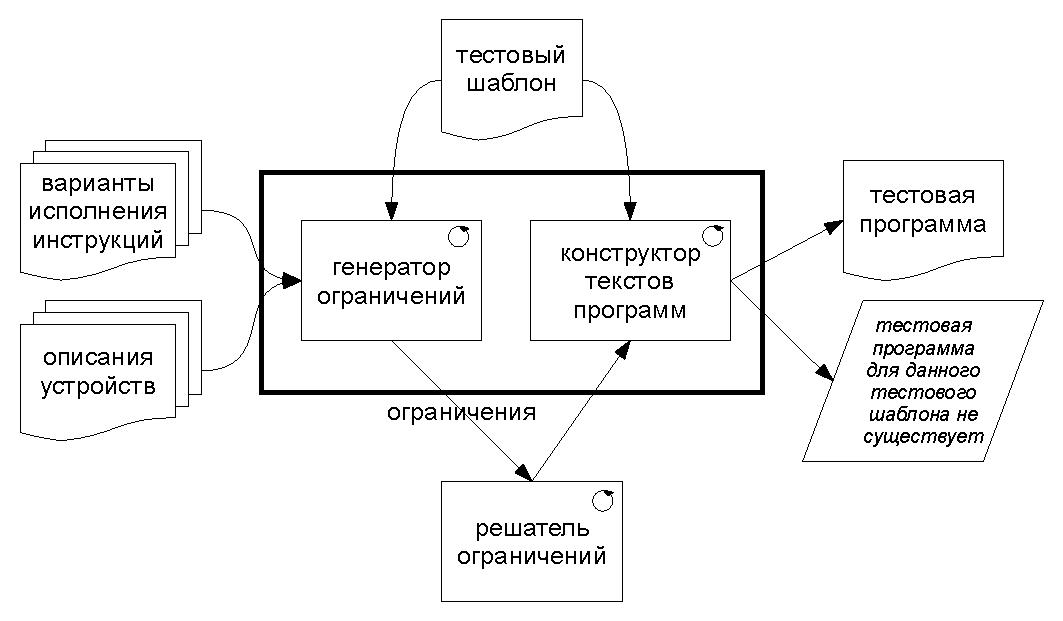
\includegraphics[width=0.8\textwidth]{2.theor/scheme}
  \caption{Программное средство для генерации тестовых программ}\label{fig:gen_scheme}
\end{figure}

Согласно схеме на рисунке~\ref{fig:gen_scheme} построение тестовой программы осуществляется следующим образом:
\begin{enumerate}
  \item \cmpn{Генератор ограничений} принимает на вход тестовый шаблон, описания вариантов исполнения инструкций и описания устройств подсистемы управления памяти и строит ограничения;
  \item Ограничения передаются на вход \cmpn{Решателю ограничений}; он определяет совместность данных ему ограничений; если ограничения несовместны, результатом его работы является сообщение о несовместности ограничений; если ограничения совместны, то он строит одно решение ограничений и сообщает это решение в качестве результата своей работы;
  \item \cmpn{Конструктор текстов программ} получает на вход тестовый шаблон и результат работы \cmpn{Решателя ограничений}; если \cmpn{Решатель ограничений} сообщил о несовместности ограничений, то \cmpn{Конструктор текстов программ} сообщает о несуществовании тестовой программы для данного тестового шаблона; иначе \cmpn{Конструктор текстов программ} на основе тестового шаблона по переданному \cmpn{Конструктору} решению ограничений строит тестовую программу, соответствующую тестовому шаблону.
\end{enumerate}

\begin{figure}[h] \center
  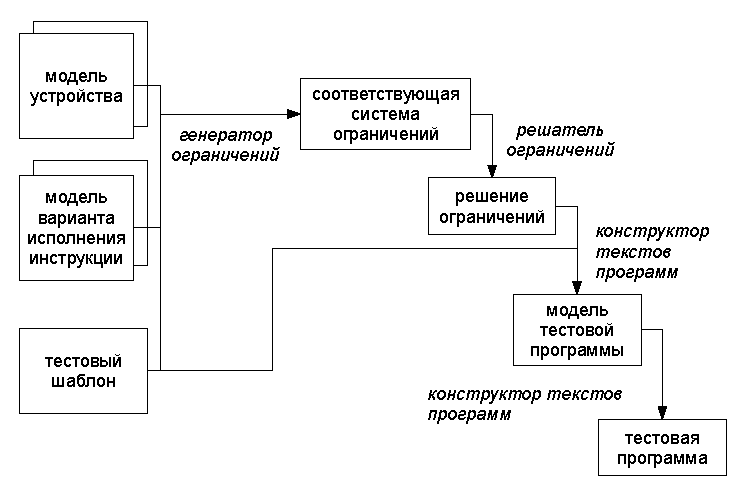
\includegraphics[width=0.8\textwidth]{2.theor/scheme2}
  \caption{Модели и задачи компонентов программного средства для генерации тестовых программ}\label{fig:models_tasks}
\end{figure}

Поставленная в разделе~\ref{sec:problem_refinement} задача решалась за счёт выбора специальных моделей (для вариантов исполнения инструкций, содержимого устройств подсистемы управления памяти и тестовой программы) и алгоритмов на основе этих моделей. На рисунке~\ref{fig:models_tasks} представлено место моделей в процессе генерации тестовой программы и задачи, которые решают компоненты описываемой здесь программной системы для генерации тестовых программ. В разделе~\ref{sec:state_model_section} будут даны формальные определения \emph{модели вариантов исполнения инструкций} и \emph{модели устройств}. В разделе~\ref{sec:constraints_generation_section} будет дано формальное определение \emph{системы ограничений, соответствующей} тестовому шаблону, моделям вариантов исполнения инструкций и моделям устройств. Неформально говоря, это такая система ограничений, которая эквивалентным образом выражает все ограничения на начальное состояние микропроцессора, содержащиеся в тестовом шаблоне и моделях. Задачей компонента \cmpn{Генератор ограничений} является построение системы ограничений, соответствующей тестовому шаблону, моделям вариантов исполнения инструкций и моделям устройств. Задачей \cmpn{Решателя ограничений} является разрешение этой системы ограничений. В разделе~\ref{?????} будет дано формальное определение \emph{модели тестовой программы} и \emph{модели тестовой программы, соответствующей решению ограничений и тестовому шаблону}. Неформально говоря, модель тестовой программы состоит из тестового шаблона, у каждой инструкции которого указаны значения ее аргументов, и последовательности адресов, по которым надо обратиться перед инструкциями тестового шаблона, и начальные значения регистров. Модель тестовой программы соответствует тестовому шаблону и решению ограничений, если в модели тестовой программы присутствует та же последовательность инструкций, а значения аргументов инструкций, адреса и начальные значения регистров взяты из решения ограничений. В разделе~\ref{????} будет дано формальное определение тестовой программы, соответствующей модели тестовой программы. Неформально говоря, это такая тестовая программа, которая исполняется в точном соответствии с моделью тестовой программы. Задачами компонента \cmpn{Конструктор тестовой программы} являются:
\begin{enumerate}
  \item построение модели тестовой программы, соответствующей тестовому шаблону и решению ограничений;
  \item построение тестовой программы, соответствующей модели тестовой программы.
\end{enumerate}




\section{Моделирование устройств подсистемы \\управления памяти и вариантов исполнения инструкций}\label{sec:state_model_section}

В данном разделе будут даны формальные определения ряда моделей%, будет уточнено определение тестового шаблона с учетом того, что эти шаблоны используются для тестирования подсистем управления памяти
. Будет дан ряд примеров и очерчена область применимости моделей.

\subsubsection*{Модель устройства подсистемы управления памяти}

%% определяется структура и содержание модельного состояния устройства

Назовем \emph{структурой поля} пару $(N, B)$, где $N$ --- произвольное имя, $B \in \mathds{N}$. $N$ будем называть \emph{именем} поля, $B$ --- \emph{битовой длиной} поля.

Назовем \emph{структурой строки} пару $(K, D)$, где $K$ и $D$ --- множества полей такие, что все поля в $K \cup D$ имеют разные имена. $K$ будем называть \emph{полями ключа}, $D$ будем называть \emph{полями данных}.

Назовем \emph{структурой региона} пару $(w, S)$, где $w \in \mathds{N}$, $S$ --- структура строки. $w$ будем называть \emph{ассоциативностью}.

Назовем \emph{структурной частью модели устройства} (или, \emph{структурой таблицы}) пару $(R, r)$, где $R \in \mathds{N} \cup \{0\}$, $r$ --- структура региона. Будем называть число $2^R$ \emph{количеством регионов}.

Назовем \emph{состоянием поля} со структурой $(N, B)$ целое число $v$ такое, что $v \geqslant 0$ и $v < 2^B$.

Назовем \emph{состоянием строки} со структурой $(K, D)$ пару $(k, d)$, где $K = \{K_1, K_2, ..., K_n\}$, $D = \{D_1, D_2, ..., D_m\}$, $k = \{k_1, k_2, ..., k_n\}$, $d = \{d_1, d_2, ..., d_m\}$, $k_i$ является состоянием поля $K_i$ для всех $i = 1, 2, ..., n$, $d_j$ является состоянием поля $D_j$ для всех $j = 1, 2, ..., m$.

Назовем \emph{состоянием региона} со структурой $(w, S)$ последовательность $\langle s_1,$ $s_2, ..., s_w\rangle$, где $r_i$ --- состояние строки со структурой $S$, $i = 1, 2, ..., w$, все состояния строк $s_j$ для $j = 1, 2, ..., w$ различные.

Назовем \emph{предикатом соответствия строки ключу} предикат $KM(k, \kappa)$, где $(k,d)$ --- состояние строки, $\kappa = (\kappa_1, \kappa_2, ..., \kappa_p)$, $\kappa_i \in \mathds{N} \cup \{0\}$, $i = 1, 2, ..., p$. Будем называть $\kappa$ \emph{ключом обращения}.

Назовем \emph{модельным состоянием устройства} со структурной частью $ST = (R, r)$ и предикатом соответствия строки ключу $KM$ последовательность $L = \langle r_0, r_1, ..., r_{2^R-1} \rangle$, где $r_i$ --- состояние региона со структурой $r$, $i = 0, 1, ..., 2^R{-}1$, и для любого состояния региона $r_i = \langle s_1, s_2, ..., s_w \rangle$ и для любого ключа обращения $\kappa$ не существует разных $s'$ и $s''$ из последовательности $r_i$ c состояниями полей ключей $k'$ и $k''$ соответственно таких, что $KM(k', \kappa)$ и $KM(k'', \kappa)$ истинны.


%% далее определяем правильные цепочки состояний
%%    с помощью определения правильных переходов между состояниями
%% > в результате будет определена `стратегия вытеснения'

Далее определим понятие <<стратегии вытеснения>> и ряда функций над модельными состояниями устройств.

Функция $hit: S \times \kappa \rightarrow S$, где $S$ --- состояние региона, $\kappa$ --- ключ обращения, определенная на тех парах $(S, \kappa)$, что в $S$ есть состояние строки $s = (k,d)$ такое, что $KM(k, \kappa)$ истинно, причем множество состояний строк в $hit(S, \kappa)$ и в $S$ одинаковые. Будем говорить, что в функции $hit$ осуществляется \emph{обращение к строке} $s$.

Функция $load: S \times \kappa \times dL \rightarrow S$, где $S$ --- состояние региона, $\kappa$ --- ключ обращения, $dL$ --- состояние полей данных, определенная на тех тройках $(S, \kappa, dL)$, что в $S$ есть состояние строки $s = (k,d)$ такое, что $KM(k, \kappa)$ истинно и $d = dL$, причем $load(S, \kappa, dL) = hit(S, \kappa)$. Будем говорить, что в функции $load$ осуществляется \emph{обращение к строке} $s$.

Функция $store: S \times \kappa \times dS \rightarrow S$, где $S$ --- состояние региона, $\kappa$ --- ключ обращения, $dS$ --- состояние полей данных, определенная на тех тройках $(S, \kappa, dS)$, что в $S$ есть состояние строки $s = (k,d)$ такое, что $KM(k, \kappa)$ истинно, причем выполнено следующее свойство: обозначим $store(S, \kappa, dS) = \langle r'_0, r'_1, ..., r'_{2^R-1}\rangle$ и $hit(S, \kappa) = \langle r''_0, r''_1, ..., r''_{2^R-1}\rangle$, $r''_i = s$, тогда $r'_j = r''_j$ для $j = 0, 1, ..., 2^R{-}1$, $j \neq i$, $r'_i = (k, dS)$. Будем говорить, что в функции $store$ осуществляется \emph{обращение к строке} $s$.

Функция $miss: S \times \kappa \rightarrow S$, где $S$ --- состояние региона, $\kappa$ --- ключ обращения, определенная на тех парах $(S, \kappa)$, что в $S$ нет состояния строки $s = (k,d)$ такого, что $KM(k, \kappa)$ истинно, и $miss(S, \kappa) = S$.

Назовем \emph{правилом определения вытесняемой строки} функцию $EV : S \rightarrow s$, где $S$ --- состояние региона, $s$ является состоянием одной из строк в $S$.

Функция $replace: S \times \kappa \times dR \rightarrow S$, где $S$ --- состояние региона, $\kappa$ --- ключ обращения, $dR$ --- состояние полей данных, определенная на тех тройках $(S, \kappa, dR)$, что в $S$ нет состояния строки $s = (k,d)$ такого, что $KM(k, \kappa)$ истинно, в состоянии региона $replace(S, \kappa, dR)$ есть состояние строки $s' = (\kappa, dR)$ и множество состояний строк в $S$ без состояния строки $EV(S)$ равно множеству состояний строк в $replace(S, \kappa, dR)$ без $s'$.

Назовем \emph{стратегией вытеснения} тройку функций $(hit, replace, EV)$.

Далее определим ряд семейств бинарных отношений над модельными состояниями устройств (другими словами, определим ряд \emph{параметризованных} бинарных отношений над модельными состояниями устройств, это означает, что каждому отношению будет сопоставлен ряд чисел и векторов чисел). Все определяемые далее бинарные отношения должны быть функциями, т.е. они должны определять однозначное соответствие (но не обязательно взаимно однозначное соответствие). По этой причине эти отношения будут далее в том числе использоваться как \emph{операции} над модельным состоянием.

Назовем \emph{отношением успешного обращения без данных} $Hit_{\kappa, \rho}$ множество пар модельных состояний $(L', L'')$, где $\kappa$ --- ключ обращения, $\rho$ --- целое число, $L' = \langle r'_0, r'_1, ..., r'_{2^R-1} \rangle$, $L'' = \langle r''_0, r''_1, ..., r''_{2^R-1} \rangle$, в которых выполнены все 3 следующие свойства:
  \begin{enumerate}
    \item $r''_i = r'_i$ для $i = 0, 1, 2, ..., 2^R{-}1$, $i \neq \rho$;
    \item в состоянии региона $r'_{\rho}$ существует строка $s = (k,d)$, для которой истинно $KM(k, \kappa)$;
    \item $r''_{\rho} = hit(r'_{\rho}, \kappa)$.
  \end{enumerate}

Назовем \emph{отношением успешного обращения с данными без изменения} (или, просто, \emph{отношением успешного обращения}) $HitLoad_{\kappa, \rho, dL}$ множество пар модельных состояний $(L', L'')$, где $\kappa$ --- ключ обращения, $\rho$ --- целое число, $dL$ --- состояние полей данных, $L' = \langle r'_0, r'_1, ..., r'_{2^R-1} \rangle$, $L'' = \langle r''_0, r''_1, ..., r''_{2^R-1} \rangle$, в которых выполнены все 3 следующие свойства:
  \begin{enumerate}
    \item $r''_i = r'_i$ для $i = 0, 1, 2, ..., 2^R{-}1$, $i \neq \rho$;
    \item в состоянии региона $r'_{\rho}$ существует строка $s = (k,d)$, для которой истинно $KM(k, \kappa)$ и $d = dL$;
    \item $r''_{\rho} = load(r'_{\rho}, \kappa, dL)$.
  \end{enumerate}

Назовем \emph{отношением успешного обращения без данных с изменением}\\ $HitStore_{\kappa, \rho, dS}$ множество пар модельных состояний $(L', L'')$, где $\kappa$ --- ключ обращения, $\rho$ --- целое число, $dS$ --- состояние полей данных, $L' = \langle r'_0, r'_1, ..., r'_{2^R-1} \rangle$, $L'' = \langle r''_0, r''_1, ..., r''_{2^R-1} \rangle$, в которых выполнены все 3 следующие свойства:
  \begin{enumerate}
    \item $r''_i = r'_i$ для $i = 0, 1, 2, ..., 2^R{-}1$, $i \neq \rho$;
    \item в состоянии региона $r'_{\rho}$ существует строка $s = (k,d)$, для которой истинно $KM(k, \kappa)$;
    \item $r''_{\rho} = store(r'_{\rho}, \kappa, dS)$.
  \end{enumerate}

Назовем \emph{отношением успешного обращения с данными с изменением} (или, просто, \emph{успешного обращения с изменением}) $HitLoadStore_{\kappa, \rho, dL, dS}$ множество пар модельных состояний $(L', L'')$, где $\kappa$ --- ключ обращения, $\rho$ --- целое число, $dL$ и $dS$ --- два состояния полей данных устройства, $L' = \langle r'_0, r'_1, ..., r'_{2^R-1} \rangle$, $L'' = \langle r''_0, r''_1, ..., r''_{2^R-1} \rangle$, в которых выполнены все 3 следующие свойства:
  \begin{enumerate}
    \item $r''_i = r'_i$ для $i = 0, 1, 2, ..., 2^R{-}1$, $i \neq \rho$;
    \item в состоянии региона $r'_{\rho}$ существует строка $s = (k,d)$, для которой истинно $KM(k, \kappa)$ и $d = dL$;
    \item $r''_{\rho} = store(r'_{\rho}, \kappa, dS)$.
  \end{enumerate}

Назовем \emph{отношением неуспешного обращения без замещения} $Miss(\kappa, \rho)$ множество пар модельных состояний $(L', L'')$, где $\kappa$ --- ключ обращения, $\rho$ --- целое число, $L' = \langle r'_0, r'_1, ..., r'_{2^R-1} \rangle$, $L'' = \langle r''_0, r''_1, ..., r''_{2^R-1} \rangle$, в которых выполнены все 3 следующие свойства:
  \begin{enumerate}
    \item $r''_i = r'_i$ для $i = 0, 1, 2, ..., 2^R{-}1$, $i \neq \rho$;
    \item в состоянии региона $r'_{\rho}$ нет состояния строки $s = (k,d)$, для которой истинно $KM(k, \kappa)$;
    \item $r''_{\rho} = miss(r'_{\rho}, \kappa)$.
  \end{enumerate}

Назовем \emph{отношением неуспешного обращения с замещением}\\ $MissReplace(\kappa, \rho, dR)$ множество пар модельных состояний $(L', L'')$, где $\kappa$ --- ключ обращения, $\rho$ --- целое число, $dR$ --- состояние полей данных, $L' = \langle r'_0, r'_1, ...,$ $r'_{2^R-1} \rangle$, $L'' = \langle r''_0, r''_1, ..., r''_{2^R-1} \rangle$, в которых выполнены все 3 следующие свойства:
  \begin{enumerate}
    \item $r''_i = r'_i$ для $i = 0, 1, 2, ..., 2^R{-}1$, $i \neq \rho$;
    \item в состоянии региона $r'_{\rho}$ нет строки $s = (k,d)$, для которой истинно $KM(k, \kappa)$;
    \item $r''_{\rho} = replace(r'_{\rho}, \kappa, dR)$.
  \end{enumerate}


Назовем \emph{моделью устройства} (или, \emph{таблицей}) тройку $(ST, RP, KM)$, где $ST$ --- структурная часть модели устройства, $RP$ --- стратегия вытеснения, $KM$ --- предикат соответствия строки ключу.

%% теперь вводим конечный автомат, раз он фигурирует в результатах автореферата!

Из введенной модели устройства следует представление устройства подсистемы управления памяти \emph{в виде конечного автомата}. Множеством состояний такого конечного автомата является множество всех модельных состояний (так, как они определены выше) и состояние Fail. Одно из модельных состояний выбрано в качестве начального состояния. Неформально говоря, к устройству производятся <<обращения>> с целью загрузить данные из устройства по заданному ключу в заданном регионе или сохранить данные в устройстве по заданному ключу в заданному регионе. Каждому обращению будет соответствовать один переход в конечном автомате. Переход помечен символом load, если это обращение с целью загрузки данных, или символом store, если это обращение с целью сохранения данных. Кроме того, символы load и store снабжены параметрами. load снабжен двумя параметрами: $\kappa$ (ключом обращения) и $\rho$ (номером региона). store снабжен тремя параметрами: $\kappa$ (ключом обращения), $\rho$ (номером региона) и $\delta$ (состоянием полей данных). Выходной алфавит конечного автомата состоит из символов $HitLoad$, $HitStore$ и $MissReplace$. Символ $HitLoad$ снабжен параметром $\delta$ (состояние полей данных). Функция переходов конечного автомата определено соответственно определениям отношений $HitLoad$, $HitStore$ и $MissReplace$, а именно:
  \begin{itemize}
    \item если для модельного состояния $L'$ существует такое модельное состояние $L''$, что $(L', L'') \in Hit_{\kappa, \rho}$, то из состояния $L'$ по входу load$(\kappa, \rho)$ осуществляется переход в состояние $L''$, при этом выходом является $HitLoad(\delta)$, где $\delta$ --- состояние полей данных такое, что $(L', L'') \in HitLoad_{\kappa, \rho, \delta}$; такой переход будет называться далее \emph{успешным обращением без изменения} (или, просто, \emph{успешного обращения});
    \item если для модельного состояния $L'$ не существует модельное состояние $L''$ такое, что $(L', L'') \in Hit_{\kappa, \rho}$, то из состояния $L'$ по входу load$(\kappa, \rho)$ осуществляется переход в состояние Fail;
    \item если для модельного состояния $L'$ существует такое модельное состояние $L''$, что $(L', L'') \in HitStore_{\kappa, \rho, \delta}$, то из состояния $L'$ по входу store$(\kappa, \rho, \delta)$ осуществляется переход в состояние $L''$, при этом выходом является\\ $HitStore$; такой переход будет называться далее \emph{успешным обращением c изменением};
    \item если для модельного состояния $L'$ существует такое модельное состояние $L''$, что $(L', L'') \in MissReplace_{\kappa, \rho, \delta}$, то из состояния $L'$ по входу store$(\kappa, \rho, \delta)$ осуществляется переход в состояние $L''$, при этом выходом является $MissReplace$; такой переход будет называться далее \emph{неуспешным обращением};
    \item все переходы из Fail ведут в Fail.
  \end{itemize}

Из определения отношений $HitStore$ и $MissReplace$ следует, что для любых $\kappa$, $\rho$, $\delta$ и для любого состояния $L'$, отличного от Fail, всегда есть либо переход из $L'$, помеченный $HitStore(\kappa, \rho, \delta)$, либо переход из $L'$, помеченный $MissReplace(\kappa, \rho, \delta)$.

Введенный таким образом конечный автомат позволяет по цепочке обращений в устройство из некоторого состояния определить, является ли эта цепочка обращений допустимой (т.е. приводит ли она в состояние Fail) и какие из обращений в этой цепочке были успешными, а какие были неуспешными.

% примеры моделей для устройств давать не буду, т.к. слишком много надо пояснять (почему LRU моделируется таким способом, почему регионы с вытеснением - это строки секций по одному и тому же индексу и т.д.)
% но можно ли тут сказать, что эту модель можно построить для практически полезных устройств? (кэш-память, TLB в MIPS, оперативная память)

% нотация
Для программной системы построения тестовых программ по тестовым шаблонам устройство подсистемы управления памяти должно быть представлено в рамках определенной в этом разделе модели устройства. Модель должна быть записана в виде \emph{описания устройства}. Описание устройства состоит из предиката соответствия строки ключу keyMatch и из пар <<название параметра = значение параметра>> для следующих параметров:
\begin{itemize}
    \item policy --- идентификатор, представляющий стратегию вытеснения (\LRU, \FIFO, \PseudoLRU); в число этих идентификаторов добавлен идентификатор none, он означает такую <<стратегию вытеснения>>, в которой нет функции replace и, соответственно, нет отношения $MissReplace$ (этот частный случай удобен при моделировании оперативной памяти, где отношения $Miss$ и $MissReplace$ по определению невозможны и при моделировании устройств, в которых неуспешные обращения не приводят к замещению);
    \item regionbits --- первый компонент структурной части модели устройства (двоичный логарифм количества регионов);
    \item lines --- количество строк в регионе (первый компонент структуры региона);
    \item line --- структура строки (для каждого поля указывается название, битовая длина, поле ли это ключа или поле данных).
%    \item keyMatch --- предикат от аргументов операции обращения и полей ключа строки; он истинен в том и только том случае, когда строка соответствует аргументам операции (тегам физического адреса, номерам виртуальных страниц и т.п.).
\end{itemize}

Пример описания кэш-памяти:
\begin{verbatim}
table L1 {
  policy = LRU;
  regionbits = 7;
  lines = 4;
  line( tag:24:key, d:32:data );
  keyMatch(kappa_tag:24) { kappa_tag = tag };
}
\end{verbatim}

Строка кэш-памяти состоит из поля tag, оно является полем ключа, и поля d. Ключ обращения состоит из одного компонента (kappa\_tag), его битовая длина равна 24 (т.е. kappa\_tag принимает целые значения от 0 до $2^{24}{-}1$. Ключ обращения соответствует строке, если kappa\_tag равен полю tag. Стратегия вытеснения LRU определяет такие правила перестановки строк, что в функции $replace$ замещается строка, последнее обращение к которой произошло раньше последнего обращения к любой другой строке региона. Детальное рассмотрение этой и других стратегий вытеснения будет сделано в разделе~\ref{sec:policy_table}.

%%% нужны пояснения ???

%Рассуждая для кэш-памяти (ее структура описана в разделе~\ref{section:cache}), строками будут кэш-строки с тегами адресов. Регион будут составлять кэш-строки из всех секций, расположенные по одному и тому же индексу. Количество строк в регионе  равно количеству секций, т.е. ассоциативности кэш-памяти $w$. Количество регионов равно количеству кэш-строк в секции.
%
%Буфер трансляции (TLB) в микропроцессорах архитектуры MIPS64~\cite{mips64III} состоит из строк, каждая строка содержит ряд полей, в том числе половину номера виртуальной страницы $v$, номер физического кадра, соответствующего виртуальной странице с номером $2v$, и номер физического кадра, соответствующего виртуальной странице с номером $2v+1$. Обращение в буфер происходит по некоторому виртуальному адресу. Если его половина присутствует в одной из строк TLB, то вычисляется физический адрес на основе одного из номеров физических кадров той же строки. Эту ситуацию будем считать <<попаданием>>. Если его половине не присутствует ни в одной из строк TLB, ситуацию будем считать <<промахом>>. При этом одна из строк будет вытеснена и заменена другой (это делается программно так же, как показано на рисунке~\ref{fig:blocks_init_examples}. Поэтому буфер трансляции адресов в микропроцессорах архитектуры
%MIPS64 моделируется таблицей из одного региона, каждая его строка состоит из полей \texttt{r}, \texttt{vpn/2}, \texttt{g}, \texttt{asid}, \texttt{pfn}$_0$, \texttt{CCA}$_0$, \texttt{v}$_0$, \texttt{pfn}$_1$, \texttt{CCA}$_1$, \texttt{valid}$_1$ и других.
%
%Упор на вытеснение сделан неслучайно: как показано в разделе~\ref{section:cache}, ряд важных ошибок связан именно с некорректной реализацией вытеснения. Предлагаемые здесь модели составляются для устройств подсистемы управления памяти, обладающих вытеснением. Это кэш-память всех уровней, таблицы трансляции адресов. Таким же образом можно смоделировать и оперативную память: строка такой таблицы содержит физический адрес и данные по нему, каждый регион состоит из одной строки.

%Описание модели уже упомянутого буфера трансляции адресов микропроцессоров архитектуры
%MIPS64 выглядит следующим образом:
%\begin{verbatim}
%table TLB
%{
%    line(   r:2:key, vpnd2:28:key, g:1:key, asid:4:key,
%            pfn0:24:data, cca0:3:data, valid0:1:data,
%            pfn1:24:data, cca1:3:data, valid1:1:data );
%    regionbits = 0;
%    policy = none;
%    lines = 48;
%    keyMatch(r:2, vpnd2:28) { .... };
%}
%\end{verbatim}
%
%Предикат keyMatch будет приведен чуть позже, когда будет описан для этого язык.




\subsubsection*{Модель варианта исполнения инструкций}

Напомню, что вариант исполнения инструкции --- это ограничение на значения аргументов инструкции и состояния микропроцессора, перед инструкцией и после нее.

%Здесь будет дано определение модели варианта исполнения инструкции.

%Представление варианта исполнения инструкции в рамках этой модели позволит увеличить при автоматизации построения тестовой программы для тестового шаблона

Назовем \emph{моделью варианта исполнения инструкции} для моделей устройств $M_1, M_2, ..., M_n$ пятерку $(Y, X, U, P, S)$, где
  \begin{itemize}
    \item $Y$ --- конечное множество переменных (множество \emph{выходных переменных});
    \item $X$ --- конечное множество переменных (множество \emph{входных переменных}), $X \cap Y = \varnothing$;
    \item $U$ --- конечное множество переменных (множество \emph{промежуточных переменных}), $U \cap Y = \varnothing$, $U \cap X = \varnothing$;
    \item $P$ --- ограничение над переменными $X \cup Y \cup U$;
    \item $S$ --- это множество троек $(M, r, p)$, где $M \in \{M_1, M_2, ..., M_n\}$, $r \in \{Hit,$ $HitLoad, HitStore, HitLoadStore, Miss, MissReplace\}$, $p$ --- это либо пара $(\kappa, \rho)$ при $r \in \{Hit, Miss\}$, либо тройка $(\kappa, \rho, d)$ при $r \in \{HitLoad,$ $HitStore, MissReplace\}$, либо четверка $(\kappa, \rho, dL, dS)$ при $r = HitLoadStore$, $\kappa$, $d$, $dL$, $dS$ --- последовательности переменных из множества $X \cup Y \cup U$, $\rho \in X \cup Y \cup U$, причем нет двух троек с одинаковым компонентом $M$.
  \end{itemize}

Тем самым модель указывает, что в рамках варианта исполнения инструкции допустим лишь определенный вид изменения модельного состояния устройств ($Hit$, $HitLoad$, $HitStore$, $HitLoadStore$, $Miss$ и $MissReplace$).

% нотация и семантика
Как и модели устройств, модели вариантов исполнения инструкций должны быть описаны на специальном языке для их использования в программной системе построения тестовых программ. Грамматика языка описания вариантов исполнения инструкции в виде расширенной формы Бэкуса-Наура приведена в приложении~\ref{sec:syntax}. Описание варианта исполнения инструкции состоит из двух частей: заголовка и тела описания. Заголовок состоит из объявлений аргументов инструкции. Объявление аргумента состоит из имени внутри данного описания и битовой длины аргумента. Аргументы в описаниях вариантов исполнения инструкций аналогичны формальным параметрам процедур в языке Паскаль с передачей аргументов по ссылке. Тело описания варианта исполнения инструкции состоит из последовательности \emph{операторов} над переменными-битовыми строками (let, assume) и операторов-обращений (hit, miss). Операторы над переменными-битовыми строками задают ограничение $P$, а операторы-обращения задают последовательность $\langle (r_i, p_i) \rangle_{i=1}^n$ (обозначения из определения модели варианта исполнения инструкции).

Семантика описаний вариантов исполнения инструкций представлена на языке RSL~\cite{RSL} в приложении~\ref{sec:semantics}. Назовем \emph{допустимым модельным состоянием} для модели варианта исполнения инструкции $(Y, X, U, P, S)$ вектор из значений всех переменных множества $X \cup Y \cup U$ и для каждой модели устройств подсистемы управления памяти бесконечная последовательность модельных состояний с указанием на одно из модельных состояний как на <<текущее>>. Каждому оператору в описании варианта исполнения инструкции сопоставим пару множеств допустимых модельных состояний $(PreS, PostS)$, причем $PostS \subseteq PreS$. Множество $PostS$ для произвольного (не последнего) оператора в описании варианта исполнения инструкции равно множеству $PreS$ для следующего оператора в этом же описании варианта исполнения инструкции. В приложении~\ref{sec:semantics} на языке RSL дано формальное определение допустимого модельного состояния и отношений над парами множеств допустимых модельных состояний $(PreS, PostS)$ для каждого оператора. Далее будут рассмотрены эти отношения для каждого оператора.

По определению множество допустимых модельных состояний $PostS$ последнего оператора в описании варианта исполнения инструкции включает лишь те модельные состояния устройств подсистемы управления памяти и значения переменных, из которых выполнены все операторы описания варианта исполнения инструкции. Если $PreS$ первого оператора в описании варианта исполнения инструкции включает все возможные допустимые модельные состояния, то $PostS$ последнего оператора этого описания варианта исполнения инструкции включает те и только те модельные состояния, на которых выполнены все операторы варианта исполнения инструкции. Описанию варианта исполнения инструкции соответствуют 2 множества допустимых модельных состояний: $PreS$ первого оператора в этом варианте исполнения инструкции и $PostS$ последнего оператора того же варианта исполнения инструкции. В тестовом шаблоне описания вариантов исполнения инструкций расположены в заданной последовательности, в которой $PostS$ для произвольного (не последнего) варианта исполнения инструкции совпадает с $PreS$ следующего за ним варианта исполнения инструкции. Тем самым, если $PreS$ первого описания варианта исполнения инструкции включает все возможные допустимые модельные состояния, то $PostS$ последнего описания варианта исполнения инструкции включает те и только те допустимые модельные состояния, на которых выполнены все варианты исполнения инструкции --- каждое такое допустимое модельное состояние задает \emph{начальное} состояний микропроцессора, из которого инструкции тестового шаблона будут исполняться согласно указанным вариантам исполнения. В это начальное состояние микропроцессора входят значения переменных, соответствующих регистрам микропроцессора, и первые элементы в последовательностях модельных состояний устройств.

$PostS$ \emph{оператора допущения} (\texttt{assume : boolexpr;}) равно множеству тех состояний из $PreS$, в которых для значений переменных выполнено логическое выражение \texttt{boolexpr}.

Входные и выходные переменные должны быть объявлены в заголовке описания варианта исполнения инструкции. А промежуточные переменные появляются внутри описаний вариантов исполнения инструкции --- для этого служит \emph{оператор объявления нового имени} let. Этот оператор имеет две формы: явную (\texttt{var <- expr;}) и неявную (\texttt{let var : BITLEN;}), \texttt{var} --- это имя переменной, \texttt{expr} --- выражение, \texttt{BITLEN} --- натуральное число. Оператор let в неявной форме объявляет промежуточную переменную \texttt{var} (т.е. в операторах описания варианта исполнения инструкции, расположенных до этого оператора let, переменной \texttt{var} нельзя пользоваться, после этого оператора --- можно) и фиксирует битовую длину ее значений, т.е. переменная может принимать любое целое значение от 0 до $2^{\mbox{\texttt{BITLEN}}}-1$. Иными словами, для оператора let в неявной форме $PostS$ равно $PreS$, причем все модельные состояния из $PostS$ отличаются лишь значением переменной \texttt{var} и среди всех модельных состояний из $PostS$ переменная \texttt{var} принимает все целые значения от 0 до $2^{\mbox{\texttt{BITLEN}}}-1$. Оператор let в явной форме является краткой записью такой последовательности операторов: \texttt{let var: BITLEN; assume: var = expr;}.

Операторам-обращения соответствуют следующие отношения над парами множеств модельных состояний $(PreS, PostS)$:
\begin{itemize}
  \item $PostS$ \emph{оператора попадания} \texttt{hit<table>(key, region) \{[loaded(} \\ \texttt{datafields)] [storing(datafields)]\}} равно множеству тех состояний из $PreS$, в которых текущее модельное состояния устройства table и следующее за ним модельное состояние устройства table находятся в отношении $p \in \{Hit, HitLoad, HitStore, HitLoadStore\}$, в этих отношениях состояние полей ключа $\kappa$ равно значению выражения \texttt{key} от значений переменных в допустимом модельном состоянии, а значение номера региона $\rho$ равно значению выражения \texttt{region} от значений переменных в допустимом модельном состоянии; синтаксис оператора попадания допускает наличие и отсутствие \texttt{loaded(datafields)} и \texttt{storing(datafields)}; если эти обе части отсутствуют, то $p = Hit$, если присутствует только \texttt{loaded}, то $p = HitLoad$, если присутствует только \texttt{storing}, то $p = HitStore$, в противном случае $p = HitLoadStore$, $datafields$ --- это последовательность выражений, задающая состояние полей данных;
  \item $PostS$ \emph{оператора промаха} \texttt{miss<table>(key, region) \{[replacing(} \\ \texttt{datafields)]\}} равно множеству тех состояний из $PreS$, в которых текущее модельное состояния устройства table и следующее за ним модельное состояние устройства table находятся в отношении $p \in \{Miss,$ $MissReplace\}$, в этих отношениях состояние полей ключа $\kappa$ равно значению выражения \texttt{key} от значений переменных в допустимом модельном состоянии, а значение номера региона $\rho$ равно значению выражения \texttt{region} от значений переменных в допустимом модельном состоянии; синтаксис оператора попадания допускает наличие и отсутствие \texttt{replacing(}\\ \texttt{datafields)}; в случае отсутствия \texttt{replacing} $p = Miss$, в противном случае $p = MissReplace$, $datafields$ --- это последовательность выражений, задающая состояние полей данных.
\end{itemize}

Неформально говоря, вариант исполнения инструкции описывается как последовательность уточнений состояния (assume), объявлений новых переменных (let) и обращений к устройствам подсистемы управления памяти (hit, miss).

Для составления выражений boolexpr и expr определены следующие <<операции>>~\cite{my_syrcose_2008, my_isp_2008}:
\begin{itemize}
    \item битовые операции:
        \begin{itemize}
            \item выделение бита с заданным индексом: \texttt{x[i]} есть значение \texttt{i}'го бита битовой строки \texttt{x};
            \item выделение диапазона бит в заданных границах: \texttt{x[i..j]} есть битовая строка, составленная из последовательности бит строки \texttt{x} с номерами \texttt{i}, \texttt{i+1}, ..., \texttt{j};
            \item битовая конкатенация: \texttt{x || y} есть битовая строка, первые биты которой равны битам строки \texttt{x}, а последующие --- битам строки \texttt{y};
            \item битовая степень: \texttt{x\^{ }n} есть битовая строка, равная $\underbrace{\mbox{\texttt{x||x||...||x}}}_{\mbox{\texttt{n}}}$;
            \item знаковое расширение битового размера: \texttt{(n) x} есть строка, битовая длина которой равна \texttt{n} и в знаковом представлении значение этой строки совпадает со значением строки \texttt{x};
        \end{itemize}
    \item арифметические операции (суммирование, вычитание, умножение); суммирование и вычитание производится только над числами одинаковой битовой длины по модулю, равному степени двойки с показателем, равным этой битовой длине; умножение есть в беззнаковой  (\texttt{*+}) и знаковой (\texttt{*-}) форме и проводится также над числами одинаковой битовой длины, но точно;
    \item отношения сравнения (равенство/неравенство, сравнение на\\больше~-~меньше);
    \item логические связки конъюнкция и дизъюнкция.
\end{itemize}

В приложении~\ref{sec:xml} приведен пример описания варианта исполнения инструкции загрузки данных из памяти целиком.

% границы применимости
Область действия моделей вариантов исполнения инструкций и языка описания вариантов исполнения инструкций позволяет выразить ряд структурных и функциональных особенностей организации устройств подсистемы управления памяти  и функциональных особенностей инструкций обращения в память, а именно:
\begin{itemize}
    \item многоуровневая кэш-память: для каждого уровня кэш-памяти составляется своя модель устройства, в вариантах исполнения инструкций явно указывается, в какие уровни происходят обращения, а в какие нет;
    \item обращение в память с использованием виртуальной памяти и без ее использования: эти два случая различаются классом виртуальных адресов (трансляция одного класса виртуальных адресов выполняется при помощи TLB, а другого класса --- без TLB), для указания класса виртуальных адресов достаточно добавить в ограничение $P$ модели варианта исполнения инструкции условие на виртуальный адрес;
    \item сквозная запись в память (write-through) и отложенная запись в память (write-back): в структуре строки модели устройства для кэш-памяти и в структуре строки модели устройства для оперативной памяти надо указать поля данных, а в описаниях вариантов исполнения инструкций явно указать изменение состояний этих полей при помощи storing в операторе hit;
    \item дополнительные условия на состояния полей ключа и данных: эти условия добавляются с помощью оператора assume;
    \item virtually indexed virtually tagged - кэш-память --- это кэш-память, в которой ключ и регион обращения вычисляются по виртуальному, а не физическому адресу (соответствующие выражения для состояний полей ключа и номеров регионов указываются в операторах-обращениях).
\end{itemize}

Ряд особенностей организации устройств подсистемы управления памяти не удается выразить в модели устройств и моделях вариантов исполнения инструкций~\cite{my_ewdts_2009}. Среди них:
\begin{itemize}
%    \item псевдослучайных действий: псевдослучайное вытеснение, псевдослучайный выбор таблицы, к которой происходит обращение;
    \item временн\'{ы}е ограничения: например, в некоторых микропроцессорах\\ PowerPC~\cite{PowerPC} трансляция адреса выполняется в два этапа: эффективный адрес (он содержит номер сегментного регистра и смещение в сегменте) сначала преобразуется в линейный (в нем нет номера сегментного регистра), затем линейный --- в физический; причем имеется буфер, который хранит пары из эффективного и физического адресов; во время трансляции одновременно выполняется обращение в этот буфер и двухэтапная схема; физический адрес считывается из того устройства, где быстрее будет получен физический адрес; тестовая ситуация, предписывающая выполнение трансляции в устройстве быстрее/медленнее, нежели чем через другое устройство, невыразима с использованием предлагаемого формализма;
    \item циклические действия с переменным числом итераций в описании инструкций: такие действия часто встречаются при задании алгоритмов работы FPU, однако на основе анализа документации по разным архитектурам был сделан вывод, что инструкции обращения к памяти с потоком управления, включающим такие итеративные действия, не сводящиеся к поиску строк и их вытеснению, как это определяется в операторах попадания и промаха, практически не встречаются;
    \item кэш-память инструкций, совместная кэш-память (с данными и инструкциями): кэш-память инструкций предназначена для кэширования блоков инструкций, тегами в строках кэш-памяти инструкций являются битовые части адресов, по которым расположены в памяти эти инструкции; однако в тестовых шаблонах инструкции расположены друг за другом, что не позволяет выразить многие тестовые ситуации на кэш-память инструкций; иными словами, для целенаправленной генерации тестовых программ на кэш-память инструкций нужная иная постановка задачи --- иначе тестовые ситуации, иные тестовые шаблоны, что выходит за рамки данной работы.
\end{itemize}


% модель программы

% соответствие модели программы и шаблона




%Теперь переходим к языку описания формализованных вариантов исполнения инструкций (или просто, языку описания инструкций). На предыдущих этапах вариант исполнения задавался в виде последовательности неформализованных действий. Формализованное описание инструкции повторяет эту последовательность, внося ряд уточнений. В документации по микропроцессору вариант исполнения инструкции описывается на псевдокоде в виде последовательности преобразований-операторов, причем большая их часть --- это операторы над битовыми строками (например, значениями регистров, виртуальных адресов, физических адресов). Предлагаемое в диссертации описание следует этому же принципу: это последовательность операторов над битовыми строками и двух дополнительных операторов, специфичных блокам подсистемы управления памяти.


%Далее будет рассмотрен ряд примеров описаний некоторых вариантов инструкций обращения к памяти.
%
%Рассмотрим на примере, как строится описание варианта инструкции LW под названием l1hit. В документации написано, что формат инструкции LW следующий:
%\begin{verbatim}
%LW rt, offset(base)
%\end{verbatim}
%
%Эта инструкция загружает в регистр rt 32 бита из памяти по (виртуальному) адресу base{+}offset. Описание функциональности инструкции LW в документации приводится на специальном псевдокоде (см. рисунок~\ref{fig:lw_exmp}).
%
%\begin{figure}[h]
%\begin{tabular}{cl}
%    ${ }^1$ & \texttt{vAddr <- sign\_extend(offset) + GPR[base]}\\
%    ${ }^2$ & \texttt{if vAddr[1..0] != 0\^{ }2 then}\\
%    ${ }^3$ & \hspace{2cm} \texttt{SignalException(AddressError)}\\
%    ${ }^4$ & \texttt{endif}\\
%    ${ }^5$ & \texttt{(pAddr, CCA) <- AddressTranslation(vAddr, DATA, LOAD)}\\
%    ${ }^6$ & \texttt{pAddr <- pAddr[PSIZE-1..3] || (pAddr[2..0] xor}\\
%       & \hspace{5cm} \texttt{(ReverseEndian || 0\^{ }2) )}\\
%    ${ }^7$ & \texttt{memdoubleword <- LoadMemory(CCA, WORD, pAddr, vAddr, DATA)}\\
%    ${ }^8$ & \texttt{byte <- vAddr[2..0] xor (BigEndianCPU || 0\^{ }2)}\\
%    ${ }^9$ & \texttt{GPR[rt] <- sign\_extend(memdoubleword[31+8*byte..8*byte])}\\
%\end{tabular}
%\caption{Описание инструкции LW на псевдокоде из документации по MIPS64}\label{fig:lw_exmp}
%\end{figure}
%
%Это описание представляет собой последовательность операторов, которые изменяют значения переменных и внутреннее состояние микропроцессора. В этом описании присутствует оператор присваивания (он обозначен обратной стрелкой <-) и условный оператор if-then-endif, в then-ветви которого находится оператор исключительной ситуации SignalException, прерывающий исполнение этой инструкции. GPR[rt] и GPR[base] --- это выражения для получения значений регистров общего назначения с именами rt и base соответственно. Также используется ряд других операций и констант (они набраны прописными буквами).
%
%В отдельной главе документации (2.2 Operation Section Notation and\\Functions) содержится описание <<подпрограмм>> AddressTranslation и\\LoadMemory. В первой происходит трансляция виртуального адреса в физический, во второй происходит обращение в оперативную память по физическому адресу с использованием кэш-памяти. В другой главе документации (4. Virtual Memory) указано, что в этих подпрограммах задействуются следующие устройства подсистемы управления памяти:
%\begin{itemize}
%  \item кэш-память данных первого уровня (D-cache);
%  \item кэш-память инструкций первого уровня (I-cache);
%  \item кэш-память второго уровня, совместная для данных и инструкций (L2-cache);
%  \item общий буфер трансляции адресов (TLB);
%  \item буфер трансляции адресов данных (DTLB);
%  \item буфер трансляции адресов инструкций (ITLB).
%\end{itemize}
%
%Вариант l1hit будет означать такое исполнение инструкции LW, при котором трансляция адреса выполняется без обращения к TLB и DTLB, а при обращении в кэш-память первого уровня происходит кэш-попадание.
%
%Тем самым для тестового шаблона будет задействована кэш-память данных первого уровня, значит, надо смоделировать устройство D-cache. Устройства I-cache и L2-cache и все *TLB не задействованы в l1hit, поэтому их моделировать не нужно.
%
%Составляем модель D-cache. Для этого читаем документацию и выделяем из нее:
%\begin{itemize}
%  \item ассоциативность равна 4;
%  \item стратегия вытеснения --- LRU;
%  \item размер виртуального адреса --- 64 бита;
%  \item размер физического адреса --- 36 бит; из них биты с 35го по 12й дают тег, с 11го по 5й --- дают номер региона, с 4го по 0й дают смещение в кэш-строке.
%\end{itemize}
%
%Тем самым, модель кэш-памяти первого уровня будет следующей:
%\begin{verbatim}
%    table l1 {
%        line(tag:24:key);
%        regionbits = 7;
%        policy = LRU;
%        lines = 4;
%        keyMatch(key:24) { key = tag };
%    }
%\end{verbatim}
%
%Кроме того, нужно будет получить значения из памяти (в memdoubleword). Значит, нужно смоделировать оперативную память:
%\begin{verbatim}
%    table memory {
%        line(phys:33:key; memdw:64:data);
%        regionbits = 0;
%        policy = none;
%        lines = 8589934592;
%    }
%\end{verbatim}
%
%Для подготовки формального описания l1Hit надо в описании инструкции LW:
%\begin{enumerate}
%  \item выделить аргументы инструкции и их битовые длины;
%  \item определить значения <<констант>> (в данном случае это PSIZE,\\ ReverseEndian, BigEndianCPU, WORD);
%  \item выделить в потоке управления этого описания путь, соответствующий варианту исполнения l1hit;
%  \item формализовать <<подпрограммы>> AddressTranslation и LoadMemory в контексте l1hit;
%  \item выразить выделенный путь в потоке управления в виде последовательности операторов.
%\end{enumerate}
%
%Аргументов здесь три: offset, GPR[base] и GPR[rt]. Их битовые длины -- 16, 64 и
%64 (первое написано также на странице описания LW, а остальные аргументы суть
%GPR --- регистры общего назначения, чей битовый размер в MIPS64 равен 64).
%<<Константы>> PSIZE, ReverseEndian, BigEndianCPU являются частью режима работы
%микропроцессора в момент тестирования. Тем самым их значения надо искать в этом
%режиме. Путь в потоке управления должен быть таким, чтобы в него попал
%LoadMemory (чтобы произошло заявленное кэш-попадание в кэш-память первого
%уровня).
%
%Начинаем строить формализованное описание варианта l1hit. Объявления аргументов:
%\begin{verbatim}
%    base : 64;
%    offset : 16;
%    rt : 64;
%\end{verbatim}
%
%Начало описания пути \texttt{l1Hit} практически дословно повторяет документацию (строки 1--4 описания инструкции LW):
%\begin{verbatim}
%    vAddr <- (64)offset + base;
%    assume: vAddr[1..0] = 0^2;
%\end{verbatim}
%
%В строке 5 идет <<вызов подпрограммы>> \texttt{AddressTranslation}. В l1hit трансляция виртуального адреса в физический должна выполняться без
%обращения к TLB. Это означает, что надо специфицировать условия, при которых
%трансляция адреса выполняется именно таким образом, и результат этой трансляции.
%Условия и результат трансляции описаны в документации (глава 4. Virtual memory). А именно, такая
%трансляция выполняется тогда, когда биты виртуального адреса с 58го по 36й равны нулю. В качестве результата формируется значение новых переменных --- физического адреса \texttt{pAddr} и политики кэширования \texttt{cca}:
%\begin{verbatim}
%    assume: vAddr[58..36] = 0^23;
%    pAddr <- vAddr[35..0];
%    cca <- vAddr[63..61];
%\end{verbatim}
%
%От политики кэширования будет зависеть работа кэш-памяти и это действительно
%разные способы работы -- сквозная запись и отложенная запись, где-то
%производится запись в кэш-память и в оперативную память, где-то только в
%оперативную память. Но при \texttt{l1Hit} запись не производится и
%поэтому достаточно, чтобы кэш-память просто была задействована. Согласно
%документации это означает, что \texttt{cca} не должно равняться 2. Тем самым
%появляется еще одно условие про \texttt{AddressTranslation}:
%\begin{verbatim}
%    assume: cca != 2;
%\end{verbatim}
%
%В строке 6 идет изменение физического адреса с учетом \texttt{ReverseEndian}.
%<<Константа>> ReverseEndian соответствует режиму, в котором происходит
%тестирование. Т.е. в момент генерации теста значение \texttt{ReverseEndian}
%известно, его не нужно искать с помощью ограничений. Если тест будет исполняться
%в режиме с \texttt{ReverseEndian = 0}, то преобразование выполнять не надо, т.к.
%\texttt{pAddr <- pАddr[PSIZE-1..3]||(pAddr[2..0] xor (0||0\^{ }2))} эквивалентно
%\texttt{pAddr <- pАddr[PSIZE-1..0])}, а \texttt{PSIZE = 36} (из документации),
%т.е. \texttt{pАddr[PSIZE-1..0]} получается то же, что и \texttt{pАddr}.
%Рассмотрим более сложный случай ---\\ \texttt{ReverseEndian = 1} (кроме того, хотя в документации используется одно и то же имя для физического адреса до изменения и после, при формализации надо указать новое имя):
%\begin{verbatim}
%    pAddr2 <- pAddr[35..3] || (pAddr[2]+1) || pAddr[1..0];
%\end{verbatim}
%
%В строке 7 идет <<вызов подпрограммы>> \texttt{LoadMemory}. В \texttt{l1Hit} это должно быть лишь
%обращение в кэш-память первого уровня с попаданием и обращение в память за
%данными. Надо понять, что является ключами и регионами этих обращений. Читаем
%документацию по тому, как проводится обращение в кэш-память:
%\begin{verbatim}
%    tag <- pAddr2[35..12];
%    region <- pAddr2[11..5];
%    phys <- pAddr2[35..3];
%    let data:64;
%    hit<l1>(tag, region){};
%    hit<memory>(phys){loaded(memdw=data)};
%\end{verbatim}
%
%Неявная форма оператора let была использована для получения значения поля memdw. Приведенная последовательность операторов фиксирует, что при обращение в \texttt{l1} должно быть успешным и
%из памяти считывается 64 бита в переменную \texttt{memdw}.
%
%В строках 8 и 9 из этих 64 бит выбираются 32 бита  --- старшая половина или младшая --- на основе значения \texttt{vAddr[2..0]}:
%\begin{verbatim}
%    byte <- vAddr[2..0];
%    let word:32;
%    assume: byte = 0 and word = memdw[31..0]
%         or byte = 4 and word = memdw[63..32];
%    rt <- (64)word;
%\end{verbatim}
%
%Описание инструкции \texttt{LW} для \texttt{l1Hit} готово. В правой половине рисунка~\ref{fig:l1hit_model} изображено формализованное описание варианта l1hit. В левой половине  рисунка~\ref{fig:l1hit_model} для сравнения приведен путь выполнения инструкции KW, которому соответствует l1hit.
%
%\begin{figure}[h]
%\noindent\parbox{0.4\textwidth}{ \footnotesize \tt
%vAddr <- sign\_extend(offset) + GPR[base];\\
%assume: vAddr[1..0] = 0\^{}2;\\
%(pAddr, CCA) <- AddressTranslation( vAddr, DATA, LOAD );\\
%pAddr <- pAddr[PSIZE-1..3] || (pAddr[2..0] xor (ReverseEndian || 0\^{}2 ));\\
%memdoubleword <- LoadMemory(CCA, WORD, pAddr, vAddr, DATA);\\
%byte <- vAddr[2..0] xor (BigEndianCPU || 0\^{}2);\\
%GPR[rt] <- sign\_extend( memdoubleword[ 31+8*byte .. 8*byte ] );\\
%} \parbox{0.1\textwidth}{ \quad
%} \parbox{0.5\textwidth}{ \footnotesize \tt
%base : 64;\\
%offset : 16;\\
%rt : 64;\\
%\\
%vAddr <- (64)offset + base;\\
%assume: vAddr[1..0] = 0\^{}2;\\
%assume: vAddr[58..36] = 0\^{}23;\\
%pAddr <- vAddr[35..0];\\
%cca <- vAddr[63..61];\\
%assume: cca != 2;\\
%pAddr2 <- pAddr[35..3] ||\\
%\indent\hspace{1cm}(pAddr[2]+1) || pAddr[1..0];\\
%tag <- pAddr2[35..12];\\
%region <- pAddr2[11..5];\\
%phys <- pAddr2[35..3];\\
%let data:64;\\
%hit<l1>(tag, region)\{\};\\
%hit<memory>(phys)\{loaded(memdw=data)\};\\
%byte <- vAddr[2..0];\\
%let word:32;\\
%assume: byte = 0 and word = data[31..0]\\
%\indent\hspace{1cm}or byte = 4 and word = data[63..32];\\
%rt <- (64) word;}
%\caption{Описание варианта l1hit до и после полной формализации}\label{fig:l1hit_model}
%\end{figure}
%
%Другим примером будет предикат keyMatch для TLB микропроцессоров MIPS64:
%(\texttt{asid} является <<константой>> режима тестирования, для примера
%допустим, что она равна 10)
%
%\begin{verbatim}
%table TLB
%{
%    line(   r:2:key, vpnd2:28:key, g:1:key; asid:4:key,
%            pfn0:24:data, cca0:3:data, valid0:1:data,
%            pfn1:24:data, cca1:3:data, valid1:1:data );
%    regionbits = 0;
%    policy = none;
%    lines = 48;
%    keyMatch(r1:2, vpnd:28) { r1 = r and vpnd = vpnd2 and
%        (g = 1 or asid = 10)};
%}
%\end{verbatim}


\section{Метод построения ограничений}\label{sec:constraints_generation_section}

В этом разделе будет формально поставлена задача, которую решает компонент \cmpn{Генератор ограничений} (см. схему на рисунке~\ref{fig:gen_scheme}), описано ее решение (алгоритм построения ограничений), обоснована корректность этого решения и исследован ряд свойств этого решения.

Задачей компонента \cmpn{Генератор ограничений} является построение системы ограничений, решение которой позволило бы построить тестовую программу для тестового шаблона. Для этого система ограничений должна <<соответствовать>> тестовому шаблону. В разделе~\ref{?????} дается формальное определение системы ограничений, соответствующей тестовому шаблону и моделям вариантов исполнения инструкций и устройств.

Неформально говоря, целью составления и разрешения системы ограничений является поиск значений операндов инструкций (как входящих в тестовый шаблон, так и дополнительных, \emph{инициализирующих} микропроцессор, которые помещаются в тестовую программу перед инструкциями из тестового шаблона), при которых возникнет заданная тестовым шаблоном тестовая ситуация (т.е. инструкции тестового шаблона будут выполнены согласно указанным для них вариантам исполнения).  Существует набор инструментов~\cite{Z3, Yices}, которые позволяют решить ограничения, поэтому ограничения должны принадлежать классам ограничений, с которыми умеют работать эти инструменты (известно, что с ограничениями в битовой арифметике и с ограничениями в линейной арифметике эти инструменты умеют работать).

Поскольку количество инструкций в тестовом шаблоне конечно, то в этих инструкциях осуществляются обращения лишь к конечному числу регионов устройств подсистемы управления памяти. Тем самым, необязательно при помощи ограничений искать всё целиком модельное состояние каждого устройства. Вместо этого достаточно искать состояния лишь необходимых для опе-раторов-обращений регионов модельных состояний (поскольку по определению отношений над парами модельных состояний одно обращение к устройству <<работает>> лишь с одним регионом, а состояния остальных регионов не изменяется). В некоторых случаях нет необходимости даже искать и состояние региона целиком (например, если в тестовом шаблоне есть всего один оператор-обращение к региону, причем это оператор попадания, тогда достаточно в инициализирующих инструкциях обеспечить 1 инструкцию, которая обратится в этот регион и обеспечит попадание). В разделе~\ref{?????} дается алгоритм построения системы ограничений. В нем учитываются высказанные в данном абзаце идеи по уменьшению количества переменных в ограничениях и количество самих ограничений, что, тем самым, позволяеь сократить вычислительную сложность разрешения ограничений.

Исполнение инструкций конвейеризовано, поэтому расположенные рядом инструкции в действительности будут выполняться параллельно в конвейере. Однако в алгоритме генерации ограничений считается, что инструкции выполняются последовательно, а тестовые шаблоны составлены таким образом, чтобы при работе соответствующих шаблонам тестовых программ проявились все выраженные в шаблонах параллельные эффекты.

В разделе~\ref{?????} формулируется и доказывается теорема корректности алгоритма построения ограничений. Эта теорема обосновывает тот факт, что предлагаемый в разделе~\ref{?????} алгоритм строит систему ограничений, соответствующую тестовому шаблону и моделям вариантов исполнения инструкций и устройств.

В разделе~\ref{?????} формулируется теорема полноты алгоритма построения ограничений. Эта теорема обосновывает тот факт, что множество значений переменных в тестовом шаблоне, соответствующих решению системы ограничений (построенной согласно этому алгоритму), а, соответственно, и множество тестовых программ для этих значений переменных в тестовом шаблоне, исчерпывает все возможные тестовые программы, удовлетворяющие тестовому шаблону. Иными словами, если построенная алгоритмам система ограничений окажется несовместной, то для тестового шаблона и моделей вариантов исполнения инструкций и устройств на самом деле не существует ни одной удовлетворяющей им тестовой программы.

%Формализовав устройства подсистемы управления памяти и инструкции и составив тестовый шаблон, нужно определить те значения регистров и хранящиеся данные устройств, при которых исполнение инструкций, указанных в тестовом шаблоне, будет проходить согласно указанным там вариантам. Для этого составляется система ограничений, выражающая все необходимые условия на такие значения. В результате разрешения этой системы определяются искомые значения. В данном разделе описывается предлагаемый алгоритм построения ограничений для тестового шаблона. Исполнение инструкций конвейеризовано, поэтому расположенные рядом инструкции в действительности будут выполняться с существенной долей параллелизма. Однако в алгоритме генерации ограничений считается, что инструкции выполняются последовательно, а тестовые шаблоны составлены таким образом, чтобы при работе соответствующих им тестовых программ проявились все нужные параллельные эффекты.
%
%По каждому оператору алгоритм строит свою часть ограничений, которые выражают семантику этого оператора. Операторы обращений в устройства транслируются в ограничения без моделирования состояний устройств, несмотря на то, что определение этих операторов включало состояние устройства. Это позволяет существенно уменьшить количество переменных-битовых строк и размер ограничений и, тем самым, ускорить разрешение ограничений. Специальное представление выбрано и для начального содержимого устройств, а именно, последовательность обращений в это устройство. Поэтому в число переменных в ограничениях входят переменные, задающие аргументы этих, \emph{инициализирующих}, обращений: ключи, номера регионов. Для операторов \texttt{hit} и \texttt{miss} строятся ограничения на аргументы-ключи и номера регионов (эти ограничения должны гарантировать успешное обращение для \texttt{hit} и неуспешное --- для \texttt{miss}) и ограничения на аргументы-данные из секций loaded, storing и replacing (обращения по одинаковым адресам должны давать одинаковые данные, если они не были изменены). Ограничения на аргументы-ключи и аргументы-номера регионов строятся согласно следующим определениям операторов: \texttt{hit(k$_i$;R$_i$)} / \texttt{miss(k$_i$;R$_i$)} происходит, если
%\begin{itemize}
%\item[$(\alpha)$] перед ним есть обращение по тому же ключу (\texttt{k}$_i$) в тот же регион (\texttt{R}$_i$),
%\item[$(\beta)$] после которого и до этого обращения соответствующая строка \underline{не была} \underline{вытеснена} / \underline{была вытеснена} из таблицы.
%\end{itemize}
%
%Трансляция свойства $\alpha$ достаточно очевидна, трансляция свойства $\beta$ рассматривается в разделе~\ref{sec:usefulness_functions}.

\subsection{Алгоритмы}

При формулировке алгоритмов будут использоваться следующие обозначения:
\begin{itemize}
  \item <<||>> --- битовая конкатенация;
  \item $[\varphi] \equiv $ if $\varphi$ then 1 else 0 endif.
\end{itemize}

\subsubsection*{Система ограничений, соответствующая тестовому шаблону, моделям устройств и вариантов исполнения инструкций}

Пусть задан следующий тестовый шаблон из $q$ инструкций для моделей устройств $M_1,$ $M_2,$ ..., $M_p$:

$I^{(1)}~a_1^{(1)}~a_2^{(1)}~...~a_{ac_1}^{(1)}~\mbox{@}~c^{(1)}( y_1^{(1)}, ..., y_{yc_1}^{(1)}, x_1^{(1)}, ..., x_{xc_1}^{(1)}, u_1^{(1)}, ..., u_{uc_1}^{(1)})$

$I^{(2)}~a_1^{(2)}~a_2^{(2)}~...~a_{ac_2}^{(2)}~\mbox{@}~c^{(2)}( y_1^{(2)}, ..., y_{yc_2}^{(2)}, x_1^{(2)}, ..., x_{xc_2}^{(2)}, u_1^{(2)}, ..., u_{uc_2}^{(2)})$

. . . . .

$I^{(q)}~a_1^{(q)}~a_2^{(q)}~...~a_{ac_q}^{(q)}~\mbox{@}~c^{(q)}( y_1^{(q)}, ..., y_{yc_q}^{(q)}, x_1^{(q)}, ..., x_{xc_q}^{(q)}, u_1^{(q)}, ..., u_{uc_q}^{(q)})$

где для каждого $i = 1, 2, ..., q$ $Y^{(i)} = \{ y_1^{(i)}, ..., y_{yc_i}^{(i)} \}$, $X^{(i)} = \{ x_1^{(i)}, ..., x_{xc_i}^{(i)} \}$, $U^{(i)} = \{ u_1^{(i)}, ..., u_{uc_i}^{(i)} \}$, $ac_i = yc_i + xc_i$, $Y^{(i)} \cap X^{(i)} = \varnothing$, $Y^{(i)} \cap U^{(i)} = \varnothing$, $X^{(i)} \cap U^{(i)} = \varnothing$, $c^{(i)} = (Y^{(i)}, X^{(i)}, U^{(i)}, P^{(i)}, Q^{(i)})$,

и для любых $i, j = 1, 2, ..., q$ таких, что $i \neq j$, $Y^{(i)} \cap Y^{(j)} = \varnothing$, $X^{(i)} \cap X^{(j)} = \varnothing$, $U^{(i)} \cap U^{(j)} = \varnothing$, $Y = \bigcup_{i=1}^q Y^{(i)}$, $X = \bigcup_{i=1}^q X^{(i)}$, $U = \bigcup_{i=1}^q U^{(i)}$, $Y \cap X = \varnothing$, $Y \cap U = \varnothing$, $X \cap U = \varnothing$,

для каждого $i = 1, 2, ..., q$ аргументам инструкции $I^{(i)}$ сопоставлены аргументы $c^{(i)}$: аргументу $a_1^{(i)}$ сопоставлено $y_1^{(i)}$, аргументу $a_2^{(i)}$ сопоставлено $y_2^{(i)}$, и т.д.

Тогда систему ограничений, удовлетворяющую всем следующим свойствам, будем называть \emph{соответствующей} тестовому шаблону, моделям вариантов инструкций и моделям устройств:
  \begin{enumerate}
    \item множество переменных системы ограничений равно множеству $Y \cup X \cup U \cup t \cup r \cup d$, где $t = \bigcup_{i=1}^p t^{(i)}$, $t^{(i)} = \{t_1^{(i)}, ..., t_{m_i}^{(i)}\}$, $r = \bigcup_{i=1}^p r^{(i)}$, $r^{(i)} = \{r_1^{(i)}, ..., r_{m_i}^{(i)}\}$, $d = \bigcup_{i=1}^p d^{(i)}$, $d^{(i)} = \{d_1^{(i)}, ..., d_{m_i}^{(i)}\}$, $t \cap r = \varnothing$, $t \cap d = \varnothing$, $r \cap d = \varnothing$, для всех допустимых различных $i'$ и $j'$ выполнено $t^{(i')} \cap t^{(j')} = \varnothing$, $r^{(i')} \cap r^{(j')} = \varnothing$, $d^{(i')} \cap d^{(j')} = \varnothing$, для всех $i'' = 1, 2, ..., q$ и различных $j'', j''' = 1, 2, ..., m_{i''}$ $t_{j''}^{(i'')} \neq t_{j'''}^{(i'')}$, $r_{j''}^{(i'')} \neq r_{j'''}^{(i'')}$, $d_{j''}^{(i'')} \neq d_{j'''}^{(i'')}$;

    \item для любого решения системы ограничений выполнены все следующие свойства:
        \begin{enumerate}
          \item для любых двух инструкций в тестовом шаблоне $I'$ и $I''$ (таких, что $I''$ идет после $I'$), среди аргументов которых встречается один и тот же аргумент $a$, который не встречается среди аргументов инструкций, расположенных в тестовом шаблоне между $I'$ и $I''$, если в $I'$ аргументу $a$ сопоставлен $x' \in X \cup Y$, а в $I''$ --- $x'' \in X$, то в решении системы ограничений переменные $x'$ и $x''$ имеют одинаковые значения;
          \item для каждого $i = 1, 2, ..., q$ предикат $P^{(i)}$ выполнен на значениях переменных из решения системы ограничений, соответствующих переменным из множеств $Y^{(i)}$, $X^{(i)}$ и $U^{(i)}$;
          \item для каждого $i = 1, 2, ..., p$ для любого модельного состояния $L_0^{(i)}$ устройства $M_i$ существует последовательность модельных состояний устройства $M_i$ $\langle L_{0;0}^{(i)}, L_{0;1}^{(i)}, L_{0;2}^{(i)}, ..., L_{0;m_i}^{(i)}, L_1^{(i)}, L_2^{(i)}, ..., L_q^{(i)}, L_{q+1}^{(i)} \rangle$ такая, что $L_{0;0}^{(i)} = L_0^{(i)}$, для каждого $j = 1, 2, ..., m_i$ $(L_{0;j-1}^{(i)}, L_{0;j}^{(i)}) \in HitStore^{(i)} (t_j^{(i)}, r_j^{(i)}, d_j^{(i)}) \cup MissReplace^{(i)} (t_j^{(i)}, r_j^{(i)}, d_j^{(i)})$, $L_{0;m_i}^{(i)} = L_1^{(i)}$ и для каждого $j = 1, 2, ..., q$ если в $Q^{(j)}$ есть тройка $(M_i, S_i, p_i)$, то $(L_j^{(i)}, L_{j+1}^{(i)}) \in S_i(p_i)$, где вместо переменных в $p_i$ подставлены значения соответствующих им переменных из решения ограничений, если же в $Q^{(j)}$ нет такой тройки, то $L_j^{(i)} = L_{j+1}^{(i)}$; $HitStore^{(i)}$ и $MissReplace^{(i)}$ соответствуют стратегии вытеснения в модели устройства $M_i$.
        \end{enumerate}
  \end{enumerate}

\paragraph{Основной алгоритм генерации ограничений} следующий:
\begin{enumerate}
    \item объединить последовательности операторов из описаний вариантов исполнения инструкций в порядке их упоминания в тестовом шаблоне в одну последовательность операторов;
    \item разделить полученную последовательность операторов на следующие подпоследовательности:
            \begin{itemize}
                \item первая подпоследовательность включает все операторы let и assume исходной последовательности (т.е. в этой подпоследовтельности находятся все предикаты $P$ из моделей вариантов исполнения инструкций);
                \item каждой другой подпоследовательности взаимно однозначно сопоставлено одно из устройств, в каждую такую подпоследовательность попадают все операторы-обращения к устройству, сопоставленному этой подпоследовательности (т.е. в этой подпоследовтельности находятся все тройки $(M, r, p)$ из моделей вариантов исполнения инструкций, в которых $M$ означает модель устройства, сопоставленного этой подпоследовательности);
            \end{itemize}
    \item транслировать операторы первой подпоследовательности в ограничения на битовые строки (из оператора <<assume: boolexpr>> таким ограничением становится boolexpr, из оператора <<var <- expr>> таким ограничением становится var = expr), иными словами, предикаты $P$ из моделей вариантов исполнения инструкций без изменения переходят в искомую систему ограничений (т.е. предикаты $P$ --- это предикаты над переменными-целыми числами ограниченной битовой длины, или, что то же самое, над битовыми строками);
    \item объявить переменные для аргументов описаний вариантов исполнения инструкций и состояний полей строк в операторах-обращениях для каждой подпоследовательности с шага 2 из операторов-обращений (т.е. искомая система ограничений формулируется над переменными, входящими в $X \cup Y \cup U$);
    \item для каждой построенной на шаге 2 подпоследовательности операторов-обращений выполнить
            \begin{enumerate}
                \item алгоритм генерации ограничений на ключи обращений;
                \item алгоритм генерации ограничений на загружаемые/сохраняемые данные.
            \end{enumerate}
\end{enumerate}

Введем следующее обозначение для задачи генерации ограничений на ключи обращений. Выберем устройство, обращения к которому будут составлять задачу, обозначим его модель $M$. Обозначим  последовательность $\{c^{(i)}\}_{i=1}^q$ моделей вариантов исполнения инструкций тестового шаблона, $c^{(i)} = (Y^{(i)}, X^{(i)},$ $U^{(i)},$ $P^{(i)}, Q^{(i)})$, $Q^{(i)}$ --- множество троек $(M', HM', HMA')$, где $M'$ --- модель одного из устройств, $HM' \in \{Hit, HitLoad, HitStore, HitLoadStore,$ $Miss,$ $MissReplace$ $\}$, в зависимости от значения $HM'$ $HMA'$ является парой, тройкой или четверкой, но в $HMA'$ обязательно присутствуют 2 переменные: первая $k'$ означает ключ обращения $k'$, вторая $R'$ --- номер региона. Из последовательности $\{c^{(i)}\}_{i=1}^q$ составим последовательность $\{Q^{(i)}\}_{i=1}^q$. Выберем из этой последовательности те элементы $Q^{(i)}$, где встречается тройка с моделью $M$. Далее в каждом элементе полученной последовательности оставим только ту тройку, в которую входит модель $M$. Получим последовательность $\{(M, HM'_j, HMA'_j)\}_{j=1}^n$. Составим по полученной последовательности следующую последовательность троек (назовем ее \emph{последовательность обращений к таблице}): $\{(S_j, k_j, R_j)\}_{j=1}^n$ (т.е. длина последовательности обращений к таблице будет обозначаться символом $n$), где $S_j$ = hit при $HM'_j \in \{Hit, HitLoad, HitStore, HitLoadStore\}$ и $S_j$ = miss при $HM'_j \in \{Miss, MissReplace\}$, а $k_j$ и $R_j$ --- переменные, означающие ключ обращения и номер региона из $HMA'_j$. Следующие алгоритмы генерации ограничений на ключи обращений предполагает, что на вход ему подана именно такая последовательность троек.

\subsubsection*{Алгоритм генерации ограничений на ключи обращений для таблицы, стратегия вытеснения которого есть \texttt{none}}

\begin{enumerate}
    \item выбрать подпоследовательность всех троек $(S, k, R)$ из данной последовательности обращений к таблице, в которых $S$ = hit; обозначить эту подпоследовательность $(S_1, k_1, R_1), ..., (S_N, k_N, R_N)$;
    \item для каждой тройки $(S, k, R)$ из данной последовательности обращений к таблице, в которой $S$ = miss, составить ограничение (если ключ обращения многомерный, то на месте символа $k$ в ограничениях должна стоять битовая конкатенация полей ключа обращения): $$(k||R) \notin \{(k_1||R_1), ..., (k_N||R_N)\}$$
    \item если $N > w$, где $w$ --- количество строк в регионе (т.е. значение параметра lines в описании устройства), то для каждого $l = w+1, w+2, \dots, N$ составить ограничение (<<в регионе не может быть больше различных строк, чем lines>>)
$$\sum_{i=1}^l [c_{R_l} (k_i, R_i)] \leqslant w$$
$$c_r (k_i, R_i) \equiv (R_i = r) \wedge \bigwedge_{j=1}^{i-1} (R_j \neq r \vee k_j \neq k_i)$$
\end{enumerate}

\subsubsection*{Алгоритм генерации ограничений на ключи обращений для таблицы,
стратегия вытеснения которой отлична от \texttt{none}}
поскольку алгоритм принимает на вход последовательность обращений к одной и той же таблице, то в обозначениях переменных по сравнению с определением системы ограничений, соответствующей моделям устройств и вариантов исполнения инструкций, будут отсутствовать надписи $(i)$, но будет подразумеваться, что везде речь идет про один и тот же $i = 1, 2, ..., p$, символом $m$ обозначено число $m_i$ из определения системы ограничений, соответствующей моделям устройств и вариантов исполнения инструкций: %~\cite{my_isp_2010}}:

\begin{enumerate}
    \item установить $m = n \cdot (n + 2\cdot w)$, где $n$ --- длина данной последовательности обращений к таблице, $w$ --- количество строк в регионе (т.е. значение параметра lines в описании устройства);
    \item в дополнение к уже объявленным переменным объявить переменные $t_1$, $t_2$, ..., $t_m$ (переменные для ключей обращений) и $r_1, r_2, ..., r_m$ (переменные для номеров регионов);
    \item составить ограничение <<все разные $(t_1||r_1), (t_2||r_2), ..., (t_m||r_m)$>>;
    \item для каждой тройки $(S_i, k_i, R_i)$ из данной последовательности обращений к таблице, в которой $S_i$ = hit, составить ограничения:
$$\left\{\begin{array}{l}
    (k_i||R_i) \in \{(t_1||r_1), (t_2||r_2), ..., (t_m||r_m), (k_1||R_1), ..., (k_{i-1}||R_{i-1}) \}\\
    \neg \mbox{displaced}(k_i, R_i)\\
\end{array}\right.$$

где предикат displaced$(k_i, R_i)$ истинен тогда и только тогда, когда с момента последнего вхождения $(k_i||R_i)$ в последовательность $\langle (t_1||r_1),$ $(t_2||r_2),$ ..., $(t_m||r_m), (k_1||R_1), ..., (k_{i-1}||R_{i-1})\rangle$ строка, на чьем поле ключа $k$ истинно $KM(k, k_i)$, вытеснена, т.е. после последнего вхождения $(k_i||R_i)$ есть оператор-обращение, в результате которого вытесняется строка, для полей ключа $k$ которой истинен $KM(k, k_i)$;

    \item для каждой тройки $(S_i, k_i, R_i)$ из данной последовательности обращений к таблице, в которой $S_i$ = miss, составить ограничения:
$$\left\{\begin{array}{l}
    (k_i||R_i) \in \{(t_1||r_1), (t_2||r_2), ..., (t_m||r_m), (k_1||R_1), ...,
(k_{i-1}||R_{i-1}) \}\\
    \mbox{displaced}(k_i, R_i)\\
\end{array}\right.$$

    \item если $n > w$, где $n$ --- длина данной последовательности обращений к таблице, $w$ --- количество строк в регионе (т.е. значение параметра lines в описании устройства), то для каждого $l = w+1, w+2, \dots, n$ составить ограничение (<<в регионе не может быть больше различных строк, чем lines>>)
$$\sum_{i=1}^l [c_{R_l} (k_i, R_i)] \leqslant w$$
$$c_{R_l} (k_i, R_i) \equiv (R_i = R_l ) \wedge \neg \mbox{displaced}_l (k_i, R_i) \wedge \bigwedge_{j=i+1}^{l} (R_j \neq R_l \vee k_j \neq k_i)$$
где предикат displaced$_l (k_i, R_i)$ истинен тогда и только тогда, когда среди операторов с $i+1$'го по $l$'й есть такой, в результате которого из региона с номером $R_i$ вытесняется строка, для полей ключа $k$ которой истинен предикат $KM(k, k_i)$.
\end{enumerate}

Предикаты displaced и displaced$_l$ отличаются лишь тем, начиная с какого оператора-обращения нужно проверять вытеснение. В случае displaced --- c первого инициализирующего обращения, в случае displaced$_l(k_i, R_i)$ --- с $i+1$'го. Поэтому далее речь будет идти про предикат displaced, но ровно то же самое переносится на предикат displaced$_l$.

Детальное исследование вопроса о том, как выразить предикат displaced (свойство <<быть вытесненным к моменту одного из обращений>>) в виде ограничений на битовые строки и линейную целочисленную арифметику дается в разделе~\ref{sec:usefulness_functions}.

\subsubsection*{Алгоритм генерации ограничений на поля данных в обращениях к таблицам}

Обозначим $M$ --- модель устройства, для обращений к которой применяется алгоритм.

\begin{enumerate}
  \item составить последовательность четверок $(A_j, k_j, R_j, d_j)$: обозначим  последовательность $\{c^{(i)}\}_{i=1}^q$ моделей вариантов исполнения инструкций тестового шаблона, $c^{(i)} = (Y^{(i)}, X^{(i)}, U^{(i)}, P^{(i)}, Q^{(i)})$, $Q^{(i)}$ --- множество троек $(M', HM', HMA')$, где $M'$ --- модель одного из устройств, $HM' \in \{Hit, HitLoad, HitStore, HitLoadStore, Miss, MissReplace\}$, в зависимости от значения $HM'$ $HMA'$ является парой, тройкой или четверкой, но в $HMA'$ обязательно присутствуют 2 переменные: первая $k'$ означает ключ обращения $k'$, вторая $R'$ --- номер региона; из последовательности $\{c^{(i)}\}_{i=1}^q$ составим последовательность $\{Q^{(i)}\}_{i=1}^q$; выберем из этой последовательности те элементы $Q^{(i)}$, где встречается тройка с моделью $M$; далее в каждом элементе полученной последовательности оставим только ту тройку, в которую входит модель $M$; получим последовательность $\{(M, HM'_j, HMA'_j)\}_{j=1}^{n'}$; уберем из этой последовательности тройки с $HM'_j \in \{Hit, Miss\}$; заменим в ней все тройки с $HitLoadStore$ $(M, HitLoadStore, (k', R', dL', dS'))$ на пару троек $(M, HitLoad, (k',$ $R',$ $dL')),$ $(M, HitStore, (k', R', dS'))$; получили последовательность троек\\ $\{(M, HM'_j, (k'_j, R'_j, d'_j))\}_{j=1}^n$; составим по полученной последовательности следующую последовательность четверок (назовем ее \emph{последовательность обращений с данными к таблице}) $\{(A_j, k_j, R_j, d_j)\}_{j=1}^n$ (т.е. длина последовательности обращений к таблице будет обозначаться символом $n$), где $A_j \in$ \{load, store\}, следующим образом: каждой тройке $(M, HM'_j, (k'_j, R'_j,$ $d'_j))$ сопоставим четверку $(A_j, k'_j, R'_j, d'_j)$, где $A_j$ = hit при $HM'_j = HitLoad$ и $A_j$ = miss при $HM'_j \in \{HitStore, MissReplace\}$, и поместим эти четверки в том же порядке, что и тройки $(M, HM'_j,$ $(k'_j,$ $R'_j, d'_j))$;
  \item для каждой четверки $(A_i, k_i, R_i, d_i)$, где $A_i$ = load, ввести переменные $v_{1;i}, v_{2;i}, ..., v_{i-1;i}, v_{i;i}$ и составить ограничения:
$$v_{i;i} = \mbox{~true}$$
$$v_{j;i} \equiv \begin{cases} \mbox{if~} (k_j||R_j = k_{j-1}||R_{j-1}) \mbox{~then~} d_j = d_{j-1} \mbox{~else~} v_{j-1;i} \mbox{~endif}, j{=}2,3,...,i\\
\mbox{true}, j{=}1\end{cases}$$
\end{enumerate}

\subsubsection*{Исследование описанных в этом разделе алгоритмов генерации ограничений}

Далее формулируется теорема~\ref{mirror_correctness} о том, что Основной алгоритм генерации ограничений строит систему ограничений, соответствующую тестовому шаблону, моделям вариантов исполнения инструкций и моделям устройств. Из очевидных соображений следует, что шаги Основного алгоритма и Алгоритма генерации ограничений на поля данных выполняют действия, сформулированные в определении системы ограничений, соответствующей тестовому шаблону, моделям вариантов исполнения инструкций и моделям устройств. Поэтому формулировка теоремы касается Алгоритма генерации ограничений на ключи обращений. В формулировку теоремы кроме последовательности обращений к таблице добавлено ограничение $P$ --- конъюнкция ограничений $P$ из моделей вариантов исполнения инструкций, входящих в тестовый шаблон.

\begin{theorem}[Корректность алгоритма генерации ограничений на ключи обращений]\label{mirror_correctness}
\CorrectnessMirror
\end{theorem}
\begin{proof}
  Предикат $P$ выполнен, потому что он, как есть, входит в систему ограничений (это следует из шага 3 Основного алгоритма генерации ограничений).

  Сначала рассмотрим таблицы, чья стратегия вытеснения не есть \texttt{none}. Для каждого $i = 1, 2, ..., n$ при $S_i${=}hit  $k_i$ и $R_i$ имеют такие значения, что для них выполнено свойство <<не быть вытесненным>>, это означает, что при обращении по этому ключу в этом регионе произойдет попадание. Аналогично для $S_i$ = miss.

  Теперь рассмотрим таблицы, чья стратегия вытеснения есть \texttt{none}. Разделим последовательность $\{(k_i, R_i)\}_{i=1}^n$ (часть решения системы ограничений) на подпоследовательности по значению $R_i$: все пары с одинаковым значением второго компонента будут образовывать одну подпоследовательность. Дальнейшее рассмотрение касается произвольной подпоследовательности (обозначим значение второго компонента пар в этой последовательности как $R$), оно без изменений переносится на все остальные подпоследовательности. Для любого ключа $k$, который входит в подпоследовательность обращений к таблице в тройке $($ miss, $k, R)$, из системы ограничений следует, что $(k||R) \notin \{(k_1||R_1), ..., (k_N||R_N)\}$. Поскольку для каждого $(k_i, R_i)$ $(k||R) = (k_i||R_i) \Leftrightarrow (k = k_i) \wedge (R = R_i)$, то ограничение на $(k||R)$ переписывается в виде $k \notin \{k_1, ..., k_{N'}\}$, где из множества удалены все ключи обращений $k_i$, для которых $R_i \neq R$. Обозначим $L_0 = \{k_1, ..., k_{N'}\}$. Если $|L_0| = w$, то положим $L'_0 = L_0$, иначе положим $L'_0 = L_0 \cup \{l_1, ..., l_{N''}\}$, где $l_1, ...., l_{N''}$ --- различные ключи такие, что $L_0 \cap \{l_1, ..., l_{N''}\} = \varnothing$ и $|L'_0| = w$. Таким образом, будет построено множество $L'_0$, состоящее из $w$ различных ключей обращений, причем любой ключ $k$, который входит в последовательность обращений к таблице в тройке $($ hit, $k, R)$, принадлежит этому множеству, а любой ключ $k$, который входит в последовательность обращений к таблице в тройке $($ miss, $k, R)$, не принадлежит этому множеству. Тем самым показано, что решение системы ограничений удовлетворяет последовательности $S_1, S_2, ..., S_n$.
\end{proof}

% доказательство для случая none кривое? надо еще показать, связь с t_i, а то получается, что теорема доказана не для любого начального состояния региона, а для некоторого специального

Иными словами, множество переменных в системе ограничений, которую строят описанные в этом разделе алгоритмы, совпадает с тем множеством, которое требуется в определении <<соответствующей системы ограничений>>, ограничения $P^{(i)}$ из моделей вариантов исполнения инструкций переходят в систему ограничений без изменений, для ключей обращения система ограничений, которую строят описанные в этом разделе алгоритмы, имеет множество решений, удовлетворяющих указанным в тестовом шаблоне отношениям $Hit...$ и $Miss...$. Ограничения, генерируемые алгоритмом на поля данных, в точности выражают свойство, что для любых двух обращений к таблице (из которых второе --- load) выполнено свойство: если в этих обращениях задействован один и тот же регион и одна и та же строка региона, то в этих строках должны совпадать состояния полей данных, если между этими обращениями нет других обращений к той же строке (повторное обращение по тому же <<адресу>> должно давать те же данные, если данные между обращениями не менялись). Тем самым, представленные в данном разделе алгоритмы строят систему ограничений, соответствующую тестовому шаблону, моделям вариантов исполнения инструкций и моделям устройств.

Следующие две теоремы формулируют свойство <<полноты>> системы ограничений, которую строят представленные в данном разделе алгоритмы. Неформально говоря, <<полнота>> означает, что алгоритмы строят такую систему ограничений, чье множество решений исчерпывает все возможные значения переменных, входящих в тестовый шаблон, при которых выполнены все ограничения в тестовом шаблоне.

\begin{theorem}[Полнота алгоритма генерации ограничений на ключи обращений для таблицы, стратегия вытеснения которой есть \texttt{none}]\label{mirror_fullness_none}
\FullnessMirrorNone
\end{theorem}

\begin{theorem}[Полнота алгоритма генерации ограничений на ключи обращений для таблицы, стратегия вытеснения которой не \texttt{none} и является \textbf{существенно вытесняющей}]\label{mirror_fullness}
\FullnessMirror
\end{theorem}

В приложении~\ref{sec:proofs} приведены доказательства теорем~\ref{mirror_fullness_none} и \ref{mirror_fullness}. Понятие <<существенно вытесняющей>> стратегии вытеснения дается в разделе~\ref{sec:essentially_displacing}. Неформально говоря, это такая стратегия вытеснения, в которой последовательные промахи в один регион приводят к полному перезаполнению состояния региона таблицы. В разделе~\ref{sec:essentially_displacing} доказывается, что к таким стратегиям вытеснения относятся \LRU, \FIFO и \PseudoLRU~---~это те стратегии вытеснения, которые используются в большинстве микропроцессоров, что демонстрирует практическую применимость теорем о полноте.

Длина инициализирующей последовательности обращений (эта последовательность обозначалась $t_1, t_2, ..., t_m$ (ключи обращений) и $r_1, r_2, ..., r_m$ (номера регионов)) $m$ должна быть достаточной, чтобы в результате исполнения инициализирующей последовательности обращений обеспечить специальное модельное состояние устройства перед первой инструкций тестового шаблона --- чтобы к моменту первой инструкции тестового шаблона в модельном состоянии заведома были определенные строки и заведома не было ряда других строк. Из доказательства теоремы~\ref{mirror_fullness} следует, что $m \leqslant r \cdot (\max(n,w) + w) \leqslant r \cdot (n + w + w)$, где $r \equiv |\{R_1, R_2, ..., R_n\}|$. Очевидно, что $r \leqslant n$, поэтому $m \leqslant n \cdot (n + 2\cdot w)$.

Можно рассматривать класс алгоритмов генерации ограничений на ключи обращений, различающихся значением $m$ (от 0 до $n(n+2w)$). Меньшее значение $m$ (т.е. более короткая инициализирующая последовательность обращений) дает и более короткую тестовую программу. Более короткие тестовые программы обладают лучшими техническими характеристиками (такими как время исполнения, размер программы в памяти), особенно важными при использовании тестовых программ на практике, где количество тестовых программ измеряется десятками и сотнями тысяч. Возможна и модификация алгоритма генерации ограничений на ключи обращений, в котором вся цепочка построения тестовой программы проводится несколько раз, каждый раз с разным значением $m$, не превышающим $n(n+2w)$. Такой алгоритм позволяет подобрать минимальное значение $m$, при котором генерируемая система ограничений совместна.

Следующая теорема показывает, что для стратегии вытеснения \LRU достаточно использовать значения $m$, меньшие $n(n+2w)$:

\begin{theorem}[Верхняя оценка достаточного количества инициализирующих обращений для
стратегии вытеснения \LRU]\label{thm_mirror_lenth_lru} \UpperBoundLRUMirror
\end{theorem}
Доказательство теоремы приведено в приложении~\ref{sec:proofs}.
%\begin{sld} Для \LRU
%      $$m = O(n)$$
%\end{sld}


%Следующий вопрос, как выбирать длину инициализирующей программы $m$. % Из леммы .......... следует, что такая длина существует для любой последовательности обращений в таблицу.
%Доказательство теоремы о полноте дает верхнюю оценку: $m = O(n^2)$ (см. раздел~\ref{sec:essentially_displacing}). Однако в конкретных случаях возможны более сильные верхние оценки для $m$. Так в разделе~\ref{sec:essentially_displacing} приведена верхняя оценка $m$ для стратегии вытеснения \LRU, линейно зависимая от длины последовательности обращений (ее доказательство --- в приложении~\ref{sec:proofs}). Этот факт делает эффективным использование алгоритмов типа дихотомии для поиска минимального значения $m$ для данной последовательности обращений (минимизация ведет к уменьшению размеров будущих тестовых программ и, как следствие, ускорению тестирования).

\subsection{Таблицы вытеснения (policy table)}\label{sec:policy_table}

Таблицы вытеснения были предложены в 2008 году исследователями из немецкого университета Саарланда~\cite{policy_tables}. Таблица вытеснения однозначно описывает изменение порядка и вытеснение строк региона. Тем самым таблица вытеснения есть метод формального описания стратегии вытеснения.

Таблица вытеснения исходит из \emph{перестановочной интерпретации} стратегии
вытеснения. Она состоит в том, что строки в регионе упорядочены, каждое
обращение к таблице осуществляет перестановку строк региона.
Никакие дополнительные данные (счетчики, строки, деревья) при этом не используются. Можно понимать эти перестановки и как перестановки <<позиций строк>>.
Определение вытесняемого элемента тоже осуществляется лишь на основе текущих
позиций строк. Таблица вытеснения как раз фиксирует выполняемые перестановки.

Таблица вытеснения представляет собой матрицу $(w{+}1) \times (w{+}1)$, где $w$
--- ассоциативность таблицы (количество строк региона). Первый столбец ---
специальный, он содержит указание позиций от 0 до $w{-}1$ (для успешных обращений) и специальную <<псевдопозицию>> для неуспешных обращений (символ $\pi$ помогает
указанию того, что речь идет о позициях). Остальными элементами
матрицы являются числа от 0 до $w{-}1$ и специальный символ $m$ для
вытесняющего ключа. Пример таблицы вытеснения (для стратегии
вытеснения \LRU) приведен на рисунке~\ref{fig:PolicyTableLRU8}.

\begin{figure}[h]
$$ \left[
     \begin{array}{c|cccccccc}
       \pi_0 & 0 & 1 & 2 & 3 & 4 & 5 & 6 & 7 \\
       \pi_1 & 1 & 0 & 2 & 3 & 4 & 5 & 6 & 7 \\
       \pi_2 & 2 & 0 & 1 & 3 & 4 & 5 & 6 & 7 \\
       \pi_3 & 3 & 0 & 1 & 2 & 4 & 5 & 6 & 7 \\
       \pi_4 & 4 & 0 & 1 & 2 & 3 & 5 & 6 & 7 \\
       \pi_5 & 5 & 0 & 1 & 2 & 3 & 4 & 6 & 7 \\
       \pi_6 & 6 & 0 & 1 & 2 & 3 & 4 & 5 & 7 \\
       \pi_7 & 7 & 0 & 1 & 2 & 3 & 4 & 5 & 6 \\
       \pi_m & m & 0 & 1 & 2 & 3 & 4 & 5 & 6 \\
     \end{array}
   \right]
$$
\caption{Таблица вытеснения для стратегии вытеснения \LRU,
8-ассоциативная таблица}\label{fig:PolicyTableLRU8}
\end{figure}

Строки таблицы вытеснения, кроме последней, описывают перестановку позиций строк
региона при обращении с попаданием. Каждой такой строке соответствует попадание
на позицию, которая указана в первом столбце строки. Остальная часть строки есть
перестановка позиций строк (0~1~...~$w{-}1$). Например, для стратегии вытеснения
\LRU,
представленной на рисунке~\ref{fig:PolicyTableLRU8}, при попадании по позиции 5
строки таблицы, пронумерованные как (4 6 5 7 1 0 2 3), будут переставлены
(смотрим строку с $\pi_2$, потому что позиция 5 находится на позиции c номером
2) согласно (2 0 1 3 4 5 6 7), что даст в результате новое расположение этих
строк как (5 4 6 7 1 0 2 3).

Последняя строка таблицы вытеснения соответствует обращению с промахом.
Вытесняющая строка помечается буквой $m$. Позиция вытесняемой строки --- тот
элемент набора (0~1~... $w{-}1$), который отсутствует в последней строке таблицы
вытеснения. Например, в таблице вытеснения на рисунке~\ref{fig:PolicyTableLRU8}
позиция вытесняемой строки равна 7, т.е. вытесняется последняя строка, а
вытесняющая помещается в самое начало со сдвигом оставшихся строк.

В качестве другого примера приведем таблицы вытеснений для других двух стратегий
вытеснения -- \FIFO и \MRU (см. рис.~\ref{fig:fifo_mru_tables}).

\begin{figure}[h] \centering
\parbox{0.4\textwidth}{
$$ \left[
     \begin{array}{c|cccccccc}
       \pi_0 & 0 & 1 & 2 & 3 & 4 & 5 & 6 & 7 \\
       \pi_1 & 0 & 1 & 2 & 3 & 4 & 5 & 6 & 7 \\
       \pi_2 & 0 & 1 & 2 & 3 & 4 & 5 & 6 & 7 \\
       \pi_3 & 0 & 1 & 2 & 3 & 4 & 5 & 6 & 7 \\
       \pi_4 & 0 & 1 & 2 & 3 & 4 & 5 & 6 & 7 \\
       \pi_5 & 0 & 1 & 2 & 3 & 4 & 5 & 6 & 7 \\
       \pi_6 & 0 & 1 & 2 & 3 & 4 & 5 & 6 & 7 \\
       \pi_7 & 0 & 1 & 2 & 3 & 4 & 5 & 6 & 7 \\
       \pi_m & m & 0 & 1 & 2 & 3 & 4 & 5 & 6 \\
     \end{array}
   \right]$$
\center \FIFO} \qquad
\parbox{0.4\textwidth}{
$$ \left[
     \begin{array}{c|cccccccc}
       \pi_0 & 1 & 2 & 3 & 4 & 5 & 6 & 7 & 0 \\
       \pi_1 & 0 & 2 & 3 & 4 & 5 & 6 & 7 & 1 \\
       \pi_2 & 0 & 1 & 3 & 4 & 5 & 6 & 7 & 2 \\
       \pi_3 & 0 & 1 & 2 & 4 & 5 & 6 & 7 & 3 \\
       \pi_4 & 0 & 1 & 2 & 3 & 5 & 6 & 7 & 4 \\
       \pi_5 & 0 & 1 & 2 & 3 & 4 & 6 & 7 & 5 \\
       \pi_6 & 0 & 1 & 2 & 3 & 4 & 5 & 7 & 6 \\
       \pi_7 & 0 & 1 & 2 & 3 & 4 & 5 & 6 & 7 \\
       \pi_m & 0 & 1 & 2 & 3 & 4 & 5 & 6 & m \\
     \end{array}
   \right]$$
\center \MRU } \caption{Таблицы вытеснения для 8-ассоциативной
таблицы}\label{fig:fifo_mru_tables}
\end{figure}

\subsection{Существенно вытесняющие стратегии вытеснения}\label{sec:essentially_displacing}

Стратегию вытеснения будем называть \emph{существенно вытесняющей}, если $w$ промахов в один регион полностью вытесняют его предыдущее содержимое.

С использованием аппарата таблиц вытеснения дадим другое определение существенно вытесняющей стратегии вытеснения. Обозначим $T_m$ --- последнюю строку таблицы вытеснения (перестановку, соответствующую промаху). Тогда стратегия вытеснения называется существенно вытесняющей, если $$(0~1~2~\dots~w{-}1) \cdot T_m^w = (\underbrace{m~m~\dots~m}_{\mbox{$w$~раз}})$$ где $w$ --- размерность перестановки (ассоциативность таблицы).

\begin{theorem}\label{thm:LRU_essential}
  Стратегия вытеснения \LRU является существенно вытесняющей.
\end{theorem}
\begin{proof}
  Для \LRU последняя строка таблицы вытеснения имеет вид: $T_m = (m~0~1~2~\dots~w{-}2)$ Поэтому
  $$(0~1~2~\dots~w{-}1) \cdot T_m = (m~0~1~2~\dots~w{-}2)$$
  $$(0~1~2~\dots~w{-}1) \cdot T_m^2 = (m~m~0~1~\dots~w{-}3)$$
  $$\mbox{...}$$
  $$(0~1~2~\dots~w{-}1) \cdot T_m^w = (m~m~m~\dots~m)$$
\end{proof}

\begin{theorem}
  Стратегия вытеснения \FIFO является существенно вытесняющей.
\end{theorem}
\begin{proof}
  Для \FIFO последняя строка таблицы вытеснения совпадает с таковой для \LRU. Поэтому доказательство этой теоремы идентично доказательству теоремы~\ref{thm:LRU_essential}.
\end{proof}

\begin{theorem}\label{thm:PseudoLRU_essential} \PseudoLRUEssential \end{theorem}

Доказательство этой теоремы находится в приложении~\ref{sec:proofs}.



\section{Новое определение стратегии вытеснения\\ \PseudoLRU}\label{sec:plru_new_definition}

Стратегия вытеснения \LRU хоть и хорошо приближает поведение
таблицы к идеальному случаю (когда данные находятся в
таблице в тот момент, когда они нужны), однако все известные на
сегодняшний момент реализации \LRU для микропроцессоров требуют большого
количества дополнительной логики. Поэтому производятся поиски
стратегии вытеснения, близкой по эффективности к \LRU, но имеющей
реализацию с меньшими накладными расходами. Эти поиски привели к
стратегии вытеснения \PseudoLRU. Она используется в микропроцессорах архитектур
PowerPC~\cite{PowerPC} и IA-32~\cite{FundamentalOfComputerOrganizationAndDesign}.

\subsubsection{Каноническое определение \PseudoLRU на бинарном дереве}

Следующее описание часто встречается в
литературе~\cite{FundamentalOfComputerOrganizationAndDesign} при
определении \PseudoLRU. Оно формулируется на
упорядоченном бинарном дереве высоты $\log_2 w$, в листьях которого
подряд расположены строки (их количество равно $w$). Стратегия вытеснения
\PseudoLRU определяется только для таблиц с ассоциативностью, являющейся степенью двойки, поэтому число $\log_2 w$ является натуральным. Каждая душа дерева помечена цифрой 0 (<<дуга идет налево>>) или цифрой 1 (<<дуга идет направо>>). Вершины тоже помечаются цифрами 0 или 1. Стратегия вытеснения определяется как процесс изменения пометок в вершинах дерева.

Успешному обращению в таблицу всегда соответствует некоторая (единственная) строка, значит, и некоторая листовая вершина дерева. При неуспешном обращении определена (единственная) вытесняемая строка, а, значит, определена и соответствующая этой строке листовая вершина дерева. В результате обращения меняются пометки в нелистовых вершинах пути от корня до этой листовой вершины (см. рис.~\ref{pseudo_lru_hit}). А именно вершина получает пометку
исходящей из нее дуги согласно этому пути. Т.е. если дуга, соответствующая пути, выходит влево, вершина помечается цифрой 0, если вправо -- 1 (старая пометка вершины забывается). Пометки остальных вершин дерева не меняются.

\begin{figure}[h] \center
  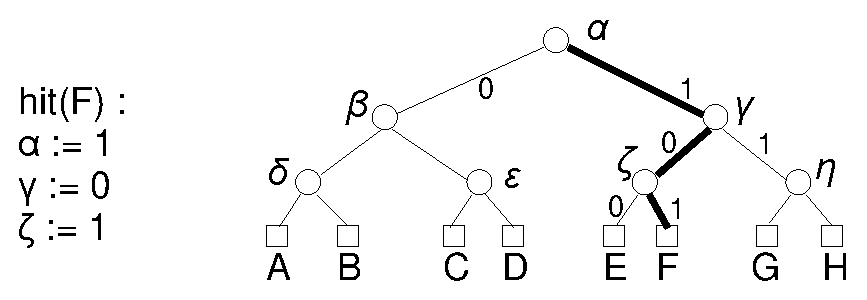
\includegraphics[width=0.7\textwidth]{2.theor/plruhit}\\
  \caption{Попадание для стратегия вытеснения \PseudoLRU
  (8-ассоциативная таблица)}\label{pseudo_lru_hit}
\end{figure}

На основании пометок вершин определяется и листовая вершина вытесняемой строки.
%Вытесняющий тег помещается в дереве на место вытесняемого.
Из корня дерева строится <<вытесняющий путь>> (он будет единственным), он приводит к вытесняемой строке. Начинает <<вытесняющий путь>> строиться из корневой вершины. Далее в <<вытесняющем пути>> исходящая дуга каждой вершины имеет пометку, противоположную пометке этой вершины. Т.е. если вершина помечена цифрой 0, значит дуга пути из этой вершины идет вправо, если вершина помечена цифрой 1 -- влево. Пример того, как определяется вытесняемая строка, показан на рис.~\ref{pseudo_lru_miss}. Цветом показаны пометки нелистовых вершин: черным
вершинам соответствует пометка 1, белым -- 0. В изображенном на рисунке дереве в качестве вытесняемой строки будет выбрана строка D, к которой ведет путь $\alpha-\beta-\varepsilon$.

\begin{figure}[h] \center
  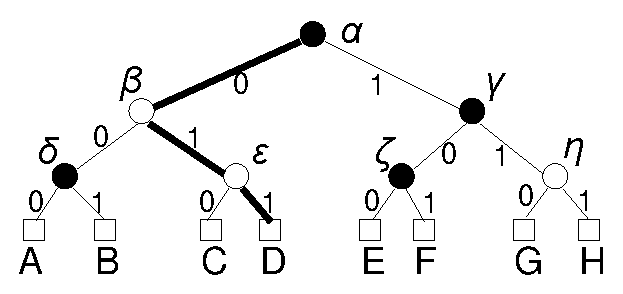
\includegraphics[width=0.5\textwidth]{2.theor/plrumiss}\\
  \caption{Определение вытесняемого элемента для стратегия вытеснения
  \PseudoLRU (8-ассоциативная таблица)}\label{pseudo_lru_miss}
\end{figure}


\subsubsection{Каноническое определение \PseudoLRU на битовой строке}

Для каждого региона хранится битовая строка $\beta$ длины $w{-}1$, где $w$ --
ассоциативность таблицы. Стратегия вытеснения определяется как процесс изменения
бит этой битовой строки.

Во многих книгах приводятся следующее определение стратегии
вытеснения \PseudoLRU для случая
$w=4$~\cite{FundamentalOfComputerOrganizationAndDesign} (в этом
случае для каждого региона выделяется 3 бита $B_1$, $B_2$ и $B_3$):
$$ \left[
  \begin{array}{c|ccc}
          & B_1 & B_2 & B_3 \\ \hline
    \pi_0 & 0 & 0 & \textsf{X} \\
    \pi_1 & 0 & 1 & \textsf{X} \\
    \pi_2 & 1 & \textsf{X} & 0 \\
    \pi_3 & 1 & \textsf{X} & 1 \\
  \end{array}
\right]
$$

Строки в регионе пронумерованы числами от 0 до $w{-}1$. При попадании на строку
региона с номером $i$ задействована строка матрицы, начинающаяся с $\pi_i$. Биты
$\beta$, напротив которых в строке матрицы находится \textsf{X}, не меняются.
Биты $\beta$, напротив которых в $i$'й строке находится число, принимают
значение, равное этому числу.

При промахе надо определить номер вытесняемой строки. Для этого используется
инвертированная форма той же матрицы (если элемент исходной матрицы был равен 0, то в инвертированной он равен 1; если в исходной равен 1, то в инвертированной равен 0; если в исходной равен \textsf{X}, то в инвертированной равен \textsf{X}):
$$
\left[
  \begin{array}{ccc|c}
    B_1 & B_2 & B_3 & \\ \hline
    1 & 1 & \textsf{X} & \rightarrow \pi_0 \\
    1 & 0 & \textsf{X} & \rightarrow \pi_1 \\
    0 & \textsf{X} & 1 & \rightarrow \pi_2 \\
    0 & \textsf{X} & 0 & \rightarrow \pi_3 \\
  \end{array}
\right]
$$

Выбирается строка матрицы, соответствующая текущему состоянию бит $B_1$,
$B_2$ и $B_3$, следующим образом: если напротив бита в строке матрицы находится число, бит
должен быть равен этому числу -- если напротив бита в строке матрицы
находится \textsf{X}, то соответствующий бит может иметь любое значение. Для любого набора значений $(B_1~B_2~B_3)$ подходящая строка матрицы всегда будет существовать и она будет единственной. Эта строка матрицы определяет вытесняемую строку региона.

Изменение $\beta$ обычно демонстрируют на бинарном дереве. Это то же дерево, что и в каноническом определении \PseudoLRU <<на бинарном дереве>>. $\beta$ составляется из пометок вершин дерева, начиная с корня и далее по слоям от левых к правым вершинам <<обходом в ширину>> (см. рис.~\ref{plru_bittree}).

\begin{figure}[h] \center
  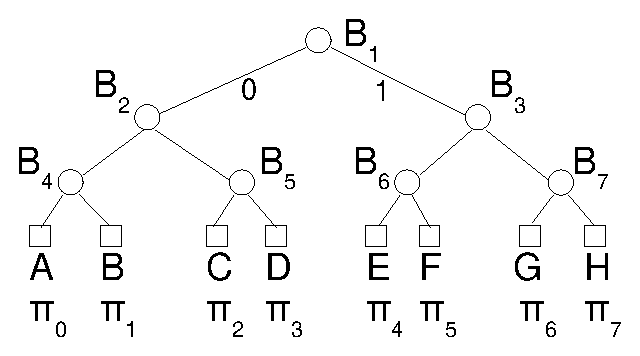
\includegraphics[width=0.5\textwidth]{2.theor/plru}\\
  \caption{Битовая строка в бинарном дереве}\label{plru_bittree}
\end{figure}

Формализованное описание для всех допустимых $w$ в литературе не
приводится. Однако в дальнейшем для формулирования и доказательства
утверждений про стратегию вытеснения \PseudoLRU такое описание будет
необходимо. Для $w=8$ изменение битовой строки будет задаваться следующей матрицей:
$$
\left[
  \begin{array}{c|ccccccc}
          & B_1 & B_2 & B_3 & B_4 & B_5 & B_6 & B_7 \\ \hline
    \pi_0 & 0 & 0 & \textsf{X} & 0 & \textsf{X} & \textsf{X} & \textsf{X} \\
    \pi_1 & 0 & 0 & \textsf{X} & 1 & \textsf{X} & \textsf{X} & \textsf{X} \\
    \pi_2 & 0 & 1 & \textsf{X} & \textsf{X} & 0 & \textsf{X} & \textsf{X} \\
    \pi_3 & 0 & 1 & \textsf{X} & \textsf{X} & 1 & \textsf{X} & \textsf{X} \\
    \pi_4 & 1 & \textsf{X} & 0 & \textsf{X} & \textsf{X} & 0 & \textsf{X} \\
    \pi_5 & 1 & \textsf{X} & 0 & \textsf{X} & \textsf{X} & 1 & \textsf{X} \\
    \pi_6 & 1 & \textsf{X} & 1 & \textsf{X} & \textsf{X} & \textsf{X} & 0 \\
    \pi_7 & 1 & \textsf{X} & 1 & \textsf{X} & \textsf{X} & \textsf{X} & 1 \\
  \end{array}
\right]
$$

Следующее утверждение~\ref{wMinus1PseudoLRU} дает алгоритм
преобразования битовой строки\\ $B_1,~B_2,~...,~B_{w{-}1}$ в результате
обращения в таблицу. В его формулировке будет применяться двоичное
разложение целых неотрицательных чисел от старших бит к младшим. Оно будет обозначаться для целого неотрицательного $x$ как $(x_1~x_2~...~x_n)_2$, где $x_i \in \{0, 1\}$ для $i = 1, 2, ..., n$, такие, что $x = x_n + 2{\cdot}x_{n-1} + 4{\cdot}x_{n-2} + \dots + 2^{n-1}{\cdot}x_1$. Например, 1 = (0 0 1)$_2$, 6 = (1 1 0)$_2$.

Обозначим символом $W$ выражение $\log_2 w$. По определению
стратегии вытеснения \PseudoLRU $W$ будет натуральным числом.

\begin{utv}[$(w{-}1)$-представление стратегии вытеснения
\PseudoLRU]\label{wMinus1PseudoLRU}При попадании по строке региона с номером $i = (i_1~i_2~\dots~i_W)_2$ происходит следующее изменение битовой строки $B_1,
B_2, ..., B_{w{-}1}$:

\parbox{0.3\textwidth}{
  $$ \begin{array}{l}
  B_{k_1} := i_1 \\
  B_{k_2} := i_2 \\
  B_{k_3} := i_3 \\
  ...\\
  B_{k_W} := i_W \\
  \end{array}$$
} \vline
\parbox{0.7\textwidth}{
  $$ \begin{array}{l}
  k_1 = (1)_2 \\
  k_2 = (1~i_1)_2 \\
  k_3 = (1~i_1~i_2)_2 \\
  ...\\
  k_W = (1~i_1~i_2~\dots~i_{W{-}1})_2 \\
  \end{array} $$
}
\\[1cm]

При промахе номер вытесняемой строки региона $j = (j_1~j_2~\dots~j_W)_2$ определяется следующим образом:

\parbox{0.3\textwidth}{
  $$ \begin{array}{l}
  i_1 = \neg B_{k_1} \\
  i_2 = \neg B_{k_2} \\
  i_3 = \neg B_{k_3} \\
  ...\\
  i_W = \neg B_{k_W} \\
  \end{array}$$
} \vline
\parbox{0.7\textwidth}{
  $$ \begin{array}{l}
  k_1 = (1)_2 \\
  k_2 = (1~\neg B_{k_1})_2 \\
  k_3 = (1~\neg B_{k_1}~\neg B_{k_2})_2 \\
  ...\\
  k_W = (1~\neg B_{k_1}~\neg B_{k_2}\dots\neg B_{k_{W{-}1}})_2 \\
  \end{array} $$
}
\\[0.5cm]

Кроме того при промахе делается такое же преобразование бит $B_1$, $B_2$, ..., $B_{w{-}1}$, как и в случае попадания на строку с номером $j$.
\end{utv}

Прямой проверкой нетрудно убедиться, что это утверждение верно для $w$ = 4 и 8.

\subsubsection{Определение \PseudoLRU на ветвях бинарного
дерева}\label{sec:PseudoLRUonBranches}

Здесь будет показано, как из канонических определений \PseudoLRU
получить формулировку \PseudoLRU с точки зрения одной строки региона~\cite{my_lomonosov_2010}
(в канонических определениях рассматривается весь регион целиком и
для него формулируются правила работы с последовательностью бит $B_1,
B_2, ..., B_{w{-}1}$ или пометками вершин бинарного дерева). Описываемое в этом разделе определение \PseudoLRU ранее не встречалось в литературе.

Сначала этот переход покажем в частном случае, на примере $w=4$. Первый шаг --- это
смена <<состояния>>: вместо последовательности бит $B_1, B_2, ...,
B_{w-1}$ будем рассматривать последовательность векторов бит
$\beta_0,~\beta_1,~\dots,~\beta_{w-1}$, каждый $\beta_i$ --- это вектор из $W$ бит. Каждый $\beta_i$ соответствует $i$'й листовой вершине бинарного дерева (см. рисунок~\ref{fig:plru_def_step1}). Попадание
меняет теперь атрибуты не внутренних вершин дерева $(B_1~B_2~B_3)$, а листовых $(\beta_0~...~\beta_3)$.
Каждый $\beta_i$ будет представляться списком длины $W$, обозначающим путь от
корня дерева к $i$'й листовой вершине: $\beta_0$ соответствует
($B_1$ $B_2$), $\beta_1$ соответствует ($B_1$ $\neg B_2$), $\beta_2$
соответствует ($\neg B_1$ $B_3$) и $\beta_3$ соответствует ($\neg
B_1$ $ \neg B_3$).\\[0.5cm]

\begin{figure}[h]
\parbox{0.2\textwidth}{ \centering
  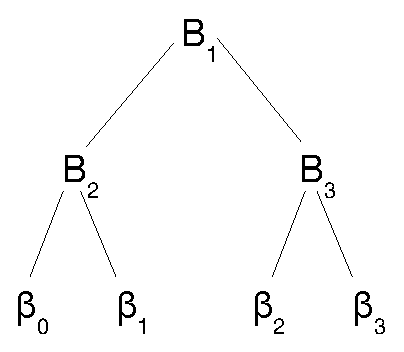
\includegraphics[width=0.2\textwidth]{1.review/btree}
}
\parbox{0.25\textwidth}{
$$ \left[
  \begin{array}{c|ccc}
          & B_1 & B_2 & B_3 \\ \hline
    \pi_0 & 0 & 0 & \textsf{X} \\
    \pi_1 & 0 & 1 & \textsf{X} \\
    \pi_2 & 1 & \textsf{X} & 0 \\
    \pi_3 & 1 & \textsf{X} & 1 \\
  \end{array}
\right]
$$
} $\stackrel{1}{\longrightarrow}$ %\vline
\parbox{0.4\textwidth}{
$$ \left[
  \begin{array}{c|cccc}
          & \beta_0 & \beta_1 & \beta_2 & \beta_3 \\ \hline
    \pi_0 & (0~0) & (0~1) & (1~\textsf{X}) & (1~\textsf{X}) \\
    \pi_1 & (0~1) & (0~0) & (1~\textsf{X}) & (1~\textsf{X}) \\
    \pi_2 & (1~\textsf{X}) & (1~\textsf{X}) & (0~0) & (0~1) \\
    \pi_3 & (1~\textsf{X}) & (1~\textsf{X}) & (0~1) & (0~0) \\
  \end{array}
\right]
$$
}
\caption{Смена состояния}\label{fig:plru_def_step1}
\end{figure}

Заметим, что получилась симметричная матрица. На пересечении $\pi_i$
и $\beta_j$ располагается вектор, задающий изменение $\beta_j$ (вектора в $j$'й
листовой вершине дерева) при попадании по строке региона, соответствующей $i$'й листовой вершине дерева. Назовем позицию $i \oplus j$ \emph{относительной позицией}
$i$ относительно $j$. Рассмотрим отдельно каждый столбец
получившейся матрицы (на рисунке~\ref{fig:plru_def_step2} до стрелки) и упорядочим строки столбцов в порядке увеличения относительных позиций (на рисунке~\ref{fig:plru_def_step2} после стрелки).

\begin{figure}[h]
\parbox{0.2\textwidth}{
$$ \left[
  \begin{array}{c|c}
          & \beta_0 \\ \hline
    \pi_0 & (0~0) \\
    \pi_1 & (0~1) \\
    \pi_2 & (1~\textsf{X}) \\
    \pi_3 & (1~\textsf{X}) \\
  \end{array}
\right]
$$
}\parbox{0.2\textwidth}{
$$ \left[
  \begin{array}{c|c}
          & \beta_1 \\ \hline
    \pi_0 & (0~1) \\
    \pi_1 & (0~0) \\
    \pi_2 & (1~\textsf{X}) \\
    \pi_3 & (1~\textsf{X}) \\
  \end{array}
\right]
$$
}\parbox{0.2\textwidth}{
$$ \left[
  \begin{array}{c|c}
          & \beta_2 \\ \hline
    \pi_0 & (1~\textsf{X}) \\
    \pi_1 & (1~\textsf{X}) \\
    \pi_2 & (0~0) \\
    \pi_3 & (0~1) \\
  \end{array}
\right]
$$
}\parbox{0.2\textwidth}{
$$ \left[
  \begin{array}{c|c}
          & \beta_3 \\ \hline
    \pi_0 & (1~\textsf{X}) \\
    \pi_1 & (1~\textsf{X}) \\
    \pi_2 & (0~1) \\
    \pi_3 & (0~0) \\
  \end{array}
\right]
$$
} $\stackrel{2}{\stackrel{\longrightarrow}{\pi^i_j \equiv \pi_{i
\oplus j}}}$

\parbox{0.24\textwidth}{
$$ \left[
  \begin{array}{c|c}
          & \beta_0 \\ \hline
    \pi^0_0 \equiv \pi_0 & (0~0) \\
    \pi^0_1 \equiv \pi_1 & (0~1) \\
    \pi^0_2 \equiv \pi_2 & (1~\textsf{X}) \\
    \pi^0_3 \equiv \pi_3 & (1~\textsf{X}) \\
  \end{array}
\right]
$$
}\parbox{0.24\textwidth}{
$$ \left[
  \begin{array}{c|c}
          & \beta_1 \\ \hline
    \pi^1_0 \equiv \pi_1 & (0~0) \\
    \pi^1_1 \equiv \pi_0 & (0~1) \\
    \pi^1_2 \equiv \pi_3 & (1~\textsf{X}) \\
    \pi^1_3 \equiv \pi_2 & (1~\textsf{X}) \\
  \end{array}
\right]
$$
}\parbox{0.24\textwidth}{
$$ \left[
  \begin{array}{c|c}
          & \beta_2 \\ \hline
    \pi^2_0 \equiv \pi_2 & (0~0) \\
    \pi^2_1 \equiv \pi_3 & (0~1) \\
    \pi^2_2 \equiv \pi_0 & (1~\textsf{X}) \\
    \pi^2_3 \equiv \pi_1 & (1~\textsf{X}) \\
  \end{array}
\right]
$$
}\parbox{0.24\textwidth}{
$$ \left[
  \begin{array}{c|c}
          & \beta_3 \\ \hline
    \pi^3_0 \equiv \pi_3 & (0~0) \\
    \pi^3_1 \equiv \pi_2 & (0~1) \\
    \pi^3_2 \equiv \pi_1 & (1~\textsf{X}) \\
    \pi^3_3 \equiv \pi_0 & (1~\textsf{X}) \\
  \end{array}
\right]
$$
}
\caption{Нумерация относительными позициями}\label{fig:plru_def_step2}
\end{figure}

После перехода к относительным позициям ($\pi^i_j$ -- это позиция
$\pi_j$ относительно $\pi_i$, т.е. $\pi_{i \oplus j}$) все столбцы получились одинаковыми.
Иными словами, \emph{алгоритм изменения порядка строк региона согласно стратегии
вытеснения \PseudoLRU на относительных позициях инвариантен
относительно абсолютной позиции вытесняемой строки}. Следующая теорема
формально доказывает этот факт.

Будем называть \emph{\PseudoLRU-ветвью позиции $i$} вектор
$(B_{k_1}^{\sigma_1}~B_{k_2}^{\sigma_2}~\dots~B_{k_W}^{\sigma_W})$,
в котором $k_1 = (1)_2, \sigma_1 = \neg i_1, \sigma_j = \neg i_j$, $k_j = (1~i_1~i_2~\dots~i_{j-1})_2$, $j = 2, 3, \dots, W$, $i = (i_1~i_2~\dots~i_W)_2$. Степени определены стандартным образом: $B^1 \equiv B, B^0 \equiv \neg B$. Например, \PseudoLRU-ветвью позиции 0 есть $(B_1~B_2~B_4~...)$. Каждой строке региона (т.е. каждой позиции строк региона) соответствует своя \PseudoLRU-ветвь. Каждое обращение изменяет все ветви некоторым образом, который не зависит от абсолютной позиции, а зависит от относительной:

\begin{theorem}[Инвариантность преобразования \PseudoLRU-ветвей относительными
позициями]\label{thm_pseudoLRU_invariant} \PseudoLRUInvariant
\end{theorem}
Доказательство теоремы приведено в приложении~\ref{sec:proofs}.

Доказанный факт позволяет сформулировать определение стратегии
вытеснения \PseudoLRU, сфокусированное не на изменении атрибутов строк всего
региона,
а на изменении атрибутов одной строки. На этом определении
будут базироваться применения предлагаемых методов генерации
ограничений для стратегии вытеснения \PseudoLRU.

\begin{utv}[формулировка \PseudoLRU на ветвях бинарного дерева]
Сопоставим некоторой произвольной строке региона вектор длины $W$. Каждое обращение к этой строке региона делает её вектор равным (0 0 ... 0). Строка региона является вытесняемой, если её вектор равен (1 1 ... 1).
Влияние других обращений определяется относительной позицией их
строки региона относительно позиции данной строки региона. Если относительная позиция
принадлежит области $[\frac{w}{2^k},~\frac{w}{2^{k-1}}), k =
1,2,...,W$, то первые $k{-}1$ элементов битового вектора становятся равными
0, $k$'й элемент вектора становится равным 1, остальные элементы
вектора не меняются. Если относительная позиция равна 0, то все элементы вектора становятся равными 0.
\end{utv}

Битовый вектор длины $W$ будет соответствовать пути из корня бинарного
дерева в листовую вершину, соответствующую данной строке региона.
Удобно представлять процесс изменения элементов бинарного вектора  в виде их
\emph{перекрашивания}. Про элементы битового вектора, равные 0,
будем говорить, что они покрашены в \emph{белый} цвет, а элементы вектора, равные 1, --- в\emph{черный}.

Говоря в терминах бинарного дерева из канонических определений \PseudoLRU, каждое обращение в регион изменяет пометки в нелистовых вершинах дерева. Каждой листовой вершине соответствует единственный в нее путь из корня дерева (та самая <<ветвь>>). Вершина дерева, входящая в ветвь, с точки зрения этой ветви будет <<белой>>, если пометка этой вершины совпадает с направлением дуги дерева из этой вершины. входящей в ветвь, <<черной>> --- если не совпадает. Вытесняется та строка региона, путь к которой полностью состоит из несоответствующих дуг по каноническим определениям, т.е. из черных вершин по новому определению. На рисунке~\ref{recolor}
изображен процесс перекрашивания ветви, ведущей в А, под действием
попадания в C (для сокращения показана только ветвь в А без
остальной части дерева). Так как путь из корня в C совпадает из
верхних двух вершин, то они перекрашиваются в белый цвет. Дуга из
третьей вершины пути в С не совпадает с дугой пути в А, поэтому
третья вершина перекрашивается в черный цвет. Остальные вершины
ветви остаются без изменений.

\begin{figure}[h] \center
  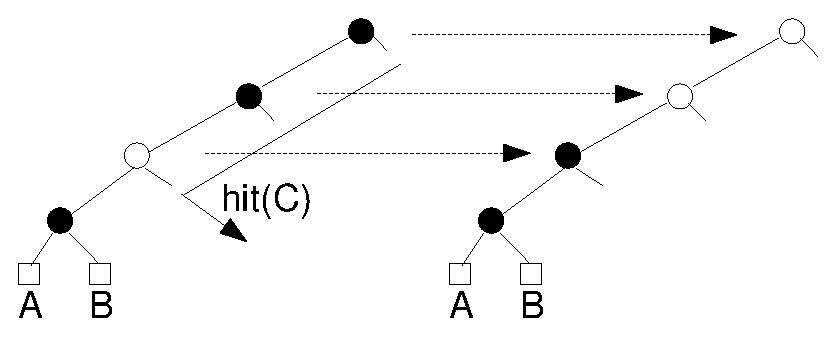
\includegraphics[width=0.8\textwidth]{1.review/recolor}\\
  \caption{Перекрашивание ветви в А}\label{recolor}
\end{figure}


Определение стратегии вытеснения \PseudoLRU на ветвях дерева
является связующим звеном между каноническим определением (например,
на битовой строке) и определением с помощью таблицы вытеснения,
поскольку ветвь -- это и есть двоичное разложение позиции, которая меняется точно так же, как и позиция в перестановке согласно таблице вытеснения.


%%%%%%%%%%%%%%%%%%%%%%%%%%%%%%%%%%%%%%%%%%%%%%%%%%%%%%%%%%%%%%%%%%%%

\section{Метод полезных обращений для записи стратегии вытеснения в виде ограничений}\label{sec:usefulness_functions}

%{\footnotesize В разделе рассматривается метод составления ограничений для
%описания стратегии вытеснения, для которой удается определить функционал
%вытеснения. Стратегия вытеснения описывается ограничением сверху на количество \emph{полезных} инструкций (т.е. помогающих вытеснению).
%В разделе приведены определения полезных инструкций и способы составления ограничений для трех
%наиболее часто используемых в микропроцессорах стратегий вытеснения -- \LRU, \FIFO и \PseudoLRU. Освещается понятие \emph{монотонного функционала вытеснения}, который является залогом более
%простой системы ограничений.}

В данном разделе процесс вытеснения будет представляться как изменение  системы функций, отображающих ключи в целые числа. Каждое обращение в таблицу изменяет значения функций по всем ключам\footnote{это напоминает изменение операций в рамках машин абстрактного состояния Ю.Гуревича~\cite{ASM}}. Пример процесса изменения значения функции для некоторого ключа изображен на рисунке~\ref{fig:graphic}.

\begin{figure}[h] \center
  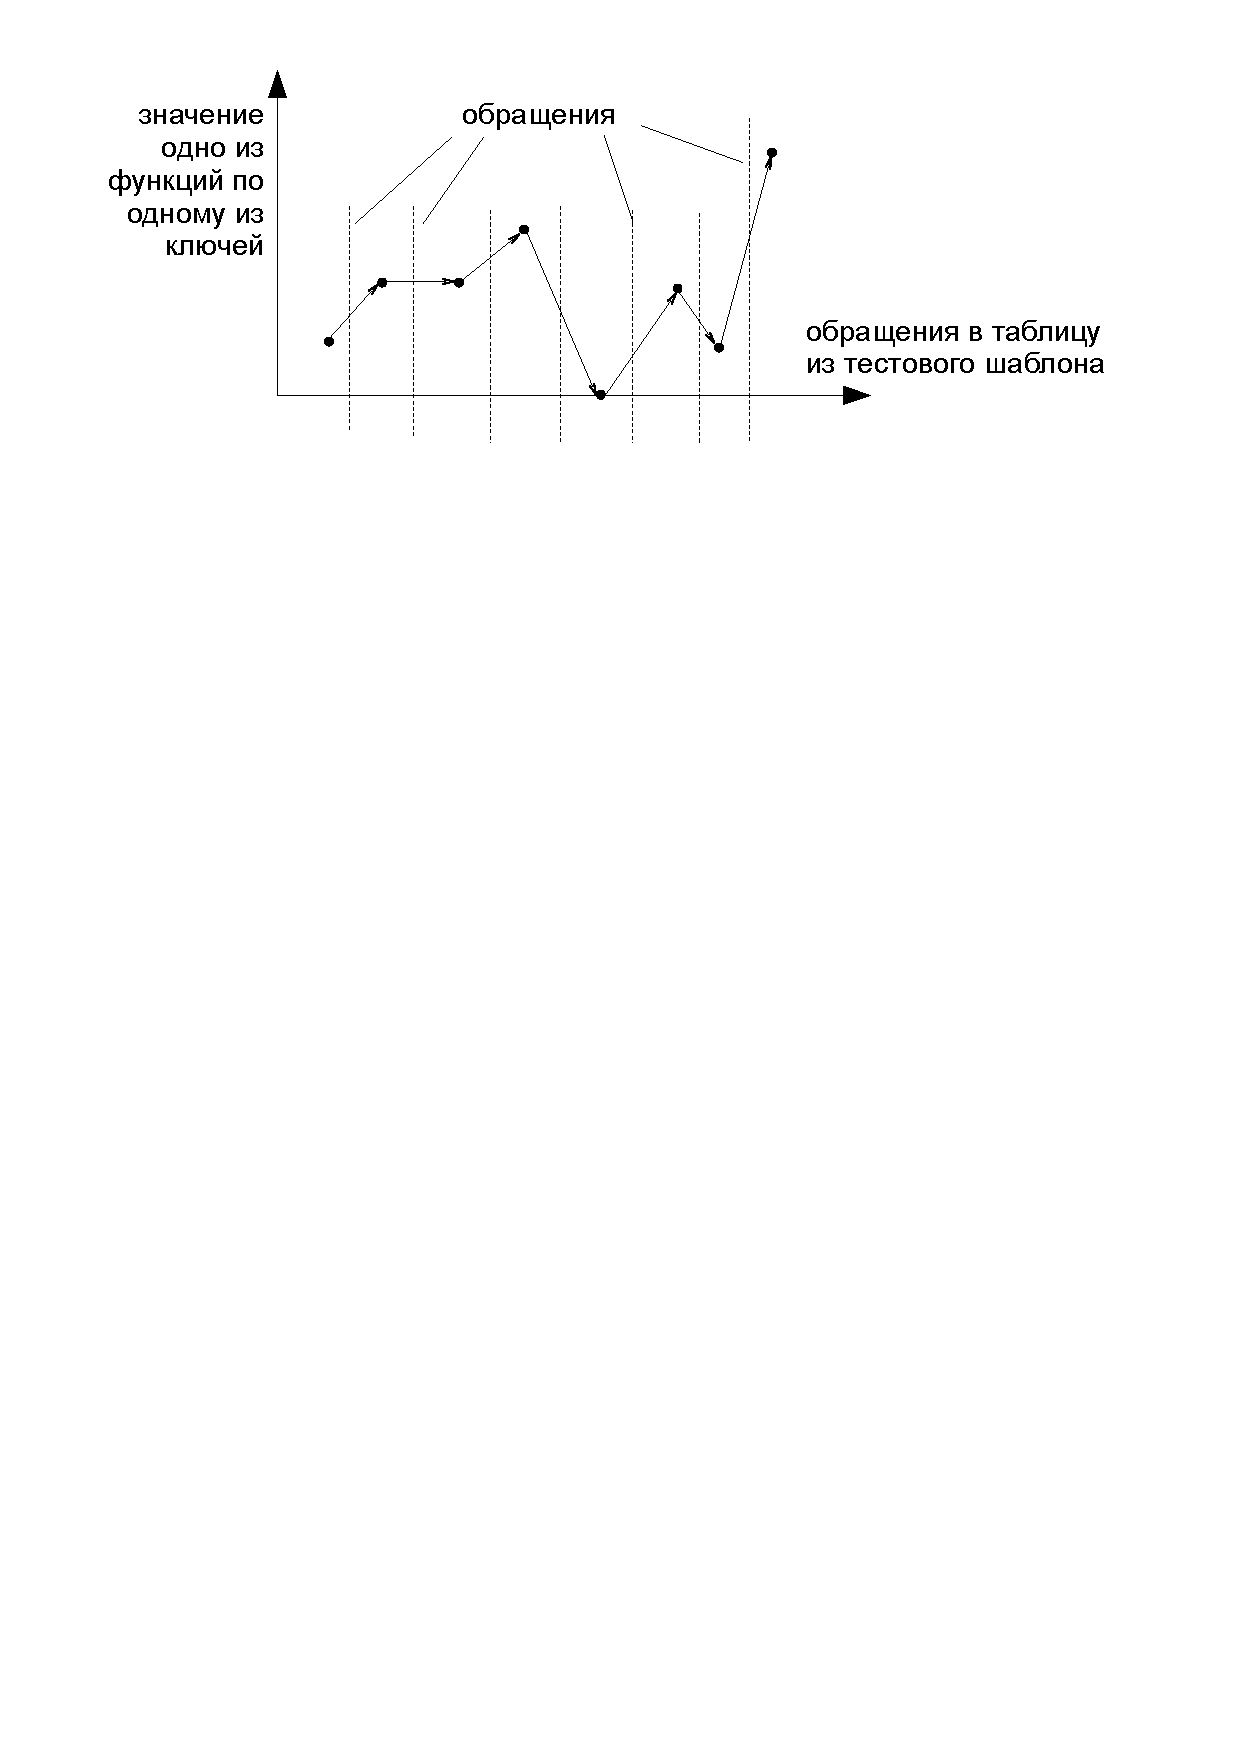
\includegraphics[width=0.7\textwidth]{2.theor/graphic}\\
  \caption{К определению стратегии вытеснения}\label{fig:graphic}
\end{figure}

Говоря формально, пусть $\alpha, \beta, \dots, \gamma$ --- одноместные функции,
отображающие ключи в целые числа. Для каждого обращения определены функции
изменения значений функций $\alpha, \beta, \dots, \gamma$ (если не сказано иное, будет предполагаться, что обращения осуществляются в один и тот же регион):
$$\parbox{2.5cm}{in-parallel\\forall keys x~}\left|\begin{array}{l}
\alpha(x) := A_I(k, \alpha, \beta, \dots, \gamma)\\
\beta(x) := B_I(k, \alpha, \beta, \dots, \gamma)\\
\dots\\
\gamma(x) := C_I(k, \alpha, \beta, \dots, \gamma)\\
\end{array}\right.
$$

Обновления значений функций $\alpha, \beta, \dots, \gamma$ выполняются одновременно. $I$ --- обращение в таблицу, $k$ --- ключ в этом обращении. Функции $A_I$, $B_I$, \dots, $C_I$ отражают влияние обращения по некоторому ключу на другой произвольный ключ. $x$ --- это ключ, за которым <<следим>> и условия вытеснения которого нас интересуют, а $k$ ---это ключ в очередном обращении из тестового шаблона.
Возможны следующие случаи (в качестве $x$ рассматривается произвольный ключ, не
обязательно <<находящийся>> в регионе):
\begin{itemize}
    \item в результате обращения по ключу $k$ ключ $x$ <<попадает>> в регион (т.е. в регион добавляется строка с ключом $x$);
    \item в результате обращения по ключу $k$ ключ $x$ <<вытесняется>> из региона (т.е. из региона удаляется строка с ключом $x$);
    \item в результате обращения по ключу $k$ <<состояние>> ключа $x$ в регионе не меняется.
\end{itemize}

%Этим ситуациям как раз и ставятся в соответствие классы значений функций $\alpha, \beta, \dots, \gamma$, а функции $A_I$, $B_I$, \dots, $C_I$ осуществляют переход между этими классами. Тем самым стратегия вытеснения будет описана в виде изменения таких <<счетчиков>> $\alpha, \beta, \dots, \gamma$.

%Формально это правило выражается следующим образом.
Будем называть функцию
$\alpha$, отображающую ключи в целые числа, \emph{функционалом вытеснения} для заданной стратегии вытеснения, если одновременно выполнены следующие свойства:
\begin{enumerate}
  \item существуют константы $\alpha_{min}$ и $\alpha_{max}$ такие, что
$\alpha_{min} \leqslant \alpha_{max}$;
  \item для любого ключа $x$ $\alpha_{min} \leqslant \alpha(x) \leqslant
\alpha_{max}$ тогда и только тогда, когда $x$ находится в регионе по определению
стратегии вытеснения (т.е. <<был помещен>> в регион и до сих пор не вытеснен);
  \item для любого ключа $k$ $A_I(k, \alpha,\beta,\dots,\gamma) (k) =
\alpha_{min}$;
  \item $\exists! \varphi: \mbox{~ключ~} \times \mathds{Z}^{n} \times \mbox{~ключ~} \times \mathds{Z}^{n} \rightarrow
\mathds{Z}$, где $n$ --- количество функций во множестве
$\{\alpha,\beta,\dots,\gamma\}$, такая, что для любого ключа $x$ $$A_I(k,
\alpha,\beta,\dots,\gamma)(x) \equiv \varphi(k, \alpha(k), \beta(k), \dots,
\gamma(k), x, \alpha(x), \beta(x), \dots, \gamma(x))$$ иными словами, в функции
изменения функционала вытеснения разрешается обращаться только к $k$ и тому ключу,
для которого определяется функционал вытеснения;
  \item $\exists!$ ключ $x^* : \alpha(x^*) = \alpha_{max}$;
  \item перед любым неуспешным обращением $\alpha(x^*) =
\alpha_{max}$ тогда и только тогда, когда $x^*$ есть <<вытесняемый>> ключ по
определению стратегии вытеснения (т.е. строка с ключом $x^*$ является
вытесняемой при данном обращении по определению стратегии вытеснения);
\end{enumerate}

Пример функционала вытеснения: $\alpha$ --- счетчик количества обращений к строке
для стратегии вытеснения \LRU. Обращение по тому же ключу делает $\alpha$
равным 1, по другому ключу --- увеличивает $\alpha$ на единицу. Вытесняемым
считается ключ, чей счетчик равен $w$ --- количеству строк в регионе. Проверим
определение функционала вытеснения:
\begin{enumerate}
    \item $\alpha_{min}$ = 1, $\alpha_{max}$ = $w$, $1 \leqslant w$;
    \item верно, что счетчик больше $w$ тогда и только тогда, когда $x$ не
находится в регионе; в противном случае, было бы возможно подряд успешно обратиться к
большему числу строк, чем хранится в регионе;
    \item по условию обращение по тому же ключу делает $\alpha$ равным 1, что
и есть $A_I(x;...)(x) = 1$;
    \item изменение одного счетчика производится независимо от изменений других счетчиков (хотя, конечно, все счетчики изменяются одновременно);
    \item такой $x^*$ существует, ибо в противном случае было бы возможно подряд успешно обратиться к большему числу строк, чем хранится в регионе; такой $x^*$ единственный, поскольку каждое обращение меняет каждый счетчик и в минимальное значение $\alpha$ изменяется лишь по единственному ключу.
\end{enumerate}

Пусть для стратегии вытеснения сформулирован функционал вытеснения. Будем называть
обращение по некоторому ключу \emph{полезным для вытеснения} ключа
$x$ (или просто, \emph{полезным}), если оно монотонно увеличивает функционал вытеснения по
ключу $x$ до максимального значения (см. рис.~\ref{useful}).\\

\begin{figure}[h] \center
  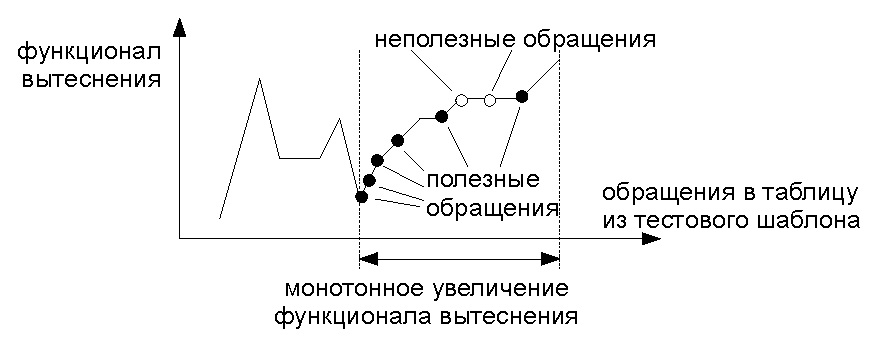
\includegraphics[width=0.6\textwidth]{2.theor/useful}\\
  \caption{К определению полезных обращений}\label{useful}
\end{figure}

Тогда вытеснение будет происходить в том случае, когда количество
полезных обращений превысит некоторое константное количество.
И вытеснение не будет происходить, если это количество не превысит некоторой константной верхней границы.

\emph{Формулой полезного обращения} будем называть предикат от вытесняемого ключа $k$ и региона $R$ и ключей и регионов предыдущих обращений, при которых это обращение будет полезным для вытеснения ключа $k$ из региона $R$.

Тем самым ограничение (constraint) <<быть вытесненным>> представимо в виде
ограничения сверху на <<сумму>> формул полезных обращений по всем предыдущим обращениям: $\sum_{i=1}^n [u_x(k_i)] < N$, где $u_x(k_i)$ -- формула полезного обращения по ключу $k_i$ для ключа $x$ в полностью ассоциативной таблице, для остальных таблиц будут указываться регионы обращений: $u_{x,r}(k_i, r_i)$.

Формулы полезных обращений, как и функционалы вытеснения, не являются единственными. Например, для стратегии вытеснения \LRU возможны следующие две различные формулы полезных обращений (далее для одной из них будет формально показано, что она действительно задает полезные обращения) (формулы приведены для случая полностью ассоциативной таблицы):
\begin{itemize}
  \item $u_x(x_i) \equiv (x \notin \{x_i, x_{i+1}, ..., x_n\} \wedge
\bigwedge\limits_{j=1}^{i-1} (x \in \{x_j, x_{j+1}, ..., x_{i-1}\} \vee x_j
\neq x_i))$ -- обращение считается полезным, если оно расположена после
последнего обращения к $x$ и с того момента является первым обращением к своему
ключу; нетрудно заметить, что это в чистом виде определение \LRU, изображенное на рисунке~\ref{fig:lru1}: обращение по ключу $x_j$, который расположен после ключа $x$, передвигает $x$ к концу вектора, за концом происходит вытеснение; первые обращения по ключам после последнего обращения к $x$ -- это и есть именно те обращения, где $x$ сдвигается к концу; иначе говоря, полезное обращение сдвигает $x$ к концу, приближая его к вытеснению;
  \item $u_x(x_i) \equiv (x \notin \{x_i, x_{i+1}, ..., x_n\} \wedge x_i \notin
\{x_{i+1}, x_{i+2}, ..., x_n\})$ -- обращение считается полезным, если оно
расположено после последнего обращения к $x$ и является последним обращением к
своему ключу перед финальным обращением к $x$; т.е. в таблице хранятся некоторые ключи, есть некоторый ключ $x$, есть последовательность других обращений (их
ключи обозначены как  $x_i$, ..., $x_n$), полезными будут лишь последние к ним обращения (среди $x_i$, ..., $x_n$ могут быть равные), т.е. все полезные обращения вместе образуют (по разу) все различные ключи.
\end{itemize}

Тем самым, метод полезных обращений состоит в следующем:
\begin{enumerate}
  \item выделить функционал вытеснения $\alpha$;
  \item выделить определение полезной инструкции;
  \item записать формулу полезного обращения $u_{x,r}(x_i, r_i)$ для обращения с ключом $x$ и регионом $r$;
  \item определить $\alpha_{max}$;
  \item составить ограничение для свойства <<$x$ вытеснен>> в виде
$\sum\limits_{i=1}^n u_{x,r}(x_i, r_i) > \alpha_{max}$ и для свойства <<$x$ не
вытеснен>> в виде $\sum\limits_{i=1}^n u_{x,r}(x_i,r_i) \leqslant \alpha_{max}$.
\end{enumerate}

Ключевой вопрос при применении метода полезных обращений --- это выбор
функционала вытеснения. От него в том числе будет зависеть сложность функции
полезности и генерируемых ограничений.

 Функционал вытеснения может быть получен из таблицы вытеснения
(policy table). А именно, если вытеснение происходит с позиции с максимальным
номером (т.е. в последней строке отсутствует число $w{-}1$), а в результате
попадания ключ переносится в самое начало (т.е. второй столбец имеет вид (0 1 2
... $w{-}1$ $m$)$^T$ ). Тогда $\alpha$ --- это позиция ключа в перестановке,
$\alpha_{min}$ = 0, $\alpha_{max} = w{-}1$. Этими свойствами, например, обладают
таблицы вытеснения \LRU (см.рис.~\ref{fig:PolicyTableLRU8}) и
\PseudoLRU~\cite{policy_tables}.

%В отличие от метода диапазонов вытеснения при использовании функций полезности не происходит выделение участка тестового шаблона, непосредственно влияющего на вытеснение. Считается, что это влияние начинается с момента появления строки в таблице. Другое дело, что одни инструкции влияют на ее вытеснение (это и есть <<полезные>> инструкции), а другие -- нет.


\subsection{Метод полезных обращений для стратегии вытеснения \LRU}

\LRU (Least Recently Used) --- это стратегия вытеснения,
определяющая вытесняемые данные как наименее используемые. Она
эффективна для алгоритмов, обладающих свойством локальности данных,
т.е. чаще использующих те данные, к которым недавно происходило
обращение. Эта стратегия используется, например, в микропроцессорах
архитектуры MIPS~\cite{mips64II}.

Стратегия вытеснения \LRU обычно определяется с использованием
счетчиков обращений. Для каждой строки таблицы
вводится счетчик обращений к ней. Каждое обращение увеличивает
счетчик. Счетчик вытесняющей строки на единицу больше максимального счетчика невытесняемых строк. Вытесняемой в регионе будет строка с минимальным счетчиком его строк.
%Поскольку границы значений счетчика неизвестны, формулирование
%функционала вытеснения на основе счетчика провести сложно.

Другой способ описания \LRU основан на введении порядка на строках региона (т.е.
регион представляется вектором строк). После каждой инструкции элементы этого вектора переупорядочиваются, \emph{переставляются}, согласно следующим правилам (см.рис.~\ref{fig:lru1}):
\begin{itemize}
\item при попадании соответствующая строка перемещается в начало, строки, которые расположены левее этой, сдвигаются на одну позицию вправо;
\item при промахе вытесняется последняя строка, в начало вставляется вытесняющая.
\end{itemize}

\begin{figure}[h] \center
  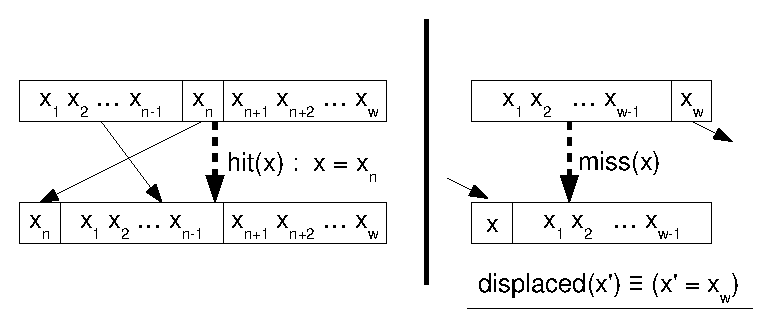
\includegraphics[width=0.6\textwidth]{2.theor/lru1}\\
  \caption{Стратегия вытеснения \LRU (w --- ассоциативность) на
перестановках}\label{fig:lru1}
\end{figure}

Позиция строки, ее индекс, в таком векторе ограничена, единственна, ее изменение допускает представление, независимое от других ключей. Тем самым \emph{<<позиция>> ключа является функционалом вытеснения}.

Функция изменения этого функционала выглядит следующим образом:\\

\parbox{0.5\textwidth}{ \tt
$A_{\mbox{hit}}(k, \alpha)(x) \equiv$\\
if $\alpha(x) > w$ then $\alpha(x)$\\
elsif $\alpha(k) > \alpha(x)$ then $\alpha(x)+1$\\
elsif $\alpha(k) = \alpha(x)$ then $1$\\
else $\alpha(x)$ endif%
}\parbox{0.5\textwidth}{\tt
$A_{\mbox{miss}}(k, \alpha)(x) \equiv$\\
if $k = x$ then $1$\\
elsif $\alpha(x) > w$ then $\alpha(x)$\\
else $\alpha(x) + 1$ endif}\\

Полезным будет считаться обращение, увеличивающее позицию, т.е.
переставляющее соответствующий ключ к концу. Такими обращениями являются все
промахи (поскольку они вытесняют последнюю строку вектора с передвижением всех остальных на одну позицию к концу, т.е. будет передвинута и строка с ключом $x$) и
попадания к строкам, находившимся ближе к концу, чем $x$ (потому как при попадании они передвинутся в самое начало, а все строки от начала и до них сдвинутся на одну
позицию к концу, в том числе и $x$).

Осталось выразить эту идею в виде ограничений~\cite{my_ewdts_2009}.
Учет полезных обращений начинается уже в инициализирующей последовательности,
тем самым необходимо будет сформулировать формулы полезных обращений и для
инициализирующих обращений.

Следующая теорема описывает функцию полезности для \LRU ($m$ --- количество
инициализирующих инструкций):

\begin{theorem}[Выражение свойства <<быть вытесненным>> для \LRU]\label{correct_mirror_LRU} \LRUusefuls
\end{theorem}

\begin{proof}
По определению стратегии вытеснения \LRU <<$k$ не вытеснен из региона $R$ согласно определению на перестановках>> эквивалентно тому, что после последнего обращения к $k$ в $R$ происходит не более $w$ обращений по различным ключам в регион $R$. Несложно убедиться, что это количество выражается следующей формулой: $$|\{s_i| R = R(s_i) \wedge s \notin \{s_i, ..., s_{m+n}\}\}|$$
Однако это же число можно записать другим образом, чтобы исключить повторения одинаковых $s_i$:
$$|\{s_i| R = R(s_i) \wedge s \notin \{s_i, ..., s_{m+n}\} \wedge s_i \notin \{s_{i+1}, ..., s_{m+n}\}\}|$$

Ввиду конечности последовательности $\langle s_i, ..., s_{m+n}\rangle$ в нем всегда найдется последнее вхождение $s_i$ --- множество последних вхождений всех элементов списка равно множеству всех элементов списка.

Представленная мощность множества и есть требуемая сумма.
\end{proof}

Из теоремы~\ref{correct_mirror_LRU} следует система ограничений для
описания обращений по ключу $k_i$ в регион $R_i$ согласно методу полезных обращений для \LRU: \begin{itemize}
\item для hit($k_i, R_i$):
$$
\left\{\begin{array}{l} (k_i||R_i) \in \{(t_1||r_1), ..., (t_m||r_m), (k_1||R_1),
..., (k_{i-1}||R_{i-1})\}\\
\sum\limits_{j=1}^m [u_{k_i,R_i}(t_j||r_j)] + \sum\limits_{j=1}^{i-1} [u_{k_i,R_i}(k_j||R_j)] < w\\
\{(t_1||r_1), ..., (t_m||r_m)\} - \mbox{все разные}\\
\end{array} \right.
$$
\item для miss($k_i, R_i$):
$$
\left\{\begin{array}{l} (k_i||R_i) \in \{(t_1||r_1), ..., (t_m||r_m), (k_1||R_1),
..., (k_{i-1}||R_{i-1})\}\\
\sum\limits_{i=1}^m [u_{k_i,R_i}(t_j||r_j)] + \sum\limits_{j=1}^{i-1} [u_{k_i,R_i}(k_j||R_j)]
\geqslant w\\
\{(t_1||r_1), ..., (t_m||r_m)\} - \mbox{все разные}\\
\end{array} \right.
$$
\end{itemize}


%Для этого удобно использовать утверждение~\ref{hit_miss_human}. Символом
%$\lambda_\delta$ будет обозначаться элемент начального
%состояния таблицы с индексом $\delta$ по порядку \LRU, $1 \leqslant \delta \leqslant w$. Индекс 1 обозначает самый молодой элемент, индекс $w$ обозначает самый старый элемент.
%
%Применение полезностей эффективно в том случае, когда домен имеет
%небольшой размер. В этом случае можно перебрать все элементы
%домена (это и будут $\lambda_\delta$) и составить для них свои
%полезности, причем для каждого элемента будет известен индекс по
%порядку \LRU ($\delta$). Ограничение, описывающее стратегию
%вытеснения, будет при этом иметь вид дизъюнкции по элементам домена.
%
%Если вытесняемый элемент был в начальном состоянии (пусть это
%$\lambda_\delta$) и к нему не было обращений, то для его вытеснения
%необходимо $w-\delta + 1$ полезных инструкций, потому что столько
%раз надо подвинуть элемент с индексом $\delta$ в \LRU-списке в
%сторону к концу (к элементам с индексом $w$), чтобы он вышел за
%границу списка (иными словами, чтобы он был вытеснен).
%
%Если вытесняемый элемент был в начальном состоянии и к нему было
%обращение, то для его вытеснения необходимо $w$ инструкций, так как
%во время обращения элемент был поставлен в самое начало \LRU-списка.
%То же справедливо для внесенных в кэширующий буфер новых тегсетов --
%чтобы их вытеснить, надо так же $w$ полезных инструкций, чтобы
%переместить их к концу \LRU-списка.
%
%В таблице~\ref{hit_miss_table} приведены все функции полезности для
%кэш-попаданий и кэш-промахов. Доказательство корректности приведенных
% в ней формул (т.е. доказательство того, что эти формулы действительно
% описывают \LRU) важны, но не представляют самостоятельного результата.
%Поэтому они были вынесены за пределы основной части диссертации и
%находятся в приложении~\ref{sec:proofs}.

В некоторых случаях количество ограничений удается сократить, используя следующую эвристику для ограничения вида $\sum_{i=1}^n a_i \leqslant C$:
\begin{itemize}
    \item если $C > n$, то его не включать в конъюнкцию;
    \item если $C < 0$, то вся конъюнкция с этим ограничением несовместна;
    \item если $C = 0$, то его сразу расписать в конъюнкцию ограничений
$a_i = 0$ для каждого $i$ от 1 до $n$;
    \item если $C = n$, то его сразу расписать в конъюнкцию ограничений
$a_i = 1$ для каждого $i$ от 1 до $n$.
\end{itemize}

Аналогично с ограничениями вида $\sum_{i=1}^n a_i \geqslant C$.


\subsection{Метод полезных обращений для стратегии вытеснения \FIFO}

\FIFO (First-In First-Out) -- это стратегия вытеснения, определяющая
вытесняемые данные согласно принципу очереди FIFO. Например, в
микропроцессоре PowerPC 970FX вытеснение из небольшого буфера,
хранящего последние преобразованные эффективные адреса в физические,
D-ERAT, происходит согласно \FIFO~\cite{PowerPC970FXUserManual}.

Стратегия \FIFO допускает описание на основе порядка на строках
региона (т.е. регион представляется вектором строк-элементов). После каждого
обращения строки вектора переупорядочиваются, \emph{перставляются}, согласно следующим правилам
(см.рис.~\ref{fifo1}):
\begin{itemize}
\item при попадании порядок строк не меняется;
\item при промахе вытесняется последняя строка, в начало вставляется вытесняющая строка.
\end{itemize}

\begin{figure}[h] \center
  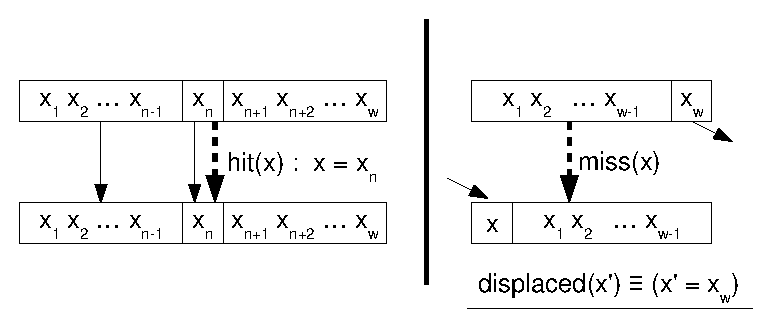
\includegraphics[width=0.6\textwidth]{2.theor/fifo1}\\
  \caption{Стратегия вытеснения \FIFO (w --- ассоциативность
таблицы)}\label{fifo1}
\end{figure}

Отличие от \LRU лишь в том, что при \FIFO не происходит перестановки
строк при возникновении попадания. Поэтому таблица
вытеснения~\cite{policy_tables} для стратегии вытеснения \FIFO будет
выглядеть так, как изображено на рисунке~\ref{fifo_policy_table}.

\begin{figure}[h]
$$
  \left[
    \begin{array}{c|cccccc}
      \pi_0 & 0 & 1 & 2 & 3 & \dots & w{-}1 \\
      \pi_1 & 0 & 1 & 2 & 3 & \dots & w{-}1 \\
      \pi_2 & 0 & 1 & 2 & 3 & \dots & w{-}1 \\
      \vdots &  &  &  & & & \\
      \pi_{w-1} & 0 & 1 & 2 & 3 & \dots & w{-}1 \\
      \pi_m & m & 0 & 1 & 2 & \dots & w{-}2 \\
    \end{array}
  \right]
$$
\caption{Таблица вытеснения для \FIFO}\label{fifo_policy_table}
\end{figure}

Формулы полезных обращений для \FIFO будем строить также на основе уже сформулированных и обоснованных формул для \LRU.

%Кроме того все инструкции с попаданиями, поскольку они не влияют на вытеснение, можно вообще исключить из ограничений.

Таким образом система уравнений для описания обращений по ключу $k$ в регион $R$
согласно методу полезных обращений для \FIFO выглядит следующим образом:
\begin{itemize}
\item для hit($k_i, R_i$):
$$
\left\{\begin{array}{l} (k_i||R_i) \in \{(t_1||r_1), ..., (t_m||r_m), (k_1||R_1), ..., (k_{i-1}||R_{i-1})\}\\
\sum\limits_{j=1}^m [u_{k_i,R_i}(t_j||r_j)] + \sum\limits_{j=1..{i-1}:(k_j,R_j)\mbox{~--miss}} [u_{k_i,R_i}(k_j||R_j)] < w\\
\{(t_1||r_1), ..., (t_m||r_m)\} - \mbox{все разные}\\
\end{array} \right.
$$
\item для miss($k_i, R_i$):
$$
\left\{\begin{array}{l} (k_i||R_i) \in \{(t_1||r_1), ..., (t_m||r_m), (k_1||R_1), ..., (k_{i-1}||R_{i-1})\}\\
\sum\limits_{j=1}^m [u_{k_i,R_i}(t_j||r_j)] + \sum\limits_{j=1..{i-1}:(k_j,R_j)\mbox{~--miss}} [u_{k_i,R_i}(k_j||R_j)] \geqslant w\\
\{(t_1||r_1), ..., (t_m||r_m)\} - \mbox{все разные}\\
\end{array} \right.
$$
\end{itemize}

$$u_{k_i,R_i}(s_j) \equiv ((k_i||R_i) \notin \{s_j, ..., s_{m+n}\} \wedge R_i = R(s_j) \wedge s_j \notin\{s_{j+1},..., s_{m+n}\})$$
$s \equiv \langle (t_1||r_1), ..., (t_m||r_m), (k_1||R_1), ..., (k_n||R_n)\rangle$, $R(s_i)$ --- вторая компонента $s_i$ (регион).


\subsection{Метод полезных обращений для стратегии вытеснения \PseudoLRU}

Для определения функционала вытеснения воспользуемся определением\\\PseudoLRU <<на ветвях бинарного дерева>> (см. раздел~\ref{sec:PseudoLRUonBranches}). А именно, определение того, вытеснен ли ключ $k$ в регионе $R$, будет вестись на основе атрибутов вершин пути от корня дерева к  листу, соответствующему $k$. Эти вершины могут быть белыми (им сопоставлено число 0) или чёрными (им сопоставлено число 1). Обращение по другому ключу $k_i$ в этом же регионе перекрашивает некоторые вершины этого пути. А именно, при следовании от корня к листу сначала часть вершин перекрашивается в белый цвет, затем одна вершина красится в черный цвет, остальные вершины не перекрашиваются. Если $k_i = k$, то все вершины ветви красятся в белый цвет.

  \begin{figure}[h] \center
  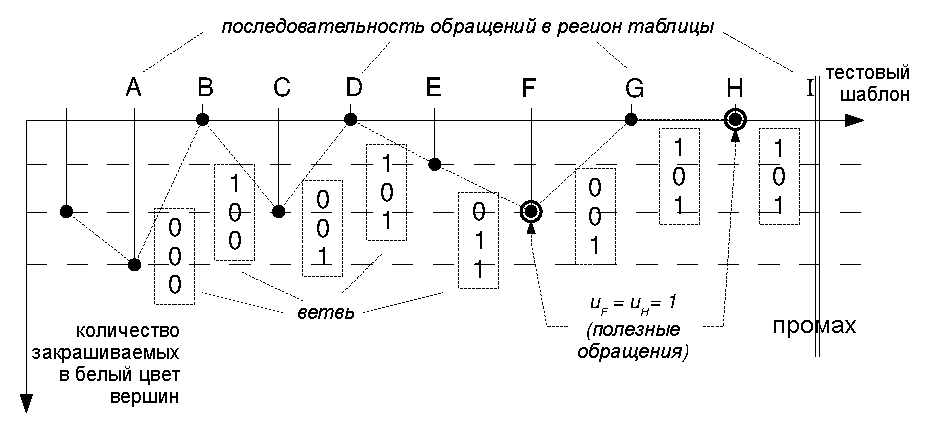
\includegraphics[width=\textwidth]{2.theor/plru_usefl_exmp}
  \caption{Перекрашивание ветви последовательностью обращений}\label{fig:plru_exmp_vytesn}
  \end{figure}

На рисунке~\ref{fig:plru_exmp_vytesn} изображен пример процесса перекрашивания для \\8-ассоциативной таблицы. В этом примере рассматривается ветвь, ведущая в строку, к которой происходит обращение А. После обращения к своей же строке вся ветвь становится белой: линия из А в В помечена (0 0 0)$^T$. Чем <<глубже>> по оси ординат происходит обращение, тем <<глубже>> становится белой ветвь (значение по оси ординат означает количество подряд вершин ветви, начиная с первой (самой верхней в векторах на рисунке), которые становятся равными нулю, а следующая за ней вершина, если она существует, становится равной единице, остальные вершины не меняются). Обращение В самое <<мелкое>>, оно лишь меняет первую вершину ветви, делая ее чёрной. Следующее обращение, С, перекрашивает 2 вершины в белый цвет (в том числе и ту вершину, которую только что обращение В покрасило в чёрный цвет) и 1 вершину в чёрный цвет. И так далее.

Обратим внимание на обращения F и H. Вершины, которые они закрашивают в чёрный цвет, сохраняют свой цвет до промаха, в котором будет определяться, вытеснять ли данную строку. Это происходит потому, что все следующие обращения происходят с закрашиванием меньшего числа вершин, чем F и H. В качестве функционала вытеснения рассмотрим количество таких обращений, как F и H, т.е. таких, после которых обращения закрашивают меньшее число вершин: самое большое число таких вершин есть длина ветви, самое малое - ноль (обращение А), изменений одной ветви определяется без отсылок к другим ветвям, вытеснение происходит тогда и только тогда, когда количество чёрных вершин равно длине ветви.

%Например, представленный на рисунке~\ref{fig:plru-useful} шаблон успевает
% покрасить 5 вершин ветви в черный цвет.
%
%\begin{figure}[t] \center
%  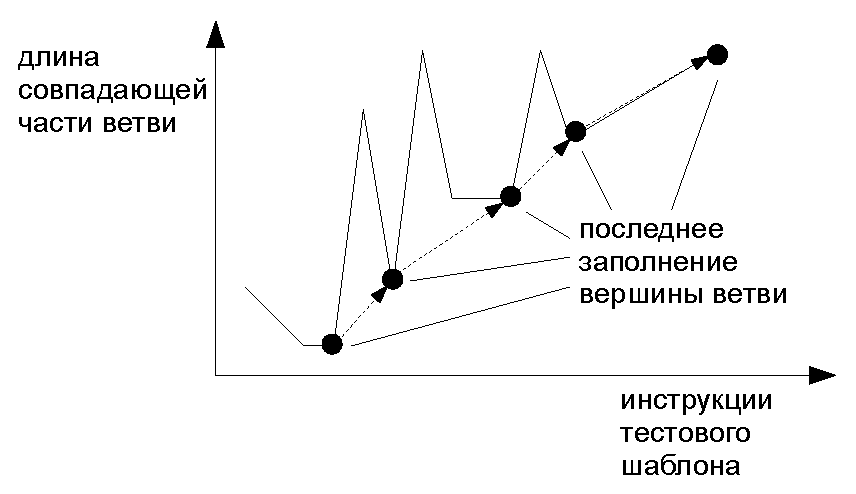
\includegraphics[width=0.6\textwidth]{2.theor/plru-useful}\\
%  \caption{Заполнение ветви черными вершинами в стратегии вытеснения
%  \PseudoLRU}\label{fig:plru-useful}
%\end{figure}

\begin{utv}
Обращение $I$ считается полезным в случае стратегии вытеснения \PseudoLRU, если все последующие обращения (до промаха, в котором вся ветвь будет чёрной) затрагивают только те вершины ветви, которые расположены выше вершины, перекрашиваемой инструкцией $I$ в черный цвет.
\end{utv}

Для вытеснения нужно не менее $\log_2 w$ полезных обращений (длина ветви). Далее выражение $\log_2 w$ будет обозначаться буквой $W$.

%Отличие этого функционала вытеснения от функционала для \LRU является \emph{немонотонность}. Это означает, что полезные инструкции надо считать для каждого промаха заново ---
%инструкции между двумя соседними промахами могут <<забелить>>
%несколько вершин ветви, что уменьшит функционал вытеснения
%(см.рис.~\ref{nonmonotonic}). Метрика для \LRU является монотонной,
%потому что инструкции между промахами не могут уменьшить функционал вытеснения -- либо не меняют, либо увеличивают ее, сдвигая ключ к концу вектора \LRU (см. рис.~\ref{monotonic}).
%
%%Таким образом, ограничение, описывающее стратегию вытеснения
%%\PseudoLRU, будет представлено дизъюнкцией ограничений по всем
%%предыдущим кэш-промахам.
%
%\begin{figure}[h] \center
%  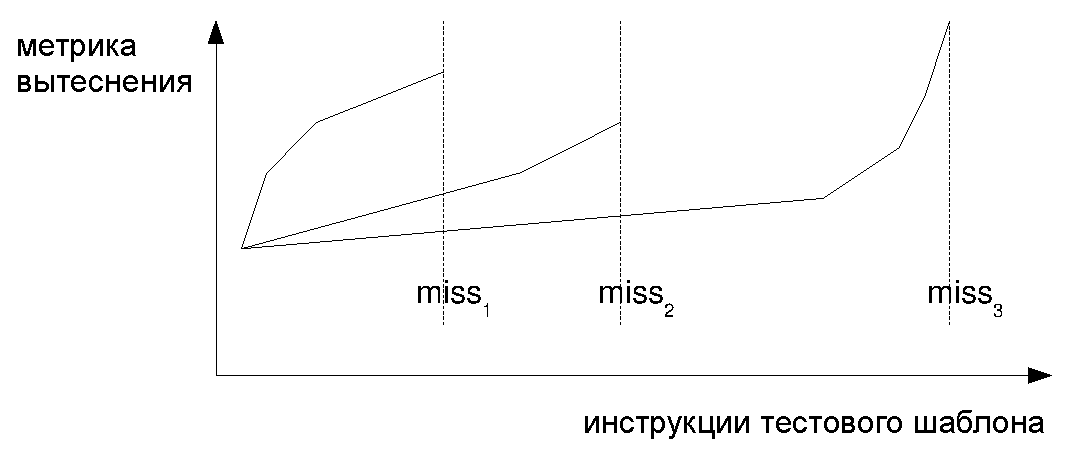
\includegraphics[width=0.6\textwidth]{2.theor/nonmonotonic}\\
%  \caption{Немонотонный функционал вытеснения}\label{nonmonotonic}
%\end{figure}
%
%\begin{figure}[h] \center
%  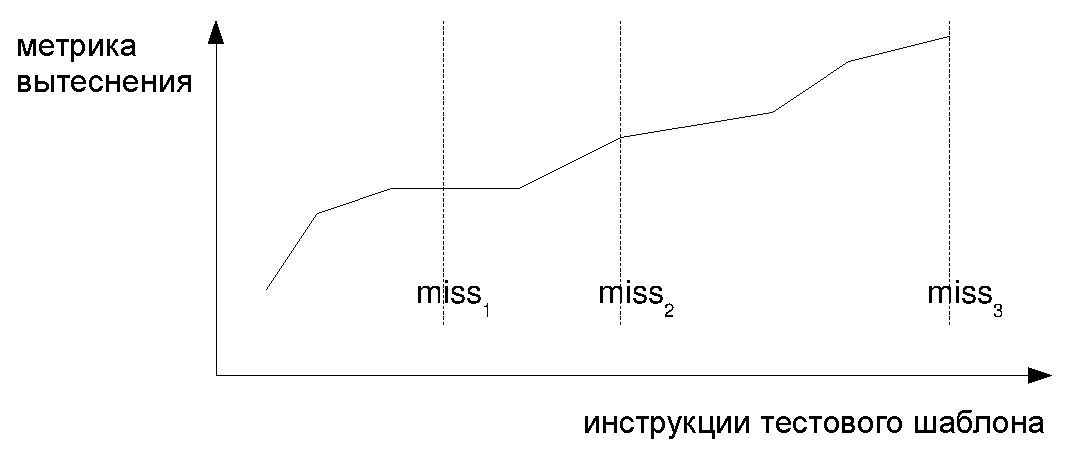
\includegraphics[width=0.6\textwidth]{2.theor/monotonic}\\
%  \caption{Монотонный функционал вытеснения}\label{monotonic}
%\end{figure}

Осталось записать формулу полезного обращения для \PseudoLRU в виде ограничений. Определимся с набором переменных. Каждому обращению в таблицу будут соответствовать следующие переменные:
\begin{itemize}
  \item ключ $k_i$;
  \item регион $R_i$;
  \item позиция $\pi_i$ (определение см. в разделе~\ref{sec:PseudoLRUonBranches}), $\pi_i \in \{0..w{-}1\}$;
  \item позиция $\pi'_i$ в момент последнего обращения перед данным (только для неинициализирующих обращений).
\end{itemize}

Обращение по ключу $k_i$ в регион $R_i$ на позицию $\pi_i$ будет полезным для вытеснения ключа $k_{n+1}$ в регионе $R_{n+1}$ ($i < n+1$) с позицией в момент последнего обращения $\pi'_{n+1}$, если выполнены все следующие условия (ниже будет доказано, что это определение соответствует стратегии вытеснения \PseudoLRU):
\begin{enumerate}
  \item <<$i$'е>> обращение происходит после последнего обращения к $k_{n+1}$ в $R_{n+1}$ перед $(n+1)$'м обращением;
  \item <<$i$'е>> обращение происходит в тот же регион, что и $R_{n+1}$;
  \item <<$i$'e>> обращение происходит до ближайшего повторного обращения на позиции $\pi'_{n+1}$;
  \item все обращения после <<$i$'го>> до ближайшего повторного обращения на позиции $\pi'_{n+1}$ просходит без закрашивания той вершины, которую красит <<$i$'e>> обращение.
\end{enumerate}

В момент последнего обращения по ключу $k_{n+1}$ в $R_{n+1}$ ветвь к нему становится целиком белой и начинается процесс вытеснения. Последующие инструкции перекрашивают эту ветвь до тех пор, пока не встретится обращение с промахом на той же позиции, которая была в момент последнего обращения к $k_{n+1}$ в $R_{n+1}$. К этому моменту вся ветвь должна стать чёрной, а после этого обращения ветвь вновь становится белой, но эта ветвь уже относится к другому ключу (тому, который вытеснил $k_{n+1}$).

Поясню этот момент с другой стороны. Рассматривая успешность очередного обращения к некоторому ключу, ищем ближайшее предыдущее обращение к тому же ключу (обращение А на рисунке~\ref{fig:plru_exmp_vytesn}). Обращения, идущие после этого <<предыдущего>>, либо должны вытеснить соответствующий ключ (если речь идёт о неуспешном обращении), либо не должны вытеснить (если --- об успешном). Если среди этих обращений не встречается обращение по той же позиции, что и в момент <<предыдущего>> обращения, то вытеснение не произойдет (т.к. в противном случае в этом обращении могло произойти бы вытеснение по определению \PseudoLRU). Если же обращение встречается (обращение I на рисунке~\ref{fig:plru_exmp_vytesn}), то к его моменту вся ветвь должна успеть стать полностью чёрной.

Переменные $\pi_i$ для позиций обладают собственными ограничениями, не зависящими от успешности обращений по ним. А именно, позиции --- это битовые строки длины $W$, идентифицирующие ключи: если позиции двух обращений совпадают и между ними нет промахов по этой позиции, то ключи должны совпадать, если же позиции различаются, то и ключи должны различаться (обозначим $t_i$ и $r_i$ --- ключи и регионы инициализирующих обращений, $k_i$ и $R_i$ --- ключи и регионы в обращениях из тестового шаблона, обозначим $s \equiv \langle (t_1||r_1), ..., (t_m||r_m), (k_1||R_1), ..., (k_n||R_n)\rangle$):

для каждой пары обращений $i$ и $j$ ($j$'е --- после $i$'го)
\begin{itemize}
    \item если $S_j$ = hit, то $$(\pi_i||R(s_i) = \pi_j||R(s_j)~\wedge$$ $$\pi_i||R(s_i) \notin \{\pi_{m_1}||R(s_{m_1}), \pi_{m_2}||R(s_{m_2}), \dots, \pi_{m_n}||R(s_{m_n})\}) \rightarrow s_i = s_j$$
    \item если $S_j$ = miss, то $$(\pi_i||R(s_i) = \pi_j||R(s_j)~\wedge$$ $$\pi_i||R(s_i) \notin \{\pi_{m_1}||R(s_{m_1}), \pi_{m_2}||R(s_{m_2}), \dots, \pi_{m_n}||R(s_{m_n})\}) \rightarrow s_i \neq s_j$$
\end{itemize}
где $(\pi_{m_1},R(s_{m_1})), (\pi_{m_2},R(s_{m_2})), \dots, (\pi_{m_n},R(s_{m_n}))$ --- позиции и регионы неуспешных обращений,
расположенных между $i$'м и $j$'м обращениями. В качестве $i$'го обращения также надо рассмотреть и инициализирующие обращения.

%% это "перевернутые"позиции! у них чем ближе к листу, тем дальше от левой границы в битовом представлении

И, наконец, определение для $\pi'_i$ в виде ограничений. Если $S_i$ = hit, то  $\pi'_i$ --- позиция в том обращении, где в последний раз встретился ключ $k_i$ в регионе $R_i$:
$$
\begin{array}{l}
\texttt{(ite~} ((k_i||R_i) = (k_{i-1}||R_{i-1})) ~~ (\pi'_i = \pi_{i-1})\\
\texttt{(ite~} ((k_i||R_i) = (k_{i-2}||R_{i-2})) ~~ (\pi'_i = \pi_{i-2})\\
... ~(\pi'_i = 0)\texttt{)))...)}\\
\end{array}
$$

Подформула $\pi'_i = 0$ не оказывает влияния, если $(k_i||R_i) \in \{(k_{i-1}||R_{i-1}),$ $(k_{i-2}||R_{i-2}), ... \}$, а так и будет

Если $S_i = $ miss, то кроме того, что $\pi'_i$ --- позиция последнего вхождения ключа $k_i$ в регионе $R_i$, надо убедиться, что та же позиция $\pi'_i$ встречается после последнего обращения к $k_i$ в $R_i$ на неуспешном обращении ( $\{\pi_i, ..., \pi_j\}_m$ обозначает подмножество множества позиций от $i$'го до $j$'го обращения из неуспешных обращений):
$$
\begin{array}{l}
\texttt{(ite~} ((k_i||R_i) = (k_{i-1}||R_{i-1})) ~~ (\pi'_i = \pi_{i-1})\\
\texttt{(ite~} ((k_i||R_i) = (k_{i-2}||R_{i-2})) ~~ (\pi'_i = \pi_{i-2} \wedge \pi'_i \in \{\pi_{i-1}\}_m)\\
\texttt{(ite~} ((k_i||R_i) = (k_{i-3}||R_{i-3})) ~~ (\pi'_i = \pi_{i-3} \wedge \pi'_i \in \{\pi_{i-1}, \pi_{i-2}\}_m)\\
... ~(\pi'_i = 0)\texttt{)))...)}\\
\end{array}
$$

Переходим непосредственно к записи формулы полезного обращения. Запишем каждое условие этого определения в виде ограничений ( $k_{n+1}$ и $R_{n+1}$ --- ключ и регион, по отношению к которым определяется вытеснение, $s \equiv \langle (t_1||r_1), ..., (t_m||r_m), (k_1||R_1), ..., (k_n||R_n)\rangle$ --- предыдущие обращения (ключи и регионы), $\sigma \equiv \langle (\tau_1||r_1), ..., (\tau_m||r_m), (\pi_1||R_1), ..., (\pi_n||R_n)\rangle$ --- предыдущие обращения (позиции и регионы), $i$ --- номер обращения, для которого записывается формула полезного обращения, $R(s_i)$ --- вторая компонента $s_i$, $R(\sigma_i)$ --- вторая компонента $\sigma_i$, $\pi(\sigma_i)$ --- первая компонента $\sigma_i$) :
\begin{enumerate}
    \item $(k_{n+1}||R_{n+1}) \notin \{s_i, s_{i+1}, ...,  s_{m+n}\}$ -- $i$'е обращение происходит после последнего обращения к $k_{n+1}$ в $R_{n+1}$;
    \item $R_{n+1} = R(s_i)$ -- обращение происходит в тот же регион;
    \item $(\pi'_{n+1}||R_{n+1}) \in \{\sigma_i, \sigma_{i+1}, ..., \sigma_{m+n}\}$ -- обращение происходит до ближайшего повторного обращения на ту же позицию;
    \item $\bigwedge\limits_{j = i+1}^n (((\pi'_{n+1}||R_{n+1}) \notin \{\sigma_i, \sigma_{i+1}, ..., \sigma_j\}~\wedge~R(\sigma_i) = R(\sigma_j)) \rightarrow P(\pi(\sigma_i) \oplus \pi'_{n+1}, \pi(\sigma_j) \oplus \pi'_{n+1}))$ --- полезные инструкции должны закрашивать больше белых вершин, чем закрашивают все последующие инструкции;  предикат $P$ для пары векторов $\delta_i$ и $\delta_j$ (<<относительных позиций>> --- см. раздел~\ref{sec:PseudoLRUonBranches}) истинен тогда и только тогда, когда количество старших нулевых бит у $\delta_i$ больше количества старших нулевых бит у $\delta_j$, иными словами, только и только тогда, когда существует целое $k$ такое, что $\delta_i < 2^k \leqslant \delta_j$ (см.рис.~\ref{fig:bits}); из леммы~\ref{QuantorElimination} (ее формулировка и доказательство находятся в приложении~\ref{sec:proofs}) следует, что этот предикат обладает бескванторной эквивалентной формой: $P(\delta_i, \delta_j) \equiv (\delta_j > \delta_i~~\wedge~~\delta_j \oplus \delta_i > \delta_i)$, сравнения беззнаковые.
\end{enumerate}

\begin{figure}[h] \center
  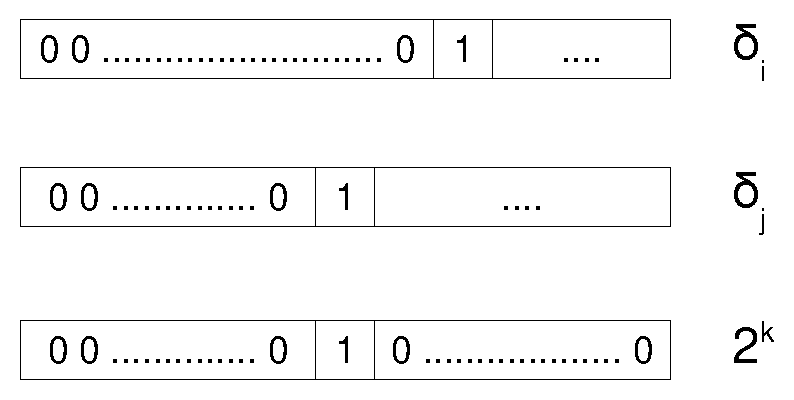
\includegraphics[width=0.4\textwidth]{2.theor/bits}\\
  \caption{Перекрашивание и битовые строки}\label{fig:bits}
\end{figure}

Итак, система ограничений для описания обращений по ключу $k_i$ в регион $R_i$ согласно методу полезных обращений для \PseudoLRU:
\begin{itemize}
\item для hit($k_i, R_i$):
$$
\left\{\begin{array}{l}
(k_i||R_i) \in \{(t_1||r_1), ..., (t_m||r_m), (k_1||R_1), ..., (k_{i-1}||R_{i-1})\}\\
\{(t_1||r_1), ..., (t_m||r_m)\} - \mbox{все разные}\\
\sum\limits_{j=1}^m [u_{k_i,R_i,\pi'_i}(t_j||r_j)] + \sum\limits_{j=1}^{i-1} [u_{k_i,R_i,\pi'_i}(k_j||R_j)] < W\\
\end{array} \right.
$$
\item для miss($k_i, R_i$):
$$
\left\{\begin{array}{l}
(k_i||R_i) \in \{(t_1||r_1), ..., (t_m||r_m), (k_1||R_1), ..., (k_{i-1}||R_{i-1})\}\\
\{(t_1||r_1), ..., (t_m||r_m)\} - \mbox{все разные}\\
\sum\limits_{j=1}^m [u_{k_i,R_i,\pi'_i}(t_j||r_j)] + \sum\limits_{j=1}^{i-1} [u_{k_i,R_i,\pi'_i}(k_j||R_j)] \geqslant W\\
\end{array} \right.
$$
\end{itemize}

$$u_{k_i,R_i,\pi'_i} (s_j)  \equiv \left\{\begin{array}{l}
(k_i||R_i) \notin \{s_j, s_{j+1}, ..., s_{m+n}\}\\
R_i = R(s_j)\\
(\pi'_i||R_i) \in \{(\pi_j||R_j), (\pi_{j+1} || R_{j+1}), ..., (\pi_{m+n}||R_{m+n})\}\\
\bigwedge\limits_{l = j+1}^{m+n} (R_j = R_l ~\wedge~(\pi'_i||R_i) \notin \{(\pi_j||R_j), (\pi_{j+1}||R_{j+1}), ..., (\pi_l||R_l)\}\\
 \hspace{2cm} \rightarrow P(\pi_j \oplus \pi'_i, \pi_l \oplus \pi'_i))\\
\end{array}\right.
$$
$$s \equiv \langle (t_1,r_1), (t_2,r_2), ..., (t_m,r_m), (k_1, R_1), ..., (k_n,R_n) \rangle$$
$$R(s_i) \mbox{~--- вторая компонента~} s_i$$
$$P(x, y) \equiv (y > x~~\wedge~~x \oplus y > x)$$


%Таблица~\ref{plru_table} содержит ограничения для разных случаев
%кэш-попаданий и кэш-промахов (см. утверждение~\ref{hit_miss_human}).
%В каждое из них включается ограничение на количество полезных
%инструкций согласно предлагаемой методике использования функций
%полезности. Полезности считаются относительно некоторого кэш-промаха
%(для их перебора используется сокращение $x_m : \mbox{miss}$).

В приложении~\ref{sec:proofs} доказана теорема~\ref{PLRUusefulThm} эквивалентности этих формул определению стратегии вытеснения \PseudoLRU.

Немного изменив формулу для $\pi'_i$, можно упростить ограничения \textbf{для}\\ \textbf{успешных} обращений. А именно, определив $\pi'_i$ так:

$$
\begin{array}{l}
\texttt{(ite~} (s_i = s_{i-1}) ~~ (\pi'_i = \pi_{i-1})\\
\texttt{(ite~} (s_i = s_{i-2}) ~~ (\pi'_i = \pi_{i-2} \wedge \pi'_i \neq \pi_{i-1})\\
...\\
\texttt{(ite~} (s_i = s_j) ~~ (\pi'_i = \pi_j \wedge \pi'_i \notin \{\pi_{j+1}, ..., \pi_{i-1}\})\\
... \texttt{~true )))...)}\\
\end{array}
$$

для hit($k_i, R_i$) будет достаточно таких ограничений:
$$
\left\{\begin{array}{l}
(k_i||R_i) \in \{(t_1||r_1), ..., (t_m||r_m), (k_1||R_1), ..., (k_{i-1}||R_{i-1})\}\\
\{(t_1||r_1), ..., (t_m||r_m)\} - \mbox{все разные}\\
\end{array} \right.
$$
т.е. ограничение на сумму будет автоматически выполнено. Этот факт следует из того, что о возможности вытеснения можно вести речь там, где встречается хотя бы одно неуспешное обращение на позиции $\pi'_i$. Если же позиция $\pi'_i$ не встречается после последнего обращения к ключу $k_i$, то и вытеснение произведено не будет (в формулах полезных обращений третье условие ложно для всех $s_j$, значит, количество полезных обращений равно равно 0, что означает невытеснение).

\subsection{Разрешение ограничений, описывающих стратегии вытеснения}

Ограничения, которые предлагается строить для описания количества полезных обращений, являются \emph{ограничениями мощности} (cardinality constraints). Это
ограничения вида $C_1 \leqslant \sum_{i=1}^n a_i \leqslant C_2$, где $C_1, C_2$
-- неотрицательные целые числа, а $a_i$ принимают значения 0 или
1~\cite{smt_debugging, PiskacK08, KuncakR07,
Revesz05}. Речь идет об ограничении размера некоторого множества
элементов, заданного с помощью характеристической функции.
В~\cite{smt_debugging} проведено исследование способов записи
ограничений мощности и показано, что от формы записи зависит
эффективность разрешения этих ограничений. Одна из таких форм рассматривает ограничения
мощности как компактную форму записи уравнения
вида $\bigvee_{C_1 \leqslant C \leqslant C_2} \sum_{i=1}^n a_i = C$,
где равенство есть
\begin{itemize}
\item тождественная ложь, если $C < 0$ или $C > n$;
\item конъюнкция $\bigwedge_{1\leqslant i\leqslant n} (a_i = 0)$,
если $C = 0$;
\item дизъюнкция по всевозможным выборкам индексов $i_1, ..., i_C$, где
для каждого индекса $i_k$ справедливы свойства $1 \leqslant i_k
\leqslant n$ и $i_k < i_{k+1}$, конъюнкций $\bigwedge_{i_k} (a_{i_k}
= 1)$, если $1 \leqslant C \leqslant n$.
\end{itemize}

В диссертации не ставилась задача исследования способов разрешения ограничений
мощности (с целью выбора наиболее эффективного способа их представления). Вместо
этого были использованы
имеющиеся инструменты разрешения ограничений мощности~\cite{Z3, Yices}. Для
записи оставшихся формул был использован язык битовых строк, для разрешения
ограничений над которым существуют эффективные SMT-инструменты (например,
Z3~\cite{Z3}).

%После устранения ограничений мощности в формуле остаются только
%ограничения на конечные множества тегсетов: принадлежности и
%непринадлежности тега конечному множеству тегсетов и равенства и
%неравенства битовых полей тегсетов. Поскольку конечные множества
%тегсетов известны (заданы перечислением тегсетов, которые в входят в
%это множество), то ограничения принадлежности и непринадлежности
%могут быть переписаны без использования этих отношений. Отношение
%принадлежности $x \in \{x_1, x_2, ..., x_n\}$ может быть переписано
%в виде дизъюнкции $(x = x_1) \vee (x = x_2) \vee ... \vee (x =
%x_n)$, а отношение непринадлежности $x \notin \{x_1, x_2, ...,
%x_n\}$ -- в виде конъюнкции $(x \neq x_1) \wedge (x \neq x_2) \wedge
%... \wedge (x \neq x_n)$.
%
%В результате получается предикат, в котором переменными величинами
%являются неотрицательные целые числа с конечной областью значений
%(тегсеты), над переменными возможны операции получения битового
%поля, в предикате используется отношение равенства и неравенства над
%битовыми полями. Кроме того, этот предикат задается с использованием
%ограничений мощности.
%
%Для разрешения такого рода предикатов можно было бы разрабатывать
%собственные процедуры распространения ограничений, но это свело бы
%на нет все усилия по выработке собственного представления стратегии
%вытеснения. Однако предлагаемые ограничения могут быть тривиальным
%образом выражены на языке теорий, для которых существуют эффективные
%разрешающие процедуры (битовые строки, неинтерпретируемые функции).
%Поэтому для записи и разрешения этих ограничений могут быть
%использованы SMT-инструменты~\cite{Z3}.

%%%%%%%%%%%%%%%%%%%%%%%%%%%%%%%%%%%%%%%%%%%%%%%%%%%%%%%%%%%%%%%%%%%
%
%\pagebreak
%\section{Ограничения, описывающие тестовые ситуации в некоторых
%частных случаях, для стратегии вытеснения \LRU}
%
%\subsection{Тестовые шаблоны без кэш-промахов}
%
%В случае тестовых шаблонов, в которых нет кэш-промахов, нет ни
%вытесняющих, ни вытесняемых тегсетов. Поэтому в таких шаблонов
%уравнения для кэш-попаданий имеют очень простой вид:
%
%$$
%\left\{
%\begin{array}{l}
%x \in D\\
%... (\mbox{тестовые ситуации на остальные буферы})\\
%\end{array}
%\right.
%$$
%
%\subsection{Тестовые шаблоны без кэш-попаданий}
%
%В случае тестовых шаблонов, в которых нет кэш-попаданий, надо
%генерировать ограничения для вытесняющих и лишь иногда для
%вытесняемых тегсетов. А именно, вытесняемый тегсет требуется лишь в
%том случае, когда кэш-промах вносит в кэширующий буфер ранее
%вытесненный тегсет. В этом случае для вытесняемого тегсета известен
%домен, что позволяет построить уравнения обозримого размера. Кроме
%того, поскольку отсутствуют кэш-попадания, повторные обращения к
%вытесняемым тегсетам (кроме кэш-промаха, который их может внести в
%кэширующий буфер) невозможны, что также упрощает генерируемые
%уравнения.
%
%В результате получается, что вытесняющий тегсет описывается в
%тестовом шаблоне без кэш-попаданий следующей системой уравнений:
%$$
%F'(x) \vee F''(x) \vee \bigvee_{\lambda_\delta \in D} F'''(x, \lambda_\delta)
%$$
%
%где
%
%$$F'(x) \equiv (x \notin D \wedge x \notin \{x_1, ..., x_n\})$$
%
%$$F''(x) \equiv (x \in \{x_1, ..., x_n\} \wedge \sum_{i=1}^n u''(x_i) \geqslant w)$$
%
%$$u''(x_i) \equiv (x\notin \{x_i, ..., x_n\} \wedge R(x_i) = R(x))$$
%
%$$F'''(x, \lambda_\delta) \equiv (x = \lambda_\delta \wedge x \notin
%\{x_1, ..., x_n\} \wedge \sum_{i=1}^n (R(x_i) = R(x)) \geqslant w -
%\delta + 1)$$
%
%\subsection{Короткие тестовые шаблоны}
%
%Будем называть тестовый шаблон \emph{коротким}, если в нем не более
%$w$ инструкций обращения к памяти. Очевидно, что любой короткий
%тестовый шаблон является простым. Из 7 случаев для коротких тестовых
%шаблонов остается всего 5 (первые два можно еще объединить в более
%компактную систему уравнений). В таблице~\ref{short_templates_table}
%предъявлены функции полезности и ограничения для коротких тестовых
%шаблонов в случае стратегии вытеснения \LRU. Соответствующая теорема
%корректности этих ограничений сформулирована и доказана в
% приложении~\ref{sec:proofs}.
%
%\begin{table}[t]
%\begin{tabular}{|c|c|c|c|}
%\hline  & \centering случай &
%\begin{tabular}{c}переменная\\перебора\end{tabular} & система \\
%\hline \hline \multirow{-2}{*}{\rotatebox{90}{кэш-попадание}} &
%\makecell[c{p{0.3\textwidth}}]{тегсет находится в начальном
%состоянии буфера и он всё ещё не вытеснен} & $\lambda_\delta \in D$
%&
%$\left\{\begin{array}{l} x = \lambda_\delta\\
%\sum\limits^n_{i=1} u(x_i) \leqslant w - \delta
%\end{array}\right.$ \\ \hhline{~|---}
%& \makecell[c{p{0.3\textwidth}}]{тегсет уже встречался в шаблоне} &
%-- & $x \in \{x_1, ..., x_n\}$
%\\ \hline \hline \multirow{6}{*}{\rotatebox{90}{кэш-промах}}
%& \makecell[c{p{0.3\textwidth}}]{тегсет встречается впервые} & -- &
%$\left\{\begin{array}{l} x \notin D\\
%x \notin \{x_1, ..., x_n\}\\
%\end{array}\right.$\\ \hhline{~|---} &
%\makecell[c{p{0.3\textwidth}}]{тегсет находился в начальном
%состоянии буфера и был вытеснен} & $\begin{array}{c}\lambda_\delta
%\in D,\\\delta \geqslant w-n+1\end{array}$ &
%$\left\{\begin{array}{l} x = \lambda_\delta\\
%x \notin \{x_1, ..., x_n\}\\
%\sum\limits^n_{i=1} u(x_i) > w - \delta\\
%\end{array}\right.
%$ \\ \hline
%\end{tabular}
%
%%где функция полезности определена следующим образом:
%$$u(x_i) \equiv
%\left\{\begin{array}{l} x_i \in \{ \lambda_{\delta+1}, ...,
%\lambda_w\}~\wedge~x_i \notin \{x_1, ..., x_{i-1}\}, \mbox{если}~S_i
%= \mbox{hit}\\
%R(x_i) = R(x), \mbox{если}~S_i = \mbox{miss}
%\end{array}\right.
%$$
%\caption{Таблица систем уравнений для тестовых ситуаций в кэширующих
%буферах для коротких тестовых шаблонов в случае стратегии вытеснения
%\LRU}\label{short_templates_table}
%\end{table}
%
%
%
%%\begin{landscape}
%%\begin{table}
%%\begin{tabular}{|c|c|c|c|c|c|}
%%\hline  & \centering случай &
%%\begin{tabular}{c}переменная\\перебора\end{tabular} & система &
%%\begin{tabular}{c}функция\\полезности\\для кэш-\\попадания\end{tabular} &
%%\begin{tabular}{c}функция\\полезности\\для кэш-\\промаха\end{tabular} \\
%%\hline \hline \multirow{-2}{*}{\rotatebox{90}{кэш-попадание}} &
%%\makecell[c{p{0.3\textwidth}}]{тегсет находится в начальном
%%состоянии буфера и он всё ещё не вытеснен} & $\lambda_\delta \in
%%D$ &
%%$\left\{\begin{array}{l} x = \lambda_\delta\\
%%\sum\limits^n_{i=1} u(x_i) \leqslant w - \delta
%%\end{array}\right.
%%$ &
%%\begin{tabular}{c}
%%$x_i \in \{ \lambda_{\delta+1}, ..., \lambda_w\}$\\
%%$\wedge~x_i \notin \{x_1, ..., x_{i-1}\}$
%%\end{tabular}
%%& $R(x_i) = R(x)$
%%\\ \hhline{~|-----}
%%& \makecell[c{p{0.3\textwidth}}]{тегсет уже встречался в шаблоне} &
%%-- & $x \in \{x_1, ..., x_n\}$ & -- & --
%%\\ \hline \hline \multirow{6}{*}{\rotatebox{90}{кэш-промах}}
%%& \makecell[c{p{0.3\textwidth}}]{тегсет встречается впервые} & -- &
%%$\left\{\begin{array}{l} x \notin D\\
%%x \notin \{x_1, ..., x_n\}\\
%%\end{array}\right.
%%$ & -- & -- \\ \hhline{~|-----} &
%%\makecell[c{p{0.3\textwidth}}]{тегсет находился в начальном
%%состоянии буфера и был вытеснен} &
%%$\begin{array}{c}\lambda_\delta \in D,\\\delta \geqslant
%%w-n+1\end{array}$ &
%%$\left\{\begin{array}{l} x = \lambda_\delta\\
%%x \notin \{x_1, ..., x_n\}\\
%%\sum\limits^n_{i=1} u(x_i) > w - \delta\\
%%\end{array}\right.
%%$ &
%%\begin{tabular}{c}
%%$x_i \in\{\lambda_{\delta+1}, ..., \lambda_w\}$\\
%%$\wedge~x \notin \{x_1, ..., x_{i-1}\}$\\
%%\end{tabular}
%%&
%%\begin{tabular}{c}
%%$R(x_i) = R(x)$\\
%%\end{tabular}
%%\\ \hline
%%\end{tabular}
%%\caption{Таблица систем уравнений для тестовых ситуаций в кэширующем буфере
%%для коротких тестовых шаблонов в случае стратегии вытеснения
%%\LRU}\label{short_templates_table}
%%\end{table}
%%\end{landscape}
%
%
%\subsection{Генерация тестовых данных для кэш-памяти, содержащей
%<<грязные>> ячейки}
%
%Любая ячейка в кэш-памяти может быть помечена \emph{грязной}
%(\emph{invalid}). Это означает, что данные, находящиеся в кэширующем
%буфере по этому адресу, не могут использоваться в качестве данных,
%хранящихся в памяти по этому адресу.
%
%Рассмотренные ранее в этой работе случаи не учитывали грязные ячейки
%кэширующем буфере, хотя они зачастую присутствуют в микропроцессоре
%после его запуска -- с таким состоянием кэширующего буфера работают
%первые после запуска микропроцессора инструкции.
%
%Кэш-попадание возникает в том случае, когда требуемые данные
%присутствуют среди <<чистых>> ячеек кэширующего буфера. Кэш-промах
%возникает в том случае, когда требуемых данных нет среди <<чистых>>
%ячеек. Причем при наличии <<грязных>> ячеек вытеснения может и не
%произойти. А именно, если все ячейки набора, с которым работает
%инструкция, являются <<чистыми>>, то происходит вытеснение согласно
%стратегии вытеснения, остальные наборы не меняются. Если же среди
%ячеек набор есть <<грязные>> ячейки, то вытеснение не происходит, а
%на место одной из <<грязных>> ячеек помещаются данные из основной
%памяти по заданному адресу и ячейка объявляется <<чистой>>.
%Остальные ячейки не меняются. В стратегии вытеснения \LRU эта бывшая
%<<грязная>> ячейка становится самой новой.
%
%Для генерации тестовых данных для кэширующих буферов с грязными
%ячейками предлагается применять ограничения с функциями полезности.
%Примечательно, что наличие грязных ячеек не меняет качественно
%систему уравнений.
%
%В данном разделе рассматривается случай, когда начальное состояние
%микропроцессора известно. Кроме того, рассматриваемый случай
%учитывает отсутствие инструкций в тестовом шаблоне, которые
%превращали бы <<чистые>> ячейки в <<грязные>> (т.е. все такие
%изменения должны делаться явно вне тестовых шаблонов).
%
%\subsubsection{случай полностью-ассоциативного кэширующего буфера}
%
%В случае полностью-ассоциативных кэширующих буферов очевидно, что
%первые кэш-промахи будут заполнять <<грязные>> ячейки. Пусть $N$ --
%количество <<грязных>> ячеек в начальном состоянии кэширующего
%буфера, а $L_0$ -- начальное состояние (выражение) кэширующего
%буфера (только <<чистые>> ячейки). Тогда для тестовых ситуаций надо
%генерировать такие ограничения ($L$ -- выражение для состояния
%кэширующего буфера перед исполнением инструкции, $L'$ -- выражение
%для состояния кэширующего буфера после исполнения инструкции):
%\begin{itemize}
%\item для \emph{кэш-попадания} hit($x$) генерируются ограничения
%$$
%\left\{
%\begin{array}{l}
%x \in L\\
%L' \equiv L\\
%\end{array}
%\right.
%$$
%
%\item для \emph{кэш-промаха} miss($x$), если это один из первых $N$
%кэш-промахов, генерируются ограничения:
%$$
%\left\{
%\begin{array}{l}
%x \notin L\\
%L' \equiv L \cup \{x\}\\
%\end{array}
%\right.
%$$
%
%\item для \emph{кэш-промаха} miss($x$), являющегося по счету более
%чем $N$'м кэш-промахом тестового шаблона, генерируются ограничения:
%$$
%\left\{
%\begin{array}{l}
%x \notin L\\
%x' \in L\\
%L' \equiv L\setminus\{x'\} \cup \{x\}\\
%displaced(x', L)\\
%\end{array}
%\right.
%$$
%\end{itemize}
%
%Предикат $displaced(x', L)$ истинен, если $x'$ является вытесняемым
%тегом в текущем состоянии кэширующего буфера $L$. Для стратегии
%вытеснения \LRU этот предикат может быть записан с использованием
%тех же диапазонов вытеснения, что и для кэширующего буфера без
%<<грязных>> ячеек (см.п.~\ref{LRU_constraints}). А именно, диапазон
%вытеснения начинается на инструкции, которая последний раз перед
%вытеснением тега обращается к нему. Тогда между этой инструкцией и
%инструкцией, вытесняющей $x$, должны быть обращения ко всем
%остальным тегам текущего состояния кэширующего буфера. Эта логика
%может быть записана в виде тех же уравнений, что и в
%пункте~\ref{LRU_constraints}. Нетрудно проверить, что для
%кэширующего буфера с <<грязными>> ячейками остается справедливой
%лемма о невложенных диапазонах вытеснения, что доказывает
%корректность использования ограничений из
%пункта~\ref{LRU_constraints} для кэширующего буфера с <<грязными>>
%ячейками.
%
%\subsubsection{случай наборно-ассоциативного кэширующего буфера}
%
%В этом пункте будет показано, что ограничения для кэширующего
%буфера, начальное состояние которого содержит <<грязные>> ячейки,
%качественно не отличаются от ограничений для кэширующего буфера без
%<<грязных>> ячеек.
%
%Аналогично тому, как это делалось для кэширующих буферов без
%<<грязных>> ячеек, для тестовых ситуаций на кэширующие буферы с
%<<грязными>> ячейками тоже возможно следующее исчерпывающее
%выделение случаев:
%\begin{itemize}
%\item кэш-попадание тега:
%    \begin{enumerate}
%    \item данный тег находился в начальном состоянии кэширующего буфера и не был
%    вытеснен к моменту данной инструкции;
%    \item данный тег был внесен в кэширующий буфер одной из инструкций
%    кэш-промаха и с тех пор не был вытеснен;
%    \end{enumerate}
%\item кэш-промах тега:
%    \begin{enumerate}
%    \item данный тег не встречался ранее (не находился в начальном
%    состоянии кэширующего буфера и не был внесен какими-либо кэш-промахами);
%    \item данный тег был ранее вытеснен из кэширующего буфера и с тех пор
%    не был внесен в кэширующий буфер вновь.
%    \end{enumerate}
%\end{itemize}
%
%Соответствующие ограничения приведены в
%таблице~\ref{dirty_hit_miss_table}.
%
%
%В таблице~\ref{dirty_hit_miss_table} символ $\Delta$ означает
%количество <<чистых>> ячеек в начальном состоянии того региона, про
%который идет речь в уравнении. На самом деле $\Delta$ есть функция
%региона ($\Delta = \Delta(\lambda_\delta)$), но для сокращения
%записи оставлен только функциональный символ. Кроме того, в
%приведенных уравнениях домен переменной включает только <<чистые>>
%ячейки.
%
%Сходства уравнений (со случаем кэширующих буферов без <<грязных>>
%ячеек) удалось добиться за счет рассмотрения <<грязных>> ячеек, как
%ячеек с наименьшим счетчиком \LRU, которые не участвуют в
%определении нахождения тега в кэширующих буферах. Поэтому в функциях
%полезности участвуют множества не $\{\lambda_{\delta+1}, ...,
%\lambda_w\}$, а множества $\{\lambda_{\delta+1}, ...,
%\lambda_\Delta\}$. Все <<чистые>> ячейки получили первые индексы,
%т.е. индексы всех от 1 до $\Delta$.
%
%%\begin{theorem}[корректность использования функций полезности для
%%записи \LRU в случае наличия <<грязных>> ячеек в начальном состоянии
%%кэширующего буфера] Тестовая программа, построенная по ограничениям,
%%которые сгенерированы с использованием предъявленных в
%%таблице~\ref{dirty_hit_miss_table} функций полезности, в случае
%%наличия <<грязных>> ячеек в начальном состоянии кэширующего буфера
%%удовлетворяет своему тестовому шаблону.
%%\end{theorem}
%%\begin{proof}
%%  //TODO
%%\end{proof}
%
%Для приведенных ограничений также могут быть применены эвристики,
%сокращающие их количество, которые были упомянуты для кэширующих
%буферов без <<грязных>> ячеек. Кроме того, в данном случае возможна
%дополнительная эвристика \emph{ограничение на $\delta$}: если
%$\delta + 1 < \Delta$, то функция полезности, в которую входит
%множество $\{\lambda_{\delta+1}, ..., \lambda_\Delta\}$, равна 0.
%
%%\subsection{Функции полезности для зеркальной генерации тестовых
%%данных}
%%
%%Рассмотрим ограничения, генерируемые для тестовых шаблонов
%%зеркальным методом с использованием функций полезности. По сравнению
%%с представленными ограничениями (см. табл.~\ref{hit_miss_table})
%%зеркальная генерация имеет свои особенности:
%%\begin{enumerate}
%%  \item множества констант (как, например, $L, D$) не используются,
%%  поэтому в ограничениях будут отсутствовать соответствующие им
%%  случаи;
%%  \item так как теги инструкций тестового шаблона должны появиться
%%  среди инициализирующей последовательности, то для вытеснения
%%  требуется $w-1$ инструкций, где $w$ -- ассоциативность кэширующего буфера;
%%  \item учет полезных инструкций начинается уже в инициализирующей
%%  последовательности, тем самым необходимо сформулировать функцию
%%  полезности для инициализирующих инструкций.
%%\end{enumerate}
%%
%%Следующая теорема описывает функцию полезности для инициализирующих
%%инструкций и описывает ограничения, генерируемые для тестовых
%%шаблонов зеркальным методом с использованием функций полезности
%%(количество инициализирующих инструкций зафиксировано, оно будет
%%обозначено параметром $m$):
%%
%%\begin{theorem}[Корректность ограничений, генерируемые зеркальным методом с
%%использованием функций полезности для
%%\LRU]\label{correct_mirror_LRU} Пусть $t_1, t_2, ..., t_m$ -- теги
%%инициализирующей последовательности, $x$ -- текущий тег тестового
%%шаблона, $x_1, x_2, ..., x_n$ -- теги предыдущих инструкций
%%тестового шаблона, причем $x \in \{t_1, ..., t_m, x_1, ..., x_n\}$ и
%%$\{t_1, ..., t_m\}$ --- все разные. Тогда $x$ не вытеснен согласно
%%определению на списках тогда и только тогда, когда
%%$$\sum\limits_{i=1}^{m+n} u_x(s_i) < w$$
%%где последовательность $s \equiv \langle t_1, ..., t_m, x_1, ...,
%%x_n\rangle$, а функция полезности определена следующим образом:
%%$$u_x(s_i) \equiv (x \notin \{s_i, ..., s_{m+n}\} \wedge
%%R(x) = R(s_i) \wedge s_i \notin\{s_{i+1},..., s_{m+n}\})$$
%%
%%%$$\sum\limits_{i=1}^m \tilde{u}_x(t_i) + \sum\limits_{i=1}^n u_x(x_i) < w$$
%%%где функции полезности определены следующим образом:
%%%$$\begin{array}{c}
%%%\tilde{u}_x(t_i) \equiv (x \notin \{t_i, ..., t_m, x_1, ..., x_n\}
%%%\wedge R(x) = R(t_i))\\u_x(x_i) \equiv (x \notin \{x_i, ..., x_n\}
%%%\wedge R(x) = R(x_i))\end{array}$$
%%
%%%$$\begin{array}{c}u_x(x_i) \equiv (x \notin \{x_i, ..., x_n\} \wedge R(x) =
%%%R(x_i)), \mbox{если}~S_i=\mbox{miss}\end{array}$$
%%%$$\begin{array}{c}u_x(x_i) \equiv (x \notin \{x_i, ..., x_n\} \wedge R(x) =
%%%R(x_i) \wedge \sum\limits_{j=1}^{m} \tilde{c}_{x_i}(t_j) = 0
%%%\wedge \sum\limits_{j=1}^{i-1} c_i(x_j) = 0),\\
%%%\mbox{если}~S_i=\mbox{hit}\end{array}$$
%%%$$c_i(x_j) \equiv (x \notin \{x_j, ..., x_{i-1}\} \wedge x_i = x_j)$$
%%%$$\tilde{c}_{x_i}(t_j) \equiv (x \notin \{t_j, ..., t_m, x_1, ..., x_{i-1}\} \wedge x_i = t_j)$$
%%\end{theorem}
%%\begin{proof}
%%//TODO написать правильное доказательство
%%
%%сумма полезных - это количество различных тегов, тогда полезными будем считать
% инструкции тестового шаблона, которые обращаются к разным тегам, при этом ко
% всем различным тегам есть инструкция; различные - например, последние; отсюда и
% функция полезности.
%%
%%%Воспользуемся леммой~\ref{hit_II}. При этом в качестве
%%%последовательности тегов тестового шаблона в этой лемме рассмотрим
%%%последовательность $t_1, t_2,~\dots,~t_m,~x_1,~x_2,~\dots,~x_n$.
%%%Согласно лемме тестовая ситуация на $x$ выполнена при
%%%соответствующем условии на сумму функций полезности от элементов
%%%этой последовательности. Функции полезности для
%%%$x_1,~x_2,~\dots,~x_n$ без изменений переходят из формулировки
%%%леммы~\ref{hit_II} в данную теорему. Функцию полезности для $t_1,
%%%t_2,~\dots,~t_m$ из формулировки леммы~\ref{hit_II} получить нельзя,
%%%поскольку неизвестна тестовая ситуация на эти теги. Однако, вспомнив
%%%определение полезной инструкции, функцию полезности для этих тегов
%%%получить несложно. А именно, тег $t_i$ будет полезным, если он
%%%продвигает $x$ к концу списка \LRU после последнего обращения к $x$.
%%%Если после последнего обращения к $x$ сам тег $t_i$ встречается
%%%впервые, то он будет полезным (см. доказательство
%%%леммы~\ref{hit_II}). Если же после последнего обращения к $x$ $t_i$
%%%встречается не в первый раз, то он не двигает $x$ к концу списка,
%%%что, тем самым, означает бесполезность $t_i$. Но поскольку все $t_i$
%%%разные, то повторное обращение возможно лишь среди
%%%$x_1,~x_2,~\dots,~x_n$ -- поэтому в функцию полезности для этих
%%%тегов добавлено отличие от $t_1,~t_2,~\dots,~t_m$.
%%\end{proof}
%%%\begin{sld}[Корректность ограничений, генерируемые зеркальным методом с
%%%использованием функций полезности для полностью ассоциативного \LRU
%%%буфера] Пусть $t_1, t_2, ..., t_m$ -- теги инициализирующей
%%%последовательности, $x$ -- текущий тег тестового шаблона, $x_1, x_2,
%%%..., x_n$ -- теги предыдущих инструкций тестового шаблона, причем $x
%%%\in \{t_1, ..., t_m, x_1, ..., x_n\}$ и $\{t_1, ..., t_m\}$ --- все
%%%разные. Тогда $x$ не вытеснен из полностью ассоциативного буфера
%%%согласно определению на списках тогда и только тогда, когда
%%%$$x \in \{s_{m+n-w+1}, ..., s_{m+n}\}$$ где последовательность $s
%%%\equiv \langle t_1, ..., t_m, x_1, ..., x_n\rangle$.
%%%\end{sld}
%%%\begin{proof}
%%%  //TODO
%%%\end{proof}
%%
%%Из теоремы~\ref{correct_mirror_LRU} следует система уравнений для
%%описания тестовой ситуации $S$ тега $x$, генерируемая зеркальным
%%методом с использованием функций полезности для \LRU (функции
%%полезности приведены в формулировке
%%теоремы~\ref{correct_mirror_LRU}):
%%\begin{itemize}
%%\item если $S$ = hit, то
%%$$
%%\left\{\begin{array}{l} x \in \{t_1, ..., t_m, x_1, ..., x_n\}\\
%%\sum\limits_{i=1}^m u_x(t_i) + \sum\limits_{i=1}^n u_x(x_i) < w\\
%%\{t_1, ..., t_m\} - \mbox{все разные}\\
%%\end{array} \right.
%%$$
%%\item если $S$ = miss, то
%%$$
%%\left\{\begin{array}{l} x \in \{t_1, ..., t_m, x_1, ..., x_n\}\\
%%\sum\limits_{i=1}^m u_x(t_i) + \sum\limits_{i=1}^n u_x(x_i)
%%\geqslant w\\
%%\{t_1, ..., t_m\} - \mbox{все разные}\\
%%\end{array} \right.
%%$$
%%\end{itemize}
%%
%%%Стоит заметить, что функции полезности добавили новое дополнительное
%%%условие на теги инициализирующих инструкций: они должны быть
%%%различными. В этом выражается свойство <<простоты>> инициализирующей
%%%последовательности, эта последовательность не должна содержать
%%%сложной внутренней последовательности изменений состояния
%%%кэширующего буфера.


\section{Конструирование тестовой программы для кэш-памяти первого и второго
уровня}\label{sec:L1L2_initialization}

В результате разрешения ограничений для каждой таблицы будет сгенерирована инициализирующая последовательность ключей, регионов и данных. Как уже было сказано, задачей
конструктора тестовых программ является построение инструкций микропроцессора,
которые осуществляют вычисленные обращения. Для написания конструктора тестовых
программ надо выяснить из документации по архитектуре способы исполнения
инструкций, при которых задействованы различные таблицы. Если для таблицы
нашлась инструкция, которая может произвести в нее обращение независимо от
других таблиц (это наиболее частый случай), то эту инструкцию и рекомендуется использовать в конструкторе. Более сложный
случай --- если такой инструкции найти не удается. В данном разделе будет
показан один такой случай и возможное поведение конструктора тестовой программы
для него.

Речь идет о кэш-памяти первого и второго уровня. Если обращение в кэш-память
первого уровня оказывается успешным, то обращение в кэш-память
второго уровня не производится. Получается, что последовательность обращений в
кэш-память второго уровня влияет на последовательность обращений в кэш-память
первого уровня: чтобы произошло обращение в кэш-память второго уровня, обращение
в кэш-память первого уровня должно быть неуспешным; и, наоборот, при неуспешном
обращении в кэш-память первого уровня возможно обращение в кэш-память второго
уровня (которое может нарушить построенную инициализирующую последовательность
для нее), правда, обращение к кэш-память второго уровня некоторые
микропроцессоры позволяют запретить (например, микропроцессоры
MIPS~\cite{mips64III}). Но и это еще не всё: обращения в кэш-память обоих
уровней осуществляются по одному и тому же адресу, тем самым для обращения в
кэш-память второго уровня нужен промах обращения по специальному ключу в
кэш-памяти первого уровня.

Поскольку инициализирующие последовательности ключей строятся в предположении
произвольности состояния таблицы перед её выполнением и поскольку обращение в
кэш-память второго уровня обязательно включает в себя обращение в кэш-память
первого уровня, то в тестовой прогармме сначала надо инициализировать кэш-память
второго уровня, а затем уже кэш-память первого уровня. Теперь надо понять, какую
последовательность инструкций надо конструировать для инициализации каждого
уровня кэш-памяти.

Еще раз вспомним, на основе чего надо проводить конструирование: каждый элемент
инициализирующей последовательности --- это ключ, регион и, если необходимо, данные.
Конструируются обычные инструкции, обычная программа на языке ассемблера. Но она
должна осуществлять заданную последовательность обращений, в том числе, в
кэш-память второго уровня. У каждой инструкции есть аргументы. Сконструировать
программу --- значит выбрать последовательность названий инструкций, их аргументы и значения
для аргументов. Ключ и регион -- есть атрибуты адреса (физического или
виртуального), который вычисляется по аргументам инструкции. Значит, ключ и
регион нам даны, по ним надо собрать адрес, по адресу вычислить аргументы и,
наконец, составить инструкцию из них.

\begin{figure}[h] \centering
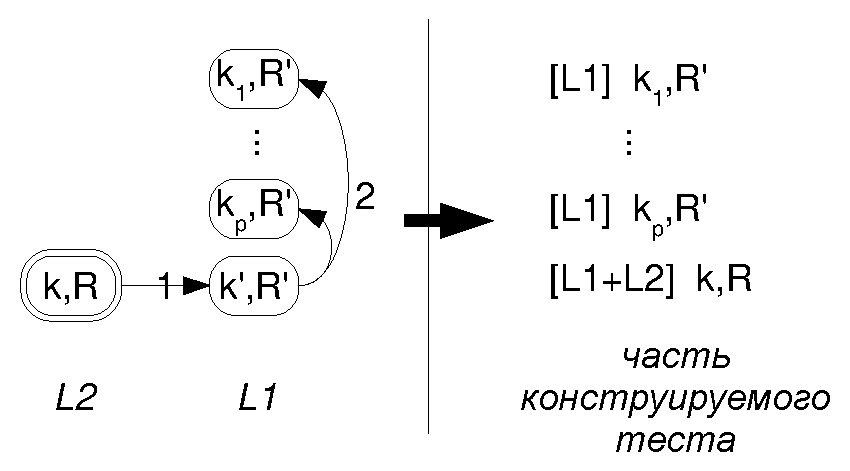
\includegraphics[width=0.6\textwidth]{2.theor/L1L2}
\caption{Конструирование обращения в кэш-память второго уровня вместе с
обращениями в кэш-память первого уровня}\label{fig:L1L2}
\end{figure}

Итак, по ключу и региону для кэш-памяти первого уровня
инструкция составляется по только что приведенной схеме. С одним лишь
уточнением, что адрес в этой инструкции должен быть таким, что при обращении по нему кэш-память
второго уровня не задействована. Теперь разберемся с последовательностью ключей
и регионов для кэш-памяти второго уровня. Рисунок~\ref{fig:L1L2} схематически
показывает, какие дополнительные инструкции надо построить для произвольного
обращения по ключу $k$ в регион $R$ кэш-памяти второго уровня. А именно, ключу
$k$ в регионе $R$ соответствует некоторый адрес, этому же адресу соответствуют и
некоторый ключ $k'$ в регионе $R'$ кэш-памяти первого уровня (стрелка с цифрой
1). Но надо еще обеспечить отсутствие этого ключа, иначе обращения в кэш-память
второго уровня не будет. Для этого надо сгенерировать небольшую
последовательность произвольных различных и не равных $k'$ ключей $k_1, k_2,
\dots, k_p$ и обратиться по ним в регион $R'$ кэш-памяти первого уровня без
затрагивания кэш-памяти второго уровня (значение числа $p$ зависит от стратегии
вытеснения).

%Рассмотрим один часто встречающийся случай кэширующих буферов,
%инициализация которого может вызывать трудности. Речь идет о
%кэш-памяти второго уровня. Зачастую кэш-память второго уровня не
%может быть инициализирована отдельно от остальных подсистем
%микропроцессора, обычно оно связано с изменением кэш-памяти первого
%уровня. Это создает дополнительные сложности при формулировании
%ограничений методом зеркальной генерации, поскольку инициализирующая
%последовательность должна подготавливать сразу два кэширующих буфера
%одновременно -- кэш-память первого уровня и кэш-память второго
%уровня. Кроме того, зачастую кэш-память второго уровня является
%совместной для хранения в ней данных и инструкций. Поэтому на
%инициализацию кэш-памяти второго уровня влияют и сами
%инициализирующие инструкции, и даже адрес расположения тестовой
%программы в памяти (от него зависит виртуальный адрес инструкций, а
%значит теги и индексы при обращении к кэш-памяти инструкций).
%
%Если принять дополнительное требование (и оно даст решение), что в
%кэш-памяти второго уровня наборы, используемые для доступа к
%инструкциям, не пересекаются с наборами, используемыми для доступа к
%данным, то генерируемые ограничения упрощаются (кэширование
%инструкций можно вообще не учитывать). С точки зрения зеркальной
%генерации это означает, что надо сформулировать требования на
%инициализирующую последовательность. Напомню, что одним из ключевых
%требований является произвольность начального состояния
%(содержимого) кэш-памяти.
%
%Предположим, что обращение к кэш-памяти второго уровня
%осуществляется при кэш-промахе в кэш-памяти первого уровня и
%кэш-память не является virtually indexed virtually
%tagged~\cite{HennessyPatterson3rd}. Для составления ограничений с
%использованием функций полезности необходимо знать, которые
%инструкции среди инициализирующей последовательности действительно
%обращаются в кэш-память второго уровня (иными словами, в каких
%инструкциях среди инициализирующей последовательности происходит
%кэш-промах при обращении к кэш-памяти первого уровня). Возможным
%решением было бы перебирать всевозможные распределения тестовых
%ситуаций в кэш-памяти первого уровня на элементах инициализирующей
%последовательности (с предварительной подготовкой этих тестовых
%ситуаций). Однако следующая лемма~\ref{special_initialization_L2}
%показывает, что для любого такого произвольного распределения
%тестовых ситуаций в кэш-памяти первого уровня существует решение со
%специальным распределением тестовых ситуаций. Это позволяет
%перебирать только такие специальные распределения тестовых ситуаций
%в кэш-памяти первого уровня. При этом вычислительная сложность
%процедуры поиска инициализирующей последовательности, дающей
%решение, изменяется от экспоненциальной от длины тестового шаблона к
%полиномиальной, что показывает лемма~\ref{max_k_h} (ее доказательство
%приведено в приложении~\ref{proofs}):
%\begin{lemma}[Верхняя оценка длины специальной инициализирующей
%последовательности для стратегии вытеснения \LRU]\label{max_k_h}\MaxUpperBoundLRU
%\end{lemma}
%\begin{sld}
%$$m = O(n)$$ где $m$ --- длина специальной инициализирующей
%последовательности, $n$ -- количество инструкций тестового шаблона.
%\end{sld}
%
%Для получения инициализирующей программы минимальной длины, можно
%применять сначала двоичный поиск суммы $k+h$ с применением
%дальнейшего поиска допустимых значений $k$ и $h$. 

\section*{Задачи}

% !Mode:: "TeX:UTF-8"

\zhead{Посчитать значения функций}

\z Для следующей алгебраической спецификации посчитать значения указанных выражений:
\begin{lstlisting}
scheme Sets = class
  type Set, Elem
  value
        empty: Unit -> Set,
        add: Elem >< Set-> Set,
        delete: Elem >< Set -> Set,
        inset: Elem >< Set -> Set
  axiom
    forall s: Set, x, y: Elem :-
        add(x, add(x, s)) is add(x, s),
        delete(x, empty() ) is delete(x, empty()),
        delete(x, add(x, s)) is delete(x, s),
        delete(x, add(y, s)) is add(y, delete(x,s)),
        ~inset(x, empty() ),
        inset(x, add(y, s)) is (x = y \/ inset(x,s)),
        inset(x, delete(y,s)) is x ~= y /\ inset(x,s)
end
\end{lstlisting}
\begin{itemize}
  \item inset(1, add(1, empty()));
  \item inset(1, delete(1, empty()));
  \item inset(1, delete(1, add(1, empty())));
  \item delete(1, add(1, empty()));
  \item delete(1, add(2, empty()));
  \item delete(1, add(1, add(1, empty())));
  \item delete(1, add(2, add(1, empty())));
  \item add(2, delete(1, add(2, add(1, empty()))));
  \item inset(3, add(2, delete(1, add(2, add(1, empty())))));
  \item inset(3, add(2, delete(3, add(2, add(1, empty())))));
  \item inset(3, add(3, delete(1, add(2, add(1, empty())))));
  \item inset(3, add(3, delete(3, add(3, add(3, empty())))));
\end{itemize}

Решение (1):
\begin{lstlisting}
inset(1, add(1, empty())) is
   1 = 1 \/ inset(1, empty()) is true
\end{lstlisting}

Решение (3):
\begin{lstlisting}
inset(1, delete(1, add(1, empty()))) is
    1 ~= 1 /\ inset(1, add(1, empty())) is false
\end{lstlisting}

Решение (4):
\begin{lstlisting}
delete(1, add(1, empty())) is delete(1, empty())
\end{lstlisting}
В данном случае произвести другие упрощения невозможно.

Обратите внимание, что
\begin{enumerate}
  \item аксиома delete(x, empty() ) is delete(x, empty()) бесполезная, потому что является тождественной истиной; ее можно безболезненно исключить из спецификации;
  \item легко выписать набор аксиом, с которым крайне тяжело работать, из них тяжело извлечь полезный смысл (тяжело ответить на нужные вопросы) --- они сводятся не к произведению полезных выводов (в т.ч. вычислений), а бездумным переписываниям.
\end{enumerate}



% !Mode:: "TeX:UTF-8"

\zhead{Ошибки в спецификациях}

\z Специфицируется АТД <<множество>> с операциями добавления и удаления элементов. Правильна ли следующая спецификация?
\begin{lstlisting}
scheme Sets = class
  type Set, Elem
  value
        empty: Unit -> Set,
        add: Elem >< Set-> Set,
        delete: Elem >< Set -> Set
  axiom
    forall s: Set, x, y: Elem :-
        add(x, add(x, s)) is add(x, s),
        delete(x, empty() ) is empty(),
        delete(x, add(x, s)) is s,
        delete(x, add(y, s)) is add(y, delete(x,s))
                pre x ~= y
end
\end{lstlisting}

\textbf{Решение:}

не соответствует (delete может оставить во множестве элемент во множестве, не удалив его, если он добавлялся несколько раз): введем функцию
\begin{lstlisting}
inset : Elem >< Set -> Bool
\end{lstlisting}
Она истинна тогда и только тогда, когда элемент есть во множестве.
\begin{lstlisting}
delete(1, add(1, add(1, empty))) is add(1, empty)
\end{lstlisting} по третьей аксиоме, но тогда
\begin{lstlisting}
inset(1, delete(1, add(1, add(1, empty)))) is
    inset(1, add(1, empty)) is true
\end{lstlisting}
а должен быть \textbf{false}, т.к. единицу должны были удалить.

Обратите внимание, что:
\begin{enumerate}
  \item методом исследования алгебраических спецификаций является исследование значений термов;
  \item чтобы получать следствия, не обязательно <<уменьшать>> терм --- может потребоваться <<навесить>> на него другие операции.
\end{enumerate}

Ответьте на вопросы:
\begin{enumerate}
  \item является ли спецификация полной?
  \item описывает ли она какие-нибудь операции полностью?
  \item является ли спецификация непротиворечивой?
\end{enumerate}

\z Специфицируется АТД <<множество>> с операциями добавления и удаления элементов. Правильна ли следующая спецификация? Полна ли? Согласована ли?
\begin{lstlisting}
scheme Sets = class
  type Set, Elem
  value
        empty: Unit -> Set,
        add: Elem >< Set-> Set,
        delete: Elem >< Set -> Set
  axiom
    forall s: Set, x, y: Elem :-
        add(x, add(x, s)) is add(x, s),
        delete(x, empty() ) is empty(),
        delete(x, add(x, s)) is delete(x, s),
        delete(x, add(y, s)) is add(y, delete(x,s))
                pre x ~= y
end
\end{lstlisting}

\z Специфицируется АТД <<множество>> с операциями добавления и удаления элементов. Правильна ли следующая спецификация? Полна ли? Согласована ли?
\begin{lstlisting}
scheme Sets = class
  type Set, Elem
  value
        empty: Unit -> Set,
        add: Elem >< Set-> Set,
        delete: Elem >< Set -> Set
  axiom
    forall s: Set, x, y: Elem :-
        add(x, add(x, s)) is add(x, s),
        delete(x, empty() ) is delete(x, empty()),
        delete(x, add(x, s)) is delete(x, s),
        delete(x, add(y, s)) is add(y, delete(x,s))
end
\end{lstlisting}

\z Специфицируется АТД <<очередь>> с операциями добавления и удаления элементов. Правильна ли следующая спецификация? Полна ли? Согласована ли?
\begin{lstlisting}
scheme Queue = class
  type Q, Elem
  value
        empty: Unit -> Q,
        add: Elem >< Q-> Q,
        delete: Elem >< Q -> Q
  axiom
    forall s: Q, x, y: Elem :-
        add(x, add(x, s)) is add(x, s),
        delete(x, empty() ) is empty(),
        delete(x, add(x, s)) is s,
        delete(x, add(y, s)) is add(y, delete(x,s))
                pre x ~= y
end
\end{lstlisting}

\z Специфицируется АТД <<стек>> с операциями добавления и удаления элементов. Правильна ли следующая спецификация? Полна ли? Согласована ли?
\begin{lstlisting}
scheme List = class
  type L, Elem
  value
        empty: Unit -> L,
        add: Elem >< L -> L,
        delete: Elem >< L -> L
  axiom
    forall s: L, x, y: Elem :-
        add(x, add(x, s)) is add(x, s),
        delete(x, empty() ) is empty(),
        delete(x, add(x, s)) is s,
        delete(x, add(y, s)) is add(y, delete(x,s))
                pre x ~= y
end
\end{lstlisting}


% !Mode:: "TeX:UTF-8"

\zhead{Неформальные интерпретации}

\z Для данной алгебраической спецификации дать неформальную интерпретацию ее типов (терминов) и операций; старайтесь увидеть случаи, в которых поведение функций не определяется в спецификации:
\begin{lstlisting}[escapechar={|}]
type E, S
value capacity: Nat,
    empty: Unit -~-> S,
    |is\_empty|: S -> Bool,
    push: S >< E -~-> S,
    pop: S -~-> S >< E,
    top: S -> Nat,
    elem: S >< Nat -~-> E,
    f: S >< E -> S f(s,e) is s,
    sc: S >< E -> S sc(s,e) is e
axiom forall s: S, e: E, i: Nat :-
  top( empty() ) is 0,
  top( push(s, e) ) is top(s) + 1
            pre top(s) < capacity ,
  top( pop(s, e) ) is top(s) - 1
            pre ~|is\_empty|(s) ,
  elem( push(s, e), top(s) + 1 ) is e
            pre top(s) < capacity ,
  elem( push(s,e), i ) is elem(s, i)
        pre i ~= top(s) + 1 /\ top(s) < capacity,
  elem( f(pop(s)), i ) is elem(s, i)
            pre i ~= top(s),
  elem( s, top(s) ) is sc(pop(s))
            pre ~|is\_empty|(s),
  |is\_empty|( empty() ),
  ~|is\_empty|( push(s,e) ),
  capacity > 0
\end{lstlisting}

Решение:
\begin{itemize}
  \item S --- структура конечного размера (capacity --- максимальный размер);
  \item empty возвращает пустую структуру;
  \item is\_empty проверяет, пуста ли структура;
  \item push помещает элемент в структуру, если после этого размер не переполнится;
  \item pop удаляет из структуры последний добавленный элемент и возвращает его вместе с измененной структурой, если структура не пустая;
  \item top вычисляет количество элементов (размер структуры);
  \item elem возвращает элемент, хранящийся в структуре по данному индексу, если значение индекса не выходит за допустимые рамки.
\end{itemize}

\z Для данной алгебраической спецификации дать неформальную интерпретацию ее типов (терминов) и операций; старайтесь увидеть случаи, в которых поведение функций не определяется в спецификации:
\begin{lstlisting}
type Owner, Auto, Warrant
value
    empty: DB,
    add: Owner >< DB -~-> DB,
    known: Owner >< DB -> Bool,
    known: Auto >< DB -> Bool,
    known: Warrant >< DB -> Bool,
    add: Owner >< Auto >< DB -~-> DB,
    add: Auto >< Warrant >< DB -~-> DB,
    get_owner: Auto >< DB -~-> Owner
axiom forall o1, o2 : Owner,
    a, a2 : Auto, db : DB, w, w2 : Warrant :-
    ~ known(o1, empty),
    known(o1, add(o2, db)) is o1 = o2 \/ known(o1, db)
            pre ~known(o2, db),
    known(o1, add(o2,a,db)) is known(o1,db)
            pre known(o2,db) /\ ~known(a,db),
    known(o1, add(a,w,db)) is known(o1,db)
            pre known(a,db) /\ ~known(w,db),

    ~ known(a, empty),
    known(a, add(o1,db)) is known(a,db)
        pre ~known(o1,db),
    known(a, add(o2,a2,db)) is a = a2 \/ known(a,db)
        pre known(o2,db) /\ ~known(a2,db),
    known(a, add(a2,w,db)) is known(a,db)
        pre known(a2,db) /\ ~known(w,db),

    ~known(w, empty),
    known(w, add(o, db)) is known(w, db)
        pre ~known(o, db),
    known(w, add(a,w2, db)) is w = w2 \/ known(w,db)
        pre known(a,db) /\ ~known(w2,db),
    known(w, add(o, a, db)) is known(w,db)
        pre known(o, db) /\ ~known(a,db),

    get_owner(a, add(o,db)) is get_owner(a, db)
        pre ~known(o, db) /\ known(a, db),
    get_owner(a, add(o, a2, db)) is if a = a2 then o
        else get_owner(a, db) end
        pre known(o,db) /\ ~known(a2, db) /\
            (a = a2 \/ known(a,db)),
    get_owner(a, add(a2,w,db)) is get_owner(a,db)
        pre known(a2,db) /\ ~known(w,db) /\
            known(a,db)
\end{lstlisting}

\z Для данной алгебраической спецификации дать неформальную интерпретацию ее типов (терминов) и операций; старайтесь увидеть случаи, в которых поведение функций не определяется в спецификации:
\begin{lstlisting}
type GTree, Person
value
    empty: Person -> GTree,
    add_child: Person >< Person >< GTree -~-> GTree,
    add_parent: Person >< Person >< GTree -~-> GTree,
    known: Person >< GTree -> Bool,
    get_childs: Person >< GTree -~-> Person-set
axiom forall p,p1,p2: Person, g: GTree :-
    known(p, empty(p1)) is p = p1,
    known(p, add_child(p1, p2, g)) is p = p2 \/ known(p,g)
        pre ~known(p2, g) /\ known(p1,g),
    known(p, add_parent(p1,p2,g)) is p = p2 \/ known(p,g)
        pre ~known(p2,g) /\ known(p1,g),

    get_childs(p, empty(p)) is {},
    get_childs(p, add_child(p1, p2,g)) is
      (if p = p1 then {p2} else {} end) union get_childs(p,g)
      pre known(p1,g) /\ ~known(p2,g) /\ known(p,g),
    get_childs(p, add_parent(p1,p2,g)) is get_childs(p,g)
      pre known(p1,g) /\ ~known(p2,g) /\ known(p,g)
\end{lstlisting}

\z Для данной алгебраической спецификации дать неформальную интерпретацию ее типов (терминов) и операций; старайтесь увидеть случаи, в которых поведение функций не определяется в спецификации:
\begin{lstlisting}
type RwS, Station, Train, TrainNumber,
    Time = Nat, Platform
value
    station: Station,
    platforms: Platform-set,
    getStart: Train -> Station,
    getEnd: Train -> Station,
    getNumber: Train -> TrainNumber,
    getStay: Train -~-> Time >< Time,
    empty: RwS,
    add_train: Train >< Platform >< RwS -~-> RwS,
    free: Platform >< Time >< Time >< RwS -~-> Bool,
    trains_tos: Station >< RwS -~-> Train-set
axiom forall t1,t2 : Time, t, tr1, tr2 : Train,
                    r : RwS, s: Station :-
    free(p, t1, t2, empty) pre p isin platforms,
    free(p, t1, t2, add_train(t,p2,r)) is
        if p ~= p2 then free(p, t1, t2,r)
        else let (s1,s2) = getStay(t) in
            t2 < s1 \/ s2 < t1 end end ),
        pre {p,p2} <<= platforms /\ t1 < t2,

    trains_tos(s, empty) is {},
    trains_tos(s, add_train(t,p,r)) is
        (if s = getEnd(t) then {t} else {} end)
            union trains_tos(s,r)
            pre p isin platforms /\
            free(p, getStart(t), getEnd(t), r),

    let (s1,s2) = getStay(t) in s1 <  s2 end,
    (getNumber(tr1) = getNumber(tr2)) is tr1 = tr2,
    platforms ~= {}
\end{lstlisting}



% !Mode:: "TeX:UTF-8"
\zhead{<<Эффект>> операций}
%% приходится добавлять обсерверы, чтобы полностью описать эффект функции

\z В~\cite{tanenbaum_os} описаны операции с файлами, среди них описана операция Create следующим образом: <<\textsf{Create} (создание). Файл создается без данных. Этот системный вызов объявляет о появлении нового файла и позволяет установить некоторые его атрибуты.>> Напишите алгебраическую спецификацию файловой подсистемы с этой операцией. Естественно, вам понадобится сигнатура этой операции. Вот она:  \texttt{int creat(char *path, int mode)}, параметр \texttt{path} содержит полное или относительное имя файла, параметр \texttt{mode} устанавливает атрибуты прав доступа различных категорий пользователей к новому файлу при его создании (если файл уже существовал, то новый не создается), операция возвращает значение файлового дескриптора для открытого файла при нормальном завершении и значение -1 при возникновении ошибки.

Решение:
\begin{lstlisting}
scheme FS = class
  type Path, Mode, FID, FS
  value
        creat : FS >< Path >< Mode -~-> FS >< FID,
        size: FS >< FID -~-> Nat,
        known: FS >< Path -> Bool,
        access: FS >< FID -~-> Mode,
        first: FS >< FID -> FS  first(a,b) is a
  axiom forall path: Path, mode: Mode, fs: FS :-
        size(creat( path, mode, fs )) is 0,
        known(first(creat( path, mode, fs )), path),
        access(creat( path, mode, fs)) is mode
end
\end{lstlisting}
Обратите внимание, что
\begin{enumerate}
  \item для описания эффекта функции \texttt{creat} были введены дополнительные операции-обсерверы;
  \item аксиомы напрямую выражают текст, описывающий операцию \texttt{creat} --- аксиомы формализуют \emph{требования} на эту операцию.
\end{enumerate}
Ответьте на следующие вопросы:
\begin{enumerate}
  \item эта спецификация неполная, почему? является ли она противоречивой? как, добавив 1 аксиому, полностью описать операцию known?
  \item имеют ли смысл сами по себе введенные дополнительные операции или они выполняют лишь вспомогательную для описания \texttt{creat} функцию?
  \item допустим, мы догадываемся, что Path = \textbf{Text}, а Mode = \textbf{Nat}; дополненная этим знанием спецификация, останется ли алгебраической ? станет ли полной ? останется ли непротиворечивой ? будет ли она соответствовать исходной постановке задачи ? не станет ли она допускать того, что не должно бы по условию ?
\end{enumerate}

\z В~\cite{tanenbaum_os} описаны операции с файлами, среди них описана операция Delete следующим образом: <<\textsf{Delete} (удаление). Когда файл уже более не нужен, его удаляют, чтобы освободить пространство на диске. Этот системный вызов присутствует в каждой операционной системе.>> Напишите алгебраическую спецификацию файловой подсистемы с этой операцией. Естественно, вам понадобится сигнатура этой операции. Вот она:  \texttt{void delete(const char *path)}, параметр \texttt{path} содержит абсолютный или относительный путь к файлу.

\z В~\cite{tanenbaum_os} описаны операции с файлами, среди них описана операция Open следующим образом: <<\textsf{Open} (открытие). Прежде чем использовать файл, процесс должен его открыть. Системный вызов open позволяет системе прочитать в оперативную память атрибуты файла и список дисковых адресов для быстрого доступа к содержимому файла при последующих вызовах.>> Напишите алгебраическую спецификацию файловой подсистемы с этой операцией. Естественно, вам понадобится сигнатура этой операции. Вот она:  \texttt{fid open(const char *path)}, параметр \texttt{path} содержит абсолютный или относительный путь к файлу.

\z В~\cite{tanenbaum_os} упомянут системный вызов mmap: <<Системный вызов mmap принимает на входе два параметра: имя фала и виртуальный адрес памяти, по которому операционная система отображает указанный файл. Для реализации отображения файлов на память изменяются системные внутренние таблицы.При обращении к памяти по адресу от 512 до 576К происходит прерывание из-за отсутствия страницы, обработчик которого предоставляет считанную в память страницу 0 файла.Если потом эта страница удаляется из памяти алгоритмом замены страниц, она записывается в соответствующее место файла.>>

%% понять, как описывать недопустимое поведение

%\zhead{Спецификация отношений <<многие-ко-многим>>}
%
%Алгебраические спецификации позволяют описать многие компоненты, осуществляющие отношение <<многие-ко-многим>>, совершенно не задумываясь о том, каким образом это отношение выразить чем-нибудь более известным (например, вспомните, сколько есть различных способов представления этого отношения для реляционной модели данных!)
%
%\z Специфицируйте компонент, отвечающий за хранение и модификацию данных о студентах Университета и спецкурсах. А именно, есть студенты, они добавляются в базу внутри этого компонента. Есть спецкурсы, которые также добавляются. Как-то студенты записываются на спецкурсы. Компонент позволяет

\zhead{Термы, конфлюэнтность}

\z Приведите несколько различных примеров типов и функций, удовлетворяющих спецификации:
\begin{lstlisting}
type E, S
value empty: S,
      add: S >< E -> S
axiom all e: E :- empty ~= add(empty,e)
\end{lstlisting}

\z Приведите несколько различных примеров типов и функций, удовлетворяющих спецификации:
\begin{lstlisting}
type E, S
value empty: S,
      add: S >< E -> S
axiom all e: E :- empty = add(empty,e)
\end{lstlisting}

\z Приведите несколько различных примеров типов и функций, удовлетворяющих спецификации:
\begin{lstlisting}
type E, S
value empty: S,
      add: S >< E -> S
axiom all e: E :- empty ~= add(empty,e),
all e: E :- empty = add(add(empty,e),e),
\end{lstlisting}

\z Приведите несколько различных примеров типов и функций, удовлетворяющих спецификации:
\begin{lstlisting}
type E, S
value empty: S,
      add: S >< E -> S
axiom all e: E :- empty ~= add(empty,e),
all e1,e2: E :- empty = add(add(empty,e1),e2),
\end{lstlisting}

\z Приведите несколько различных примеров типов и функций, удовлетворяющих спецификации:
\begin{lstlisting}
type E, S
value empty: S,
      add: S >< E -> S
axiom all e: E :- empty ~= add(empty,e),
all e1,e2: E :- empty ~= add(add(empty,e1),e2),
\end{lstlisting}

\z Приведите несколько различных примеров типов и функций, удовлетворяющих спецификации:
\begin{lstlisting}
type E, S
value empty: S,
      add: S >< E -> S
axiom all e1,e2: E :- add(empty,e1) = add(empty,e2)
\end{lstlisting}

\z Приведите несколько различных примеров типов и функций, удовлетворяющих спецификации:
\begin{lstlisting}
type E, S
value empty: S,
      add: S >< E -> S
axiom all e1,e2: E :- add(empty,e1) ~= add(empty,e2) pre e1 ~= e2,
all e1,e2: E :- add(empty,e1) = add(add(empty,e2),e1)
\end{lstlisting}




\section{Полнота и непротиворечивость алгебраических спецификаций}

% !Mode:: "TeX:UTF-8"
\head{Непротиворечивые алгебраические модели}

Алгебраическая модель непротиворечива, если из нее, как теории, нельзя вывести тождественную ложь.

При исследовании на непротиворечивость не стоит забывать утверждений об операциях и типах, не выраженных явно. Например, для операции f: T1 -> T2, определенной тотальным образом, справедливо, что all x, y: T1 :- f(x) $\Not$= f(y) => x $\Not$= y. Другой случай --- ограничения на типы входных и выходных параметров функции из сигнатуры (например, если тип Nat, то соответтсвующее значение должно быть всегда больше или равно нулю).

\head{Полные алгебраические модели}

В~\cite{mayer} написано: <<Не существует формального определения интуитивно ясного понятия <<полноты>> спецификации абстрактного типа данных. Строго определяемое понятие достаточной полноты как правило обеспечивает удовлетворительный ответ. ... Вопрос о полноте: <<Как узнать, что уже специфицировано достаточно свойств и можно остановиться?>> ... Для математика некоторая теория является полной, если ее аксиомы и правила вывода являются достаточно мощными, чтобы доказать истинность или ложность любой формулы, выразимой в языке данной теории. ... Здесь <<язык теории>> --- это множество правильно построенных выражений, т.е. тех выражений, которые можно построить, используя функции АТД, применяемые к аргументам соответствующих типов.

Спецификация АТД T является \emph{достаточно полной} тогда и только тогда, когда аксиомы ее теории позволяют для каждого выражения expr \textbf{без свободных переменных типа T} решить следующие задачи:

\begin{itemize}
\item[(S1)] Определить, является ли expr корректным (синтаксически и не нарушено не одно предусловие);
\item[(S2)] Если expr обсерверного вида и в пункте S1 установлена его корректность, то представить значение expr в виде, не включающем никаких значений типа T.
\end{itemize}

\head{Метод построения достаточно полных алгебраических спецификаций}

\begin{enumerate}
\item составить список требований на компонент (<<features>>);
\item выделить целевой и нецелевые типы, операции-генераторы, операции-обсерверы: операций должно быть достаточно для спецификации всех требований;
\item составить все аксиомы вида <<обсервер(генератор)>> для всех корректных пар обсерверов и генераторов, не забыв про предусловия;
\item проверить, все ли требования специфицированы; если не все, ввести дополнительные операции-обсерверы или аксиомы над цепочками генераторов и повторить предыдущий шаг.
\end{enumerate}

Написание аксиомы для терма <<обсервер(генератор)>> --- это по сути задание вопроса о поведении специфицируемого компонента (<<как он себя поведет, если сделать сначала это, а потом спросить про это? всегда ли он поведет себя одинаковым образом?>>) и формализация ответа на этот вопрос.

Следует помнить следующий <<психолоческий эффект>>: мы хотим в спецификации выразить одно, а выражаем лишь его часть (это уже не <<однозначная>> спецификация, а <<недоопределенная>>). Выделив обсерверы (т.е. по сути атрибуты состояния), и описав аксиомы, надо проверить, точно ли описаны требования на операцию-обсервер: не описан ли \emph{более общий} или \emph{более частный} случай, нежели требовалось (например, вместо для хранилища элементов без порядка не выражено отсутствие порядка). И не забывать, что термы в спецификациях --- это лишь символы: если автор спецификации предполагает, что эта-та функция добавляет нечто куда-то, эта проверяет вхождение, то, если должным образом не сузить различные варианты совпадений значений различных термов из генераторов, то спецификация окажется неправильной, хотя и составленной автором с полной уверенностью в своей правоте.

\head{Конструкторы}

Зачастую полезно функцию, которая задает <<структуру>> состояния. Например, список --- это всегда цепочка неких элементов. Эту цепочку можно составлять по порядку по одному элементу. Дерево --- это неким образом организованные вершины (а в вершинах полезная информация). Тогда дерево можно составлять, добавляя по одной вершине. Операции по такой <<инициализации>> целевого типа будем называть \emph{конструкторами}.

Цепочка вызовов конструкторов дает значение в целевом типе. Причем конструктором может быть только та операция, термами из которых можно получить все значения в целевом типе.

Аналогами конструкторов в языке Java и некоторых других языках программирования могут быть конструкторы объектов (\texttt{tree = new Tree(n, left, right)}).

Замечено, что если удается выделить конструктор вместо генераторов, то спецификации получаются более качественными. А именно, предлагается определять обсерверы и генераторы через конструкторы, т.е. вместо аксиом вида <<обсервер(генератор)>> нужно написать все аксиомы вида <<обсервер(конструктор)>> и <<генератор(конструктор)>>.

Если конструкторы являются тотальными функциями, удобно объединить их вместе с целевым типом в виде следующего \emph{вариантного определения}, при этом писать отдельно сигнатуры конструкторов не нужно:
\begin{lstlisting}
type E, T == empty | cons(E, T)
\end{lstlisting}

При этом удобно определить сразу же ряд обсерверов для получения данных, с которыми было сконструировано значение целевого типа (в этом примере определяется обсервер elem, возвращающий E по целевому типу T, если T был создан при помощи cons):
\begin{lstlisting}
type E, T == empty | cons(elem:E, T)
\end{lstlisting}

Будьте внимательны! В некоторых изданиях <<генераторами>> называют то, что здесь называется конструкторами, а <<трансформерами>> --- то, что здесь названо генераторами.



\section*{Задачи}

% !Mode:: "TeX:UTF-8"

\zhead{Выбор генераторов}

\z Для стека, определенного таким образом:
\begin{lstlisting}
type E, S
value empty : S,
  push: S >< E -> S,
  pop: S >< E -~-> S
\end{lstlisting}
дать достаточно полную алгебраическую спецификацию операции проверки наличия заданного элемента
\begin{lstlisting}
value include: S >< E -> Bool
\end{lstlisting}

\textbf{Решение:}
\begin{lstlisting}
type E, S
value empty : S,
  push: S >< E -> S,
  pop: S >< E -~-> S,
  include: S >< E -> Bool
axiom forall e,e1:E, s:S :-
  ~ include(e, empty),
  include(e, push(s,e1)) is e = e1 \/ include(e,s),
  include(e, pop(s)) is
     if e = top(s) then count(e,s) > 1
             else count(e,s) > 0 end  pre s ~= empty
value count: E >< S -> Nat,
      top: S -~-> E
axiom forall e,e1:E, s:S :-
   count(e, empty) is 0,
   count(e, push(s,e1)) is count(e,s) +
      if e = e1 then 1 else 0 end,
   count(e, pop(s)) is count(e,s) -
      if e = top(s) then 1 else 0 end pre s ~= empty,

   top(push(s,e1)) is e1,
   top(pop(s)) is last(s,2) pre size(s) >= 2

value last: S >< Nat -~-> E,
      size: S -> Nat
axiom forall s:S, e:E, n:Nat :-
   size(empty) is 0,
   size(push(s,e)) is size(s) + 1,
   size(pop(s)) is size(s) - 1 pre s ~= empty,

   last(push(s,e), n) is
      if n = 1 then e else last(s, n-1) end
        pre n > 0 /\ n <= size(s),
   last(pop(s), n) is last(s, n+1)
        pre s ~= empty /\ n > 0 /\ n < size(s)
\end{lstlisting}

Обратите внимание, что
\begin{enumerate}
\item при помощи выбранных для описания стека генераторов значение стека будет иметь вид, например, push(push(pop(push(empty,1)),10),1); такое выражения значения в типе стек может казаться наиболее адекватным, ведь добавление и удаление элементов --- именно те операции, при помощи которых можно изменить значение (<<состояние>>) стека; однако посмотрите, насколько увеличивается спецификация и теряется ее наглядность, если в число генераторов включена лишняя функция (pop); сравните:
\begin{lstlisting}
type E, S
value empty : S,
  push: S >< E -> S
value include: S >< E -> Bool
axiom forall e,e1:E, s:S :-
  ~ include(e, empty),
  include(e, push(s,e1)) is e = e1 \/ include(e,s),
\end{lstlisting}

\item в этом примере синтаксически разные термы из генераторов могут означать одинаковые значения типа, например, push(pop(push(empty,1)),2) и push(pop(push(empty,3)),2); в таких случаях надо быть внимательными при выписывании аксиом: помнить и понимать, сколько разных возможностей есть для рекурсивной части цепочки (речь идет о переменной <<s>> в примерах) --- например, в аксиоме с генератором, удаляющим элемент, надо в том числе предполагать, что этот элемент может появиться много раз до этого, добавляться и удаляться.
\end{enumerate}

%% минимальный набор генераторов уменьшает спецификацию (оценить количество аксиом?)

%% при нескольких генераторах надо быть аккуратными

\z Для множества, определенного таким образом:
\begin{lstlisting}
type E, S
value empty : S,
  add: S >< E -> S,
  delete: S >< E -> S
\end{lstlisting}
дать алгебраическую спецификацию операции проверки наличия заданного элемента
\begin{lstlisting}
value include: S >< E -> Bool
\end{lstlisting}

\zhead{Описание эффекта  на основе структуры терма}

Вы уже заметили, что основной принцип написания аксиомы --- понять, как вычисляется обсервер после последнего сработавшего генератора. При этом для выражения этой аксиомы используются аргументы, с которыми вызван обсервер и последний генератор. Однако не всегда просто описать эффект работы генератора на основе лишь аргументов последнего из них.

\z Дать достаточно полную алгебраическую спецификацию типа <<Ограниченная очередь>>. В эту очередь можно добавлять и удалять элементы, но только если количество хранящихся элементов не превышает заданную величину.

\textbf{Решение:}
\begin{lstlisting}
value capacity : Nat
type E, S == empty | add(E,S)
value delete: S -~-> E
axiom forall e:E, s:S :-
   delete(add(e,s)) is s
     pre size(s) < capacity

value size: S -> Nat
axiom forall e:E, s:S :-
   size(empty) is 0,
   size(add(e,s)) is size(s) + 1
       pre size(s) < capacity
\end{lstlisting}

Обратите внимание, что
\begin{enumerate}
\item пришлось добавить и описать дополнительный обсервер size;
\item существует множество способов реализации ограниченной очереди при помощи имеющихся в языках программирования средств (например, при помощи <<кольцевой очереди>>, реализованной при помощи массива и двух указателей), однако здесь предъявляется именно формализация функциональности операций, которая остается справедливой и неизменной для любой реализации <<ограниченной очереди>>;
\item данное описание не дает определения того, в каких случаях определена каждая операция в отдельности;
\item при написании аксиомы для рекурсивной части терма достаточно представлять только \emph{правильно построенные термы} --- такие термы, в которых все функции вызваны с аргументами правильных типов и в каждой функции выполнено ее предусловие; например, для аксиомы size(add(e,s)) не надо представлять, что она должна описывать и такой терм: size(add(e,add(e1,add(e2,empty)))) при capacity = 2.
\end{enumerate}

\z Дать достаточно полную алгебраическую спецификацию типа <<Исключающая очередь>>. В эту очередь элемент добавляется в том случае, если его не было, а если он там был, то он удаляется из очереди. Опишите операцию проверки наличия заданного элемента в такой очереди.


%% не всегда просто понять, полна ли спецификация
\zhead{Противоречивость алгебраических спецификаций}

Если спецификация допускает подстановку и <<вычисление>> термов увеличивающейся длины, пытаться <<вычислять>> эти термы разными способами, которые допускают аксиомы, и проверять, получаются ли одинаковые результаты в разных способах. Если получились разные, значит, найдено противоречие.

\z Противоречива ли следующая спецификация?
\begin{lstlisting}
type E, T
value empty : T,
      add: T >< E -> T,
      check: T >< E -> Bool
axiom forall e,e1: E, t: T :-
   add(add(t,e),e) is add(t,e),
   add(add(t,e),e1) is add(add(t,e1),e),
   ~check(empty, e),
   check( add(t,e1), e) is e = e1 \/ check(t,e),
\end{lstlisting}

\textbf{Решение:}
Она непротиворечива. В доказательство достаточно привести модель. Например, такую:
\begin{lstlisting}
type E, T = E-set
value empty : T = {},
      add: T >< E -> T add(t,e) is t union {e},
      check: T >< E -> Bool check(t,e) is e isin t
\end{lstlisting}

\z Противоречива ли следующая спецификация?
\begin{lstlisting}
type E, T
value empty : T,
      add: T >< E -> T,
      choose: T -~-> E
axiom forall e,e1: E, t: T :-
   add(add(t,e),e) is add(t,e),
   add(add(t,e),e1) is add(add(t,e1),e),
   choose(add(t,e)) is e
\end{lstlisting}

\textbf{Решение:}
Противоречивая. Докажем это. Поскольку верна вторая аксиома, то верно, что choose(add(add(t,e1),e2)) is choose(add(add(t,e2),e1)) для e1 $\Not$= e2. По третьей аксиоме левая часть эквивалентна e2, а правая e1, т.е. e2 is e1, что является тождественно ложным утверждением. Получено противоречие. Важным моментом здесь является то, что хотя choose может быть недетерминированной, но она эквивалентным образом должна себя вести на эквивалентных аргументах (для сравнения на равенство этот факт был бы ложным).

\z Противоречива ли следующая спецификация?
\begin{lstlisting}
type Integer = Int
value MAXINT : Integer :- MAXINT > 0
axiom all i: Integer :- abs i < MAXINT
value add: Integer >< Integer -~-> Integer
axiom forall x, y: Integer :-
   add(x, 0) is x,
   add(x, y+1) is add(x,y)+1
\end{lstlisting}

\textbf{Решение:}
Из сигнатуры add следует, что all x, y : Int :- abs x < MAXINT $\wedge$ abs y < MAXINT $\wedge$ (add определена для x и y => abs add(x,y) < MAXINT). Из первой аксиомы следует, что add(MAXINT-1, 0) определен и равен MAXINT-1. Тогда по второй аксиоме add(MAXINT-1,1) определен и равен MAXINT --- получили противоречие с тем, что аргументы функции допустимы и функция для них определена, но ее значение выходит за рамки типа. Ответ: противоречива.

\z Противоречива ли следующая спецификация?
\begin{lstlisting}
type T
value empty : T,
    put: T >< Nat -> T,
    get: T >< Nat -> Bool
axiom forall t: T, x, y, z: Nat :-
  put( put(t, x), x ) is put(t, x),
  ~get( empty, x ),
  get( put(empty, x), y ) is (x = y /\ x\2 = 0),
  get(put(put(empty,x),y),z) is (z=x /\ y\2=0) pre x\2=0,
  get( put(t, y), x ) is get(t, x) pre y ~= x,
  get( put( put(t, x), y), x ) is get( put(t,x), x ),
  ~get(put(put(t,x),x+1),x+1) pre ~get(t,x+1) /\ get(t,x)
\end{lstlisting}

\z Противоречива ли следующая спецификация?
\begin{lstlisting}
type T
value empty: T,
    put: T >< Nat -> T,
    get: T >< Nat -> Bool
axiom forall t:T, x, y, z: Nat :-
  put(put(t, x), x) is put(t, x),
  get( put (put(t, 0), x ), x) is (x > 0),
  get( put (put(t, 2*x), x ), x) is (x > 0),
  ~get( empty, x ),
  ~get( put(empty,x), y ),
  get(put(put(empty,x),y),z) is (z>0 /\ z=abs(x-y) )
\end{lstlisting}

\z Противоречива ли следующая спецификация?
\begin{lstlisting}
type T = Nat
value empty: T,
    put: T >< Nat -> T,
    get: T >< Nat -> Bool
axiom forall t: T, x, y, z: Nat :-
  put( put(t, x), y ) is put(t,x) pre y <= x,
  ~get( empty, x ),
  get( put(empty, x), y ) is (x = y),
  get(put(put(empty,x),y),z) is (z = x \/ z = y /\ y > x),
  get( put(t,x), y ) is get(t,y) pre y ~= x,
  ~get(put(t,2*y),2*y) pre get(t,y) /\
       get(t,y+1) /\~get(t,2*y),
  get( put(put(t, 0), x), x ) is get( put(t,x), x )
\end{lstlisting}

\z Противоречива ли следующая спецификация?
\begin{lstlisting}
type T
value empty: T,
    put: T >< Nat -> T,
    get: T >< Nat -> Bool
axiom forall t: T, x, y, z: Nat :-
  put( put(t, x), y ) is put(t,x) pre y <= x,
  ~get( empty, x ),
  get( put(empty, x), y ) is (x = y),
  get(put(put(empty,x),y),z) is (z = x \/ z = y /\ y > x),
  get( put(t,x), y ) is get(t,y) pre y ~= x,
  ~get( put(t, 2*y), 2*y ) pre get(t,y) /\ get(t, y+1),
  get( put(put(t, 0), x), x ) is get( put(t,x), x )
\end{lstlisting}

\z Противоречива ли следующая спецификация?
\begin{lstlisting}
type T
value empty: T,
    put: T >< Nat -> T,
    get: T >< Nat -> Bool
axiom forall t: T, x, y, z: Nat :-
  put( put(t,x), x ) is put(t,x),
  ~get( empty, x ),
  get( put(empty, x), y ) is (x = y),
  get(put(put(empty,x),y),z) is (z=x \/ z=y /\ y>2),
  get( put(t,x), y ) is get(t, y) pre y ~= x,
  get( put(t,y), y ) pre get( put(t,x), x ) /\ x <= y,
  ~get(t,x) pre get( put(t, 0), 0),
  ~get(t, x) /\ ~get(t,y) pre x ~= y /\ get(put(t,1),1)
\end{lstlisting}

\z Противоречива ли следующая спецификация?
\begin{lstlisting}
type T
value empty: T,
    put: T >< Nat -> T,
    get: T >< Nat -> Bool
axiom forall t: T, x, y, z: Nat :-
  put( put(t,x), x ) is put(t,x),
  ~get( empty, x ),
  get( put(empty, x), y ) is (x = y),
  get( put( put(empty,x), y ), z ) is (z = x \/ z = y /\ y > 0),
  get( put(t,x), y ) is get(t, y) pre y ~= x,
  get( put(t,y), y ) pre get( put(t,x), x ) /\ x <= y,
  ~get(t,x) pre get( put(t, 0), 0) /\ ~get(t,0),
  ~get(t,x) \/ ~get(t,y) pre x~=y /\ get(put(t,1),1) /\ ~get(t,1)
\end{lstlisting}

\zhead{Полнота алгебраических спецификаций}

Не забывайте, что у нас есть только система аксиом и логика, т.е. правила получения новых выражений из имеющихся. За символами имен операций не стоит никакой семантики, даже если она <<предполагалась>> автором. Наоборот, эта система аксиом должна \emph{дать} нам семантику символов, т.е. дать нам возможность сделать с этими символами некие осмысленные действия.

\z Полно ли описывает следующая спецификация тип <<Множество>> ?
\begin{lstlisting}
type E, S
value empty: S,
      add: E >< S -> S,
axiom forall e1, e2: E, s : S :-
   add(e1, add(e1, s)) is add(e1, s),
   add(e1, add(e2, s)) is add(e2, add(e1, s))
\end{lstlisting}

\textbf{Решение:}
В этой спецификации нет ни одного обсервера, поэтому вопрос о полноте для нее некорректен.

\z Полна ли следующая спецификация типа <<Очередь>> ?
\begin{lstlisting}
type E, Q
value empty: Q,
      add: E >< Q -> Q,
      size: Q -> Nat
axiom forall e: E, q : Q :-
    size(empty) is 0,
    size(add(q, e)) is size(q) + 1
\end{lstlisting}

\textbf{Решение:}
Обсервер --- size. Он определен для empty и определен для генератора add. Значит, он определен для любого терма, дающего тип Q. Значит, функция size описана полно.

\z Полна ли следующая спецификация типа <<Очередь>> ?
\begin{lstlisting}
type E, Q
value empty: Q,
      add: Q >< E -> Q,
      size: Q -> Nat
axiom forall e: E, q : Q :-
    size(empty) is 0,
    size(add(q, e)) is size(q) + 1,
    add(add(q, e), e) is add(q, e)
\end{lstlisting}

\textbf{Решение:}
Без учета последней аксиомы size(add(add(q,e),e)) is size(add(q,e)) + 1 is size(q) + 2. А теперь с последней аксиомой: size(add(add(q,e),e)) is size(add(q,e)) is size(q) + 1. Получается, что size(q) + 1 = size(q) + 2. Иными словами, из аксиом следует ложь, система аксиом противоречива. А раз так, вопрос о полноте некорректен.


\z Полна ли следующая спецификация типа <<Очередь>> ?
\begin{lstlisting}
type E, Q
value empty: Q,
      add: Q >< E -> Q,
      first: Q -~-> E,
      size: Q -> Nat
axiom forall e: E, q : Q :-
    first(add(empty, e)) is e,
    first(add(q, e)) is first(q) pre q ~= empty,
    size(empty) is 0,
    size(add(q,e)) is size(q) + 1
\end{lstlisting}

\textbf{Решение:}
Любое значение в целевом типе Q имеет один из двух видов (просто напросто, нет других функций, возвращающих Q):
\begin{itemize}
  \item empty
  \item add(add(add(...add(add(empty, e1), e2)...)
\end{itemize}

Посмотрим на first с точки зрения определения достаточной полноты. Обе аксиомы для простоты можно объединить в одну: first(add(q,e)) is if q = empty then e else first(q) end. Тогда такое выражение <<вычислить>> можно: first(add(empty,e1)) is e1 (по первой аксиоме). Посмотрим такое выражение: first(add(add(empty,e1),e2)) is if add(empty,e1) = empty then e2 else e1 end. Чтобы закончить <<вычисление>>, надо понять истинность выражения add(empty,e1) = empty. В общем случае дать ответ на этот вопрос нельзя (\emph{проблема равенства термов алгоритмически неразрешима}). Однако в данном случае ответить на этот вопрос можно.

Для этого сделаем такой хитрый ход -- \emph{<<навесим>> на эти два выражения сверху другой обсервер}: size(empty) is 0, size(add(empty,e1)) is size(empty) + 1 is 0 + 1 is 1, т.е. size(empty) $\Not$= size(add(empty,e1)). Поскольку size --- тотальная функция, то она детерминированная, т.е. all x, y : Q :- x = y => size(x) = size(y), что то же самое, что size(x) $\Not$= size(y) => x $\Not$= y. Теперь в качестве x возьмем empty, а в качестве y возьмем add(empty, e1). Получим, что add(empty, e1) $\Not$= empty. Ура, желаемое доказано! Тем самым, можно и вычислить второй терм, он равен e1. Аналогично, можно вычислить и все остальные термы.

Осталось рассмотреть единственный терм: first(empty). Если бы существовали такие q' и e', что add(q',e') равнялось empty, то было бы возможно применение аксиом. Но, как следует из первой части, такие q' и e' не существуют, значит, <<вычислить>> first(empty) на основе данных аксиом нельзя. Ответ: неполна.

\z Полна ли следующая спецификация типа <<Очередь>> ?
\begin{lstlisting}
type E, Q
value empty: Q,
      add: Q >< E -> Q,
      first: Q -~-> E,
axiom forall e: E, q : Q :-
    first(add(empty, e)) is e,
    first(add(q, e)) is first(q) pre q ~= empty,
\end{lstlisting}

\textbf{Решение:}
Рассуждая аналогично предыдущей задаче, приходим к вопросу об истинности add(empty,e1) = empty и в данной системе аксиом дать ответ на этот вопрос нельзя. Ответ: неполна.






%попробовать описать такие функции для множества как длина, вложение, вхождение элемента во множество


% !Mode:: "TeX:UTF-8"

\zhead{Алгебраические спецификации и конечные автоматы}

В каждой задаче этого типа дается алгебраическая спецификация и часть конечного автомата. Требуется ответить на вопрос, может ли конечный автомат, часть которого представлена в задаче, быть реализацией алгебраической спецификации. Положительный ответ означает наличие модели для состояний и для всех операций. В случае такого ответа требуется привести такую модель. В случае отрицательного ответа нужно этот ответ доказать.

При решении задачи следует учитывать следующие моменты:
\begin{enumerate}
\item в алгебраической спецификации ничего не сказано про структуру состояния (структуру данных состояния);
\item со структурой состояния связаны классы эквивалентности термов из генераторов (два терма эквивалентны, если при вычислении они дают одинаковые значения целевого типа);
\item в алгебраической спецификации явно не выделены некоторые важные свойства операций (обратимость, идемпотентность), но тем не менее возможен логический вывод этих свойств из аксиом;
\item не сказано, что цепочки из данных генераторов исчерпывают всё множество значений целевого типа;
\item по аксиомам вычисления значений операций-обсерверов ведутся на основе \textbf{синтаксической} структуры терма-аргумента этих обсерверов.
\end{enumerate}

При обозначении автоматов будет использоваться ряд символов. Если не сказано обратное, разным символам должны быть сопоставлены различные значения (например, $e_1$ и $e_2$ должны иметь различные значения). Состояние в конечном автомате на рисунке в задаче --- это некое конкретное состояние, а не <<обобщенное>> (например, не <<в состоянии хранится любое четное число>>, а <<в состоянии хранится число 2>>).

Для решения задачи предлагается выделять характерные особенности функциональности операций-генераторов. Если эти особенности окажутся несовместными, то ответ в задаче отрицательный. Если совместными, то по ним надо предложить и модель.

\z \begin{lstlisting}
type E, S
value empty: S,
     add: S >< E -> S,
     include: S >< E -> Bool
axiom forall s: S, e, e' : E :-
  ~include(empty, e),
  include( add(s,e'), e ) is e = e' \/ include(s,e)
\end{lstlisting}

\MediumPicture\VCDraw{\begin{VCPicture}{(0,-2)(2,3)}
% states
\State{(1,1)}{S1}
% transitions
\LoopE{S1}{add(e)}
%
\end{VCPicture}}

\textbf{Ответ:} соответствуют. Например, S --- это множество элементов типа E, add добавляет элемент к этому множеству, в состоянии на рисунке уже присутствует e.

\z \begin{lstlisting}
type E, S
value empty: S,
     add: S >< E -> S,
     include: S >< E -> Bool
axiom forall s: S, e, e' : E :-
  ~include(empty, e),
  include( add(s,e'), e ) is e = e' \/ include(s,e)
\end{lstlisting}

\MediumPicture\VCDraw{\begin{VCPicture}{(0,-2)(10,3)}
% states
\State{(1,1)}{S1} \State{(7,1)}{S2}
% transitions
\ArcL{S1}{S2}{add(e)}
\ArcL{S2}{S1}{add(e)}
%
\end{VCPicture}}

\textbf{Ответ:} соответствуют.


\z \begin{lstlisting}
type E, S
value empty: S,
     add: S >< E -> S,
     include: S >< E -> Bool
axiom forall s: S, e, e' : E :-
  ~include(empty, e),
  include( add(s,e'), e ) is e = e' \/ include(s,e)
\end{lstlisting}

\MediumPicture\VCDraw{\begin{VCPicture}{(0,-2)(20,3)}
% states
\State{(1,1)}{S1} \State{(6,1)}{S2} \State{(11,1)}{S3}
% transitions
\EdgeL{S1}{S2}{add(e)}
\EdgeL{S2}{S3}{add(e)}
%
\end{VCPicture}}

\textbf{Ответ:} соответствуют.


\z \begin{lstlisting}
type E, S
value empty: S,
     add: S >< E -> S,
     include: S >< E -> Bool
axiom forall s: S, e, e' : E :-
  ~include(empty, e),
  include( add(s,e'), e ) is e = e' \/ include(s,e)
\end{lstlisting}

\MediumPicture\VCDraw{\begin{VCPicture}{(0,-2)(20,3)}
% states
\State{(1,1)}{S1} \State{(6,1)}{S2} \State{(11,1)}{S3}
% transitions
\EdgeL{S1}{S2}{add(e)}
\EdgeL{S2}{S3}{add(e)}
\LoopE{S3}{add(e)}
%
\end{VCPicture}}

\textbf{Ответ:} соответствуют.


\z \begin{lstlisting}
type E, S
value empty: S,
     add: S >< E -> S,
     size: S -> Nat
axiom forall s: S, e : E :-
  size(empty) is 0,
  size( add(s,e) ) is size(s) + 1
\end{lstlisting}

\MediumPicture\VCDraw{\begin{VCPicture}{(0,-2)(2,3)}
% states
\State{(1,1)}{S1}
% transitions
\LoopE{S1}{add(e)}
%
\end{VCPicture}}

\textbf{Ответ:} не соответствуют. Из второй аксиомы следует, что size(add(s,e)) $\Neq$ size(s) для любых s и e. Откуда из-за тотальности size следует, что add(s,e) $\Neq$ s для любых s и e. А на картинке нашлись такие s и e, для которых это неравенство должно быть невыполнено.


\z \begin{lstlisting}
type E, S
value empty: S,
     add: S >< E -> S,
     size: S -> Nat
axiom forall s: S, e : E :-
  size(empty) is 0,
  size( add(s,e) ) is size(s) + 1
\end{lstlisting}

\MediumPicture\VCDraw{\begin{VCPicture}{(0,-2)(10,3)}
% states
\State{(1,1)}{S1} \State{(7,1)}{S2}
% transitions
\ArcL{S1}{S2}{add(e)}
\ArcL{S2}{S1}{add(e)}
%
\end{VCPicture}}

\z \begin{lstlisting}
type E, S
value empty: S,
     add: S >< E -> S,
     size: S -> Nat
axiom forall s: S, e : E :-
  size(empty) is 0,
  size( add(s,e) ) is size(s) + 1
\end{lstlisting}

\MediumPicture\VCDraw{\begin{VCPicture}{(0,-2)(10,3)}
% states
\State{(1,1)}{S1} \State{(7,1)}{S2}
% transitions
\ArcL{S1}{S2}{add(e1)}
\ArcL{S2}{S1}{add(e2)}
%
\end{VCPicture}}


\z \begin{lstlisting}
type E, S
value empty: S,
     add: S >< E -> S,
     find: S >< E -~-> E
axiom forall s: S, e, e' : E :-
  find(add(s,e'),e) is if e ~= e' then e' else find(s,e) end
\end{lstlisting}

\MediumPicture\VCDraw{\begin{VCPicture}{(0,-2)(10,3)}
% states
\State{(1,1)}{S1} \State{(7,1)}{S2}
% transitions
\ArcL{S1}{S2}{add(e1)}
\LoopE{S2}{add(e2)}
\ArcL{S2}{S1}{add(e3)}
%
\end{VCPicture}}

\z \begin{lstlisting}
type E, S
value empty: S,
     add: S >< E -> S,
     count: S >< E -> Nat
axiom forall s: S, e, e' : E :-
  count(empty,e) is 0,
  count(add(s,e'),e) is count(s,e) +
       if e = e' then 1 else 0 end
\end{lstlisting}

\MediumPicture\VCDraw{\begin{VCPicture}{(0,-2)(10,3)}
% states
\State{(1,1)}{S1} \State{(7,1)}{S2}
% transitions
\ArcL{S1}{S2}{add(e1)}
\ArcL{S2}{S1}{add(e2)}
%
\end{VCPicture}}


\z \begin{lstlisting}
type E, S
value empty: S,
     add: S >< E -> S,
     count: S >< E -> Nat
axiom forall s: S, e, e' : E :-
  count(empty,e) is 0,
  count(add(s,e'),e) is count(s,e) +
       if e = e' then 1 else 0 end
\end{lstlisting}

\MediumPicture\VCDraw{\begin{VCPicture}{(0,-2)(10,3)}
% states
\State{(1,1)}{S1} \State{(7,1)}{S2}
% transitions
\ArcL{S1}{S2}{add(e1)}
\ArcR{S1}{S2}{add(e2)}
%
\end{VCPicture}}


\z \begin{lstlisting}
type E, S
value empty: S,
     add: S >< E -> S,
     count: S >< E -> Nat
axiom forall s: S, e, e' : E :-
  count(empty,e) is 0,
  count(add(s,e'),e) is count(s,e) +
       if e = e' then 1 else 0 end
\end{lstlisting}

\MediumPicture\VCDraw{\begin{VCPicture}{(0,-2)(10,3)}
% states
\State{(1,1)}{S1} \State{(7,1)}{S2}
% transitions
\ArcL{S1}{S2}{add(e)}
\ArcL{S2}{S1}{add(e)}
%
\end{VCPicture}}


\z \begin{lstlisting}
type E, S
value empty: S,
     add: S >< E -> S,
     count: S >< E -> Nat
axiom forall s: S, e, e' : E :-
  count(empty,e) is 0,
  count(add(s,e'),e) is count(s,e) +
       if e = e' then 1 else 0 end
\end{lstlisting}

\MediumPicture\VCDraw{\begin{VCPicture}{(0,-2)(10,3)}
% states
\State{(1,1)}{S1} \State{(7,1)}{S2}
% transitions
\ArcL{S1}{S2}{add(e1)}
\ArcL{S2}{S1}{add(e2)}
%
\end{VCPicture}}


\z \begin{lstlisting}
type E, S
value empty: S,
     add: S >< E -> S,
     include: S >< E -> Bool,
     uniq: S -> S
axiom forall s:S, e,e':E :-
  ~include(empty, e),
  include(add(s,e'),e) is e=e' \/ include(s,e),
  uniq(empty) is empty,
  uniq(add(s,e)) is if include(s,e) then uniq(s)
    else add(uniq(s),e) end
\end{lstlisting}

\MediumPicture\VCDraw{\begin{VCPicture}{(0,-2)(10,3)}
% states
\State{(1,1)}{S1} \State{(6,1)}{S2} \State{(11,1)}{S3}
% transitions
\EdgeL{S1}{S2}{uniq}
\EdgeL{S2}{S3}{uniq}
%
\end{VCPicture}}

\textbf{Решение:} не соответствуют. Докажем свойство \emph{идемпотентности} операции uniq, т.е. uniq(uniq(s)) is uniq(s) для любого s, индукцией по длине терма s. Для s = empty свойство идемпотентности выполнено по третьей аксиоме. Пусть оно выполнено для некоторого s. Рассмотрим uniq(uniq(add(s,e))) для произвольного e. По последней аксиоме это выражение равно if include(s,e) then uniq(uniq(s)) else uniq(add(uniq(s),e)) end is if include(s,e) then uniq(s) else uniq(add(uniq(s),e)) end. Осталось показать, что если $\Not$ include(s,e), то uniq(add(uniq(s),e)) is add(uniq(s),e). Опять применим последнюю аксиому: uniq(add(uniq(s),e)) is if include(uniq(s),e) then uniq(uniq(s)) else add(uniq(uniq(s)),e) end is if include(uniq(s),e) then uniq(s) else add(uniq(s),e) end. Если будет показано, что include(s,e) is include(uniq(s),e), то всё доказательство будет завершено. Покажем это снова индукцией по длине терма s. Для s = empty это верно по третьей аксиоме. Пусть это свойство доказано для некоторого s. Покажем, что include(add(s,e'),e) is include(add(uniq(s),e'),e). Распишем левую часть по второй аксиоме: include(add(s,e'),e) is e=e' $~\Or~$ include(s,e). Распишем правую часть: if include(s,e') then include(uniq(s),e) else include(add(uniq(s),e'),e) end is if include(s,e') then include(s,e) else include(add(uniq(s),e'),e) end is if include(s,e') then include(s,e) else e=e` $~\Or~$ include(s,e) end is include(s,e) $~\Or~$ (e=e`) $~\And~$ $\Not$include(s,e') is (e=e') $~\Or~$ include(s,e). Обе части совпали. Тем самым свойство идемпотентности операции uniq доказано полностью.

\z \begin{lstlisting}
type E, S
value empty: S,
     add: S >< E -> S,
     include: S >< E -> Bool,
     uniq: S -> S
axiom forall s:S, e,e':E :-
  ~include(empty, e),
  include(add(s,e'),e) is e=e' \/ include(s,e),
  uniq(empty) is empty,
  uniq(add(s,e)) is if include(s,e) then uniq(s)
    else add(uniq(s),e) end
\end{lstlisting}

\MediumPicture\VCDraw{\begin{VCPicture}{(0,-2)(10,3)}
% states
\State{(1,1)}{S1} \State{(7,1)}{S2}
% transitions
\ArcL{S1}{S2}{uniq}
\ArcL{S2}{S1}{uniq}
%
\end{VCPicture}}


\z \begin{lstlisting}
type E, S
value empty: S,
     add: S >< E -> S,
     include: S >< E -> Bool,
     uniq: S -> S
axiom forall s:S, e,e':E :-
  ~include(empty, e),
  include(add(s,e'),e) is e=e' \/ include(s,e),
  uniq(empty) is empty,
  uniq(add(s,e)) is if include(s,e) then uniq(s)
    else add(uniq(s),e) end
\end{lstlisting}

\MediumPicture\VCDraw{\begin{VCPicture}{(0,-2)(10,3)}
% states
\State{(1,1)}{S1} \State{(5,1)}{S2}  \State{(9,1)}{S3}
% transitions
\EdgeL{S1}{S2}{add(e)}
\LoopS{S2}{add(e)}
\EdgeL{S2}{S3}{uniq}
%
\end{VCPicture}}


\section{Cпецификация рекурсивных типов}

%\head{Рекурсивное определение типов (деревьев)}
Алгебраические модели и АТД являются удобным способом рекурсивного задания типов и операций их обработки. Для этого представленный только что формальный метод построения достаточно полных алгебраических спецификаций прочитывается следующим способом:
\begin{enumerate}
  \item выделить и составить сигнатуры конструкторов (пустое значение | составление нового <<узла дерева>>);
  \item выделить и составить сигнатуры функций-обработчиков рекурсивного типа;
  \item описать результат обработки для каждого конструктора.
\end{enumerate}

Например, спецификация функции, вычисляющей глубину бинарного дерева, согласно этому методу получается такой:
\begin{lstlisting}
type Node, Tree == empty | mk_tree(Node, Tree, Tree)
value depth: Tree -> Nat
axiom forall n: Node, left: Tree, right: Tree :-
  depth( empty ) is 0,
  depth( mk_tree(n, left, right) ) is
          max( depth(left), depth(right) )
value max: Nat >< Nat -> Nat
   max(x,y) is if x > y then x else y end
\end{lstlisting}

Конструктор предназначена лишь для структурных целей, т.е. определение дерева в виде типа Tree из этого примера пойдет и для бинарного дерева произвольного вида, и для бинарного сбалансированного дерева, и для других бинарных деревьев. А уже менее тривиальные функции составления деревьев (например, чтобы не нарушалась сбалансированность) определяются в виде функций-обработчиков.

\section*{Задачи}
%
\zhead{}%Рекурсивные типы}
%
\z Специфицируйте операцию проверки вхождения элемента в бинарное дерево.

\textbf{Решение:}
\begin{lstlisting}
type Node, Tree == empty | add(Node, Tree, Tree)
value check: Node >< Tree -> Bool
axiom forall n, n1:Node, left, right: Tree :-
   ~check( empty ),
   check(n, add(n1,left,right) ) is (n = n1) \/
             check(n, left) \/ check(n, right)
\end{lstlisting}

\z Специфицируйте операцию вычисления высоты бинарного дерева.

\z Специфицируйте операцию проверки бинарного дерева на сбалансированность.

\z Специфицируйте операцию получения предка элемента бинарного дерева.

\z Специфицируйте добавление элемента в двоичное дерево поиска.

\z Специфицируйте удаление элемента из двоичного дерева поиска.

\z Специфицируйте добавление элемента в АВЛ-дерево. Определение операции предполагается найти самостоятельно.

\z Специфицируйте удаление элемента из АВЛ-дерева. Определение операции предполагается найти самостоятельно.

\z Специфицируйте добавление элемента в 2-3-дерево. Определение операции предполагается найти самостоятельно.

\z Специфицируйте удаление элемента из 2-3-дерева. Определение операции предполагается найти самостоятельно.

\z Специфицируйте добавление элемента в декартово дерево. Определение операции предполагается найти самостоятельно.

\z Специфицируйте удаление элемента из декартова дерева. Определение операции предполагается найти самостоятельно.

\z Специфицируйте добавление элемента в красно-чёрное дерево.  Определение операции предполагается найти самостоятельно.

\z Специфицируйте удаление элемента из красно-чёрного дерева.  Определение операции предполагается найти самостоятельно.

% специфицировать стратегии вытеснения



\chapter{Моделе-ориентированные спецификации}

Моделе-ориентированные спецификации, как и алгебраические, описывают семантику интерфейсов программных компонент. Они основываются на \emph{абстракции алгоритмов} и \emph{абстракции данных}.

Абстракция алгоритмов предполагает, что для функций задаются (\emph{специфицируются}) не алгоритмы, их реализующие, а дается определение осуществляемого функцией отображения входных данных на выходные. Для этого зачастую используется аппарат \emph{программных контрактов}.

Абстракция данных предполагает, что для состояния компонента и типов параметров функций компонента (входных и выходных) указывается не их выражение в терминах целевого языка программирования (или их эквивалентов), а смысл, семантику этих данных, исходя из логического содержания и требований на внутренние отношения составляющих частей состояния. Например, если эти части \emph{<<по логике>>} должны быть неупорядочены и без повторов, то для моделирования таких частей следует использовать \emph{множества}. Если важен порядок и возможны повторы, то \emph{списки}. Если логически выделяются отображение одних данных в другие (отображение ключа в данные), то \emph{отображения}. Отображения являются наиболее адекватным представлением данных, которые по сути представляются <<реляционным отношением>> с первичным ключом.

В тексте реализации типы (наверняка) будут иметь другое представление, адекватное языку программирования (например, если система реализуется на Си, то вместо множеств или списков будут указатели), но логически функция в реализации должна принимать те же параметры (синтаксически функции передается указатель, а на самом деле этот указатель будет обозначать множество или список) и осуществлять то же отображение входных на выходные параметры, как это указано в спецификации.

\section{Множества, списки, отображения}

\head{Множества}
Множество -- это контейнер элементов одного типа, который обладает свойствами уникальности и неупорядоченности его элементов. Множества бывают конечными и бесконечными.

Типовое выражение для конечного множества: $typeexpr\Set$. Типовое выражение для бесконечного множества: $typeexpr\Infset$. Конечное множество -- подтип бесконечного множества.

Операции над множествами:
\begin{list}{}{}
\item $= : T\Infset \DP T\Infset \Fn \Bool$ -- сравнение на равенство
\item $\neq : T\Infset \DP T\Infset \Fn \Bool$ -- сравнение на не равенство
\item $\Union: T\Infset \DP T\Infset \Fn T\Infset$ -- объединение пары множеств
\item $\Union: T\Infset\Infset \Fn T\Infset$ -- объединение множества множеств
\item $\Inter: T\Infset \DP T\Infset \Fn T\Infset$ -- пересечение пары множеств
\item $\Inter: T\Infset\Infset \Fn T\Infset$ -- пересечение множества множеств
\item $\Minus: T\Infset \DP T\Infset \Fn T\Infset$ -- вычитание множеств
\item $\Isin: T \DP T\Infset \Fn \Bool$ -- проверка на принадлежность
\item $\NotIsin: T \DP T\Infset \Fn \Bool$ -- проверка на непринадлежность
\item $\SetL: T\Infset \DP T\Infset \Fn \Bool$ -- проверка вложения
\item $\SetG: T\Infset \DP T\Infset \Fn \Bool$ -- проверка вложения
\item $\SetLE: T\Infset \DP T\Infset \Fn \Bool$ -- проверка вложения
\item $\SetGE: T\Infset \DP T\Infset \Fn \Bool$ -- проверка вложения
\item $\Card: T\Infset \NonDetermFn \Nat$ -- количество элементов
($\Chaos$ для бесконечных множеств)
\end{list}

Обратите внимание на отсутствие операции выбора произвольного элемента из множества!

Только операция \textbf{card} дает целое число от множеств, т.е. любое целочисленное выражение над множествами будет мощностью некоторого множества.

Конструкторы множеств:
\begin{list}{}{}
\item (\emph{пустое множество}) \{\}
\item (\emph{перечисление}) \{0, 1, 2\} - множество, состоящее из трех целых чисел (не
натуральных!) - нуля, единицы и двойки.
\item (\emph{диапазон}) \{0..2\} -  то же, что и \{0, 1, 2\};
\{0..0\} $\Iden$ \{0\}, \{1..0\} $\Iden$ \{\}
\item (\emph{<<сокращенная запись>>}) $\{ expr\_with\_var | var : typeexpr
\SuchAs boolexpr\}$ (например, $\{2 \star n | n : \Nat \SuchAs n < 3
\}$, что эквивалентно \{0, 2, 4\})
\end{list}

\head{Списки}
Список -- это контейнер элементов одного типа, который обладает свойствами упорядоченности элементов. Для задания списка надо указать не только сами элементы, но и их порядок. Списки бывают конечными и бесконечными.

Типовое выражение для конечного списка: $typeexpr\List$. Типовое выражение для бесконечного списка: $typeexpr\Inflist$. Конечный список -- подтип бесконечного списка.

Операции:
\begin{list}{}{}
\item $=: T\Inflist \DP T\Inflist \Fn \Bool$ -- проверка на равенство
\item $\neq: T\Inflist \DP T\Inflist \Fn \Bool$ -- проверка на не равенство
\item $(.) : T\Inflist \DP \Int \NonDetermFn T$ -- взятие элемента по
индексу ($\Chaos$ для индекса, отсутствующего в списке, индексы
нумеруются \textbf{с единицы})
\item $\Concat: T\List \DP T\Inflist \Fn T\Inflist$ -- конкатенация списков
\item $\Hd: T\Inflist \NonDetermFn T$ -- головной элемент списка ($\Chaos$ для пустого списка)
\item $\Tl: T\Inflist \NonDetermFn T\Inflist$ -- хвостовая часть списка ($\Chaos$ для пустого списка)
\item $\Len: T\Inflist \NonDetermFn \Nat$ -- количество элементов списка ($\Chaos$ для бесконечного списка)
\item $\Elems: T\Inflist \Fn T\Infset$ -- множество элементов списка (без повторений!)
\item $\Inds: T\Inflist \Fn \Nat\Infset$ -- множество индексов элементов списка
\end{list}

Конструкторы списков:
\begin{list}{}{}
\item (\emph{пустой список}) $\LL\LR$
\item (\emph{перечисление}) $\LL 0, 1, 2 \LR$ - список, состоящий из трех целых чисел (не натуральных!) - нуля, единицы и двойки - в порядке увеличения.
\item (\emph{диапазон}) $\LL 0..2 \LR$ -  то же, что и $\LL 0, 1, 2 \LR$; $\LL 0..0 \LR \Iden \LL 0 \LR$, $\LL 1..0 \LR \Iden \LL\LR$
\item (\emph{<<сокращенная запись>>}) $\LL expr\_with\_var | var \In listexpr \SuchAs boolexpr\LR$ (например, $\LL 2 \star n | n \In \LL 0..2 \LR \LR$, что эквивалентно $\LL 0, 2, 4 \LR$)
\end{list}


\head{Отображения}
Отображение -- это множество пар элементов, у которого первые компоненты не повторяются. Отображения бывают конечными и бесконечными, детерминированными и недетерминированными (это те, в которых первые компоненты всё же могут повторяться в разных парах).

Типовое выражение для детерминированного отображения: $$typeexpr_1 \Map typeexpr_2$$ Типовое выражение для недетерминированного отображения: $$typeexpr_1 \NonDeterMap typeexpr_2$$

Операции:
\begin{list}{}{}
\item $=: (T_1 \Map T_2) \DP (T_1 \Map T_2) \Fn \Bool$ -- сравнение отображений на равенство
\item $\neq: (T_1 \Map T_2) \DP (T_1 \Map T_2) \Fn \Bool$ -- сравнение отображений на не равенство
\item $(.): (T_1 \Map T_2) \DP T_1 \NonDetermFn T_2$ -- взятие значения по индексу ($\Chaos$, если значение по этому индексу не
определено)
\item $\Dom: (T_1 \Map T_2) \Fn T_1\Infset$ -- \emph{область определения} отображения
\item $\Rng: (T_1 \Map T_2) \Fn T_2\Infset$ -- \emph{область значения} отображения
\item $\Upd: (T_1 \Map T_2) \DP (T_1 \Map T_2) \Fn (T_1 \Map T_2)$ -- обновление отображения
\item $\Union: (T_1 \Map T_2) \DP (T_1 \Map T_2) \Fn (T_1 \NonDeterMap T_2)$ -- объединение отображений
\item $\Minus: (T_1 \Map T_2) \DP T_1\Infset \Fn (T_1 \Map T_2)$ -- уменьшение отображения
\item $/: (T_1 \Map T_2) \DP T_1\Infset \Fn (T_1 \Map T_2)$ -- проекция отображения
\item $\Superp: (T_2 \Map T_3) \DP (T_1 \Map T_2) \Fn (T_1 \Map T_2)$ -- композиция отображений
\end{list}

Конструкторы отображений:
\begin{list}{}{}
\item (\emph{пустое отображение}) []
\item (\emph{перечисление}) $[0 \mapsto 1, 1 \mapsto 2]$ -- отображение, состоящий из двух пар целых чисел (не натуральных!) - из 0 в 1 и из 1 в 2.
\item (\emph{<<сокращенная запись>>}) $[expr_1\_with\_var \mapsto expr_2\_with\_var | var : typeexpr \SuchAs boolexpr]$ (например, $[n \mapsto n+1 | n : \Nat \SuchAs n < 3]$, что эквивалентно $[0 \mapsto 1, 1 \mapsto 2, 2 \mapsto 3]$)
\end{list}


\section*{Задачи}

\zhead{Вычислить выражения с множествами}

\z $\{1, 2\} = \{3, 1\}$
\z $\{1, 2\} = \{2, 1\}$
\z $\{1, 2, 1\} = \{2, 2, 1\}$
\z $\{1, 2\}~\Union~\{3, 4\}$
\z $\{1, 2\}~\Union~\{2, 3\}$
\z $\{1, 2\}~\Inter~\{3, 4\}$
\z $\{1, 2\}~\Inter~\{2, 3\}$
\z $\{1..30\}~\Union~\{10..-10\}$
\z $\{1..30\}~\Inter~\{10..-10\}$
\z $\{1..30\}~\Union~\{x~|~ x: \Int~\SuchAs~\Abs x < 11 \}$
\z $\{1..30\}~\Inter~\{x~|~ x: \Int~\SuchAs~\Abs x < 11 \}$
\z $\{x+10 ~|~ x: \Int \} = \{x ~|~ x: \Int\}$
\z $\{5*k + 2 ~|~ k : \Int \}~\Inter~\{3*k - 1 ~|~ k : \Int\}$
\z $\{5*k + 2 ~|~ k : \Int \}~\Minus~\{3*k - 1 ~|~ k : \Int\}$
\z $\{5*k + 2 ~|~ k : \Int \} \SetL \{3*k - 1 ~|~ k : \Int\}$
\z $\{5*k + 2 ~|~ k : \Int \} \SetGE \{3*k - 1 ~|~ k : \Int\}$
\z $\Not (\{1, 2\} \SetLE \{2, 1, 1\})$
\z $\Card \{1..30\}$
\z $\Card \{5*k + 2 ~|~ k : \Int~\SuchAs~k * k \Isin \{-10..10\}\}$
\z $\Card \{5*k + 2 ~|~ k : \Int~\SuchAs~k * k \Isin \{10..-10\}\}$
\z $\Card \{k*k - 2 * k ~|~ k : \Int~\SuchAs~k * k \Isin \{-10..10\}\}$
\z $\All x: \Nat ~\SuchAs~ x \Isin \{x ~|~ x : \Int\}$
\z $\All x: \Int ~\SuchAs~ x \Isin \{x ~|~ x : \Nat\}$


\zhead{Решите уравнения}

\z $\{1\} \Union x = \{\}$
\z $\{1\} \Union x = \{1\}$
\z $\{1\} \Union x = \{1, 2\}$
\z $\{1\} \Inter x = \{\}$
\z $\{1\} \Inter x = \{1\}$
\z $\{1\} \Inter x = \{1, 2\}$
\z $\{2, 1\} \Minus x = \{1\}$
\z $\Card~x = 0$
\z $\Card~x = 1$


\zhead{Какие из следующих выражений истинные}
Считайте, что свободные переменные располагаются под квантором
всеобщности

\z $(A \cup B) \setminus C = (A \setminus C) \cup (B \setminus C)$
\z $(A \setminus B) \cap C = (A \cap C) \setminus B$
\z $(A \cup B) \setminus C \Iden (A \setminus C) \cup (B \setminus C)$
\z $A \cup \{\} = A$
\z $\{\} \cup A = A$
\z $(A \cup B) \cap C = (A \cap C) \cup (B \cap C)$
\z $\Card \Nat < \Card \Int$
\z $\Card \Nat = \Card \Int$
\z $\Card \Nat > \Card \Int$
\z $\Card \Nat \Iden \Card \Int$
\z $\Card \{n ~|~ n:\Nat\} \Iden \Card \{n ~|~ n:\Int\}$


\zhead{Записать на RSL следующие множества}

\z Пустое множество;
\z Множество чисел 1, 2, 3 (а также множество чисел от 1 до 3);
\z Множество всех чётных чисел;
\z Множество всех чётных чисел, не превышающих 10 (привести в виде перечисления и нескольких различных сокращённых формах);
\z Множество всех простых натуральных чисел;
\z Множество всех пар взаимнопростых натуральных чисел;
\z Множество всех троек, в каждой из которых есть одинаковые элементы;
\z Множество всех степеней двойки, не превышающих 100 (привести в виде перечисления и нескольких сокращённых формах);
\z Множество всех IP-адресов класса А (B, C, D, E);
\z Множество всех точек плоскости, образующих
    \begin{enumerate}
    \item Прямую -- биссектрису I и III квадрантов;
    \item Правую полуплоскость;
    \item Нижнюю полуплоскость;
    \item Единичную окружность;
    \item Единичный круг;
    \item Единичный квадрат со сторонами, параллельными осям
    координат.
    \end{enumerate}

%\zhead{Построить явную спецификацию на RSL для следующих задач}
%
%В этих задачах, если удаётся, следует привести два варианта решения: с использованием сокращённой записи множества
%и с помощью рекурсии.
%
%\z Дано множество чисел. Вернуть множество квадратов чисел данного множества.
%\z Дано множество чисел. Вернуть множество чисел, представимых суммами каких-либо двух элементов исходного множества.
%\z Дано множество точек, заданных координатами в плоской декартовой системе координат. Получить проекцию этого множества на ось \textsc{Ox}.
%\z Дано множество всех простых чисел. Для данного числа вернуть множество его простых делителей, используя множество всех простых чисел.
%\z Дано множество чисел. Дано число. Существует ли подмножество данного множества чисел, сумма элементов которого, равна данному числу.
%\z Дано множество множеств. Вернуть множество всех элементов внутренних множеств.
%\z \textit{(Задача о рюкзаке)} Дано множество предметов. Каждый предмет имеет массу (массы заданы множеством пар предмет >< масса). Есть $n$ рюкзаков. Каждый рюкзак имеет вместимость $K$ кг. Распределить все предметы по рюкзакам, не превышая вместимости каждого рюкзака.
%\z Рабочая группа компьютеров задаётся IP-адресом (4 целых числа, каждое от 0 до 255) и маской (целое число от 0 до 32). Программа по данному заданию строит множество всех возможных в ней IP-адресов.


\zhead{Вычислить выражения со списками}
\z $\LL 1 \LR = \LL 1, 1 \LR$
\z $\LL 1, 2 \LR = \LL 3, 1\LR$
\z $\LL 1, 2\LR = \LL 2, 1\LR$
\z $\LL 1, 2, 3 \LR (2)$
\z $\LL 1 \LR (0)$
\z $\LL 1 \LR (1)$
\z $\LL 1, 2\LR \Concat \LL 3, 4\LR$
\z $\LL 1, 2\LR \Concat \LL 2, 3\LR$
\z $\LL x+10~|~x~\In~\LL 1, 2 \LR \LR = \LL x~|~x~\In~\LL 1 \LR \LR$
\z $\Hd \LL 1, 2, 3 \LR$
\z $\Tl \LL 1, 2, 3 \LR$
\z $\Len \LL 1, 2, 3 \LR$
\z $\Elems \LL 1, 2, 3 \LR$
\z $\Inds \LL 1, 2, 3 \LR$
\z $\Len \LL 1..30\LR$
\z $\Let~x = \LL 1, 2, 3\LR~\In~\Elems~x~\Inter~\Inds~x~\rslEnd$
\z $\Let~x = \LL 0, 1, 2\LR~\In~\Elems~x~\Inter~\Inds~x~\rslEnd$
\z $\Let~x : \Int\Inflist~\SuchAs~(\All i_1, i_2: \Nat~\SuchAs~\Card \{i_1, i_2\} = \Card \{x(i_1), x(i_2)\})\\\In~x~\rslEnd$
\z $\Let~x : \Int\Inflist~\SuchAs~(\All i_1, i_2: \Nat~\SuchAs~\Card \{i_1, i_2\} = \Card \{x(i_1), x(i_2)\})\\\In~\Elems~x~\Inter~\Inds~x~\rslEnd$
\z $\All x : T\Inflist~\SuchAs~x(0) = \Hd x$
\z $\All x : T\Inflist~\SuchAs~x(0) ~\Iden~ \Hd x$

\zhead{Решите уравнения}
\z $\LL 1 \LR \Concat x  = \LL 1 \LR$
\z $\LL 1 \LR \Concat x  = \LL 1, 2, 3 \LR$
\z $\LL 1 \LR \Concat x  = \LL 3, 2, 1 \LR$
\z $\Tl x = \LL 1 \LR$
\z $\Hd x = 1$
\z $x \Concat \Tl x = x$
\z $\Tl x = \LL \Hd x \LR$
\z $\Elems x = \Inds x$
\z $\Elems~\Tl x = \Elems x$
\z $\Len x = \Card \Elems x$
\z $\Len x = \Card \Inds x$
\z $\Len x \Iden \Card \Inds x$


\zhead{Записать на RSL следующие выражения}

\z Пустой список;
\z Список из чисел 1, 2, 3 (попробуйте привести как можно больше различных решений);
\z Список всех простых натуральных чисел в порядке увеличения их значения;
\z Список всех пар взаимнопростых натуральных чисел в порядке увеличения их суммы;
\z Список номеров групп 5го курса факультета ВМиК МГУ в порядке увеличения номера группы;
\z Количество простых чисел от 1 до 10 (тремя различными способами).

%\zhead{Напишите явные спецификации следующих функций}
%
%\z Определить, является ли бесконечным данный список.
%\z Вычислить длину списка без использования функции $\Len$.
%\z Вычислить сумму элементов списка.
%\z Вычислить произведение элементов списка.
%\z Дан список. Построить список из элементов исходного списка, элементы которого идут в обратном порядке по отношению к исходному списку
%\z Дана строка и символ. Определить, встречается ли символ в данной строке (предложить два различных способа решения).
%\z Дана строка. Определить самый часто встречающийся в ней символ.
%\z Отсортировать данный список вещественных чисел в порядке возрастания.
%\z Построить список всех целых чисел в порядке неубывания модуля.
%\z Определить $\sup$ списка вещественных чисел (в случае конечного списка это будет и максимум).
%\z Выдать число, не встречающееся в данном списке.
%\z Дан список чисел. Построить по нему список квадратов, расположив элементы
%    \begin{enumerate}
%    \item с сохранением порядка исходного списка
%    \item в порядке убывания модуля
%    \item так, чтобы не было трёх подряд чисел, расположенных в  порядке возрастания или убывания.
%    \end{enumerate}
%\z Дано натуральное число. Построить список степеней его простых делителей, в котором на местоположение степени есть её основание (а значение, соответственно, показатель).
%\z Дан список показателей степеней (местоположение -- основание степени). Построить соответствующее натуральное число.
%\z Дан список натуральных чисел, отличных от нуля. Вернуть список, в котором на месте №$i$ находится количество раз, которое $i$ встречается в исходном списке.
%\z Дано множество чисел. Построить из него список, расположив элементы множества
%    \begin{enumerate}
%    \item в порядке убывания
%    \item в порядке убывания модуля
%    \end{enumerate}
%\z Дан список чисел. Построить из него новый список, расположив элементы исходного списка
%    \begin{enumerate}
%    \item в порядке убывания
%    \item в порядке убывания модуля
%    \end{enumerate}
%\z Дан список из чисел. Построить из него множество, использовав все элементы данного списка.
%\z Дан множество пар (ключ, объект) и список ключей. Построить соответствующий ему список объектов. Считайте, что во множество пар ключи не повторяются.
%\z Дан список чисел. Можно ли суммой некоторых его элементов получить
%    \begin{enumerate}
%    \item четное число (для списка из целых чисел)
%    \item простое число (для списка из целых чисел)
%    \item целое число (для списка из вещественных чисел)
%    \end{enumerate}


\zhead{Упростить выражения}
\z $\langle x ~|~ x~\In~\langle \Card \{a..b\} \rangle \rangle$
\z $\langle c ~|~ c~\In~\langle 'a',~'b' \rangle \rangle$
\z $\langle c ~|~ c~\In~\langle '$ " $~' \rangle \rangle$
\z $\langle c ~|~ c~\In~\langle \rangle \rangle$

\newcommand{\Masha}{\mbox{\textrm{<<Маша>>}}}
\newcommand{\Sveta}{\mbox{\textrm{<<Света>>}}}
\newcommand{\Misha}{\mbox{\textrm{<<Миша>>}}}
\newcommand{\Slava}{\mbox{\textrm{<<Слава>>}}}
\newcommand{\Anna}{\mbox{\textrm{<<Аня>>}}}
\newcommand{\Petr}{\mbox{\textrm{<<Петя>>}}}
\newcommand{\Lesha}{\mbox{\textrm{<<Леша>>}}}
\newcommand{\Victor}{\mbox{\textrm{<<Витя>>}}}

\zhead{Вычислить}

\z $\map{n \mapsto 1}{n : \Nat \SuchAs n \Isin \{1..3\} }$
\z $\map{n \mapsto n}{n : \Nat \SuchAs n \Isin \{5..5\} }$
\z $\map{n \mapsto n+1}{n : \Nat \SuchAs n \Isin \{100..90\} }$
\z $\map{n \mapsto m}{n, m : \Nat \SuchAs n \backslash m = 0 \And m > 2}$
\z $\map{n \mapsto m}{n, m : \Nat \SuchAs n \Isin \{1..3\} \And m \Isin \{1..n\}}$
\z $\map{n \mapsto (p, q)}{n, p, q : \Nat \SuchAs n \Isin \{1..100\} \And p + q = n \And p \backslash q = 0}$
\z $[1 \mapsto 2,~2 \mapsto 3,~ 3 \mapsto 1] (3)$
\z $[1 \mapsto 2,~2 \mapsto 3,~ 3 \mapsto 1] (4)$
\z $[ \Masha \mapsto 30, \Sveta \mapsto 15, \Masha \mapsto 30] (\Masha)$
\z $[ \Masha \mapsto 30,  \Sveta \mapsto 15, \Masha \mapsto 10 ] (\Masha)$
\z $[1 \mapsto [1 \mapsto 1,~ 2 \mapsto 2,~ 3 \mapsto 3], 2 \mapsto [1 \mapsto 4,~ 2 \mapsto 5,~ 3 \mapsto 6]~]~ (2)~(1)$
\z $\Dom [3 \mapsto 1, 5 \mapsto 0, 2 \mapsto 88]$
\z $\Rng [3 \mapsto 1, 5 \mapsto 0, 2 \mapsto 88]$
\z $\Dom \map{n \mapsto 2 * n}{n : \Nat}$
\z $\Rng \map{n \mapsto 2 * n}{n : \Nat}$
\z $[1 \mapsto 20, 2 \mapsto 30] \Union [1 \mapsto 30, 2 \mapsto 20]$
\z $[1 \mapsto 20, 2 \mapsto 30] \Upd [1 \mapsto 30, 2 \mapsto 20]$
\z $[ \Misha \mapsto 170, \Slava \mapsto 200, \Victor \mapsto 195 ] ~\backslash \\ \{\Misha, \Petr\}$
\z $[ \Misha \mapsto 170, \Slava \mapsto 200, \Victor \mapsto 195 ] ~/ \\\{\Misha, \Petr\}$
\z Пусть Friend = $[\Misha \mapsto \Anna, \Anna \mapsto \Lesha, \Lesha \mapsto \Misha]$. Найти Friend $\Superp$ Friend. Какой смысл этого значения ?
\z $\Card~\Dom~[1 \mapsto 2, 1 \mapsto 3, 2 \mapsto 3]$
\z $\Dom ([10 \mapsto 100, 20 \mapsto 50] \Upd [20 \mapsto 60, 30 \mapsto 90])$
\z $\Card~\Rng~( [1 \mapsto 2] \Superp [3 \mapsto 2, 4 \mapsto 1] \Superp [1 \mapsto 2, 3 \mapsto 4])$

\zhead{Какие из следующих выражений истинны}

Если выражение ложно, привести контрпример и дополнительные ограничения на входящие переменные, чтобы условие стало верным. Считать, что все переменные стоят под кванторами всеобщности.

\z $\Dom~ (X \Union Y) \Iden \Dom X ~\Union~ \Dom Y$
\z $\Rng~ (X \Union Y) \Iden \Rng X ~\Union~ \Rng Y$
\z $\Dom~ (X \Upd Y) \Iden \Dom X ~\Upd~ \Dom Y$
\z $\Rng~ (X \Upd Y) \Iden \Rng X ~\Upd~ \Rng Y$
\z $X = Y ~\Impl~ \Dom X = \Dom Y$
\z $X \NEq Y ~\Impl~ \Dom X ~\NEq~ \Dom Y$
\z $X \NEq Y ~\Impl~ \Rng X ~\NEq~ \Rng Y$
\z $\Dom (X \backslash Y) ~\Iden~ (\Dom X) \backslash Y$
\z $\Dom (X / Y) ~\Iden~ Y$
\z $\Dom (X \Upd Y) ~\Iden~ \Dom X \Union Y$
\z $(X \Union Y) \Union Z ~\Iden~ X \Union (Y \Union Z)$
\z $(X \Upd Y) \Upd Z ~\Iden~ X \Upd (Y \Upd Z)$
\z $(X \Superp Y) \Superp Z ~\Iden~ X \Superp (Y \Superp Z)$
\z $X \Union Y ~\Iden~ Y \Union X$

\zhead{Записать на RSL следующие константы и определения типов}
\z Записать отображение -- перестановку первых $N$ натуральных чисел. Считать $N$ константой с sort-определением.
\z Записать отображение-<<сдвиг>> : [1 $\mapsto$ 2, 2 $\mapsto$ 3, ..., $N \mapsto$ 1]. Считать $N$ константой с sort-определением.
\z Записать отображение всех полных квадратов в своё основание. [1 $\mapsto$ 1, 4 $\mapsto$ 2, 9 $\mapsto$ 3, ...]
\z Записать отображение из любого натурального числа в его простой делитель.
\z Записать отображение любого натурального числа в большее его простое натуральное число. [1 $\mapsto$ 5, 2 $\mapsto$ 7, 3 $\mapsto$ 5, ...]
\z Записать отображение <<бесконечная перестановка>>.
\z Записать отображение любого натурального числа в своё <<зеркало>> -- число из цифр исходного числа, записанных в обратном порядке. [1 $\mapsto$ 1, ..., 12 $\mapsto$ 21, ..., 832 $\mapsto$ 238, ...]
\z Записать отображение любого текста в его реверсию. $[..., \mbox{\textrm{"стол"}} \mapsto \mbox{\textrm{"лотс"}}, \mbox{\textrm{"книга"}} \mapsto \mbox{\textrm{"агинк"}}, ...]$
\z Не меняя описания предыдущей константы, описать новое отображение любого текста, начинающегося с 'a', в его реверсию.
\z Записать тип <<Англо-русский словарь>> так, как Вы его представляете. Учтите, что слово может иметь несколько переводов.

%\zhead{Запишите спецификацию функций в явном виде}
%\z Подсчитать количество элементов в данном отображении, если оно
%    \begin{enumerate}
%    \item детерминированное
%    \item ${^\star}$ недетерминированное
%    \end{enumerate}
%\z По отображению \{[$a \mapsto b$]\} построить отображение \{[$a^2 \mapsto b^2$]\}.
%\z Дано отображение \Nat $\Map$ \Nat. Вернуть количество элементов, отображающих в 0.
%\z По данному отображению \{[$a \mapsto b$]\} построить отображение \{[$b \mapsto x$]\}, где $b$ - правая часть некоторого элемента исходного отображения, а $x$ - количество раз, которое $b$ встретилось в исходном отображении.
%\z Дано отображение \Nat $\Map$ \Nat. Вернуть количество различных элементов, в которые осуществляется отображение.
%\z Дано отображение \Nat $\Map$ \Real, представляющее основание и показатель степени в разложении числа на простые множители. Вернуть число, которое представлено таким отображением.
%\z Дано натуральное число. Построить по нему отображение \Nat $\Map$ \Real, представляющее основание и показатель степени в разложении его на простые сомножители.
%\z Дано отображение строк \{[$s \mapsto t$]\}. Оставить в нём только те элементы, левая часть которого начинается с $s_0$.
%\z Проверить, является ли данное отображение детерминированным.
%\z Проверить, является ли данное отображение конечным.
%\z Проверить, является ли данное отображение взаимнооднозначным.
%\z Проверить, есть ли в данном отображении элемент $x \mapsto y$, где $x$ -- наибольший из всех левых частей, а $y$ -- наименьший среди всех правых частей.
%\z Проверить, является ли данное отображение перестановкой.
%\z Проверить, является ли данное отображение перестановкой первых $N$ натуральных чисел.
%\z Дано отображение \{[$(x, y) \mapsto L$]\} ($L$ -- множество). Проверить, верно ли, что все элементы в $L$ не больше $y$ и не меньше $x$.
%\z Дано отображение. Построить его максимальное детерминированное подотображение.
%\z Реляционное отношение задано отображением $T \Map A \DP B \DP C$. Проверить, есть ли среди атрибутов $A$, $B$, $C$ возможные ключи. Домены атрибутов считать sort-определенными.
%\z Реализуйте функцию $lower$, переводящую символы в нижний регистр. Какова, по Вашему, будет сигнатура этой функции?


\section{Схемы сокращения записи}

Язык RSL обладает достаточно богатыми возможностями для записи выражений. В данном параграфе предлагается освоить ряд приемов по получению более краткой записи выражений за счёт использования различных предопределенных операций над множествами, списками и отображениями.

\paragraph{схема пересечения}

$$x~\Inter~ \{f(t) ~|~ t:T\}$$ вместо $$\{a ~|~ a: X ~\SuchAs~ a \Isin x ~\And~ ( \Exists t: T  ~\SuchAs~ x = f(t) ) \}$$

\paragraph{схема вычитания-1}

$$x ~\Minus~ \{f(t) ~|~ t:T\}$$ вместо $$\{a ~|~ a: X ~\SuchAs~ a \Isin x ~\And~  \Not( \Exists t: T  ~\SuchAs~ x = f(t) ) \}$$

\paragraph{схема вычитания-2}

$$\{f(t) ~|~ t:T\} ~\Minus~ x$$ вместо $$\{a ~|~ a: X ~\SuchAs~ a \NotIsin x ~\And~ ( \Exists t: T  ~\SuchAs~ x = f(t) ) \}$$

\paragraph{схема выборки по ключам (на примере)}
Из исходного отображения выделить подотображение с определенными ключами:
$$t / \{1, 2\}$$ вместо $$[a \mapsto t(a) ~|~ a:X ~\SuchAs~ a \Isin \Dom x ~\And~ a \Isin \{1, 2\} ]$$

\paragraph{схема выборки по значению}
Из исходного отображения выделить подотображение с определенными значениями:
$$[1 \mapsto 1,~ 2 \mapsto 2] \Superp t$$ вместо $$[a \mapsto t(a) ~|~ a:X ~\SuchAs~ a \Isin \Dom x ~\And~ t(a) \Isin \{1,2\} ]$$

%(( all x:X :- ~exists y1, y2: X-set :- y1 ~= y2 /\ x isin y1 inter y2 )) можно записать короче:
%(( ~exists y1, y2: X-set :- y1 ~= y2 /\ y1 inter y2 ~= {} ))
%
%all x:X :- ~exists y:X-set :- x isin y ::::::: ~exists y:X-set :- y ~={} ::::::: all y:X-set :- y = {}

\paragraph{схема соединения (join)}
Для компактной записи выражений, где нужно <<соединение>> двух отображений (join), следует использовать композицию отображений (это ее основное практическое применение).



\section*{Задачи}

\zhead{Записать следующие выражения}

При записи решений стараться выбирать наиболее короткую запись.

\z Дано непустое множество натуральных чисел m и натуральное число x. Записать логическое выражение, истинное тогда и только тогда, когда x равен максимальному числу во множестве m.

\textbf{Решение:}

%\begin{lstlisting}
%x isin m /\ (all y: Nat :- y isin m => y <= x)
%\end{lstlisting}
%
%а теперь более короткое решение:

\begin{lstlisting}
x isin m /\ {0..x} >>= m
\end{lstlisting}

\z Дано непустое множество целых чисел m и целое число x. Записать логическое выражение, истинное тогда и только тогда, когда x равен максимальному числу во множестве m.

\z Дано непустое множество натуральных чисел m и натуральное число x. Записать логическое выражение, истинное тогда и только тогда, когда x равен минимальному числу во множестве m.

\z Дано непустое множество натуральных чисел m. Записать сумму элементов этого множества.

\textbf{Решение:}
\begin{lstlisting}
card {(x,y)| x, y : Nat :- x isin m /\ y < x}
\end{lstlisting}

\z Дано непустое множество целых чисел m. Записать сумму элементов этого множества.

\z Дано непустое множество натуральных чисел m. Записать произведение элементов этого множества.

\z Дан непустой список t, натуральное число x и значение y того же типа, каков тип элементов в t. Записать логическое выражение, истинное тогда и только тогда, когда x является индексом первого вхождения y в t.

\z Дан непустой список t, натуральное число x и значение y того же типа, каков тип элементов в t. Записать логическое выражение, истинное тогда и только тогда, когда x является индексом последнего вхождения y в t.

\z Дан непустой список t, натуральные числа x1 и x2 (x2 > x1) и значение y того же типа, каков тип элементов в t. Записать логическое выражение, истинное тогда и только тогда, когда x1 и x2 являются индексами двух подряд вхождений y в t.

\z <<особые фамилии>>. Дано множество <<фамилий>> t. Записать множество фамилий из t, оканчивающихся на <<ов>>.

\textbf{Решение:}
\begin{lstlisting}[escapechar={@}]
t inter {z ^ @"ов"@ | z: Text}
\end{lstlisting}

\z Даны две строки t1 и t2. Записать логическое выражение, истинное тогда и только тогда, когда t2 является подстрокой строки t1.

\z Дана строка t. Записать выражение, равное реверсу строки t.

\z Дано отображение m некоторого типа в тот же тип. Запишите логическое выражение, истинное тогда и только тогда, когда это отображение является перестановкой.

\z Игровое поле игры <<крестики-нолики>> задано следующим способом:
\begin{lstlisting}
type Cell == empty | cross | toe
type Nat3 = {| n: Nat :- n isin {1..3} |}
type Field = (Nat3 >< Nat3) -m-> Cell
\end{lstlisting}
Дано f --- значение в типе Field. Записать
\begin{enumerate}
  \item логическое выражение, истинное тогда и только тогда, когда в отображении f есть информация обо всех клетках поля;
  \item выражение, равное числу пустых клеток.
\end{enumerate}

\z\label{z:correct_graph} Граф задан отображением вершин во множество инцидентных им вершин:
\begin{lstlisting}
type V, G = V -m-> V-set
\end{lstlisting}
Такое представление будет считаться <<корректным>>, если каждая вершина встречается среди первых компонент отображения (при отсутствии инцидентных вершин значение в отображении для такой вершины будет пустым множеством). Записать логическое выражение, истинное тогда и только тогда, когда данная переменная g типа G является <<корректным>> представлением графа.

\z Дано <<корректное>> представление g графа (см. задачу~\ref{z:correct_graph}) и список вершин p. Записать логическое выражение, истинное тогда и только тогда, когда p является путём в графе g.

\z Дано <<корректное>> представление g графа (см. задачу~\ref{z:correct_graph}) и его вершина v. Записать выражение, равное множеству вершин, достижимых из v через не более одну промежуточную вершину.

\textbf{Решение:}

\begin{lstlisting}
g(v) union (g#g)(v)
\end{lstlisting}

чуть более длинный вариант:
\begin{lstlisting}
g(v) union union rng (g/g(v))
\end{lstlisting}

\z Дано <<корректное>> представление g графа (см. задачу~\ref{z:correct_graph}) и его вершина v. Записать выражение, равное множеству вершин, которым инцидентна v.


\z В таксопарке есть следующая база:
\begin{lstlisting}[escapechar={@}]
type @Водитель@, @Машина@, @Водители@ = @Водитель@ -m-> @Машина@
\end{lstlisting}
Дана b --- база водителей с машинами.
\begin{enumerate}
  \item Дана машина c. Найти всех водителей машины c.
  \item Найти множество всех различных машин.
  \item У таксопарка есть доступ к базе машин:
\begin{lstlisting}[escapechar={@}]
type @Машина@, @Цвет@, @Машины@ = @Машина@ -m-> @Цвет@
\end{lstlisting}
Дана m --- база машин с их цветами. Найти водителей, которые ездят на 'красных' машинах.
\end{enumerate}


\zhead{Спецификация алгоритмов со структурами данных\footnote{Алгоритмы взяты из книги~\cite{structures_algorithms}}}

В этих задачах требуется переписать приведенные классические алгоритмы работы со структурами данных на RSL. Следите за тем, чтобы спецификация оставалась <<читабельной>>. Вам пригодится конструкция <<неявный let>>.

\z <<Алгоритм Дейкстры>>. Алгоритм предназначен для решения задачи нахождения кратчайших путей в ориентированном графе с неотрицательными пометками вершин. Длина пути --- это сумма пометок входящих в него дуг. В приведенном псевдокоде ищутся пути от вершины 1, остальные вершины графа пронумерованы числами от 2 до n, V --- это множество чисел от 1 до n. C[i,j] дает пометку дуги из i в j, или $\infty$, если такой дуги нет. Результат помещается в переменную S.

\begin{verbatim}
S := {1};
for i := 2 to n do
  D[i] := C[1,i];
for i := 1 to n-1 do
begin
  выбор из множества V\S такой вершины w,
     что значение D[w] минимально;
  добавить w к S;
  for каждая вершина v из множества V\S do
    D[v] := min(D[v], D[w]+C[w,v])
end
\end{verbatim}

% алгоритм Флойда

\z <<Алгоритм Прима>>. Алгоритм предназначен для решения задачи нахождения остовного дерева минимальной стоимости. Остовное дерево содержит все вершины исходного графа, но возможно не все его дуги. В алгоритме V --- это множество вершин (множество чисел от 1 до n). Результат формируется в дереве T.

\begin{verbatim}
T := пустое дерево;
U := {1};
while U не равно V do
begin
  (u,v) --- ребро наименьшей стоимости такое, что
    u принадлежит U и v принадлежит V\U;
  добавить в T (u,v);
  добавить в U v;
end
\end{verbatim}

% алгоритм Крускала

% алгоритм Прима

% разные остОвные подграфы

% поиск подслов


\section{Моделирование данных}

При определении типов данных используются встроенные типы и подтипы определенных ранее типов. Подтип наследует все операции своего \emph{максимального} типа (типа-<<предка>>), но множество его значений может быть уже множества значений максимального типа. Часто в виде максимальных типов задается структура данных без сложных внутренних семантических ограничений, а затем определяются подтипы этих типов, множество значений которых составляют уже только семантически корректные значения максимального типа.

Подтип может быть оформлен в разделе type следующим образом:
\begin{lstlisting}
type Nat3 = {| n : Nat :- n isin {1..3} |}
\end{lstlisting}

или с помощью аксиом:
\begin{lstlisting}
type Nat3 = Nat
axiom all n : Nat3 :- n isin {1..3}
\end{lstlisting}

Обратите внимание, что тип (или его подтип) --- не есть множество (-set).

Учтите, что модель данных не должна содержать <<реализационных решений>>, т.е. она должна отражать лишь то, что перечислено в требованиях к данным и операциям, и должно оставлять свободу для дальнейшего уточнения и принятия конструкторских решений при реализации системы в рамках спецификации.

При выборе модели следует руководствоваться следующими соображениями:
\begin{enumerate}
  \item \textbf{естественность}: модель должна выражать свойства так, как пришло бы в голову любому <<нормальному>> человеку;
  \item \textbf{удобство} описания функциональности, описания требований и последующее чтение этих требований с целью ознакомления, понимания;
  \item \textbf{отсутствие реализационных, проектных, решений}.
\end{enumerate}

\section*{Задачи}

\zhead{Промоделировать указанные данные}

\z <<Крестики-нолики>>. Промоделировать игровое поле 3х3 в игре <<крестики-нолики>>.

\textbf{Решение}

Рассуждаем о состоянии, о его частях и об отношениях этих частей (заметьте, что эти рассуждения носят не реализационный, а логический характер!). Игровое поле состоит из клеток, клетки рассматриваются как элементы строк и как элементы столбцов.

\begin{lstlisting}
type Cell == empty | cross | outh,
        Field = (Nat >< Nat) -m-> Cell
axiom all f: Field :-
   dom f = {(n1, n2)| n1 : Nat, n2: Nat :- {n1,n2} <<= {1..3}}
\end{lstlisting}

\z <<Крестики-нолики>>. Промоделировать игровое поле 3х3 в игре <<крестики-нолики>>, возможное во время игры.

\z <<Турнир по круговой схеме>>. Все участники играют одинаковое число партий (туров), встречаясь между собой по схеме <<каждый с каждым>>. По результатам каждой партии участнику начисляется определённое количество очков. Например, в шахматах традиционно начисляют 1 очко за выигрыш, 0 очков за проигрыш и 0,5 очка за ничью. Очки, набранные участниками в течение всего турнира, суммируются. Места распределяются по убыванию количества набранных очков.

\z <<Турнир по олимпийской системе (плей-офф)>>. Количество участников розыгрыша плей-офф обязательно должно быть степенью двойки (2, 4, 8, 16, 32 и так далее). Двоичный логарифм числа участников определяет число кругов розыгрыша (туров). Общее число игр на единицу меньше числа участников. Круги розыгрыша обычно называются по количеству пар участников: для 1 пары — <<финал>> (он определяет победителя), для 2 пар — <<полуфинал>>, для 4 пар — <<четвертьфинал>> и так далее. В каждом круге из участников составляются пары, играющие между собой (ничьих быть не может). Из каждой пары в следующий круг выходит победитель, а побеждённый выбывает из турнира. Участник, выигравший финальный круг, становится победителем, его последний соперник получает второе место. За третье место проводится дополнительный матч между двумя участниками, проигравшими в полуфинале.

\z <<Генеалогическое дерево>>. Каждый человек имеет не более двух родителей. Родители каждого человека имеют разный пол. Каждый человек младше каждого из своих родителей. Даты жизни родителей каждого человека пересекаются. В корне дерева стоит один человек.

\z <<Разбиения>>. Разбиение --- это непустая коллекция взаимноразличных, непустых коллекций значений типа A.
\begin{itemize}
  \item  <<Сильносвязное разбиение>> --- это множество множеств, любой элемент которого обладает не более чем одним значением, которое присутствует во всех остальных элементах;
  \item <<$n$--связное разбиение>> --- это множество множеств, любой элемент которого обладает не более чем одним значением, которое присутствует ровно в $n$ остальных элементах;
  \item <<Кольцевое разбиение>> --- это множество множеств, чьи элементы (разбиения) можно расположить в виде кольца, в котором совпадающими элементами обладают только соседние элементы разбиения.
\end{itemize}

\z <<Тезаурус>>. Это набор групп слов с похожим значением. В тезаурусе не может быть слов, которые появились бы более чем в одной коллекции.

\z <<Заказ билетов на поезд>>. Есть станции, поезда и маршруты (последовательности станций). Билеты можно заказывать как целиком на весь маршрут, так и на его часть. Все поезда, на которые можно заказывать билеты, должны быть известны системе (помещаться в структуре о поездах). Все места для заказа действительно присутствуют в поезде. Нельзя иметь два различных заказа одного и того же места в том же самом поезде для какой-либо части маршрута поезда.

\z\footnote{Задача взята из~\cite{ModellingSystems}} The system to be modelled is part of a controller for a robot that positions explosives such as dynamite and detonators in a store. The store is a rectangular building. Positions within the building are represented as coordinates with respect to one corner designated the origin. The store’s dimensions are represented as maximum x and y coordinates. Objects in the store are rectangular packages, aligned with the walls of the store. Each object has dimensions in the x and y directions. The position of an object is represented as the coordinates of its lower left corner. All objects must fit within the store and there must be no overlap between objects.

\z\footnote{Задача взята из~\cite{ModellingSystems}} Each message is a non-empty sequence of characters starting with the sequence “STR” and ending with the sequence “STP”. The total length of a message must not exceed 10000 characters.  A message is defined as high security if it contains an occurrence of the string “SECRET”. If it does not contain the string “SECRET” and it does contain the string “UNCLASSIFIED” then the message is treated as low-security. If neither string is present, then the message is classes as high-security.

\z <<Военная система>>. Подчиненные, единственный генерал, у солдат нет подчиненных. воинского подразделения. Иерархия должна удовлетворять следующим ограничениям:
\begin{itemize}
  \item военнослужащие могут иметь только следующие звания (в порядке возрастания старшинства):
    \begin{itemize}
        \item рядовой солдат (soldier);
        \item лейтенант (lieutenant);
        \item капитан (captain);
        \item майор (major);
        \item полковник (colonel);
        \item генерал (general)
    \end{itemize}
  \item у каждого военнослужащего, за исключением рядовых солдат, есть подчиненные;
  \item у каждого военнослужащего, за исключением генералов, есть командир, причем ровно один, звание которого выше звания военнослужащего;
  \item все непосредственные подчиненные одного военнослужащего имеют одинаковые звания;
  \item во главе подразделения стоит один военнослужащий -- у него нет командиров.
\end{itemize}

\z <<SMS-база>>. SMS обладает текстом и номером, кому она отправлена. Кроме того, у SMS есть идентификатор, он присваивается в момент регистрации SMS, чтобы идентифицировать SMS с одинаковым текстом и изначально его нет. Кроме того, у SMS есть статус (например, обработана/не обработана). Статус может меняться. Задача состоит в том, чтобы описать термины <<SMS>> и <<база SMS>> с учетом удобства формализации упомянутых операций.

\z <<Кэш-память>>. Кэш-память состоит из секций. Секции состоят из строк. Каждая строка кэш-памяти состоит из одних и тех же полей. Длина строки и количество строк в секции фиксированы для кэш-памяти. Среди полей есть поле <<тег>>. Для строк с одним и тем же номером в секции не должно быть одинаковых тегов. Задача состоит в том, чтобы описать кэш-память с учетом удобства поиска строки по тегу и изменения полей строки по тегу.

\z <<Код Хаффмана>>. Опишите корректную таблицу соответствия символов и их кодов, получаемых согласно алгоритму Хаффмана\footnote{определение взято из свободной энциклопедии Википедии}: на основе таблицы частот встречаемости символов в сообщении строится дерево кодирования Хаффмана (Н-дерево) следующим образом:
\begin{enumerate}
  \item Символы входного алфавита образуют список свободных узлов. Каждый лист имеет вес, который может быть равен либо вероятности, либо количеству вхождений символа в сжимаемое сообщение.
  \item Выбираются два свободных узла дерева с наименьшими весами.
  \item Создается их родитель с весом, равным их суммарному весу.
  \item Родитель добавляется в список свободных узлов, а двое его детей удаляются из этого списка.
  \item Одной дуге, выходящей из родителя, ставится в соответствие бит 1, другой — бит 0.
  \item Шаги, начиная со второго, повторяются до тех пор, пока в списке свободных узлов не останется только один свободный узел. Он и будет считаться корнем дерева.
\end{enumerate}

Чтобы определить код для каждого из символов, входящих в сообщение, мы должны пройти путь от листа дерева, соответствующего этому символу, до корня дерева, накапливая биты при перемещении по ветвям дерева. Полученная таким образом последовательность битов является кодом данного символа, записанным в обратном порядке.

\z <<Куча>> --- двоичное дерево с ключами в вершинах, в котором ключ вершины должен быть строго больше ключей ее непосредственных сыновей.

\z <<Дерево поиска>> --- двоичное дерево с ключами в вершинах, в котором ключ вершины должен быть строго больше ключей ее непосредственных сыновей левого поддерева и строго меньше ключей ее непосредственных сыновей правого поддерева.

\z <<Декартово дерево>> (Treap) --- дерево, в вершинах которого хранятся пары ключей (x, y), причем
по первым компонентам пар (<<ключам>>) дерево является деревом поиска, а по вторым компонентам пар (<<приоритетам>>) --- кучей. В русскоязычной литературе эту структуру данных также называют <<дерамидой>> (дерево + пирамида) или <<дучей>> (дерево + куча). Дерево именуется декартовым, поскольку его легко представить на декартовой плоскости, используя пары ключей как координаты вершин (абсцисса, ордината).

% еще можно набрать задач отсюда: http://informatics.mccme.ru/moodle/course/view.php?id=18

%%\z Формализуйте определения терминов, приведенных в этом тексте --- они выделены курсивом (он взят из~\cite{structures_algorithms}). \emph{Дерево} --- это совокупность элементов, называемых \emph{узлами} (один из которых определен как \emph{корень}), и отношений (<<родительских>>), образующих иерархическую структуру узлов. Узлы, так же, как и элементы списков, могут быть элементами любого типа. Мы часто будем изображать узлы буквами, строками или числами. Формально дерево можно рекуррентно определить следующим образом.
%%\begin{enumerate}
%%\item Один узел является деревом. Этот же узел также является корнем этого дерева.
%%\item Пусть $n$ --- это узел, а $T_1, T_2, ..., T_k$ --- деревья с корнями $n_1, n_2, ..., n_k$ соответственно. Можно построить новое дерево, сделав $n$ родителем узлов $n_1, n_2, ..., n_k$. В этом дереве $n$ будет корнем, а $T_1, T_2, ..., T_k$ --- \emph{поддеревьями} этого корня. Узлы $n_1, n_2, ..., n_k$ называются \emph{сыновьями} узла $n$.
%%\end{enumerate}
%%
%%Часто в это определение включают понятие \emph{нулевого дерева}, т.е. <<дерева>> без узлов.
%%

\zhead{Составление модели данных\footnote{Текст требований взят из методического пособия А.В.Чернова к практикуму по курсу <<Операционные системы>>}}

Составьте и формализуйте модель данных, достаточную для спецификации указанного набора операций. Обратите внимание, что <<за скобками>> требований к этим операциям остается та информация, которая позволяет описать функциональность этих операций, описать то, как они изменяют соответствующие данные. Ваша задача --- вычленить и должным образом оформить такие данные. Избегайте реализационных решений, помните об естественности и удобстве.

\z Операции распределения динамической памяти: malloc, realloc, free и разыменование указателя. Вот лишь ряд требований, которые должны естественно выражаться на искомой модели данных:
\begin{enumerate}
  \item malloc выделяет область памяти заданного размера и возвращает указатель на начало этой области памяти;
  \item при невозможности выделения памяти malloc возвращает специальное значение NULL;
  \item free освобождает ранее выделенный блок памяти и делает его доступным для повторного использования;
  \item переданный free указатель, должен быть получен от malloc или realloc; иначе результат работы этой функции неопределен;
  \item если блок памяти был уже освобожден, результат повторного его освобождения с помощью free не определен;
  \item после того, как блок памяти освобожден, с ним нельзя проводить никаких операций, даже разыменование;
  \item вызов free(NULL) безопасен и не приводит ни к каким действиям;
  \item free не требует указывать ей размер освобождаемой памяти, освобождается вся память, выделенная ранее с помощью malloc или realloc;
  \item realloc принимает на вход указатель на область памяти и (новый) размер;
  \item если realloc передан размер, равный нулю, то она работает как free, если передан указатель NULL, то она работает как malloc;
  \item в остальных случаях realloc выделяет в динамической памяти блок заданного размера и копирует в его начало данные по переданному ей указателю; старый блок памяти становится недоступным для операций с ним;
  \item если новый блок больше старого, оставшиеся данные не инициализируются;
  \item не гарантируется, что новый блок будет начинаться с того же адреса памяти, что и старый;
  \item если невозможно выделить новую память, realloc возвращает NULL; в этом случае память по старому адресу не изменяется и остается доступной.
\end{enumerate}

%\z Send, receive

\z Операции с файлами: open, read, write, close. Вот лишь ряд требований, которые должны естественно выражаться на искомой модели данных:
\begin{enumerate}
  \item \texttt{FILE open(name, mode)} открывает файл с именем name в режиме mode;
  \item если mode = read, то файл открывается для чтения; текущая позиция в файле устанавливается на начало файла;
  \item если mode = write, то файл открывается для записи; если файл не существовал, он создается; текущая позиция в файле устанавливается на начало;
  \item если файл открыт успешно, возвращается некая структура FILE, в противном случае константа NULL;
  \item \texttt{close(FILE)} закрывает файл; дальнейшие операции с ним невозможны;
  \item \texttt{int read(buffer, sizeofbuffer, FILE)} считывает данные из файла FILE в буфер buffer, не более sizeofbuffer байтов; возвращает количество успешно считанных байтов;
  \item \texttt{int write(buffer, sizeofbuffer, FILE)} записывает данные в файл FILE из буфера buffer, не более sizeofbuffer байтов; возвращает количество успешно записанных байтов.
\end{enumerate}

\z Операции с процессами: fork, exec, getpid, exit. Вот лишь ряд требований, которые должны естественно выражаться на искомой модели данных:
\begin{enumerate}
  \item \texttt{int fork()} создает новый процесс;
  \item созданный с помощью fork процесс отличается от создававшего только идентификатором процесса и идентификатором процесса-родителя;
  \item сыновний процесс продолжает выполнять тот же код, что и процесс-родитель;
  \item в сыновний процесс fork возвращает 0, в родительский --- идентификатор созданного потомка, если тот создался успешно, или -1, если сыновний процесс создать невозможно (нехватка ресурсов или превышение разрешенного числа процессов);
  \item \texttt{int getpid()} возвращает идентификатор текущего процесса;
  \item если при создании сыновнего процесса идентификатор достиг заданной верхней границы, счёт идентификаторов начинается с единицы;
  \item \texttt{int exec(path)} замещает тело процесса (содержимое кода, данных и стека) содержимым файла по пути path;
  \item загружаемая программа наследует идентификатор процесса;
  \item в случае ошибки exec возвращает -1;
  \item в случае успеха управление в первоначальную программу не возвращается;
  \item \texttt{exit(status)} завершает работу процесса с кодом завершения status;
  \item соглашение о взаимодействии процессов предполагает, что код завершения 0 означает успешное завершение процесса, а все прочие --- неуспешное.
\end{enumerate}


\section{Программные контракты}

Программный контракт операции состоит из ее предусловия и постусловия. Предусловие (по Майеру) --- это условие, определяющее те входные данные операции, на которых гарантируется выполнение постусловия --- заданного условия на входные и выходные данные операции. Обратите внимание, что программный контракт есть указание свойств результата операции, а не алгоритма его вычисления.

Для того, чтобы выразить на RSL предусловие некоторой операции, нужно определить подтип типа её входного аргумента. Например, в следующем примере для операции целочисленного деления указано предусловие, гарантирующее завершение вычисления этой операции:
\begin{lstlisting}
type TwoNumbers = Int >< Int
axiom all n: TwoNumbers :-
  let (n1,n2) = n in n2 ~= 0 end
value division: TwoNumbers -> Int
\end{lstlisting}

Обратите внимание, что этой функции дается \textbf{тотальное} определение, потому что для всех допустимых значений ее аргументов она должна завершаться и давать детерминированным образом результат.

Не у всех операций должны быть предусловия. <<Публичные>> функции, функции, которые можно вызывать из любых состояний и с любыми значениями входных параметров (и это записано в спецификации, что должна иметься возможность вызывать эту функцию при любых входных параметрах), не должны иметь предусловий. В них надо описать все случаи, когда функция должна себя вести неким определенным образом, описать условия на входные параметры, при которых возникает каждый из этих случаев, и описать результат функции во всех выделенных случаях.


\head{pre-выражения и post-выражения, explicit и implicit определения функций}

\emph{Explicit (явное) определение} функции имеет вид (без указания побочного эффекта):
\begin{lstlisting}
value name : parameters -> parameters
name(parameters_names) is expression
\end{lstlisting}

Возможно как тотальное, так и нетотальное определение.

Явное определение позволяет указать выражение для вычисления результата функции по входным данным. Оно полезно в тех случаях, когда результат описывается формулой небольшой длины от входных параметров функции.

Explicit (явное) определение функции c \emph{pre-выражением} имеет вид:
\begin{lstlisting}
value name : parameters -> parameters
name(parameters_names) is expression
pre logic_expression
\end{lstlisting}

Возможно как тотальное, так и нетотальное определение. logic\_expression не должно содержать побочный эффект.

Для значений входных данных, на которых logic\_expression истинно, функция должна возвращать тот же результат, как и expression. Про результат работы функции на остальных значениях входных данных такое определение функции ничего не говорит: функция остается \emph{недоспецифицированной}. Для указания результата работы функций в этих случаях можно написать несколько аксиом, повторное же явное определение функции с другим pre-выражением в RSL недопустимо.

\emph{post-выражение} позволяет описать <<эффект>> вычисления некого выражения (как связаны состояние глобальных переменных до вычисления выражения и после вычисления выражения, значения переменных выражения и значение этого выражения). Синтаксис post-выражений следующий:
\begin{lstlisting}
expression [as binding] post logic_expression
\end{lstlisting}

В logic\_expression должен отсутствовать побочный эффект. post-выражение само по себе явлется логическим выражением. Оно истинно, если expression завершилось (и получено единственное значение для binding) и по результатам его выполнения истинно logic\_expression.

Например:
\begin{lstlisting}
  (x := x+1; x := x+2; x) as a post (a = x /\ x = x'+3)
\end{lstlisting}
После вычисления выражения (x := x + 1; x := x + 2; x) для нового значения переменной x (х) и старого значения переменной х (x') должно быть выполнено условие (x = x' + 3). Именем <<a>> названо значение выражения (x := x + 1; x := x + 2; x) --- оно равно значению выражения <<x>>. Если expression имеет тип $\Unit$, то в post-выражении не может быть записи <<as binding>>.

Еще пример:
\begin{lstlisting}
  (x := x + 1; x := x + 2) post (x > x')
\end{lstlisting}
Выражение слева от $\Post$ то же, что и в первом примере, но другое проверяемое условие.

%post-выражение может использоваться для указания области детерминированной завершимости функции: ...........

\emph{Implicit (неявное) определение} функции имеет вид:
\begin{lstlisting}
value name : parameters -> parameters
name(parameters_names) [as binding] post logic_expression
\end{lstlisting}

Оно является сокращением аксиомы
\begin{lstlisting}
value name : parameters -> parameters
axiom all parameters_names : parameters :-
name(parameters_names) [as binding] post logic_expression
\end{lstlisting}

Возможно как тотальное, так и нетотальное определение.

Implicit (неявное) определение функции с pre-выражением имеет вид:
\begin{lstlisting}
value name : parameters -> parameters
name(parameters_names) [as binding] post logic_expression
pre logic_expression
\end{lstlisting}

Как и для явного задания, pre-выражение ограничивает входные данные, на которых <<действует>> данное неявное задание.

Важно понимать, что \textbf{pre-выражение не задает предусловие операций}. Оно задает область, в которой нечто утверждается.

Заметьте, что <<явное>> или <<неявное>> --- речь идет об определении, но не о самой функции, поскольку способов задать, определить, функцию может быть много, но все они будут <<говорить>> об одной и той же сущности, об одной и той же функции.

% если вызывается функция с аргументами, не попадающими в область своих типов, то как себя ведет функция ?
% -> если такое возможно в спецификации, то в ней найдена ошибка
% если вызывается функция с аргументами, не попадающими в пре-выражение, то как себя ведет функция ?
% -> как угодно, мы еще не специфицировали, как она должна себя вести на этих аргументах
%    если такое возможно в спецификации, то она неполна

\head{Недоспецификация, уточнение спецификаций}

Практически всегда невозможно при написании первой спецификации точно указать все различные случаи, в которых поведение специфицируемой функции будет особым. Например, если специфицируется компонент, осуществляющий кэширование данных, то сначала известно лишь то, что этот компонент хранит некие специальные данные, но неизвестно, например, какое хранение будет согласованным, как компонент будет реагировать на переполнение. Однако даже не зная ответов на эти вопросы, можно и нужно писать первые спецификации. Затем уже будут подготовлены следующие версии спецификации, уточняющие предыдущие. При этом про первые спецификации говорят, что они являются \emph{недоспецификациями}. Недоспецификация превращается в полную спецификацию при уточнении и дополнении состояния компонента: в первых спецификациях была известна лишь его часть (как структурная, так и семантическая). Например, не было учтено, что при кэшировании для каждой порции данных хранится время ее жизни в кэше, а без этого нельзя точно сказать, какие порции данных надо вытеснить из кэша при его переполнении.

Для оформления недоспецификаций очень удобно использовать post-выражения, т.к. зачастую достоверно неизвестно, как строить единственное возвращаемое значение по данному небольшому набору известных в данной спецификации входных данных.


\head{Советы по написанию постусловий}

Здесь описан ряд технических замечаний, советов по тому, как, о чем, думать при написании постусловий на RSL, чтобы они получались короче, яснее, были бы более удобными для последующей работы с ними.

RSL позволяет описывать меньший список через большой. Если функция f принимает на вход список x и возвращает список f(x) меньшей длины, то описываем f(x) через перебор элементов х. Если f(x) больше x, то описываем x через перебор элементов f(x):
\begin{lstlisting}
f(x) as y post x = <. t | t in y :- p(t).>
\end{lstlisting}

При спецификации функций, генерирующих одни множества по другим, полезно специфицировать пересечения и разницы этих множеств (пересечение задаст постоянную часть множества, разница множеств --- меняющуюся часть):
\begin{lstlisting}
f(x) as y post (x inter y is ...) /\ (y \ x is ... )
\end{lstlisting}

Операторы inds, hd и tl используйте тогда, когда не помните, с <<1>> или с <<0>> считаются индексы в списке. Кроме того, оператор inds дает дополнительную подсказку при чтении, что соответствующая переменная является индексом:
\begin{lstlisting}
f(x) as y post ... (all i:Nat :- i isin inds y => y(i+1)>y(i))
\end{lstlisting}

Композиция отображений --- это способ построить выборку по двум критериям.
%% что это значит ??

Не бояться использовать бесконечные сущности в спецификации.

Применять схемы сокращения записи в случае требований выполнения/невыполнения нескольких условий одновременно.

Если для структуры данных нужно делать поиск и добавление в нее новых данных, то для ее моделирования лучше всего использовать отображение. Критерий поиска становится ключом, а добавляемые элементы --- значениями.

\head{Советы по получению понятных спецификаций}

\begin{itemize}
    \item Выбирать <<говорящие>> имена для параметров, функций, имен переменных и типов.
    \item Строить дополнительные функции, позволяющие <<читать>> выражения, в которых они встречаются.
    \item Выбирать одну из наиболее коротких форм записи выражений.
\end{itemize}

Пример: специфицируется система <<Электронное школьное расписание>>, в ней есть операция добавления нового класса (класс --- это имя и некая дополнительная информация); надо проверить, что имя класса еще не встречалось. Неудачный вариант спецификации этой проверки:
\begin{lstlisting}
check: Class-set >< ClassName >< ClassInfo -~-> Class-set
check(cset, cn, ci) is cset union {(cn,ci)}
pre (all c: Class :- c isin cset =>  let (cn2, ci2) = c in cn ~= cn2 )
\end{lstlisting}

Тут есть две проблемы:
\begin{enumerate}
    \item нечитабельные имена;
    \item длинная запись условия в предикате.
\end{enumerate}

Улучшенная версия:
\begin{lstlisting}
check: Class-set >< ClassName >< ClassInfo -~-> Class-set
check(classes, classname, classinfo) is
    classes union {(classname,classinfo)}
pre classname ~isin names(classes),

names: Class-set -> ClassName-set
names(classes) is
    { name(class) | class : Class :- class isin classes },

name: Class -> ClassName
name((classname,_)) is classname
\end{lstlisting}

Выбраны <<говорящие>> имена для параметров и добавлены 2 новые функции, с помощью которых предусловие стало возможным <<читать>>.

Еще пример для того же <<электронного расписания>>: пусть есть тип <<База данных>>, в нем несколько согласованных частей (одна хранит классы учащихся, другая учителей, третья аудитории); специфицируется функция, вносящая изменение в одну из частей (добавление нового класса учащихся). Неудачный вариант спецификации этой функции:
\begin{lstlisting}
add_class: DB >< Class -> DB
add_class(db, class) is
   let (classes, teachers, rooms, ....... ) = db in
        (classes union {class}, teachers, rooms, .... )
   end
\end{lstlisting}

текста получается много, взгляд разбегается, не знает, за что ухватиться, самое главное не высвечено.

Удачный вариант спецификации этой функции:
\begin{lstlisting}
add_class: DB >< Class -> DB
add_class(db, class) as db2
post
    classes(db2) = classes(db) union {class} /\
    teachers(db2) = teachers(db) /\
    rooms(db2) = rooms(db) /\ ....
\end{lstlisting}

Здесь постусловие (вместо явного задания) и выбор дополнительных <<говорящих>> функций позволяет выделить важное и кратко их записать.



\section*{Задачи}

\zhead{Написать неявную спецификацию следующих функций}

Обратите внимание на то, что следует описывать не алгоритм получения результата, а его свойства (<<наблюдаемые свойства>>).

\z Функция <<пересечения>> списков: возвращает список элементов, общих для каждого из двух данных списков.

\textbf{Решение:}

Заметьте, что это условие неполно, оно не говорит о том, в каком порядке должны быть элементы в результирующем списке, в каком количестве должны быть повторены элементы в результирующем списке (то, что они встречаются, например, по разу, совершенно не следует из постановки задачи). Поэтому написать спецификацию в явном виде не получится. Но несмотря на неполноту условия, сама функция осуществляет однозначное преобразование (но у нас пока что нет всей информации), любые два списка можно <<пересечь>>.

\begin{lstlisting}
value intsct: T-list >< T-list -> T-list
intsct(x, y) as z
post elems z = elems x inter elems y
\end{lstlisting}

\z Функция <<мультипликации списка>>: дан список t, дано натуральное число n; функция возвращает список, который состоит из n раз сконкатенированного списка t. Не описывайте алгоритм конкатенации, а пытайтесь выделить и записать полный набор свойств списка-результата.

\begin{lstlisting}
value ncopy: T-list >< Nat -> T-list
ncopy(t, n) as cp
post len cp = n * let t /\ (n > 0 => elems cp = elems t) /\
(all i:Nat :- i isin {1..n} =>
   t = <.cp(y + (i-1) * len t)|y in <.1..len t.>.>)
\end{lstlisting}

\z Функция получает множество элементов и возвращает список из них.

\textbf{Решение:}
\begin{lstlisting}
value set2list: T-set -> T-list
set2list(s) as l
post elems l = s
\end{lstlisting}

\z Функция получает множество элементов и возвращает список из них, каждый элемент должен встречаться ровно по одному разу.

\textbf{Решение:}
\begin{lstlisting}
value set2list: T-set -> T-list
set2list(s) as l
post elems l = s /\ len l = card s
\end{lstlisting}

\z Функция <<вычитания списков>>: даны два списка t1 и t2, функция строит список, являющийся копией t1, из которого удалены все элементы t2. Обратите внимание, что порядок и количество элементов из списка t1 (за исключением удаляемых) должен сохраниться в списке-результате.

\z Функция лексикографического сравнения двух списков: даны два списка t1 и t2 из целых чисел; функция возвращает отрицательное целое число, если список t1 лексикографически меньше списка t2, 0, если эти списки равны, положительное целое число, если список t1 лексикографически больше списка t2. Обратите внимание, что это неполное определение функции, но спецификация не может ничего добавлять <<от себя>> к этому определению!

\z Функция разделения на подсписки: дан список t и положительное целое число n; функция возвращает список списков, каждый список (за исключением. возможно, последнего) имеет длину n и конкатенация всех этих списков дает список t.

\z Функция удаляет первое вхождение заданного элемента в заданный список.

\z Функция удаляет последнее вхождение заданного элемента в заданный список.

\z Функция удаляет все вхождения заданного элемента в заданный список.

\z Функция возвращает первые n элементов заданного списка t, число n является натуральным.

\z Функция получает на вход список списков и возвращает список, составленный конкатенацией его элементов.

\z Функция получает на вход список и значение типа элемента этого списка, возвращает множество индексов вхождений этого элемента в список.

\z Функция получает на вход список и два значения типа элемента этого списка, функция производит замену всех вхождений первого значения на второе.

\z Функция получает на вход список строк и строку-разделитель, возвращает строку, составленную конкатенацией строк из списка через указанный разделитель.

\z Функция получает на вход список, возвращает реверсированную версию этого списка.

\z Функция получает на вход список и целое число, возвращает список, являющийся циклическим сдвигом данного списка на указанное количество шагов (положительное --- влево, отрицательное --- вправо, 0 --- без изменений).

\z Функция получает на вход множество натуральных чисел, возвращает список, в котором эти числа расположены по возрастанию. Обратите внимание, что количество повторов каждого элемента в списке может быть произвольным!

\z Функция получает на вход список натуральных чисел и сортирует его.

\z Функция получает на вход список и возвращает новый список, в котором каждый элемент исходного списка встречается ровно 1 раз.

\z Функция получает на вход список и возвращает новый список, в котором каждый элемент исходного списка встречается ровно 1 раз в том порядке, как они встретились в исходном списке.

\z Функция получает на вход 2 списка, в каждом списке элементы не повторяются, и возвращает их <<объединение>>: список, в котором все элементы обоих списков встречаются по разу.

\z Функция получает строку и возвращает множество всех ее подстрок.

\z Функция получает строку и возвращает ее подстроку. Внимание, требования на функцию неполные!

\z <<Задача о рюкзаке>>. Функция получается множество предметов: вес и стоимость каждого --- и вместимость рюкзака (максимальный вес вещей в нем). Функция возвращает множество предметов из данного множества, дающих максимум суммарной стоимости, умещающихся в рюкзаке.

\z Функция получает натуральное число и возвращает его факториал.

\textbf{Решение:}
\begin{lstlisting}
value f: Nat -> Nat
f(x) as y
post (exists n : Nat-list :- len n = x /\ hd n = 1 /\
(all i : Nat :- i < len n - 1 => n(i+2) = n(i+1)*(i+2)) /\ y = n(len n))
\end{lstlisting}

\z Функция получает на вход строку и два символа. Возвращает строку, в которой (по сравнению с данной) после каждого вхождения первого символа вставлен второй символ.

\z Функция получает на вход строку из круглых скобок. Функция возвращает true тогда и только тогда, когда эта строка является правильным скобочным выражением.

\z Функция получает на вход целое число и возвращает его строковое представление. Описывайте свойства этой строки, а не алгоритм ее получения!

\z Функция получает на вход строковое представление некоторого целого числа и возвращает это число.


\zhead{Задать модели типов и неявные спецификации функций}

% посмотреть живые примеры из http://homepages.cs.ncl.ac.uk/cliff.jones/ftp-stuff/Jones1990.pdf
% Поиск в графах и задача о минимальном потоке: http://habrahabr.ru/blogs/algorithm/61884/

\z <<Система непересекающихся множеств (disjoint set union (DSU))>>. В этом задании надо сначала дать модель и спецификацию операций над системой непересекающихся множеств. Затем описать на RSL одну из эффективных реализаций этой структуры данных и операций. Обратите внимание на то, в каких случаях (для каких задач над программами) удобнее спецификация, нежели описание реализации.

Пускай мы оперируем элементами N видов (для простоты, здесь и далее — числами от 0 до N-1). Некоторые группы чисел объединены в множества. Также мы можем добавить в структуру новый элемент, он тем самым образует множество размера 1 из самого себя. И наконец, периодически некоторые два множества нам потребуется сливать в одно. Предложите модель для такой системы непересекающихся множеств и опишите для нее функциональность следующих операций:
\begin{itemize}
\item MakeSet(X) --- внести в структуру новый элемент X, создать для него множество размера 1 из самого себя;
\item Find(X) --- возвратить идентификатор множества, которому принадлежит элемент X. В качестве идентификатора мы будем выбирать один элемент из этого множества — представителя множества. Гарантируется, что для одного и того же множества представитель будет возвращаться один и тот же, иначе невозможно будет работать со структурой: не будет корректной даже проверка принадлежности двух элементов одному множеству if (Find(X) == Find(Y)).
\item Unite(X, Y) — объединить два множества, в которых лежат элементы X и Y, в одно новое.
\end{itemize}

Теперь на RSL реализуйте систему непересекающихся множеств так, как это предложили сделать Bernard Galler и Michael Fischer в 1964 году. Хранить структуру данных предлагается в виде леса, то есть превратить DSU в систему непересекающихся деревьев. Все элементы одного множества лежат в одном соответствующем дереве, представитель дерева — его корень, слияние множеств суть просто объединение двух деревьев в одно. Как мы увидим, такая идея вкупе с двумя небольшими эвристиками ведет к поразительно высокому быстродействию получившейся структуры.

Для начала потребуется массив p, хранящий для каждой вершины дерева её непосредственного предка (а для корня дерева X — его самого). С помощью одного только этого массива можно эффективно реализовать две первые операции DSU.

Чтобы создать новое дерево из элемента X, достаточно указать, что он является корнем собственного дерева, и предка не имеет.

\begin{lstlisting}
public void MakeSet(int x)
{
    p[x] = x;
}
\end{lstlisting}

Find(X) --- представителем дерева будем считать его корень. Тогда для нахождения этого представителя достаточно подняться вверх по родительским ссылкам до тех пор, пока не наткнемся на корень.

Но это еще не все: такая наивная реализация в случае вырожденного (вытянутого в линию) дерева может работать за O(N), что недопустимо. Можно было бы попытаться ускорить поиск. Например, хранить не только непосредственного предка, а большие таблицы логарифмического подъема вверх, но это требует много памяти. Или хранить вместо ссылки на предка ссылку на собственно корень — однако тогда при слиянии деревьев (Unite) придется менять эти ссылки всем элементам одного из деревьев, а это опять-таки временные затраты порядка O(N).

Вместо ускорения реализации будем просто пытаться не допускать чрезмерно длинных веток в дереве. Это первая эвристика DSU, она называется сжатие путей (path compression). Суть эвристики: после того, как представитель таки будет найден, для каждой вершины по пути от X к корню изменим предка на этого самого представителя. То есть фактически переподвесим все эти вершины вместо длинной ветви непосредственно к корню. Таким образом, реализация операции Find становится двухпроходной.

На рисунке показано дерево до и после выполнения операции Find(3). Красные ребра — те, по которым мы прошлись по пути к корню. Теперь они перенаправлены. Заметьте, как после этого кардинально уменьшилась высота дерева.

Исходный код операции Find в рекурсивной форме:

\begin{lstlisting}
public int Find(int x)
{
    if (p[x] == x) return x;
    return p[x] = Find(p[x]);
}
\end{lstlisting}

Unite(X, Y). Найдем для начала корни обоих сливаемых деревьев с помощью уже написанной функции Find. Теперь, помня, что наша реализация хранит только ссылки на непосредственных родителей, для слияния деревьев достаточно было бы просто подвесить один из корней (а с ним и все дерево) сыном к другому. Таким образом все элементы этого дерева автоматически станут принадлежать другому — и процедура поиска представителя будет возвращать корень нового дерева.

Встает вопрос: какое дерево к какому подвешивать? Всегда выбирать какое-то одно, скажем, дерево X, не годится: легко подобрать пример, на котором после N объединений мы получим вырожденное дерево — одну ветку из N элементов. И тут в ход вступает вторая эвристика DSU, направленная на уменьшение высоты деревьев.

Будем хранить помимо предков еще один массив Rank. В нем для каждого дерева будет храниться верхняя граница его высоты — то есть длиннейшей ветви в нем. Заметьте, не сама высота — в процессе выполнения Find длиннейшая ветвь может самоуничтожиться, а тратить еще итерации на нахождение новой длиннейшей ветви слишком дорого. Поэтому для каждого корня в массиве Rank будет записано число, гарантированно больше или равное высоте его дерева.

Теперь легко принять решении о слиянии: чтобы не допустить слишком длинных ветвей в DSU, будем подвешивать более низкое дерево к более высокому. Если их высоты равны — не играет роли, кого подвешивать к кому. Но в последнем случае новоиспеченному корню надо не забыть увеличить Rank.

\begin{lstlisting}
public void Unite(int x, int y)
{
    x = Find(x);
    y = Find(y);
    if (rank[x] < rank[y])
        p[x] = y;
    else
    {
        p[y] = x;
        if (rank[x] == rank[y])
            rank[x] = rank[x] + 1;
    }
}
\end{lstlisting}

Однако на практике оказывается, что можно и не тратить дополнительные O(N) памяти на ранги. Достаточно выбирать корень для переподвешивания случайным образом --- как ни удивительно, но такое решение дает на практике скорость, вполне сравнимую с оригинальной ранговой реализацией.

\z <<Декартово дерево>> (Treap) --- дерево, в вершинах которого хранятся пары ключей (x, y), причем
по первым компонентам пар (<<ключам>>) дерево является деревом поиска, а по вторым компонентам пар (<<приоритетам>>) --- кучей.

Реализуйте следующие операции Merge и Split над декартовыми деревьями. Операция Merge принимает на вход два декартовых дерева L и R. От нее требуется слить их в одно, тоже корректное, декартово дерево T. Следует заметить, что работать операция Merge может не с любыми парами деревьев, а только с теми, у которых все ключи одного дерева ( L ) не превышают ключей второго ( R ).

На вход операции Split поступает корректное декартово дерево T и некий ключ x0. Задача операции — разделить дерево на два так, чтобы в одном из них ( L ) оказались все элементы исходного дерева с ключами, меньшими x0, а в другом ( R ) — с большими. Никаких особых ограничений на дерево не накладывается.

Опишите сначала эти операции в неявном виде, не думая о том, как их реализовать (подумайте, как могла бы выглядеть алгебраическая спецификация --- оцените ее понятность и случаи, в которых она удобнее неявной спецификации). Готово? Теперь напишите такие их реализации на RSL.

\begin{lstlisting}
public static Treap Merge(Treap L, Treap R)
{
    if (L == null) return R;
    if (R == null) return L;

    if (L.y > R.y)
    {
        var newR = Merge(L.Right, R);
        return new Treap(L.x, L.y, L.Left, newR);
    }
    else
    {
        var newL = Merge(L, R.Left);
        return new Treap(R.x, R.y, newL, R.Right);
    }
}
\end{lstlisting}

\begin{lstlisting}
public void Split(int x, out Treap L, out Treap R)
{
    Treap newTree = null;
    if (this.x <= x)
    {
        if (Right == null)
            R = null;
        else
            Right.Split(x, out newTree, out R);
        L = new Treap(this.x, y, Left, newTree);
    }
    else
    {
        if (Left == null)
            L = null;
        else
            Left.Split(x, out L, out newTree);
        R = new Treap(this.x, y, newTree, Right);
    }
}
\end{lstlisting}


\zhead{По данной явной спецификации построить эквивалентную неявную спецификацию}

\z \begin{lstlisting}
variable lst: Int-list
value f: Unit -> write lst Int-list
  f() is local variable lst2:Int-list := <..> in
    for e in lst do
      if e ~isin elems lst2 then lst2 := lst2 ^ <.e.> end
    end; lst2  end
\end{lstlisting}

\textbf{Решение:} Функция возвращает список первых вхождений в обратном порядке. Идея записи постусловия: для каждого элемента списка-результата:
\begin{itemize}
    \item все предыдущие элементы не должны встречаться перед первым его вхождением;
    \item все последующие элементы должны встретиться перед первым его вхождением.
\end{itemize}

\begin{lstlisting}
variable lst: Int-list
value f: Unit -> write lst Int-list
f() as lst2
post lst = lst` /\
  let lst2 = card elems lst /\ elems lst2 = elems lst /\
  ( all i:Nat :- i isin inds lst2 =>
    ( exists j: Nat :- j isin inds lst /\ lst(j) = lst2(i) /\
               lst(j) ~isin { lst(k) | k:Nat :- k isin {1..j-1} } /\
       (all p:Nat :- p isin inds lst2 /\ p < i =>
         lst2(p) ~isin { lst(k) | k:Nat :- k isin {1..i-1} } ) /\
       (all p:Nat :- p isin inds lst2 /\ p > i =>
         lst2(p)  isin { lst(k) | k:Nat :- k isin {1..i-1} } ) ) )
\end{lstlisting}

\z \begin{lstlisting}
variable lst: Int-list
value f: Unit -> write lst Int-list
   f() is
    local variable lst2:Int-list := <..>, lst3: Int-list := lst in
    for e in lst do
        if lst3 ~= <..> then
           lst3 := tl lst3;
           if e ~isin elems lst3 then lst2 := lst2 ^ <.e.> end
       end
   end; lst2  end
\end{lstlisting}

\z \begin{lstlisting}
value f: Int-list -> Nat
  f(lst) is local variable m:Nat := 0,
         m2:Nat := 0, b:Bool := true in
    for i in <.1 .. len lst.> do
        m := 1; b := true;
        for j in <.i+1 .. len lst.> do
          if b /\ lst(j) >= lst(j-1)
            then m := m + 1
            else b := false end
          end;
          if m2 < m then m2 := m end
       end; m2 end
\end{lstlisting}

\z \begin{lstlisting}
value f: Nat-list -> Nat
  f(lst) is local variable lst2:Nat-list := lst,
             k:Nat := 0, m:Nat := 0 in
     for e in lst do
        if e > k then m := m + 1; k := e end;
    end; m end
\end{lstlisting}

\z \begin{lstlisting}
value f : Int >< Int >< Int -> write x,y read z Int >< Int
  f(a,b,c) is if x is 0-y then
       (if c > b+1 then x:=y+1;0-c else x:=y;c end,
        (if a+x < z then 0-c else x:=y+2; b*a end)-x)
           else (y, x:=b; a+b) end
\end{lstlisting}

\z \begin{lstlisting}
value f : Int >< Int -> write x, y, c Int >< Int >< Int
     f (a, b) is local variable v : Int := x in
       for i in <.a+ 1..x .> do v := v+2*(x:=i; y:=x*y; x+i)
            end; (c*b, x:=x-v;a*b, v*v-b*c) end
\end{lstlisting}

\z \begin{lstlisting}
value f : Int >< Int >< Int -> write x, y write z Int >< Int
 f(a,b,c) is if b ~= 0 /\ a \ b = z then
  (if a+b > c+b then y:=(z:=z+1;z);a else a/b end, x:=a*y;
   (if c>y then y:=<.x+c,x-c.>(1); x else y:=x-c;0-c end)\b)
     else ( z:=x;x, x:=a+b;z ) end
\end{lstlisting}

\z \begin{lstlisting}
value f : Int >< Int -> write x, y, z Int >< Int >< Int
   f (a, b) is x := 2; local variable v : Int := 1 in
     for i in <. a..a-1 +b.> do
      if x > 0 then v := v+1 end;
        let u = v*v in v := i*(x:=x+u; i)*2 end
          end; (y:= z; a, v:=v+1;x, b+v ) end
\end{lstlisting}

\z \begin{lstlisting}
value f : Int >< Int >< Int -> write x, y, z Int >< Int
  f(a,b,c) is if x ~= y then
    (if a-b < c then y:=<.b*x,b*y.>(1); int real b
     elsif a-y>c then x:=a*y; a+y
     else x-y end,
     (a+b)*(if x>0 then c else y:=c+1; 0-c end))
    else (y, x:=a-b;y:=abs x+b;x) end
\end{lstlisting}

\z \begin{lstlisting}
value f : Int >< Int -~-> write x,y,z Int >< Int >< Int
  f (a, b) is local variable v : Int := 0*1-y in
    for i in <.1+ a..b +2.> do if i > 3 then
      x := card ( {x,x+1,x,x-1}\{x*x} ) end;
      v := x + 2*(x:=v; x*i) end; (b+a, b-a, b-v) end
pre a>= b-10
\end{lstlisting}

\z \begin{lstlisting}
value f : Nat >< Nat >< Int -> write x, y read z, u Int >< Int
   f(a,b,c) is if a+b = z+u => x + y = z+u then
   (if a*y < a*c then y:=z+u;y else x:=y-x+1; c end,
      y*(if x>a then x:=b+y; 0-y else y:=a+b; c end))
      else (y+1, a-z+(x:=x+1;1)) end
\end{lstlisting}

\z \begin{lstlisting}
value f: Int >< Int >< Int -> write x,y,z Int >< Int >< Int >< Int
 f(a,b,c) is local variable v:Int:=c in
    y:=a; for t in <.a..b.> do
   if abs t < 3 /\ a ~=v then
      y := card dom ([2+>2]#[a+>x,v+>y]) end;
    v:= v+2*(x:=t;t)*(2+y)
  end;
  (a+b, x:=a-x;v, a+x, x:=a-x;a-b)
 end
\end{lstlisting}

\z \begin{lstlisting}
value f : Int-list -~-> Int >< Int
 f(lst) is local variable v: Int := hd lst,
           i: Int := 1, j: Int := 2 in
       for e in tl lst do
         if e > v then v := e; i := j end;
               j := j + 1
       end; (v, i) end
pre lst ~= <..>
\end{lstlisting}

\z \begin{lstlisting}
value f : Int-list -~-> Int >< Int
 f(lst) is local variable v: Int := hd lst,
           i: Int := 1, j: Int := 2 in
       for e in tl lst do
         if e >= v then v := e; i := j end;
               j := j + 1
       end; (v, i) end
pre lst ~= <..>
\end{lstlisting}

\z \begin{lstlisting}
value f : Int-list >< Int -~-> Int >< Int
 f(lst, x) is local variable i: Int := len lst,
           j: Int := len lst, s: Int := 0 in
     while j > 0 do
       if lst(j) = x then i := i - 1; s := j end;
            j := j - 1
      end; (i, s) end
 pre x isin elems lst
\end{lstlisting}

\z \begin{lstlisting}
value f : Int-list -~-> Int >< Int
   f(lst) is local variable v: Int := lst(len lst),
            i: Int := 1, j: Int := 1 in
       for e in <.len lst-i|i in <.1..len lst-1.>.>  do
          if lst(e) > v then v := lst(e); i := j end;
          j := j + 1
       end; (v, i) end
  pre lst ~= <..>
\end{lstlisting}

\z \begin{lstlisting}
value f : Int-list >< Int -~-> Int >< Int
  f(lst, x) is local variable i: Int := 0,
           j: Int := len lst, s: Int := 0 in
        while j > 0 do
           if lst(j) = x then i := i + 1; s := j end;
           j := j - 1
       end; (i, s) end
  pre x isin elems lst
\end{lstlisting}

\z \begin{lstlisting}
value f : Int-list -~-> Int >< Int
  f(lst) is local variable v: Int := hd lst,
        i: Int := 1, j: Int := 2 in
        for e in tl lst do
         if e < v then v := e; i := j end;
         j := j + 1
      end; (v, i) end
  pre lst ~= <..>
\end{lstlisting}

\z \begin{lstlisting}
value f : Int-list >< Int -~-> Int >< Int
  f(lst, x) is local variable i: Int := len lst,
     j: Int := 0, s: Int := 0 in
        for e in lst do
          if e = x then i := i - 1; s := j end;
          j := j + 1
       end; (i, s) end
  pre x isin elems lst
\end{lstlisting}

\z \begin{lstlisting}
value f : Int-list -~-> Int >< Int
   f(lst) is local variable v: Int := lst(len lst),
     i: Int := 1, j: Int := 1 in
    for e in <.len lst-i|i in <.1..len lst-1.>.>  do
      if lst(e) < v then v := lst(e); i := j end;
      j := j + 1
   end; (v, i) end
 pre lst ~= <..>
\end{lstlisting}

\z \begin{lstlisting}
value f : Int-list >< Int -~-> Int >< Int
  f(lst, x) is local variable i: Int := 0,
         j: Int := 0, s: Int := 0 in
       for e in lst do
         if e = x then i := i + 1; s := j end;
         j := j + 1
      end; (s, i) end
  pre x isin elems lst
\end{lstlisting}

\z \begin{lstlisting}
value f: Int-list >< Int -> Int
f(lst,x) is local variable i:Int := 0,
         j:Int := 1, k:Int := 0 in
   for e in lst do
      if e = x then
         k := k+1;
         if k = 2 then i := j end
      end;
      j := j + 1
    end;
    i
  end
\end{lstlisting}

\z \begin{lstlisting}
value f: Int-list >< Int -> Int
f(lst,x) is local variable i:Int := 0,
          j:Int := 1, k:Int := 0 in
     for e in lst do
         if e = x then i := k; k := j end;
         j := j + 1
     end;
     i
  end
\end{lstlisting}

\z \begin{lstlisting}
value f: Int-list >< Int -> Int
f(lst,x) is local variable i:Int := 0,
           j:Int := 1, k:Int := 0 in
     for e in <.len lst-i|i in <.0..len lst-1.>.> do
       if lst(e) = x then
           k := k+1;
           if k = 2 then i := j end
       end;
       j := j + 1
      end;
      i
end
\end{lstlisting}

\z \begin{lstlisting}
value f: Int-list -~-> Int >< Int
  f(lst) is local variable x:Int := len lst,
          y:Int := 1, m:Int := lst(x) in
     while y ~= x do
        local variable z: Int := 0 in
        if x\2 = abs (len lst \ 2 - y \ 2)
            then z := x + 1 else z := x - 1 end;
        if lst(y) < m then m := lst(y) end;
              x := y; y := z
     end
   end; (x,m)  end
  pre lst ~= <..>
\end{lstlisting}

\z \begin{lstlisting}
value f: Int-list -~-> Int >< Int
 f(lst) is local variable x:Int := 1,
        y:Int := len lst, m:Int := hd lst in
     while y ~= x do
         local variable z: Int := 0 in
         if x\2 = abs (len lst \ 2 - y\2)
          then z := x - 1 else z := x + 1 end;
         if lst(y) > m then m := lst(y) end;
         x := y; y := z
     end
   end; (x,m)  end
 pre lst ~= <..>
\end{lstlisting}


%%%%%%%%%%%%%%%%%%\zhead{По данной алгебраической спецификации предложить модели типов и явные или неявные определения функций}
%Выделить наислабейшие предусловия для функций.
%
%% спецификация функций стандартной библиотеки Си: http://www.open-std.org/JTC1/SC22/wg14/www/docs/n1124.pdf
%
%% спецификация протоколов (формат сообщений и правила преобразования сообщений)
%
%% описание недетерминированности в детерминированных предусловиях (разное поведение, мы еще не выбрали из них окончательное)
%% --- как в играх ("крестики-нолики")
%
%


\zhead{Выделить и формализовать программные контракты функций и инварианты на данные}

\z <<Шашки>>. Задача системы --- визуализировать поле игры (Square) и модифицировать его в ответ на команды игрока. Поле 8 на 8. У каждого игрока 12 шашек. Отличия от стандартных шашек:
\begin{enumerate}
  \item бить назад нельзя;
  \item бить несколько шашек нельзя;
  \item если шашка должна стать <<дамкой>>, она в <<дамку>> не превращается;
  \item игра заканчивается, если никакой дальнейший ход невозможен или на доске остались шашки только одного цвета (выигрывает тот, у кого осталось больше шашек; ничья, если их количество одинаковое).
\end{enumerate}
\begin{lstlisting}
type	Color = Bool,
	Nat8 = {| n : Nat :- n isin {1..8} |},
	Coord = Nat8 >< Nat8,
	Source = Coord, Destination = Coord,
	Square = Coord -m-> Color,
value
	move : Square >< Source >< Destination -~-> Square,
	newgame : Unit -> Square
\end{lstlisting}


\z <<Неазартное 21>> Задача системы --- визуализировать поле игры (Game) и модифицировать его в ответ на команды игрока. В колоде 36 карт (вальты, дамы, короли, тузы, 6-ки, 7-ки, 8-ки, 9-ки и 10-ки четырех мастей); стоимость карт: валет -- 2, дама -- 3, король -- 4, туз -- 11, 6-ки-10-ки имеют стоимость, соответствующую своему названию. Банкир (Banker) играет с единственным игроком-соперником (Gambler). Сначала игрок берет из колоды (PackOfCards) себе карты (набирает свой Hand), затем банкир берет из колоды себе карты. Если сумма набранных баллов по картам у игрока равна 21, он выиграл; больше 21 - проиграл; иначе если у банкира 21, он выиграл; если больше 21 - проиграл; в противном случае выигрывает тот, кто набрал большую сумму баллов.

\begin{lstlisting}
type Token, Card = Token -m-> {| n : Nat :- n isin {2..11}\{5} |},
     Hand = Card-set, Banker = Hand, Gambler = Hand,
     PackOfCards = Card-list, Game = Gambler >< PackOfCards >< Banker,
value newgame : Unit -~-> Game,
  gamblerMove : Game >< Bool -~-> Game,
  bankerMove : Game >< Bool -~-> Game
\end{lstlisting}

newgame : если карта берется, то в случае gamblerMove она переносится из PackOfCards в Gambler, в случае bankerMove - в Banker;

gamblerMove : 2-й аргумент --- прекращение выбора карт;

bankerMove : 2-й аргумент --- прекращение выбора карт.


\z <<Домино>> Задача системы --- визуализировать поле игры (Game) и модифицировать его в ответ на команды игрока. Играют двое. Вначале каждый игрок произвольным образом получает половину всех доминошек (14 штук). Ход игрока (move) заключается в выборе доминошки из своей кучи (Hand) и вставки его линию (Line) с подходящего конца (если подходит к обоим концам, игрок выбирает сам, на какой конец он ставит доминошку). Если игроку нечем походить, он проигрывает.

\begin{lstlisting}
type Token = {| n : Nat :- n <= 6 |} >< {| n : Nat :- n <= 6 |},
  Hand = Token-set, Line = Token-list,
  Game = Hand >< Hand >< Line
value
  move : Game >< Token -~-> Game,
  newgame : Unit -~-> Game
\end{lstlisting}

move: <<ход игрока>>, либо одного, либо другого.

\z <<Пятнашки>> Задача системы --- визуализировать поле игры (Square) и модифицировать его в ответ на команды игрока (move). Поле 4 на 4 клетки. Общее число фишек 15 (все пронумерованы от 1 до 15). Ход игрока состоит в том, что нужно передвинуть одну из фишек, соседствующих с пустой клеткой (Nat4 >< Nat4) на пустое место. Цель игры - выстроить фишки в соответствии с их номерами. Начальное состояние - случайное (newgame).

\begin{lstlisting}
type 	Nat4 = {| n : Nat :- n isin {1..4}  |},
	Nat15 = {| n : Nat :- n isin {1..15} |},
	Square = Nat4 >< Nat4 -m-> Nat15
value
	move : Square >< Nat4 >< Nat4 -~-> Square,
	newgame : Unit -~-> Square
\end{lstlisting}

\z <<Кофе-автомат>> (coffee-machine). Задача системы - управлять интерфейсом автомата, который состоит из индикаторов <<готов>> и <<жду монету>>, устройства ввода монеты, кнопки <<возврат денег>>, устройства выдачи чашки с кофе, устройства возврата монет. Индикатор <<готов>> горит, когда в автомате есть вода и сухой кофе (эти ресурсы могут исчерпаться после продолжительного использования), индикатор <<жду монету>> загорается после ввода первой монеты и гаснет после того, как сумма введенных монет в точности равняется цене чашки кофе. Монета отбраковывается (это единственная причина), если сумма уже введенных монет с этой превысит цену чашки кофе.

Действие функции proceed. Функция вызывается каждый раз, когда клиент вводит очередную монету. Результатом функции является корректировка параметров <<объем воды>> и <<вес кофе>> (если кофе наливается), новое значение состояния индикаторов, включение (или невключение --- значение параметра типа CoinDischarge равно 0) устройства возврата монет (значение параметра типа CoinDischarge равно 1 - вернуть одну, последнюю, монету).

Действие функции flush. Функция вызывается кнопкой <<возврат денег>>. Функция выдает новое состояние индикаторов и параметр - число возвращаемых монет, равное числу введенных клиентом монет.

Требуется определить ограничения на типы данных и на значения констант и пред- и пост-условия функций.

\begin{lstlisting}
type	ReadyIndicator = Bool, CoinExpectIndicator = Bool,
	WaterVolume = Real, CoffeeWeight = Real,
    Coin = Nat, CoinDischarge = Nat,
	CoffeeMachine = (WaterVolume >< CoffeeWeight >< Coin-list)
value
  waterPortion : Real,
  coffeePortion : Real,
  cupPrice : Nat,
  proceed : CoffeeMachine >< Coin -> CoffeeMachine ><
	   ReadyIndicator >< CoinExpectIndicator
     >< CoinDischarge,
  flush : CoffeeMachine -> CoffeeMachine >< ReadyIndicator
        >< CoinExpectIndicator >< CoinDischarge
\end{lstlisting}

\z <<Попкорн-автомат>> (popcorn-machine). Задача системы - управлять интерфейсом автомата, который состоит из индикаторов <<введите купюру>> и <<выберите сорт>>, меню <<вид попкорна>>, кнопки <<возврат денег>>, устройства выдачи стаканчика с попкорном, устройства возврата купюры. Индикатор <<введите купюру>>  горит, когда в автомате есть стаканы и кукуруза (эти ресурсы могут исчерпаться после продолжительного использования). Индикатор <<выберите сорт>> загорается после ввода купюры и гаснет после выдачи кукурузы или возврата купюры. Если попкорн требуемого вид закончился, то ничего не происходит.

Функция money. Функция вызывается каждый раз, когда клиент вводит купюру.

Функция menu\_push. Функция вызывается при нажатии пункта меню на автомате. Если данный вид попкорна есть, то выдается стаканчик с попкорном, происходит корректировка параметров <<объем попкорна>> данного вида (PopCorn) и <<число стаканов>> (CupNumber), новое значение состояния индикаторов, включение (или невключение) устройства выдачи стаканчика с попкорном.

Функции flush. Функция вызывается кнопкой <<возврат денег>>. Функция выдает новое состояние индикаторов и включает устройство возврата купюры (побочный эффект, который не специфицируется).
Величины в rng типа данных PopCornPrice --- это цена одной единицы объема соответствующего вида. Данные типа PopCorn указывают остаток каждого вида попкорна в бункерах.

Требуется определить ограничения на типы данных и на значения констант и пред- и пост-условия функций.

\begin{lstlisting}
type	InputBanknote = Bool, ChooseKind = Bool,
    CupVolume = Real, Rubles = Nat,
	Kind, CupNumber = Nat, Banknotes = Rubles,
    PopCorn = Kind-m->Real, PopCornPrice = Kind-m->Rubles,
    PopCornMachine = (CupNumber >< PopCorn >< Banknotes)
value
	price : PopCornPrice, 	
	money : PopCornMachine >< Rubles ->
             PopCornMachine >< InputBanknote >< ChooseKind,
	menu_push: PopCornMachine >< Kind ->
             PopCornMachine >< InputBanknote >< ChooseKind,
	flush : PopCornMachine ->
             PopCornMachine >< InputBanknote >< ChooseKind
\end{lstlisting}

\z <<Разменный автомат>> Задача системы --- управлять интерфейсом автомата, который состоит из индикаторов <<готов>> и <<принятая сумма>>, меню <<максимальный номинал>>, кнопки <<возврат денег>>, устройства выдачи денег. Индикатор <<готов>> горит, когда в автомате есть деньги для размена принятой суммы (этот ресурс может исчерпаться после продолжительного использования). Индикатор <<принятая сумма>> показывает сумму номиналов купюр, введенных клиентом. После нажатия кнопки <<возврат денег>> или после удачного выбора меню этот индикатор показывает <<0>>. В любой момент клиент может выбрать в меню максимальный номинал для размена. Если набор имеющихся банкнот в автомате позволяет это сделать, автомат производит размен через устройство выдачи денег, если походящего набора нет, то ничего не происходит.

Функция money. Функция вызывается каждый раз, когда клиент вводит купюру.

Функция menu\_push. Функция вызывается при нажатии некоторой позиции в меню на аппарате. Если размен возможен,  то результат типа Action=true (включается устройство выдачи денег), корректируются показатели индикаторов, корректируется модель Cashier. Если размен невозможен, то ничего не происходит, Action=false.

Функция flush. Функция вызывается кнопкой <<возврат денег>>. Функция выдает новое состояние индикаторов и включает устройство выдачи денег (побочный эффект, который не специфицируется).

Требуется определить ограничения на типы данных и пред- и пост-условия функций.

\begin{lstlisting}
type	ReadyIndicator = Bool, SumIndicator = Nat,
	Nominal = Nat, Menu = Nominal-list,
	Bank = Nominal -m-> Nat, ClientInput = Nat,
	Cashier = (Bank >< ClientInput), Action = Bool
value
  menuNominals : Menu := <.10, 50, 100, 500, 1000, 5000.>,
  money : Cashier >< Nominal -~->
     Cashier >< ReadyIndicator >< SumIndicator,
  menu_push : Cashier >< Nominal -~->
     Cashier >< ReadyIndicator >< SumIndicator >< Action,
  flush : Cashier -> Cashier >< ReadyIndicator >< SumIndicator
\end{lstlisting}

\z Модель игры <<Эскалатор>>. Простая видео-игра. На экране изображен эскалатор метро и пассажиры. Эскалатор (на экране) движется с постоянной скоростью вверх-налево (1 ступень в 1 квант времени). Пассажиры спонтанно появляются на площадке перед входом на эскалатор. Система сама следит, чтобы на площадке было не более 2-х пассажиров. При выходе с эскалатора пассажиры оказываются на противоположной площадке и тут же исчезают из поля зрения.

Пользователь может кликнуть по пассажиру левой или правой кнопкой <<мыши>>. Клик левой кнопкой означает <<шаг вперед>> (войти на эскалатор или подняться на 1 ступень); клик правой --- <<шаг назад>> или вернуться с первой степени эскалатора на площадку. Программная модель следит, чтобы на одной ступени эскалатора находилось не более двух пассажиров и на обеих площадках находилось не более двух пассажиров. Пользователь может кликнуть мышкой на любом из пассажиров в любой момент времени и, если передвижение пассажира может нарушить это правило <<не более 2-х пассажиров>>, то действие клика игнорируется.	

Функция forward. Функция вызывается каждый раз, когда пользователь кликает левой кнопкой <<мышки>> на соответствующем пассажире.

Функция back. Функция вызывается каждый раз, когда пользователь кликает правой кнопкой <<мышки>> на соответствующем пассажире.

Функция tick. Функция вызывается каждый раз, когда истекает очередной квант времени, ее действие состоит в продвижении эскалатора на ступеньку. Если при этом на верхней ступеньке еще находится пассажир, он переносится на верхнюю площадку принудительно.

Величины First и Last указывают на начало о конец видимой части эскалатора и, соответственно, увеличиваются по модулю общего числа ступенек эскалатора по истечении каждого кванта времени.

Требуется определить ограничения на типы данных и пред- и пост-условия функций.

\begin{lstlisting}
type	Passenger = Nat, First = Nat, Last = Nat,
	Steir = Passenger-set, Bottom = Passenger-set,
    Top = Passenger-set,
	Escalator = (Bottom >< Steir-list >< First >< Last >< Top)
value
	tick : Escalator -> Escalator,
	forward : Escalator >< Passenger -> Escalator,
	back : Escalator >< Passenger -> Escalator
\end{lstlisting}




\zhead{Уточнение спецификаций}

В каждой следующей задаче дана последовательность заданий одних и те же функций, но последующие задания уточняют предыдущие. Формализуйте каждое такое задание и покажите, имеет ли место уточнение.

\z <<Кэш-1>>

Спецификация №1: кэш представляет собой хранилище данных, снабженных тегами, т.е. данные добавляются в кэш вместе с тегом.

Спецификация №2: кэш представляет собой хранилище данных, снабженных тегами, т.е. данные добавляются в кэш вместе с тегом. При переполнении удаляется одна порция данных.

\textbf{Решение:}

В учебных целях сначала будет показано неверное решение этой задачи. А именно, первая спецификация формализуется следующим образом:
\begin{lstlisting}
scheme Cache_1 = class
  type Tag, Data, Cache = Tag -m-> Data
  value add: Cache >< Tag >< Data -> Cache
        add(cache, tag, data) is
             cache !! [tag +> data]
end
\end{lstlisting}

Вторая спецификация формализуется следующим образом:
\begin{lstlisting}
scheme Cache_2 = class
  type Tag, Data, Cache = Tag -m-> Data
  value size : Nat
  value add: Cache >< Tag >< Data -> Cache
    add(cache1, tag, data) as cache2
    post
      if card dom cache1 < size then
        cache2 = cache1 !! [tag +> data]
      else
       card dom cache1 = size /\
       card dom cache2 = size /\
       tag isin dom cache1 /\
       cache1(tag) = data /\
       (tag ~isin dom cache1 =>
           card (dom cache1 \ dom cache2) = 2 /\
           (all t : Tag :- (t isin dom cache2 /\ t ~= tag) =>
               (t isin dom cache1 /\ cache1(t) = cache2(t) )))
      end
end
\end{lstlisting}

Очевидно, что при данной формализации вторая спецификация \textbf{не является уточнением} первой спцификации. Однако у адекватного читателя такой результат должен вызвать подозрение. И оно обосновано: данная формализация первой спецификации предполагает, что все данные, которые были до добавления, остались в кэше (с другими тегами). Но это совершенно не следует из неформального описания первой спецификации! Слово <<добавляются данные>> не предусматривает, что при этом ничего не удаляется! Этот пример первой спецификации в неформальном виде демонстрирует неоднозначность естественного языка. Поэтому правильной будет следующая спецификация:
\begin{lstlisting}
scheme Cache_1 = class
  type Tag, Data, Cache = Tag -m-> Data
  value add: Cache >< Tag >< Data -> Cache
        add(cache1, tag, data) as cache2
        post tag isin dom cache2 /\ cache2(tag) = data
end
\end{lstlisting}

Теперь очевидно, что на каждой ветке постусловия во второй спецификации выполнено постусловие в первой спецификации, из чего следует наличие уточнения. Формальное доказательство этого факта предоставляется читателю.

По большому счёту предложенная модель данных тоже вызывает подозрения, поскольку нигде в требованиях не сказано, что не может быть разных данных с одинаковыми тегами.


\z <<Кэш-2>>

Спецификация №1: кэш представляет собой хранилище данных, снабженных тегами. По тегу можно получать данные.

Спецификация №2: кэш представляет собой хранилище данных, снабженных тегами. По тегу можно получать данные. Если таких данных нет, то в кэш помещаются некие данные по запрошенному тегу. Если кэш переполняется, одна из порций данных оттуда удаляется.

Спецификация №3: кэш представляет собой хранилище данных, снабженных тегами. По тегу можно получать данные. Если таких данных нет, то в кэш помещаются некие данные по запрошенному тегу. Каждая порция данных снабжена временем, жизни данных в кэше. При переполнении удаляются данные с максимальным временем жизни в кэше.

\textit{Примечание:} подумайте над замкнутостью набора операций !!!

Спецификация №4: кэш представляет собой хранилище данных, снабженных тегами. По тегу можно получать данные. Если таких данных нет, то в кэш помещаются некие данные по запрошенному тегу. Каждая порция данных снабжена временем, жизни данных в кэше. Если к порции данных происходит обращение, время обнуляется. При переполнении удаляются данные с максимальным временем жизни в кэше.


\zhead{Уточнить данную алгебраическую спецификацию до модельной спецификации}

\z \begin{lstlisting}
type E, T
value empty: T,
  add: T >< E -> T,
  include: T >< E -> Bool
axiom forall e, e1 : E, t : T :-
  ~include(empty, e),
  include(add(t, e), e),
  include(add(t, e), e1) is include(t,e1) pre e ~= e1
\end{lstlisting}

\textbf{Решение:}

Из этой спецификации следует, что isin даст false, если ему передан empty или если ему передан элемент, с которым до этого не вызывался add. При этом <<состояние специфицируемого компонента>> (т.е. значение типа Т) должно хранить в себе все элементы, с которыми ранее был вызван add, иначе невозможно будет однозначно описать функцию include.

\begin{lstlisting}
type E, T = E-set
value empty: T = {},
  add: T >< E -> T
  add(t,e) is t union {e},
  include: T >< E -> Bool
  include(t,e) is e isin t
\end{lstlisting}

Формальное доказательство того, что эта спецификация уточняет данную алгебраическую предоставляется читателю.

Уточнение можно сделать и иначе, главное, сохранить свойство <<насыщения>> операции add:
\begin{lstlisting}
type E, T = E-list
value empty: T = <..>,
  add: T >< E -> T
  add(t,e) is <.e.> ^ t,
  include: T >< E -> Bool
  include(t,e) is e isin elems t
\end{lstlisting}

\z \begin{lstlisting}
type E, T
value empty: T,
  add: T >< E -> T,
  count: T >< E -> Nat
axiom forall e, e1 : E, t : T :-
  count(empty, e) is 0,
  count(add(t, e), e) is count(t, e) + 1,
  count(add(t, e), e1) is count(t,e1) pre e ~= e1
\end{lstlisting}


\z \begin{lstlisting}[escapechar={|}]
type E, S
value capacity: Nat,
    empty: Unit -~-> S,
    |is\_empty|: S -> Bool,
    push: S >< E -~-> S,
    pop: S -~-> S >< E,
    top: S -> Nat,
    elem: S >< Nat -~-> E,
    f: S >< E -> S f(s,e) is s,
    sc: S >< E -> S sc(s,e) is e
axiom forall s: S, e: E, i: Nat :-
  top( empty() ) is 0,
  top( push(s, e) ) is top(s) + 1 pre top(s) < capacity,
  top( pop(s, e) ) is top(s) - 1 pre ~|is\_empty|(s),
  elem( push(s, e), top(s) + 1 ) is e pre top(s) < capacity,
  elem( push(s,e), i ) is elem(s, i)
        pre i ~= top(s) + 1 /\ top(s) < capacity,
  elem( f(pop(s)), i ) is elem(s, i) pre i ~= top(s),
  elem( s, top(s) ) is sc(pop(s))  pre ~|is\_empty|(s),
  |is\_empty|( empty() ),
  ~|is\_empty|( push(s,e) ),
  capacity > 0
\end{lstlisting}

\z \begin{lstlisting}
type Owner, Auto, Warrant
value
    empty: DB,
    add: Owner >< DB -~-> DB,
    known: Owner >< DB -> Bool,
    known: Auto >< DB -> Bool,
    known: Warrant >< DB -> Bool,
    add: Owner >< Auto >< DB -~-> DB,
    add: Auto >< Warrant >< DB -~-> DB,
    get_owner: Auto >< DB -~-> Owner
axiom forall o1, o2 : Owner,
    a, a2 : Auto, db : DB, w, w2 : Warrant :-
    ~ known(o1, empty),
    known(o1, add(o2, db)) is o1 = o2 \/ known(o1, db)
            pre ~known(o2, db),
    known(o1, add(o2,a,db)) is known(o1,db)
            pre known(o2,db) /\ ~known(a,db),
    known(o1, add(a,w,db)) is known(o1,db)
            pre known(a,db) /\ ~known(w,db),

    ~ known(a, empty),
    known(a, add(o1,db)) is known(a,db)
        pre ~known(o1,db),
    known(a, add(o2,a2,db)) is a = a2 \/ known(a,db)
        pre known(o2,db) /\ ~known(a2,db),
    known(a, add(a2,w,db)) is known(a,db)
        pre known(a2,db) /\ ~known(w,db),

    ~known(w, empty),
    known(w, add(o, db)) is known(w, db)
        pre ~known(o, db),
    known(w, add(a,w2, db)) is w = w2 \/ known(w,db)
        pre known(a,db) /\ ~known(w2,db),
    known(w, add(o, a, db)) is known(w,db)
        pre known(o, db) /\ ~known(a,db),

    get_owner(a, add(o,db)) is get_owner(a, db)
        pre ~known(o, db) /\ known(a, db),
    get_owner(a, add(o, a2, db)) is if a = a2 then o
        else get_owner(a, db) end
        pre known(o,db) /\ ~known(a2, db) /\
            (a = a2 \/ known(a,db)),
    get_owner(a, add(a2,w,db)) is get_owner(a,db)
        pre known(a2,db) /\ ~known(w,db) /\
            known(a,db)
\end{lstlisting}




\chapter{Применение формальных спецификаций}

%\section{?????}
%
%Формальные спецификации позволяют не только заведома выявить скрытые и недоопределенные места в требованиях, но и автоматизировать деятельность по оценке корректности реализации системы (верификация, автоматическая генерация тестов, оценка качества (покрытия) тестов, полученных разными способами).
%
%Для формализации различных требований подходят и разные стили спецификации, одни из них ближе к формулировке требований от заказчика, другие ближе к формулировке требований на программный код для инженера-программиста.
%
%При работе с задачами помните, что речь всегда идет об интерфейсах программных компонентов, о <<ядре>> программной системы (а не, например, о визуальном интерфейсе).
%
%\section*{Задачи}
%
%\zhead{???????????}
%
%В каждой задаче описана разрабатываемая программная система. Требуется составить требования в том виде (в том стиле), как они сформулированы в задаче, проанализировать их на согласованность и полноту, при необходимости уточнить естественным образом, подчёркивая те моменты, которые пришлось уточнять, затем составить программные контракты для функций программной системы.
%
%\z \emph{Система файлового хранения}. Есть пользователи, которые размещают файлы в системе. У каждого пользователя есть счёт. Файл можно скачать за одну цену с одной скоростью и с другой, меньшей, ценой на меньшей скорости. При этом при скачивании пользователю, который этот файл разместил в системе, идет некоторый процент цены. Часть цены идёт самой системе. Пользователи могут регистрироваться в системе по приглашениям других пользователей. Если <<друг>> пользователя скачивает файл, часть цены за файл идет на счёт этого пользователя.
%
%\textit{Замечание:} обратите внимание, что требования вида <<при таком-то действии в системе изменяются некие характеристики ее компонент>> имеют алгебраическую природу.

\section{Аналитическая верификация: методы Флойда}

\section*{Задачи}

Во всех задачах $x_1, x_2, ...$ --- входные переменные, $y_1, y_2, ...$ --- промежуточные переменные, $z_1, z_2, ...$ --- выходные переменные.

\zhead{Доказать частичную корректность следующих числовых алгоритмов}

\z $pre(x_1, x_2)~is~true$, $post(x_1, x_2, z)~is~(z = x_1 \cdot x_2)$

\begin{codebox}
\Procname{$\proc{Multiply}(x_1,x_2)$}
\li $y_1 \gets 0$
\li \For $y_2 \gets 1$ \To $x_2$
\li \Do $y_1 \gets y_2 + x_1$ \End
\li $z \gets y_1$
\end{codebox}

\z $pre(x_1)~is~true$, $post(x_1, z)~is~(z = x_1 \cdot (x_1 + 1))$

\begin{codebox}
\Procname{$\proc{Arithmetic}(x_1)$}
\li $y_1 \gets 0$
\li \For $y_2 \gets 1$ \To $x_1$
\li \Do $y_1 \gets y_1 + 2y_2$ \End
\li $z \gets y_1$
\end{codebox}

\z $pre(x_1)~is~true$, $post(x_1, z)~is~(z = x_1 \cdot (x_1 + 1) \cdot (2x_1 + 1))$

\begin{codebox}
\Procname{$\proc{SumSquare}(x_1)$}
\li $y_1 \gets 0$
\li \For $y_2 \gets 1$ \To $x_1$
\li \Do $y_1 \gets y_1 + 6y_2\cdot y_2$ \End
\li $z \gets y_1$
\end{codebox}

\z $pre(x_1, x_2)~is~true$, $post(x_1, x_2, z)~is~(z = x_1^{x_2})$

\begin{codebox}
\Procname{$\proc{Power}(x_1,x_2)$}
\li $y_1 \gets 1$
\li \For $y_2 \gets 1$ \To $x_2$
\li \Do $y_1 \gets y_1 * x_1$ \End
\li $z \gets y_1$
\end{codebox}

\z $pre(x_1, x_2)~is~true$, $post(x_1, x_2, z)~is~(z = x_1^{x_2})$

бинарное возведение в степень



%%%\chapter{Поведенческие спецификации}
%%%TBD
%%






%%\chapter{Специфицирование систем реального размера}
%%Спецификация для функции append в <<исполнимой>> манере:
%%\begin{lstlisting}
%%type E, L = E*
%%value append: L >< L -> L
%%    append(x, y) is x ^ y
%%\end{lstlisting}
%%
%%Спецификация для функции append в <<логической>> манере:
%%\begin{lstlisting}
%%type E, L = E*
%%value append: L >< L -> L
%%    append(x, y) as z
%%    post
%%        len z = len x + len y /\
%%        (all i: Nat :- i isin inds x => z(i) = x(i)) /\
%%        (all i: Nat :- i isin inds y => z(i+len x) = y(i))
%%\end{lstlisting}
%%
%%Спецификация для функции reverse в <<исполнимой>> манере:
%%\begin{lstlisting}
%%type E, L = E*
%%value reverse: L -> L
%%    reverse(x) is
%%        local variable y : L :- y = <..> in
%%            for xi in x do
%%                y := <.xi.> ^ y
%%            end;
%%            y;
%%        end
%%\end{lstlisting}
%%
%%Спецификация для функции reverse в <<логической>> манере:
%%\begin{lstlisting}
%%type E, L = E*
%%value reverse: L -> L
%%  reverse(x) as y
%%  post len x = len y /\
%%    (all i: Nat :- i isin inds x => y(i) = x(len x + 1 - i))
%%\end{lstlisting}
%%
%%Спецификация для функции reverse в <<алгебраической>> манере:
%%\begin{lstlisting}
%%type E, L = E*
%%value reverse: L -> L
%%axiom
%%    reverse(<..>) is <..>,
%%    all x, y: L :- reverse(x^y) is reverse(y) ^ reverse(x)
%%\end{lstlisting}
%%
%%Что из этого короче? Что понятнее? Что лучше? (зависит от задачи)
%
%% задача - выбрать и правильно смоделировать самое главное в алгоритме:
%% gzip, протокол MESI, map/reduce, mp3, google chrome... (в зависимости от варианта задания--посмотреть,что интересует молодежь на Хабре) -- так, чтобы другой человек мог сам понять и получить это новое знание. В качестве примера, можно рассмотреть то, что я писал в диссертации - поймут студенты?
%% DOM:
%%http://www.w3.org/TR/DOM-Level-3-Core/core.html#ID-184E7107–???DOM Core 3
%%http://ru.wikipedia.org/wiki/Document_Object_Model-

\appendix
\chapter{��������� �������� � RSL}

�������� � ������� ��������� �������������� ������.

%\begin{table}[h]
%\caption{
��������� �������� � ������� ����������
%}
\begin{center}
\begin{tabular}{|c|c|c|}
\hline ��������� & ��������� & ���������������\\
\hline  1 & , & ������\\
\hline  2 & $\Map \NonDeterMap$ & ������\\
\hline  3 & $\DP$ & \\
\hline  4 & ${\ }\Set {\ }\Infset {\ }\List {\ }\Inflist$ & \\
\hline
\end{tabular}
\end{center}
%\end{table}

%\begin{table}[h]
%\caption{
��������� �������� � ���������� �� ���������
%}
\begin{center}
\begin{tabular}{|c|c|c|}
\hline ��������� & ��������� & ���������������\\
\hline 1 & $\All \Exists \ExistsOne$ & ������ \\
\hline 2 & $\Iden$ & \\
\hline 3 & $\Exc \Nd || \Ilock$ & ������ \\
\hline 4 & ; & ������ \\
\hline 5 & := & \\
\hline 6 & $\Impl$ & ������ \\
\hline 7 & $\Or$ & ������ \\
\hline 8 & $\And$ & ������ \\
\hline 9 & $= \neq > < \geqslant\leqslant \SetL \SetG \SetLE \SetGE
\Isin \NotIsin$ &  \\
\hline 10 & $+ - \Minus \Concat \Union \Upd$ & ����� \\
\hline 11 & $* / \Superp \Inter$ & ����� \\
\hline 12 & $\Power$ & \\
\hline 13 & $\Not$ �������� ��������& \\
\hline
\end{tabular}
\end{center}
%\end{table}


\pagebreak
\addcontentsline{toc}{chapter}{Литература}
\bibliographystyle{gost780s}
\bibliography{rslbooks}

\end{document}
